\clearpage
%&latex
\documentclass[a4paper]{article}

\frenchspacing

\usepackage[cp1250]{inputenc}
\usepackage[czech]{babel}

\usepackage{a4wide}
\usepackage{amsmath, amsthm, amssymb, amsfonts}
\usepackage[mathcal]{eucal}
\usepackage{graphicx}
\usepackage{url}
\usepackage{color}
\usepackage{wrapfig}
\usepackage{capt-of}
\usepackage{float}



% sirka a vyska textu nastavena jako papir, vsechny okraje vynulovany a pridano 20pt na kazdou stranu
% horizontalni rozmery
\setlength{\textwidth}{\paperwidth}
\addtolength{\textwidth}{-40pt}
\addtolength{\hoffset}{-1in}
\addtolength{\hoffset}{20pt}
\setlength{\oddsidemargin}{0in}
\setlength{\marginparsep}{0in}
% vertikalni rozmery
\setlength{\textheight}{\paperheight}
\addtolength{\textheight}{-60pt}
\addtolength{\voffset}{-1in}
\addtolength{\voffset}{20pt}
\setlength{\topmargin}{0in}
\setlength{\headheight}{0in}
\setlength{\headsep}{0in}


%Obrazek na miste
%pouziti
%%\obrazeknahore{adresa}{popisek}{label}
\long\def\obrazeknahore#1#2#3 {

\begin{figure}[t]
    \centering
    \includegraphics[width=0.8\textwidth]{#1}
    
    \caption{#2}
    \label{#3}
    
\end{figure}

}


%==========================================
%PEKELNA MAKRA NA ZAROVNANI OBRAZKU DOPRAVA

\makeatletter


%tohle je makro, ktere mi dovoluje obtekani i u kratkych environmentu
%ABSOLUTNE nechapu, jak to funguje, ale funguje to
%viz http://tex.stackexchange.com/questions/26078/ 
\def\odrovnej{\@@par
\ifnum\@@parshape=\z@ \let\WF@pspars\@empty \fi % reset `parshape'
\global\advance\c@WF@wrappedlines-\prevgraf \prevgraf\z@
\ifnum\c@WF@wrappedlines<\tw@ \WF@finale \fi}

\makeatother



%---
%makro, co da obrazek doprava a ostatni text ho obteka
%(bez toho predchazejiciho makra to ale poradne nebeha)
%pouziti:
%\obrazekvpravo{adresa}{popisek}{label}{procento sirky}
\long\def\obrazekvpravo#1#2#3#4{

\setlength\intextsep{-20pt}

    \begin{wrapfigure}{r}{#4\textwidth}
      \begin{center}
          \vspace{-10pt}
          
        \includegraphics[width=#4\textwidth]{#1}
        \vspace{-10pt}
        
      \end{center}
      
      \caption{#2}
      \label{#3}
      
      
    \end{wrapfigure}

\setlength\intextsep{0pt}

    
}




%---
%makro pro pripady, kdy wrapfigure neco mrsi
%je to docela pekelne
%je nutne mu dat jak text vpravo, tak text vlevo
%a nevim, jestli bude 100% fungovat, ale doufam, ze jo

%pouziti:
%\obrazekvpravominipage{adresa}{popisek}{label}{procento sirky}{1 - procento sirky}{text vlevo}
\long\def\obrazekvpravominipage#1#2#3#4#5#6{

\noindent\begin{minipage}{#5\linewidth}
\vspace{0pt}
#6
\end{minipage}
\hspace{0.5cm}
\noindent\begin{minipage}{#4\linewidth}
\vspace{0pt}
\centering
\includegraphics[width=0.9\textwidth]{#1}
\captionof{figure}{#2}
\label{#3}
\end{minipage}

}

%KONEC PEKELNYCH MAKER
%=====================

% makra pro poznamku u vyrokove a predikatove logiky
\def\vl{ -- ve v�rokov� logice}
\def\pl{ -- v predik�tov� logice}


%Vacsina prostredi je dvojjazicne. V pripade, ze znenie napr pozorovania je pisane po slovensky, malo by byt po slovensky aj oznacenie.

\newenvironment{pozadavky}{\pagebreak[2]\noindent\textbf{Po�adavky}\par\noindent\leftskip 10pt}{\odrovnej\par\bigskip}
\newenvironment{poziadavky}{\pagebreak[2]\noindent\textbf{Po�iadavky}\par\noindent\leftskip 10pt}{\odrovnej\par\bigskip}


\newenvironment{definiceSkull}{\pagebreak[2]\noindent\textbf{$\bigstar$ Definice}\par\noindent\leftskip 10pt}{\odrovnej\par\bigskip}
\newenvironment{definiceNSkull}[1]{\pagebreak[2]\noindent\textbf{$\bigstar$ Definice~}\emph{(#1)}\par\noindent\leftskip 10pt}{\odrovnej\par\bigskip}

\newenvironment{definice}{\pagebreak[2]\noindent\textbf{Definice}\par\noindent\leftskip 10pt}{\odrovnej\par\bigskip}
\newenvironment{definiceN}[1]{\pagebreak[2]\noindent\textbf{Definice~}\emph{(#1)}\par\noindent\leftskip 10pt}{\odrovnej\par\bigskip}
\newenvironment{definicia}{\pagebreak[2]\noindent\textbf{Defin�cia}\par \noindent\leftskip 10pt}{\odrovnej\par\bigskip}
\newenvironment{definiciaN}[1]{\pagebreak[2]\noindent\textbf{Defin�cia~}\emph{(#1)}\par\noindent\leftskip 10pt}{\odrovnej\par\bigskip}

\newenvironment{vetaSkull}{\pagebreak[2]\noindent\textbf{$\bigstar$ V�ta}\par\noindent\leftskip 10pt}{\odrovnej\par\bigskip}
\newenvironment{vetaNSkull}[1]{\pagebreak[2]\noindent\textbf{$\bigstar$ V�ta~}\emph{(#1)}\par\noindent\leftskip 10pt}{\odrovnej\par\bigskip}

\newenvironment{pozorovani}{\pagebreak[2]\noindent\textbf{Pozorov�n�}\par\noindent\leftskip 10pt}{\odrovnej\par\bigskip}
\newenvironment{pozorovanie}{\pagebreak[2]\noindent\textbf{Pozorovanie}\par\noindent\leftskip 10pt}{\odrovnej\par\bigskip}
\newenvironment{poznamka}{\pagebreak[2]\noindent\textbf{Pozn�mka}\par\noindent\leftskip 10pt}{\odrovnej\par\bigskip}
\newenvironment{poznamkaN}[1]{\pagebreak[2]\noindent\textbf{Pozn�mka~}\emph{(#1)}\par\noindent\leftskip 10pt}{\odrovnej\par\bigskip}
\newenvironment{lemma}{\pagebreak[2]\noindent\textbf{Lemma}\par\noindent\leftskip 10pt}{\odrovnej\par\bigskip}
\newenvironment{lemmaN}[1]{\pagebreak[2]\noindent\textbf{Lemma~}\emph{(#1)}\par\noindent\leftskip 10pt}{\odrovnej\par\bigskip}
\newenvironment{veta}{\pagebreak[2]\noindent\textbf{V�ta}\par\noindent\leftskip 10pt}{\odrovnej\par\bigskip}
\newenvironment{vetaN}[1]{\pagebreak[2]\noindent\textbf{V�ta~}\emph{(#1)}\par\noindent\leftskip 10pt}{\odrovnej\par\bigskip}
\newenvironment{vetaSK}{\pagebreak[2]\noindent\textbf{Veta}\par\noindent\leftskip 10pt}{\odrovnej\par\bigskip}
\newenvironment{vetaSKN}[1]{\pagebreak[2]\noindent\textbf{Veta~}\emph{(#1)}\par\noindent\leftskip 10pt}{\odrovnej\par\bigskip}

\newenvironment{dusledek}{\pagebreak[2]\noindent\textbf{D�sledek}\par\noindent\leftskip 10pt}{\odrovnej\par\bigskip}
\newenvironment{dosledok}{\pagebreak[2]\noindent\textbf{D�sledok}\par\noindent\leftskip 10pt}{\odrovnej\par\bigskip}

\newenvironment{dokaz}{\pagebreak[2]\noindent\leftskip 10pt\textbf{D�kaz}\par\noindent\leftskip 10pt}{\odrovnej\par\bigskip}
\newenvironment{dukaz}{\pagebreak[2]\noindent\leftskip 10pt\textbf{D�kaz}\par\noindent\leftskip 10pt}{\odrovnej\par\bigskip}

\newenvironment{ideadukazu}{\pagebreak[2]\noindent\leftskip 10pt\textbf{Idea d�kazu}\par\noindent\leftskip 10pt}{\odrovnej\par\bigskip}


\newenvironment{priklad}{\pagebreak[2]\noindent\textbf{P��klad}\par\noindent\leftskip 10pt}{\odrovnej\par\bigskip}
\newenvironment{prikladN}[1]{\pagebreak[2]\noindent\textbf{P��klad~}\emph{(#1)}\par\noindent\leftskip 10pt}{\odrovnej\par\bigskip}

\newenvironment{prikladSK}{\pagebreak[2]\noindent\textbf{Pr�klad}\par\noindent\leftskip 10pt}{\odrovnej\par\bigskip}
\newenvironment{priklady}{\pagebreak[2]\noindent\textbf{P��klady}\par\noindent\leftskip 10pt}{\odrovnej\par\bigskip}
\newenvironment{prikladySK}{\pagebreak[2]\noindent\textbf{Pr�klady}\par\noindent\leftskip 10pt}{\odrovnej\par\bigskip}

\newenvironment{algoritmusN}[1]{\pagebreak[2]\noindent\textbf{Algoritmus~}\emph{(#1)}\par\noindent\leftskip 10pt}{\odrovnej\par\bigskip}
%obecne prostredie, ktore ma vyuzitie pri specialnych odstavcoch ako (uloha, algoritmus...) aby nevzniklo dalsich x prostredi
\newenvironment{obecne}[1]{\pagebreak[2]\noindent\textbf{#1}\par\noindent\leftskip 10pt}{\odrovnej\par\bigskip}

\newenvironment{report}{\pagebreak[2]\noindent\textbf{Report}\em\par\noindent\leftskip 10pt}{\par\bigskip}

%\newenvironment{reportN}[1]{\pagebreak[2]\noindent\textbf{Report~}\emph{(#1)}\emph\par\noindent\leftskip 10pt}{\odrovnej\par\bigskip}
\newenvironment{reportN}[1]{\pagebreak[2]\noindent\textbf{Report~}\emph{(#1)}\em\par\noindent\leftskip 10pt}{\odrovnej\par\bigskip}

\newenvironment{penumerate}{
\begin{enumerate}
  \setlength{\itemsep}{1pt}
  \setlength{\parskip}{0pt}
  \setlength{\parsep}{0pt}
  %\setlength{\topsep}{200pt}
  \setlength{\partopsep}{200pt}
}{\end{enumerate}}

\def\pismenka{\numberedlistdepth=2} %pouzit, ked clovek chce opismenkovany zoznam...

\newenvironment{pitemize}{
\begin{itemize}
  \setlength{\itemsep}{1pt}
  \setlength{\parskip}{0pt}
  \setlength{\parsep}{0pt}
}{\end{itemize}}

%\definecolor{gris}{gray}{0.95}
\newcommand{\ramcek}[2]{\begin{center}\fcolorbox{white}{gris}{\parbox{#1}{#2}}\end{center}\par}

\clearpage

\title{\LARGE Učební texty k státní bakalářské zkoušce \\ Programování}


\begin{document}

\maketitle

\vspace{10mm}
\begin{center}

\includegraphics[scale=0.5]{../common/logo.pdf}
\end{center} 

\clearpage
\emph{V�en� �tudent/�itate�},

toto je zbierka vypracovan�ch ot�zok pre bakal�rske sk��ky Informatikov. Ot�z\-ky boli vypracovan� �tudentmi MFF po�as pr�pravy na tieto sk��ky, a teda zatia� neboli overen� kvalifikovan�mi osobami (profesormi/dokotorandmi mff at�.) - preto nie je �iadna z�ruka ich spr�vnosti alebo �plnosti.

V��ina textov je vypracovan� v �estine resp. sloven�ine, pros�me dodr�ujte t�to konvenciu (a obmedzujte teda pou��vanie napr. anglick�ch textov). Ak n�jdete nejak� chybu, nepresnos� alebo ne�pln� inform�ciu - nev�hajte kontaktova� administr�tora alebo niektor�ho z prispievate�ov, ktor� m� write-pr�stup k svn stromu, s opravou :-) Podobne - ak n�jdete v \uv{texte} veci ako ??? a TODO, znamen� to �e dan� inform�ciu je potrebn� skontrolova�, resp. doplni�...

Texty je mo�n� �alej pou��va� a ��ri� pod licenciou \textbf{GNU GFDL} (�o pre v�etk�ch prispievaj�cich znamen�, �e musia s�hlasi� so zverejnen�m svojich �prav pod�a tejto licencie).

Ver�me, �e V�m tieto texty pom��u k �spe�n�mu zlo�eniu sk��ok.

\begin{center}
\line(1,0){300}
\end{center}

\textbf{Hlavn� write�i :-) }:
\begin{pitemize}
	\item \emph{ajs}
	\item \emph{andree} -- http://andree.matfyz.cz/
	\item \emph{Hydrant}
	\item \emph{joshis / Petr Dvo��k}
	\item \emph{kostej}
	\item \emph{nohis}
	\item \emph{tuetschek} -- http://tuetschek.wz.cz/
\end{pitemize}

�vodn� verzie niektor�ch textov vznikli prepisom ot�zok vypracovan�ch \uv{p�somne na papier}, alebo inak ne-{\TeX}-ovsky. Autormi t�chto p�vodn�ch verzi� s� najm� nasleduj�ce osoby:
\emph{gASK}, \emph{Grafi}, \emph{Kate} (mat-15), \emph{Nytram}, \emph{Oscar}, \emph{Stando}, \emph{xStyler}. �as� je prebrat� aj z p�vodn�ch s�borkov�ch textov...
V�etk�m patr� na�a/va�a v�aka.

\clearpage

\tableofcontents

\newpage

\section{Základy teoretické informatiky}
\begin{pozadavky}
\begin{pitemize}
\item Logika - jazyk, formule, sémantika, tautologie
\item Rozhodnutelnost, splnitelnost, pravdivost, dokazatelnost
\item Normální tvary výrokových formulí, prenexní tvary formulí predikátové logiky
\item Automaty - Chomského hierarchie, třídy automatů a gramatik, determinismus a nedeterminismus.
\end{pitemize}
\end{pozadavky}
\def\c#1{\mathcal{#1}}


\subsection{Jazyk, formule, s�mantika, tautologie}

\begin{obecne}{logika prvn�ho ��du}
V logice pracujeme s formulemi a termy, co� jsou slova (�et�zce znak� dan� abecedy) form�ln�ho jazyka. Jazyk prvn�ho ��du m��e zahrnovat:
\begin{pitemize}
    \item neomezen� mnoho symbol� pro prom�nn� $x_1,x_2,\dots $
    \item symboly pro logick� spojky ($\neg,\vee,\&,\rightarrow,\leftrightarrow$)
    \item symboly pro kvantifik�tory ($\forall$ obecn�, $\exists$ existen�n�)
    \item funk�n� symboly $f_1,f_2\dots $ s aritou $n \geq 0$ (nap�. $+, -, 1, *$)
    \item predik�tov� symboly $p_1,p_2\dots $ s aritou $n \geq 1$ (nap�. $\geq, =, \approx, \in, \subset $)
    \item m��e (ale nemus�) obsahovat bin�rn� predik�t \uv{$=$}, kter� pak se pak ale mus� chovat jako rovnost, tj. spl�ovat ur�it� axiomy.
\end{pitemize}
Prom�nn�, logick� spojky, kvantifik�tory a \uv{$=$} jsou \emph{logick� symboly}, ostatn� symboly se naz�vaj� \emph{speci�ln�}, jeliko� ur�uj� specifika jazyka a t�m vymezuj� oblast, kterou jazyk popisuje. V�rokov� a predik�tov� logika se �ad� mezi logiky prvn�ho ��du. Ty pracuj� jen s jazyky prvn�ho ��du, kter� maj� pouze jeden typ prom�nn�ch (pro prvky zvan� \emph{individua}). Jazyky vy���ch ��d� maj� krom� prom�nn�ch pro individua tak� dal�� typy prom�nn�ch (pro p�irozen� ��sla, funkce, relace, mno�iny a dal�� typy objekt�).

Ka�d� \emph{form�ln� syst�m} logiky prvn�ho ��du obsahuje:
\begin{pitemize}
    \item jazyk
    \item axiomy
    \item odvozovac� pravidla (pomoc� nich� tvo��me d�kazy a odvozujeme v�ty).
\end{pitemize}
Ze symbol� jazyka tvo��me dva druhy slov:
\begin{pitemize}
    \item \emph{termy} popisuj� individua (objekty) vznikl� z uveden�ch operac�
    \item \emph{formule} vyjad�uj� tvrzen� o objektech.
\end{pitemize}
\end{obecne}

\begin{definiceN}{jazyk v�rokov� logiky}
Jazyk $L_P$ v�rokov� logiky nad mno�inou $P$ obsahuje prvky mno�iny $P$ zvan� \emph{prvotn� formule} nebo \emph{v�rokov� prom�nn�} (typicky jde o slova n�jak�ho form�ln�ho jazyka nap�. $x, y, ABC, nula$), symboly pro \emph{logick� spojky} ($\neg,\vee,\&,\rightarrow,\leftrightarrow$) a pomocn� symboly (z�vorky).
\end{definiceN}

\begin{definiceN}{jazyk predik�tov� logiky}
Jazyk predik�tov� logiky obsahuje symboly pro prom�nn�, \emph{predik�tov�} a \emph{funk�n�} symboly, symboly pro \emph{logick� spojky}, symboly pro \emph{kvantifik�tory} a \emph{pomocn�} symboly (z�vorky).
\end{definiceN}

\begin{definiceN}{redukce jazyka}
Pro zmen�en� mno�iny axiom� je vhodn� redukovat po�et logick�ch spojek, se kter�mi pracujeme, na n�kolik z�kladn�ch a ostatn� vn�mat jako odvozen�. Je mo�no zvolit negaci a implikaci jako spojky z�kladn� a v predik�tov� logice obecn� kvantifik�tor. Zkratky pak vypadaj� jako $(A \& B)$ za formuli $\neg(A \to \neg B)$, $(A \vee B)$ odpov�d� $(\neg A \to B)$ a nakonec $(A \leftrightarrow B)$ redukujeme na $((A \to B)\&(B \to A))$.
\end{definiceN}

\begin{definiceN}{formule v�rokov� logiky}
Pro jazyk v�rokov� logiky jsou n�sleduj�c� v�razy formule:
\begin{penumerate}
    \item ka�d� v�rokov� prom�nn� $p \in P$
    \item pro formule $A,B$ i v�razy $\neg A$, $(A\vee B)$, $(A\& B)$, $(A\rightarrow B)$,
	$A\leftrightarrow B$
    \item ka�d� v�raz vzniknuv�� kone�n�m u�it�m pravidel 1. a 2.
\end{penumerate}
Tedy v�echny formule jsou kone�n� slova.
\end{definiceN}

\begin{definiceN}{term\pl}
V predik�tov� logice je \emph{term}:
\begin{penumerate}
    \item ka�d� prom�nn�
    \item v�raz $f(t_1,\dots,t_n)$ pro $n$-�rn� funk�n� symbol $f$ a termy $t_1,\dots,t_n$
    \item ka�d� v�raz vzniknuv�� kone�n�m u�it�m pravidel 1. a 2.
\end{penumerate}
Podslovo termu, kter� je samo o sob� term, se naz�v� \emph{podterm}.
\end{definiceN}

\begin{definiceN}{formule predik�tov� logiky}
V predik�tov� logice je formule ka�d� v�raz tvaru $p(t_1,\dots,t_n)$ pro $p$ predik�tov� symbol a $t_1,\dots,t_n$ termy. Stejn� jako ve v�rokov� logice je formule i (kone�n�) spojen� jednodu���ch formul� log. spojkami.
Formule jsou nav�c i v�razy $(\exists x)A$ a $(\forall x)A$ pro formuli $A$ a samoz�ejm� cokoliv, co vznikne kone�n�m u�it�m t�chto pravidel. Podslovo formule, kter� je samo o sob� formule, se naz�v� \emph{podformule}.
\end{definiceN}

\begin{definiceN}{voln� a v�zan� prom�nn�}
V�skyt prom�nn� $x$ ve formuli je \emph{v�zan�}, je-li tato sou��st� n�jak� podformule tvaru $(\exists x)A$ nebo $(\forall x)A$. V opa�n�m p��pad� je \emph{voln�}. Formule je \emph{otev�en�}, pokud neobsahuje v�zanou prom�nnou, je \emph{uzav�en�}, kdy� neobsahuje volnou prom�nnou. Prom�nn� m��e b�t v t�e formuli voln� i v�zan� (nap�. $(x=z)\rightarrow(\exists x)(x=z)$).
\end{definiceN}

\begin{definiceN}{pravdivostn� ohodnocen�\vl}
\emph{S�mantika} zkoum� pravdivost formul�. V�rokov� prom�nn� samotn� neanalyzujeme -- jejich hodnoty m�me d�ny u� z vn�j�ku, m�me pro n� \emph{mno�inu pravdivostn�ch hodnot} ($\lbrace 0,1\rbrace$).

\emph{Pravdivostn� ohodnocen�} $e: P \to \lbrace 0,1\rbrace$ je zobrazen�, kter� ka�d� v�rokov� prom�nn� p�i�ad� pr�v� jednu hodnotu z mno�iny pravdivostn�ch hodnot. Je-li zn�mo ohodnocen� prom�nn�ch, lze ur�it \emph{pravdivostn� hodnotu} $\overline{v}$ pro ka�dou formuli (p�i dan�m ohodnocen�) -- indukc� podle jej� slo�itosti, podle tabulek pro logick� spojky. 
\end{definiceN}


\begin{definiceN}{realizace jazyka, term� a ohodnocen� prom�nn�ch\pl}
\emph{Realizace jazyka} nebo t� \emph{interpretace jazyka} je definov�na mno�inovou strukturou $\c{M}$, kter� ke ka�d�mu symbolu jazyka a mno�in� prom�nn�ch p�i�ad� n�jakou mno�inu individu�. Popisuje \uv{hodnoty} v�ech funk�n�ch a predik�tov�ch symbol�. $\c{M}$ obsahuje:
\begin{pitemize}
    \item nepr�zdnou mno�inu individu� $M$.
    \item zobrazen� $f_M:M^n\to M$ pro ka�d� $n$-�rn� funk�n� symbol $f$
    \item relaci $p_M\subset M^n$ pro ka�d� $n$-�rn� predik�t $p$
\end{pitemize}

Realizace term� se uva�uje pro dan� jazyk $L$ a jeho realizaci $\c{M}$. \emph{Ohodnocen� prom�nn�ch} je zobrazen� $e:X\to M$ (kde $X$ je mno�ina prom�nn�ch). \emph{Realizace termu} $t$ p�i ohodnocen� $e$ (zna��me $t[e]$) se definuje n�sledovn�:
\begin{pitemize}
    \item $t[e]=e(x)$ je-li $t$ prom�nn� $x$
    \item $t[e]=f_M(t_1[e],\dots,t_n[e])$ pro term $t$ tvaru $f(t_1,\dots,t_n)$.
\end{pitemize}
Ohodnocen� z�vis� na zvolen�m $\c{M}$, realizace term� p�i dan�m ohodnocen� pak jen na kone�n� mnoha hodnot�ch z n�j. Pokud jsou $x_1,\dots,x_n$ v�echny prom�nn� termu $t$ a $e,e'$ dv� ohodnocen� tak, �e $\forall i\in\lbrace 1,\dots,n\rbrace$ plat� $e(x_i)=e'(x_i)$, pak $t[e]=t[e']$.
\end{definiceN}

\begin{definiceN}{pozm�n�n� ohodnocen�\pl}
\emph{Pozm�n�n� ohodnocen�} $e(x/m)$ je ohodnocen�, ve kter�m jsme zm�nili hodnotu jedn� prom�nn�. Form�ln� pro ohodnocen� $e$, prom�nnou $x$ a individuum $m \in M$ je definov�no: $$e(x/m)(y)=
    \begin{cases}
	m &\text{(je-li $y$ prom�nn� $x$, $y \equiv x$)} \\
	e(y) &\text{(jinak, )}
    \end{cases}$$
\end{definiceN}

\begin{definiceN}{tautologie $\models$\vl}
Formule je \emph{tautologie}, jestli�e je pravdiv� p�i libovoln�m ohodnocen� prom�nn�ch ($\models A$).
\end{definiceN}

\begin{definiceN}{teorie}
Mno�in� formul� ��k�me \emph{teorie}.
\end{definiceN}

\begin{definiceN}{pravdiv� formule\vl}
Formule v�rokov� logiky $A$ je \emph{pravdiv� p�i ohodnocen� $e$}, je-li $\bar{e}(A) = 1$ (kde $\bar{e}$ je definov�no z ohodnocen� prvotn�ch formul� $e$ induktivn� podle tabulek pro logick� spojky). V opa�n�m p��pad� je formule \emph{nepravdiv�}.
\end{definiceN}

\begin{definiceN}{model, tautologick� d�sledek $T\models$ \vl}
\emph{Model} n�jak� teorie ve v�rokov� logice je takov� ohodnocen� prom�nn�ch, �e ka�d� formule z t�to teorie je pravdiv�. Teorie $U$ je \emph{tautologick� d�sledek} teorie $T$, jestli�e ka�d� model $T$ je tak� modelem $U$ ($T\models U$).
\end{definiceN}
\def\c#1{\mathcal{#1}}
\def\Nat{\mathbb{N}}


\subsection{Rozhodnutelnost, splnitelnost, pravdivost a dokazatelnost}

\begin{obecne}{}
Z t�chto t�mat se rozhodnutelnosti budeme v�novat a� jako posledn�, proto�e k vysloven� n�kter�ch v�t budeme pot�ebovat pojmy definovan� v ��stech o splnitelnosti, pravdivosti a dokazatelnosti.
\end{obecne}

\begin{definiceN}{Form�ln� syst�m v�rokov� logiky}
Pracujeme s redukovan�m jazykem (jen s log. spojkami $\neg,\rightarrow$). Form�ln� syst�m v�rokob� logiky obsahuje:
\begin{penumerate}
    \item \emph{jazyk $L_P$} v�rokov� logiky nad mno�inou prvotn�ch formul� $P$,
    \item \emph{sch�mata axiom� v�rokov� logiky}, ze kter�ch pro libovoln� formule $A, B, C$ jazyka $L_P$ vznikaj� axiomy tvaru
    \begin{penumerate}
        \item $A \to (B \to A)$ \hfill (A1 - \uv{implikace sebe sama}),
        \item $\left(A \to \left(B \to C\right)\right) \to \left[\left(A \to B\right) \to \left(A \to C\right) \right]$ \hfill (A2 - \uv{rozn�soben�}),
        \item $\left(\neg B \to \neg A\right) \to \left(A \to B\right)$ \hfill (A3 - \uv{obr�cen� negace implikace}),
    \end{penumerate}
    \item odvozovac� pravidlo ($modus\ ponens$) -- z formul� $A$ a $A \to B$ odvo� formuli $B$.
\end{penumerate}
\end{definiceN}

\begin{definiceN}{Form�ln� syst�m predik�tov� logiky}
Pracujeme s redukovan�m jazykem (jen s log. spojkami $\neg,\rightarrow$ a jen s kvantifik�torem $\forall$). \emph{Sch�mata axiom� predik�tov� logiky} vzniknou z t�ch ve v�rokov� logice prost�m dosazen�m libovoln�ch formul� predik�tov� logiky za v�rokov� prom�nn�. \emph{Modus ponens} plat� i v pred. logice. PL obsahuje nav�c dal�� dva axiomy a odvozovac� pravidlo:
\begin{pitemize}
    \item \emph{sch�ma specifikace}: $(\forall x)A\rightarrow A_x[t]$
    \item \emph{sch�ma p�eskoku}: $(\forall x)(A\rightarrow B)\rightarrow (A\rightarrow(\forall x)B)$, pokud 
	prom�nn� $x$ nem� voln� v�skyt v $A$.
    \item \emph{pravidlo generalizace}: $\frac{A}{(\forall x)A}$
\end{pitemize}
Toto je form�ln� syst�m pred. logiky \emph{bez rovnosti}. S rovnost� p�ib�v� symbol $=$ a dal�� t�i axiomy.
\end{definiceN}

\begin{definiceN}{splnitelnost\vl}
Formule $A$ ve v�rokov� logice je \emph{splniteln�}, jestli�e existuje ohodnocen� $e$ takov�, �e $A$ je pravdiv� p�i $e$. Mno�ina formul� $T$ je splniteln�, pokud existuje ohodnocen� $e$ takov�, �e ka�d� formule $A\in T$ je pravdiv� p�i $e$. Potom $e$ naz�v�me \emph{modelem teorie} $T$ (zna��me $e\models T$).
\end{definiceN}

\begin{definiceN}{d�kaz\vl}
D�kaz $A$ je kone�n� posloupnost formul� $A_1,\dots A_n$, jestli�e $A_n = A$ a pro ka�d� $i=1,..n$ je $A_i$ bu� axiom, nebo je odvozen� z p�edchoz�ch pravidlem modus ponens (v predik�tov� logice nav�c mo�nost pou�it� pravidla generalizace). Existuje-li d�kaz formule $A$, pak je tato \emph{dokazateln�} ve v�rokov� logice (je v�tou v�rokov� logiky, zna��me $\vdash A$).
\end{definiceN}

\begin{definiceN}{d�kaz z p�edpoklad�}
D�kaz formule $A$ z p�edpoklad� je posloupnost formul� $A_1,\dots A_n$ takov�, �e $A_n = A$ a $\forall i\in\{1,..n\}$ je $A_i$ axiom, nebo prvek mno�iny p�edpoklad� $T$, nebo je odvozena z p�echoz�ch pravidlem modus ponens. Existuje-li d�kaz $A$ z $T$, pak $A$ \emph{je dokazateln�} z $T$, zna��me $T\vdash A$.
\end{definiceN}

\begin{vetaN}{o dedukci\vl}
Pro $T$ mno�inu formul� a formule $A,B$ plat� $T\vdash A\rightarrow B \mbox{ pr�v� kdy� } T,A\vdash B$.
\end{vetaN}
\begin{ideadukazu}
\begin{pitemize}
    \item[$\to$] M�me d�kaz formule $A \to B$, k n�mu m��eme z p�edpokladu p�ipojit $A$ a pomoc� MP odvodit $B$.
    \item[$\leftarrow$] $A_1, \ldots, A_n = B$ je d�kaz formule $B$ z p�edpoklad� $T, A$. Indukc� dok�eme, �e $T \vdash A \to A_i$, tedy pro $i = n$ jsme hotovi.
\end{pitemize}
\end{ideadukazu}

\begin{vetaN}{o dedukci\pl}
Nech� $T$ je mno�ina formul� pred. logiky, $A$ je uzav�en� formule a $B$ lib. formule, potom $T\vdash A\rightarrow B$ pr�v� kdy� $T,A\vdash B$.
\end{vetaN}
\begin{ideadukazu}
Podobn� jako ve VL, pouze v induk�n�m kroku mohlo b�t pou�ito pravidlo generalizace, proto po�adujeme, aby $A$ byla uzav�en�.
\end{ideadukazu}

\begin{dusledek}
Pro libovolnou mno�inu formul� $T$ a formule $A, B, C$ plat�:
$$T \vdash A \to \left(B \to C\right) \text{ pr�v� kdy� } T, A, B \vdash C \text{ pr�v� kdy� } T \vdash B \to \left(A \to C\right),$$
$$T \vdash \left(A \to \left(B \to C\right)\right) \to \left(B \to \left(A \to C\right)\right),$$
$$\vdash \left(A \to B\right) \to \left[\left(B \to C\right) \to \left(A \to C\right)\right].$$
Posledn�mu vztahu ��k�me \emph{v�ta o skl�d�n� implikac�}, v��e je uk�z�no, �e v implikaci nez�le�� na po�ad� p�edpoklad�.
\end{dusledek}

\begin{vetaN}{o neutr�ln� formuli\vl}
Nech� $T$ je mno�ina v�rokov�ch formul�, nech� $A, B$ jsou formule. Jestli�e $T, A \vdash B$ a $T, \neg A \vdash B$, pak $T \vdash B$.
\end{vetaN}

\begin{definiceN}{Tarsk�ho definice pravdy\pl}
Pro dan� (redukovan�, tj. jen se \uv{z�kladn�mi} log. spojkami) jazyk predik�tov� logiky $L$, $\c{M}$ jeho interpretaci, ohodnocen� $e$ a formuli $A$ tohoto jazyka plat�:
\begin{penumerate}
    \item $A$ je \emph{pravdiv� v $\mathcal{M}$ p�i ohodnocen�} $e$ nebo \emph{platn� v $\c{M}$ p�i ohodnocen�} $e$ (zna��me $\c{M}\models A[e]$), kdy�:
    \begin{pitemize}
	\item $A$ je atomick� tvaru $p(t_1,\dots,t_n)$, kde $p$ nen� rovnost a $(t_1[e],\dots,t_n[e])\in p_M$.
	\item $A$ je atomick� tvaru $t_1 = t_2$ a $t_1[e]=t_2[e]$
	\item $A$ je tvaru $\neg B$ a $\c{M}\not\models B[e]$
	\item $A$ je tvaru $B\rightarrow C$ a $\c{M}\not\models B[e]$ nebo $\mathcal{M}\models C[e]$
	\item $A$ je tvaru $(\forall x)B$ a $\c{M}\models B[e(x/m)]$ pro ka�d� $m\in M$
	\item $A$ je tvaru $(\exists x)B$ a $\c{M}\models B[e(x/m)]$ pro n�jak� $m\in M$
    \end{pitemize}
    \item $A$ je \emph{pravdiv� v interpretaci} $\mathcal{M}$ nebo \emph{platn� v interpretaci} $\c{M}$ ($\c{M}\models A$), jestli�e je $A$ pravdiv� v $M$ p�i ka�d�m ohodnocen� prom�nn�ch (pro uzav�en� formule sta�� jedno ohodnocen�, spln�n� je v�dy stejn�)
   \end{penumerate}
\end{definiceN}

\begin{definiceN}{logicky pravdiv�/platn� formule\pl}
Formule $A$ je \emph{validn� (logicky pravdiv�/platn�)} (zna��me $\models A$), kdy� je platn� p�i ka�d� interpretaci dan�ho jazyka.
\end{definiceN}

\begin{definiceN}{spornost, bezespornost}
Mno�ina formul� $T$ je \emph{sporn�}, pokud je z p�edpoklad� $T$ dokazateln� libovoln� formule, jinak je $T$ \emph{bezesporn�}. $T$ je \emph{maxim�ln� bezesporn�} mno�ina, pokud je $T$ bezesporn� a nav�c jedin� jej� bezesporn� nadmno�ina je $T$ samo. Mno�ina v�ech formul� dokazateln�ch z $T$ se zna�� $\mathit{Con}(T)$.
\end{definiceN}

\begin{vetaN}{o bezespornosti a splnitelnosti\vl}
Mno�ina formul� v�rokov� logiky je bezesporn�, pr�v� kdy� je splniteln�.
\end{vetaN}

\begin{definiceN}{teorie, model -- obecn�}
Pro n�jak� jazyk $L$ prvn�ho ��du je mno�ina $T$ formul� tohoto jazyka \emph{teorie prvn�ho ��du}. Formule z $T$ jsou \emph{speci�ln� axiomy} teorie $T$. Pro interpretaci $\c{M}$ jazyka $L$ je $\c{M}$ \emph{model teorie} $T$ (zna��me $\c{M}\models T$), pokud jsou v�echny speci�ln� axiomy $T$ pravdiv� v $\c{M}$. Formule $A$ je \emph{s�mantick�m d�sledkem} $T$ (zna��me $T\models A$), jestli�e je pravdiv� v ka�d�m modelu teorie $T$.
\end{definiceN}

\subsubsection*{Rozhodnutelnost}

\begin{definiceN}{rekurzivn� funkce a mno�ina}
\emph{Rekurzivn� funkce} jsou v�echny funkce popsateln� jako $f:\Nat^k\to\Nat$, kde $k\geq 1$, tedy v�echny \uv{algoritmicky vy��sliteln�} funkce. Mno�ina p�irozen�ch ��sel je \emph{rekurzivn� mno�ina (rozhodnuteln� mno�ina)}, pokud je rekurzivn� jej� charakteristick� funkce (funkce ur�uj�c�, kter� prvky do mno�iny pat��).
\end{definiceN}

\begin{definiceN}{spo�etn� jazyk, k�d formule}
\emph{Spo�etn� jazyk} je jazyk, kter� m� nejv�� spo�etn� mnoho speci�ln�ch symbol�. Pro spo�etn� jazyk, kde lze efektivn� (rekurzivn� funkc�) o��slovat jeho speci�ln� symboly, lze ka�d� jeho formuli $A$ p�i�adit jej� \emph{k�d formule} - p�ir. ��slo $\#A$.
\end{definiceN}

\begin{definiceN}{mno�ina k�d� v�t teorie}
Pro $T$ teorii s jazykem aritmetiky definujeme \emph{mno�inu k�d� v�t teorie} $T$ jako $Thm(T)=\{\#A|A \text{ je uzav�en� formule a } T\vdash A\}$.
\end{definiceN}

\begin{definiceN}{rozhodnuteln� teorie}
Teorie $T$ s jazykem aritmetiky je \emph{rozhodnuteln�}, pokud je mno�ina $Thm(T)$ rekurzivn�. V opa�n�m p��pad� je $T$ \emph{nerozhodnuteln�}.
\end{definiceN}

\begin{vetaN}{Churchova o nerozhodnutelnosti predik�tov� logiky}
Pokud spo�etn� jazyk $L$ prvn�ho ��du obsahuje alespo� jednu konstantu, alespo� jeden funk�n� symbol arity $k>0$ a pro ka�d� p�irozen� ��slo spo�etn� mnoho predik�tov�ch symbol�, potom mno�ina $\{\#A|A \text{ je uzav�en� formule a }L\models A\}$ nen� rozhodnuteln�.
\end{vetaN}

\begin{vetaN}{o nerozhodnosti predik�tov� logiky}
Nech� $L$ je jazyk prvn�ho ��du bez rovnosti a obsahuje alespo� 2 bin�rn� predik�ty. Potom je predik�tov� logika (jako teorie) s jazykem $L$ nerozhodnuteln�.
\end{vetaN}

\begin{definiceN}{T�i popisy aritmetiky}
Je d�n jazyk $L=\{0,S,+,\cdot\,\leq\}$.
\begin{pitemize}
    \item \emph{Robinsonova aritmetika} - "$Q$" s jazykem L m� 8 n�sl. axiom�:
    \begin{penumerate}
	\item $S(x)\neq 0$
	\item $S(x)=S(y)\rightarrow x=y$
	\item $x\neq 0\rightarrow (\exists y)(x=S(y))$
	\item $x+0=x$
	\item $x+S(y)=S(x+y)$
	\item $x\cdot 0=0$
	\item $x\cdot S(y)=(x\cdot y)+x$
	\item $x\leq y\leftrightarrow (\exists z)(z+x=y)$
    \end{penumerate}

    \textit{Pozn�mka: N�kdy, pokud nen� pot�eba definovat uspo��d�n�, se posledn� axiom spolu se symbolem \uv{$\leq$} vypou�t�.}

    \item \emph{Peanova aritmetika} - "$P$" m� v�echny axiomy Robinsonovy krom� t�et�ho, nav�c m� 
	\emph{Sch�ma(axiom�) indukce} - pro formuli $A$ a prom�nnou $x$ plat�: $A_x[0]\rightarrow 
	\{(\forall x)(A\rightarrow A_x[S(x)])\rightarrow(\forall x)A\}$.
    \item \emph{�pln� aritmetika} m� za axiomy v�echny uzav�en� formule pravdiv� v $\Nat$, je-li $\Nat$
	standardn� model aritmetiky - \uv{pravdiv� aritmetika}. \emph{Teorie modelu $\Nat$} je mno�ina
	$Th(\Nat)=\{A|A\text{ je uzav�en� formule a } \Nat\models A\}$.
\end{pitemize}
Plat�: $Q\subseteq P\subseteq Th(\Nat)$. $Q$ m� kone�n� mnoho axiom�, je tedy rekurzivn� axiomatizovateln�. $P$ m� spo�etn� mnoho axiom�, k�dy axiom� sch�matu indukce tvo�� rekurzivn� mno�inu. $Th(\Nat)$ nen� rekurzivn� axiomatizovateln�.
\end{definiceN}

\begin{vetaN}{Churchova o nerozhodnutelnosti aritmetiky}
Ka�d� bezesporn� roz���en� Robinsonovy aritmetiky $Q$ je nerozhodnuteln� teorie.
\end{vetaN}

\begin{vetaN}{G�del-Rosserova o ne�plnosti aritmetiky}
��dn� bezesporn� a rekurzivn� axiomatizovateln� roz���en� Robinsonovy aritmetiky $Q$ nen� �pln� teorie.
\end{vetaN}
\subsection{Norm�ln� tvary v�rokov�ch formul�, prenexn� tvary formul� predik�tov� logiky}

\begin{poznamkaN}{Vlastnosti log. spojek}
Plat�:
\begin{penumerate}
    \item $A\wedge B\vdash A$; $A,B\vdash A\wedge B$
    \item $A\leftrightarrow B\vdash A\rightarrow B$; $A\rightarrow B, B\rightarrow A\vdash A\leftrightarrow B$
    \item $\wedge$ je idempotentn�, komutativn� a asociativn�.
    \item $\vdash(A_1\rightarrow\dots(A_n\rightarrow B)\dots)
	\leftrightarrow((A_1\wedge\dots\wedge A_n)\rightarrow B)$
    \item DeMorganovy z�kony: $\vdash\neg(A\wedge B)\leftrightarrow(\neg A\vee\neg B)$;
	$\vdash\neg(A\vee B)\leftrightarrow(\neg A\wedge\neg B)$
    \item $\vee$ je monotonn� ($\vdash A\rightarrow A\vee B$), idempotentn�, komutativn� a asociativn�.
    \item $\vee$ a $\wedge$ jsou navz�jem distributivn�.
\end{penumerate}
\end{poznamkaN}

\begin{vetaN}{o ekvivalenci ve v�rokov� logice}
Jestli�e jsou podformule $A_1\dots A_n$ formule $A$ ekvivalentn� s $A'_1\dots A'_n$ ($\vdash A'_i \leftrightarrow A_i$) a $A'$ vytvo��m nahrazen�m $A'_i$ m�sto $A_i$, je i $A$ ekvivalentn� s $A'$. (D�kaz indukc� podle slo�itosti formule, rozborem p��pad� $A_i$ tvaru $\neg B$, $B\rightarrow C$)
\end{vetaN}

\begin{lemmaN}{o d�kazu rozborem p��pad�}
Je-li $T$ mno�ina formul� a $A,B,C$ formule, pak $T,(A\vee B)\vdash C$ plat� pr�v� kdy� $T,A\vdash C$ a $T,B\vdash C$.
\end{lemmaN}

\begin{definiceN}{Norm�ln� tvary}
V�rokovou prom�nnou nebo jej� negaci nazveme \emph{liter�l}. \emph{Klauzule} budi� disjunkce n�kolika liter�l�. \emph{Formule v norm�ln�m konjunktivn�m tvaru (CNF)} je konjunkce klauzul�. \emph{Formule v disjunktivn�m tvaru (DNF)} je disjunkce konjunkc� liter�l�.
\end{definiceN}

\begin{vetaN}{o norm�ln�ch tvarech}
Pro ka�dou formuli $A$ lze sestrojit formule $A_k,A_d$ v konjunktivn�m, resp. disjunktivn�m tvaru tak, �e $\vdash A\leftrightarrow A_d$, $\vdash A\leftrightarrow A_k$. (D�kaz z DeMorganov�ch formul� a distributivity, indukc� podle slo�itosti formule)
\end{vetaN}

\subsubsection*{Prenexn� tvary formul� predik�tov� logiky}

\begin{vetaN}{o ekvivalenci v predik�tov� logice}
Nech� formule $A'$ vznikne z $A$ nahrazen�m n�kter�ch v�skyt� podformul� $B_1,\dots,B_n$ po �ad� formulemi $B'_1,\dots,B'_n$. Je-li $\vdash B_1\leftrightarrow B'_1,\dots,\vdash B_n\leftrightarrow B'_n$, potom plat� i $\vdash A\leftrightarrow A'$.
\end{vetaN}

\begin{definiceN}{Prenexn� tvar}
Formule predik�tov� logiky $A$ je v \emph{prenexn�m tvaru}, je-li $$A\equiv (Q_1 x_1)(Q_2 x_2)\dots(Q_n x_n)B,$$ kde $n\geq 0$ a $\forall i\in\{1,\dots,n\}$ je $Q_i\equiv \forall$ nebo $\exists$, $B$ je otev�en� formule a kvantifikovan� prom�nn� jsou navz�jem r�zn�. $B$ je \emph{otev�en� j�dro} $A$, ��st s kvantifik�tory je \emph{prefix} $A$.
\end{definiceN}

\begin{definiceN}{Varianta formule predik�tov� logiky}
Formule $A'$ je \emph{varianta} $A$, jestli�e vznikla z $A$ postupn�m nahrazen�m podformul� $(Q x)B$ (kde $Q$ je $\forall$ nebo $\exists$) formulemi $(Q y)B_x[y]$ a $y$ nen� voln� v $B$. Podle \emph{v�ty o variant�ch} je varianta s p�vodn� formul� ekvivalentn�.
\end{definiceN}

\begin{lemmaN}{o prenexn�ch operac�ch}
Pro p�evod formul� do prenexn�ho tvaru se pou��vaj� tyto operace (v�sledn� formule je s p�vodn� ekvivalentn�). Pro podformule $B$, $C$, kvantifik�tor $Q$ a prom�nnou $x$:
\begin{penumerate}
    \item podformuli lze nahradit n�jakou jej� variantou
    \item $\vdash \neg(Q x)B\leftrightarrow(\overline{Q} x)\neg B$
    \item $\vdash (B\rightarrow (Q x)C)\leftrightarrow(Q x)(B\rightarrow C)$, pokud $x$ nen� voln� v $B$
    \item $\vdash ((Q x)B\rightarrow C)\leftrightarrow(\overline{Q} x)(B\rightarrow C)$, pokud $x$ nen� 
	voln� v $C$
    \item $\vdash ((Q x)B\wedge C)\leftrightarrow (Q x)(B\wedge C)$, pokud $x$ nen� voln� v $C$
    \item $\vdash ((Q x)B\vee C)\leftrightarrow (Q x)(B\vee C)$, pokud $x$ nen� voln� v $C$
\end{penumerate}
\end{lemmaN}

\begin{vetaN}{o prenexn�ch tvarech}
Ke ka�d� formuli $A$ predik�tov� logiky lze sestrojit ekvivalentn� formuli $A'$, kter� je v prenexn�m tvaru. (D�kaz: indukc� podle slo�itosti formule a z prenexn�ch operac�, n�kdy je nutn� p�ejmenovat voln� prom�nn�)
\end{vetaN}

\def\implies{\Rightarrow}
\def\Nat{\mathbb{N}}
\def\Real{\mathbb{R}}
\def\isimplied{\Leftarrow}
\def\onlyif{\Leftrightarrow}
\def\c#1{\mathcal{#1}}


\subsection{Automaty -- Chomsk�ho hierarchie, t��dy automat� a gramatik, determinismus a nedeterminismus.}
\begin{pitemize}
\item Popi�te jednotliv� t��dy jazyk� a jejich vztahy; definujte t��dy pomoc� odpov�daj�c�ch gramatik. Napi�te priklady gramatik pro jednotliv� t��dy.

\item Popi�te automaty, ktere tyto tridv jazyku rozpozn�vaj� i  s ohledem na jejich (ne)deterministicnost.
\end{pitemize}

\subsubsection*{T��dy automat� a gramatik}

\begin{e}{Definice}{0}{Kone�n� automat}
\emph{Kone�n� automat} je p�tice $A = (Q,X,\delta,q_0,F)$, kde $Q$ je stavov� prostor (mno�ina v�ech mo�n�ch stav�), $X$ je \emph{abeceda} (mno�ina symbol�), $\delta$ je p�echodov� funkce $\delta: Q\times X\to Q$, $q_0\in Q$ je po�. stav a $F\subseteq Q$ mno�ina koncov�ch stav�.
\end{e}

\begin{e}{Definice}{0}{0}
\emph{Slovo} $w$ je posloupnost symbol� v abeced� $X$. \emph{Jazyk} $L$ je mno�ina slov, tedy $L\subseteq X^{\ast}$, kde $X^{\ast}$ je mno�ina v�ech posloupnost� symbol� abecedy $X$. $\mathbf{\lambda}$ je pr�zdn� posloupnost symbol�. \emph{Roz���en� p�echodov� funkce} je $\delta^{\ast}:Q\times X^{\ast} \to Q$ - tranzitivn� uz�v�r $\delta$. Jazyk rozpozn�van� kone�n�m automatem -- \emph{regularn� jazyk} je $L(A) = \{ w | w\in X^{\ast}, \delta^{\ast}(q_0,w)\in F \}$. \emph{Prav� kongruence} je takov� relace ekvivalence na $X^{\ast}$, �e $\forall u,v,w\in X^{\ast}: u \sim v \implies uw \sim vw$.\footnote{Pokud dv� r�zn� slova $u,v$ p�evedou automat do stejn�ho stavu (=jsou navz�jem ekvivalentn� ($u \sim v$)), pak mus� pat�it do stejn� t��dy rozkladu. Pokud k t�mto dv�ma slov�m p�id�me stejn� slovo zprava, pak tato z�et�zen� slova budou op�t pat�it do stejn� t��dy rozkladu (=mus� b�t navz�jem ekvivalentn� ($uw \sim vw$)). A toto je pr�v� ta vlastnost definuj�c� pravou kongruenci.} Je \emph{kone�n�ho indexu}, jestli�e $X^{\ast}/\sim$ (rozklad na t��dy ekvivalence) m� kone�n� po�et t��d. \begin{footnotesize}\end{footnotesize} 
\end{e}

\begin{e}{V�ta}{0}{Nerodova}
Jazyk $L$ nad kone�nou abecedou $X$ je rozpoznateln� kon. automatem $\Leftrightarrow$ existuje prav� kongruence kone�n�ho indexu $\sim$ na $X^{\ast}$ tak, �e $L$ je sjednocen�m jist�ch t��d rozkladu $X^{\ast}/\sim$.\footnote{D�le�it� tedy je, �e pokud je jazyk regul�rn�, pak pro n�j mus� existovat prav� kongruence, kter� (co� je nejd�le�it�j��) rozkl�d� v�echna slova jazyka do kone�n� mnoha t��d.}
\end{e}
\begin{e}{V�ta}{0}{Pumping (itera�n�) lemma}
Pro jazyk rozpoznateln� kon. automatem (tzn. regul�rn�) $L$ existuje $n\in \Nat$ tak, �e libovoln� slovo $z\in L,|z|\geq n$ lze ps�t jako $uvw$, kde $|uv|\leq n$, $|v|\geq 1$ a $\forall i\geq 0: uv^{i}w\in L$.\footnote{Plat� i pro kone�n� jazyky: kdy� je jazyk kone�n�, tak si za $n$ sta�� vz�t d�lku nejdel��ho slova a pak to pro v�echny slova del�� ne� n (tj. ��dn�) plat� taky. }
\end{e}

\begin{e}{Definice}{0}{0}
Dva automaty jsou \emph{ekvivalentn�}, jestli�e p�ij�maj� stejn� jazyk. \emph{Homomorfismus (isomorfismus)} automat� je zobrazen�, zachov�vaj�c� po�. stav, p�ech. funkci i konc. stavy (+ prost� a na). Pokud existuje homomorfismus automat� $A\to B$, pak jsou tyto dva ekvivalentn� (jen 1 implikace!). \emph{Dosa�iteln� stav} $q$ - $\exists w \in X^{\ast}: \delta^{\ast}(q_0,w) = q$. Relace ekvivalence je \emph{automatovou kongruenc�}, pokud zachov�v� konc. stavy a p�ech. funkci. Ke ka�d�mu automatu existuje \emph{redukt} - ekvivaletn� automat bez nedosa�iteln�ch a navz�jem ekvivalentn�ch stav�. Ten je ur�en jednozna�n� pro dan� jazyk (a� na isomorfismus), proto lze zav�st normovan� tvar.
\end{e}

\begin{e}{Pozn�mka}{0}{Operace s jazyky}
S jazyky lze prov�d�t mno�inov� operace ($\cup, \cap$), rozd�l ($\{ w | w \in L_1 \& w \notin L_2 \}$), dopln�k ($\{ w | w \notin L \}$), d�le z�et�zen� ($L_1\cdot L_2 = \{ uv | u \in L_1, v \in L_2 \}$), mocniny ($L^0={\lambda}, L^{i+1} = L^{i}\cdot L$), iterace ($L^{\ast}=L^0 \cup L^1 \cup L^2 \cup ...$), oto�en� ($L^R = \{ u^R | u\in L \}$), lev� ($L_2\setminus L_1 = \{ v | uv \in L_1, u \in L_2 \}$) i prav�
($L_1 / L_2 = \{ u | uv \in L_1, v \in L_2 \}$) kvocient $L_1$ podle $L_2$  a derivace (kvocienty podle jednoslovn�ho jazyka). T��da jazyk� rozpoznateln�ch kone�n�mi automaty je na tyto operace uzav�en�.
\end{e}

\begin{e}{Definice}{0}{Regul�rn� jazyky}
\emph{T��da regul�n�ch jazyk�} nad abecedou $X$ je nejmen�� t��da, kter� obsahuje $\emptyset$, $\forall x \in X$ obsahuje ${x}$ a je uzav�en� na sjednocen�, iteraci a z�et�zen�.
\end{e}

\begin{e}{V�ta}{0}{Kleenova}
Jazyk je regul�rn� $\Leftrightarrow$ je rozpoznateln� kone�n�m automatem.\footnote{D�kaz se d� indukc� podle po�tu hran v nedeterministick�m automatu.}
\end{e}

\begin{e}{Definice}{0}{Regul�rn� v�razy}
\emph{Regul�rn� v�razy} nad abecedou $X={x_1,...,x_n}$ jsou nejmen�� mno�ina slov v abeced� ${x_1,...,x_n,\emptyset,\lambda,^{+},\cdot,^{\ast},(,)}$, kter� obsahuje v�razy $\emptyset$ a $\lambda$ a $\forall i$ obsahuje $x_i$ a je uzav�en� na sjednocen� ($+$), z�et�zen� ($\cdot$) a iterace ($^{\ast}$). \emph{Hodnota reg. v�razu} $a$ je reg. jazyk $[a]$, lze takto reprezentovat ka�d� reg. jazyk.
\end{e}

\begin{e}{Definice}{0}{Dvoucestn� kone�n� automaty}
\emph{Dvoucestn� kone�n� automat} je p�tice $(Q,X,\delta,q_0,F)$, kde oproti kon. automatu je $\delta:Q\times X\to Q\times \{-1,0,1\}$ (tj. pohyb �tec� hlavy). P�ij�m� slovo, pokud v�po�et za�al vlevo v po�. stavu a �tec� hlava opustila slovo $w$ vpravo v konc. stavu (mimo slovo kon�� v�po�et okam�it�).
\end{e}
\begin{e}{Pozn�mka}{0}{0}
Jazyky p�ij�man� dvoucestn�mi automaty jsou regul�rn� - ka�d� dvoucestn� automat lze p�ev�st na (nedeterministick�) kone�n� automat.
\end{e}


\begin{e}{Definice}{0}{Z�sobn�kov� automaty}
\emph{Z�sobn�kov� automat} je sedmice $M=(Q,X,Y,\delta,q_0,Z_0,F)$, kde proti kone�n�m automat�m je $Y$ abeceda pro symboly na z�sobn�ku, $Z_0$ po��te�n� symbol na z�sobn�ku a funkce instrukc� $\delta:Q\times(X\cup\{\lambda\})\times Y\ \to\ \c{P}(Q\times Y^{\ast})$. Je z principu nedeterministick�; v�dy se nahrazuje vrchol z�sobn�ku, ne�te ale poka�d� vstupn� symboly. Instrukci $(p,a,Z)\to(q,w)$ lze vykonat, pokud je automat ve stavu $p$, na z�sobn�ku je $Z$ a na vstupu $a$. Vykon�n� instrukce znamen� zm�nu stavu, pokud $a\neq\lambda$, tak i posun �tec� hlavy a odebr�n� $Z$ ze z�sobn�ku, kam se vlo�� $w$ (prvn�m p�smenem nahoru). V�po�et kon�� bu� p�e�ten�m slova, nebo v p��pad�, �e pro danou situaci nen� definov�na instrukce
(\emph{Situace} z�s. automatu je trojice $(p,u,v)$, kde $p\in Q$, $u$ je nep�e�ten� zbytek slova a $v$ cel� z�sobn�k ).

P�ij�mat slovo je mo�n� bu� koncov�m stavem (slovo je p�e�teno a automat v konc. stavu), nebo z�sobn�kem (slovo je p�e�teno a z�sobn�k pr�zdn� -- konc. stavy jsou v takov�m p��pad� nezaj�mav� - $F=\emptyset$).
\end{e}

\begin{e}{Pozn�mka}{0}{0}
Pro z�s. automat p�ij�maj�c� konc. stavem v�dy existuje ekvivalentn� automat ($L(A_1)=L(A_2)$) p�ij�maj�c� z�sobn�kem a naopak.
\end{e}

\begin{e}{Definice}{0}{P�episovac� syst�m}
\emph{P�episovac� (produk�n�) syst�m} je dvojice $R=(V,P)$, kde $V$ je kone�n� abeceda a $P$ mno�ina p�episovac�ch pravidel (uspo��dan�ch dvojic prvk� z $V^{\ast}$). Slovo $w$ se \emph{p��mo p�ep�e} na $z$ ($w\Rightarrow z$), pokud $\exists u,v,x,y\in V^{\ast}: w = xuy, z = xvy, (u,v)\in P$. Derivace (\emph{odvozen�}) je z�et�zen� n�kolika p��m�ch p�eps�n�.
\end{e}

\begin{e}{Definice}{0}{Form�ln� (generativn�) gramatika}
\emph{Form�ln� gramatika} je �tve�ice $G=(V_N,V_T,S,P)$, kde $V_N$ je mno�ina netermin�ln�ch symbol� (ostatn� znaky nap�. $S$), $V_T$ mno�ina termin�ln�ch symbol�
("znaky z abecedy"), $S$ startovac� symbol ($S\in V_N$) a $P$ mno�ina pravidel. \emph{Jazyk generovan� gramatikou} je $L(G)=\{w | w\in V_T^{\ast}, S\Rightarrow^{\ast}w\}$.
\end{e}
\begin{e}{V�ta}{0}{0}
Ka�d� bezkontextov� jazyk je rozpozn�v�n z�sobn�kov�m automatem, p�ij�maj�c�m pr�zdn�m z�sobn�kem. Stejn� pro ka�d� z�sobn�kov� automat existuje bezkontextov� gramatika, kter� generuje jazyk j�m p�ij�man�.
\end{e}

\begin{e}{Pozn�mka}{0}{Vlastnosti bezkontextov�ch gramatik}
Bezkontextov� gramatika je \emph{redukovan�}, pokud $\forall X\in V_N$ existuje termin�ln� slovo $w\in V_T^{\ast}$ tak, �e $X\Rightarrow^{\ast} w$ a nav�c $\forall X\in V_N, X\neq S$ existuj� slova $u,v$ tak, �e $S\Rightarrow^{\ast}uXv$. Ke ka�d� bezkontextov� gramatice lze sestrojit ekvivalentn� redukovanou.

Pro ka�d� termin�ln� slovo v bezkontextov� gramatice existuj� derivace, kter� se li�� jen po�ad�m pou�it� pravidel (a prohozen�m n�kter�ch pravidel dostanu stejn� termin�ln� slovo), proto lze zav�st \emph{lev� (prav�) derivace} - tj. \emph{kanonick�} derivace. Pokud $X\Rightarrow^{\ast}w$, pak existuje i lev� (prav�) derivace. Zn�zorn�n� pr�b�hu derivac� je mo�n� ur�it \emph{deriva�n�m stromem} -- ur�uje jednozna�n� pravou/levou derivaci.

Bezkontextov� gramatika je \emph{v�cezna�n�} (nejednozna�n�), pokud v n� existuje slovo, kter� m� dv� r�zn� lev� derivace; jinak je \emph{jednozna�n�}. Jazyk je jednozna�n�, pokud k n�mu existuje generuj�c� jednozna�n� gramatika. Pokud je ka�d� gramatika n�jak�ho jazyka nejednozna�n�, je tento \emph{podstatn� nejednozna�n�}. 
\end{e}


\begin{e}{Definice}{0}{Greibachov� norm�ln� forma}
Gramatika je v \emph{Greibachov� norm�ln� form�}, jsou-li v�echna jej� pravidla ve tvaru $A\to au$, kde $a\in V_T$ a $u\in V_N^{\ast}$. Ke ka�d�mu bezkontextov�mu jazyku existuje gramatika v G. norm�ln� form� tak, �e $L(G)=L\setminus\{\lambda\}$. Ka�dou bezkontextovou gramatiku lze p�ev�st do G. norm�ln� formy.
\end{e}

\begin{e}{Pozn�mka}{0}{�pravy bezkontextov�ch gramatik}
Spojen�m v�ce pravidel ($A\to uBv, B\to w_1, ...B\to w_k$ se p�evede na $A\to uw_{1}v | ... | uw_{k}v$) dostanu ekvivalentn� gramatiku. Stejn� tak odstran�n�m lev� rekurze (p�evod p�es nov� netermin�l). 
\end{e}

\begin{e}{Definice}{0}{Chomsk�ho norm�ln� forma}
Pro gramatiku v \emph{Chomsk�ho norm�ln� form�} jsou v�echna pravidla tvaru $X\to YZ$ nebo $X\to a$, kde $X,Y,Z\in V_N$, $a\in V_T$. Ke ka�d�mu bezkontextov�mu jazyku $L$ existuje gramatika $G$ v Chomsk�ho norm�ln� form� tak, �e $L(G)=L\setminus\{\lambda\}$
\end{e}

\begin{e}{Pozn�mka}{0}{Vlastnosti t��dy bezkontextov�ch jazyk�}
T��da bezkontextov�ch jazyk� je uzav�en� na sjednocen�, zrcadlen�, �et�zen�, iteraci a pozitivn� iteraci, substituci a homomorfismus, inverzn� homomorfismus a kvocient s regul�rn�m jazykem. Nen� uzav�en� na pr�nik a dopln�k.
\end{e}

\begin{e}{Definice}{0}{Dyck�v jazyk}
\emph{Dyck�v jazyk} je definov�n nad abecedou ${a_1,a'_1,...a_n,a'_n}$ gramatikou $$S\to \lambda | SS | a_{1}Sa'_1 | ... | a_{n}Sa'_n$$ Je bezkontextov�, popisuje spr�vn� uz�vorkov�n� a lze j�m popisovat v�po�ty z�sobn�kov�ch automat�, tedy i bezkontextov� jazyky.
\end{e}

\begin{e}{Definice}{0}{Turing�v stroj}
\emph{Turing�v stroj} je p�tice $T=(Q,X,\delta,q_0,F)$, kde $X$ je abeceda, obsahuj�c� symbol $\varepsilon$ pro pr�zdn� pol��ko, p�echodov� funkce $\delta:(Q\setminus F)\times X\to Q\times X\times\{-1,0,1\}$ popisuje zm�nu stavu, z�pis na p�sku a posun hlavy. V�po�et kon��, nen�-li definov�na ��dn� instrukce (spec. plat� pro $q\in F$). \emph{Konfigurace} Turingova stroje jsou �daje, popisuj�c� stav v�po�tu -- nejmen�� souvisl� ��st p�sky, obsahuj�c� v�echny nepr�zdn� bu�ky a �tenou bu�ku, vnit�n� stav a poloha hlavy. \emph{Krok v�po�tu} je $uqv \vdash wpz$ pro $u$ ��st slova vlevo od akt. pozice na p�sce, $v$ od �ten�ho p�smena d�l a $q$ stav stroje. \emph{V�po�et} je posloupnost krok�, slovo $w$ je p�ij�m�no, pokud $q_{0}w \vdash^{\ast} upv$, $p\in F$. Jazyky (mno�iny slov bez $\varepsilon$) p�ij�man� Turingov�mi stroji jsou \emph{rekurzivn� spo�etn�}.
\end{e}

\begin{e}{V�ta}{0}{0}
Ka�d� jazyk typu 0 (s gramatikou s obecn�mi pravidly) je rekurzivn� spo�etn�.
\end{e}

\subsubsection*{Chomsk�ho hierarchie}
\begin{e}{Definice}{0}{Chomsk�ho hierarchie}
\emph{Chomsk�ho hierarchie} je rozd�len� gramatik do 4 t��d podle omezen� na pravidla:
\begin{figure}[!ht]
  \begin{center}
    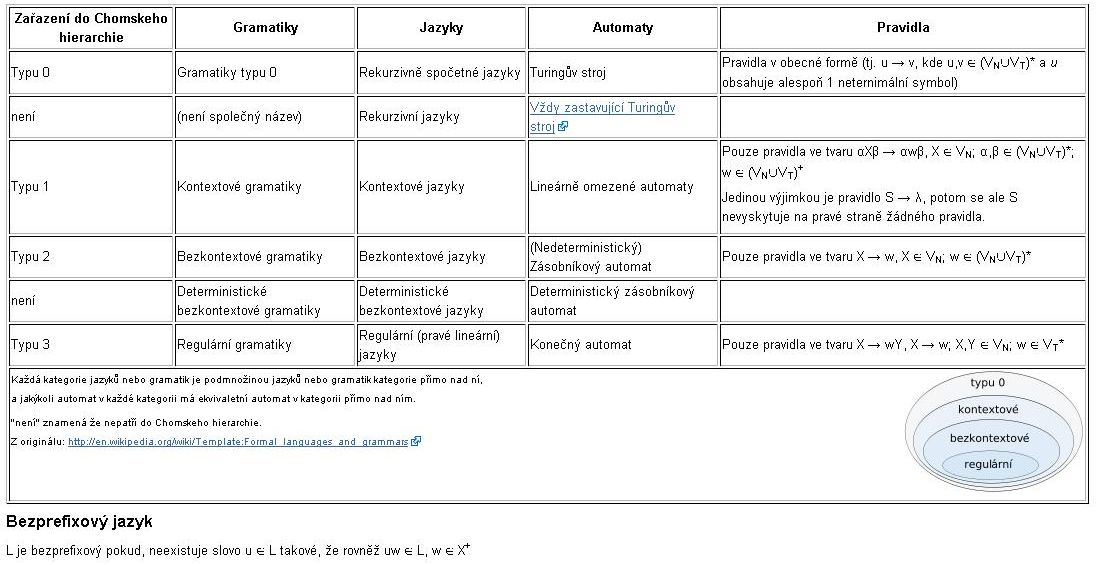
\includegraphics[scale=1.7]{informatika/teoreticka_informatika/obrazky/chomski.png}
  \end{center}
\end{figure}
\end{e}

\begin{e}{Pozn�mka}{0}{0}
S $\c{L}1 \supset \c{L}2$ nast�v� probl�m, proto�e bezkontextov� gramatiky umo��uj� pravidla tvaru $X\to\lambda$. �e�en�m je p�evod na \emph{nevypou�t�j�c� bezkontextov� gramatiky} - takov� bezkontextov� gramatiky, kter� nemaj� pravidla typu $X\to\lambda$.
\end{e}

\begin{e}{V�ta}{0}{o nevypou�t�j�c�ch bezkontextov�ch gramatik�ch}
Ke ka�d� bezkontextov� $G$ existuje nevypou�t�j�c� bezkontextov� $G_0$ tak, �e $$L(G_0)=L(G)\setminus\{\lambda\}$$ Je-li $\lambda\in L(G)$, pak $\exists G_1$, t.�. $L(G_1)=L(G)$ a jedin� pravidlo v $G_1$ s $\lambda$ na prav� stran� je $S\to\lambda$ a $S$ nen� v $G_1$ na prav� stran� ��dn�ho pravidla.
\end{e}

\begin{e}{Pozn�mka}{0}{Line�rn� gramatiky}
Pro ka�dou gramatiku typu G3 lze sestrojit kone�n� automat, kter� p�ij�m� pr�v� jazyk j� generovan�, stejn� tak pro ka�d� kone�n� automat lze sestrojit gramatiku G3. Lev� line�rn� gramatiky tak� generuj� regul�rn� jazyky, d�ky uzav�enosti na reverzi. \emph{Line�rn� gramatiky}, s pravidly typu $X\to uYv,X\to w$, kde $X,Y\in V_N, u,v,w\in V_T^{\ast}$, generuj� \emph{line�rn� jazyky} - siln�j�� ne� regul�rn� jazyky.
\end{e}

\begin{e}{Definice}{0}{Separovan� a nevypou�t�j�c� gramatika}
\emph{Separovan� gramatika} je gramatika (obecn� libovoln� t��dy), obsahuj�c� pouze pravidla tvaru $\alpha\to\beta$, kde bu� $\alpha,\beta\in V_N^+$, nebo $\alpha\in V_N$ a $\beta\in V_T\cup\{\lambda\}$. \emph{Nevypou�t�j�c� (monot�nn�) gramatika} (tak� se neomezuje na konkr�tn� t��du) je takov�, �e pro ka�d� pravidlo $u\to v$ plat� $|u|\leq|v|$.
\end{e}

\begin{e}{Pozn�mka}{0}{Kontextov� gramatiky}
Ke ka�d� kontextov� gramatice lze sestrojit ekvivalentn� separovanou. Ke ka�d� monot�nn� gramatice lze nal�zt ekvivalentn� kontextovou.
\end{e}


\subsubsection*{Determinismus a nedeterminismus}

\begin{e}{Definice}{0}{Nedeterministick� kone�n� automat}
\emph{Nedeterministick� kone�n� automat} je p�tice $(Q,X,\delta,S,F)$, kde $Q$ je mn. stav�, $X$ abeceda, $F$ mn. konc. stav�, $S$ mno�ina po��te�n�ch stav� a $\delta:Q\times X\to \c{P}(Q)$ je p�echodov� funkce. Slovo $w$ je takov�m automatem p�ij�m�no, pokud existuje posloupnost stav� $\{q_i\}_{i=1}^n$ tak, �e $q_1\in S$, $q_{i+1}\in\delta(q_i,x_i)$, $q_{n+1}\in F$.
\end{e}

\begin{e}{Pozn�mka}{0}{0}
Pro ka�d� nedeterministick� kone�n� automat $A$ lze sestrojit deterministick� kon. automat $B$ tak, �e jimi p�ij�man� jazyky jsou ekvivalentn� (m��e to znamenat exponenci�ln� n�r�st po�tu stav�).
\end{e}


\begin{e}{Definice}{0}{Deterministick� z�sobn�kov� automat}
\emph{Deterministick� z�sobn�kov� automat} je $M=(Q,X,Y,\delta,q_0,Z_0,F)$ takov�, �e $\forall p\in Q, \forall a\in (X\cup\{\lambda\}), \forall Z\in Y$ plat� $|\delta(p,a,Z)|\leq 1\footnote{definuje ze v kazdem kroku si nemuzeme vybirat}$ a nav�c pokud pro n�jak� $p, Z$ je $\delta(p,\lambda,Z)\neq\emptyset$, pak $\forall a\in X$ je $\delta(p,a,Z)=\emptyset\footnote{definuje ukon�en� vypoctu}$. 
\end{e}

\begin{e}{Pozn�mka}{0}{0}
Deterministick� z�sobn�kov� automat je \uv{slab��} ne� nedeterministick�, rozpozn�v� \emph{deterministick� bezkontextov� jazyky} koncov�m stavem a \emph{bezprefixov� bezkontextov� jazyky} pr�zdn�m z�sobn�kem (takov� jazyky, kde $u\in L(M)\implies \forall w\in X^{\ast}: uw\notin L(M)$) - kdy� se poprv� z�sobn�k automatu vypr�zdn�, v�po�et ur�it� kon��. 

Bezprefixov� bezkontextov� jazyky jsou v�dy deterministick�, opa�n� to neplat�. Deterministick� bezkontextov� jazyk lze na bezprefixov� p�ev�st z�et�zen�m s dal��m symbolem, kter� nen� v p�vodn� abeced�. 

Regul�rn� jazyky a bezprefixov� bezkontextov� jazyky jsou neporovnateln� mno�iny.
\end{e}

\begin{e}{Definice}{0}{Nedeterministick� Turing�v stroj}
\emph{Nedet. Turing�v stroj} je p�tice $T=(Q,X,\delta,q_0,F)$, kde oproti deterministick�m je $\delta:(Q\setminus F)\times X \to \c{P}(Q\times X\times \{-1,0,1\})$. P�ij�m� slovo $w$, pokud existuje n�jak� v�po�et $q_{0}w\vdash^{\ast} upv$ tak, �e $p\in F$.
\end{e}

\begin{e}{Pozn�mka}{0}{0}
Nedeterministick� Turingovy stroje p�ij�maj� pr�v� rekurzivn� spo�etn� jazyky, tj. nejsou siln�j�� ne� deterministick�. V�po�ty nedet. stroje lze toti� d�ky nekone�nosti p�sky simulovat deterministick�m (nap�. prohled�v�n�m do ���ky).
\end{e}

\begin{e}{Definice}{0}{Line�rn� omezen� automat}
\emph{Line�rn� omezen� automat} je nedeterministick� Turing�v stroj s omezenou p�skou (nap�. symboly $l$ a $r$, kter� nelze p�epsat ani se dostat mimo jejich rozmez�). Slovo je p�ij�m�no, pokud $q_{0}lwr \vdash^{\ast} upv$, kde $p\in F$. Prostor v�po�tu je omezen d�lkou vstupn�ho slova. Line�rn� omezen� automaty p�ij�maj� pr�v� kontextov� jazyky.
\end{e}


\begin{e}{Pozn�mka}{0}{Rozhodnutelnost}
Turing�v stroj m��e nep�ijmout slovo bu� skon�en�m v�po�tu v nekoncov�m stavu, nebo pokud v�po�et nikdy neskon��. Turing�v stroj \emph{rozhoduje jazyk} $L$, kdy� p�ij�m� pr�v� slova tohoto jazyka a pro libovoln� slovo je jeho v�po�et kone�n�. Takov� jazyky se naz�vaj� \emph{rekurzivn�}.

Probl�m zastaven� v�po�tu Turingova stroje je algoritmicky nerozhodnuteln� (kv�li mo�nosti jeho simulace jin�m Turingov�m strojem). Pro bezkontextov� jazyky je algoritmicky rozhodnuteln�, zda dan� slovo pat�� do jazyka. Pro bezkontextovou gramatiku nelze algoritmicky rozhodnout, zda $L(G)=X^{\ast}$. Pro dv� kontextov� gramatiky je nerozhodnuteln�, zda jejich jazyky maj� nepr�zdn� pr�nik.
\end{e}

\begin{reportN}{Hnetynka}
napisal som hierachiu, pravidla gramatik, ake automaty rozpoznavaju jednotlive gramatiky, pre reg gram veticky o KA a reg jazykoch. Pytal sa ma ako jednotlive automaty pracuju, zadal par jednoduchych prikladov a chcel zdovodnenie do akych tried patri -nakreslit/opisat slovami KA, gramatiky, ZA + dokaz pomocou pumping lemma. Pytal sa, do akej triedy by som zaradil rozpoznavanie prg jazykov, napr Java. Povedal som kontextove, ale zdovodnit som to velmi nevedel. Potvrdil ze su to kontextove + ze prave kvoli dobrym znalostam sa pouzivaju bezkontextove v kombinacii s analyzou kontextu (kedze na poradi jednotlivych riadkov zalezi) (znamka 1-2, ze zalezi na druhej inf otazke)
\end{reportN}

\begin{reportN}{Bulej}
napisal som gramatiky, odpovedajuce automaty, vysvetlil inkluzie a to bohato stacilo
\end{reportN}
\begin{reportN}{Bednarek}
M�l jsem definice hierarchie a srovn�n� s p��slu�n�mi automaty, n�stin (opravdu lehce) inkluz� mezi t��dami jazyk�, Greibachov� a Chomsk�ho n.f. plus n�jak� p��klady jazyk�, kter� dokazuj� ostrou inkluzi, ale bez p�esn�j��ch d�kaz� (kouzeln� v�ta: "to se uk�e p�es pumping lemma" ;-) ) Ptal se m� na srovn�n� deterministick�ch a nedeterministick�ch verz� jednotliv�ch druh� automat�, co� jsem v�d�l.
Informatika za jedna.
\end{reportN}
\begin{reportN}{Kucera}
Toto se obeslo bez problemu, stacilo to definovat, a rict ktere automaty prijimaij ktere jazyky, umet je definovat. Vety kolem moc zajem nevzbudily ( Nerudovka, pump. lemma):-) 
\end{reportN}
\begin{reportN}{Fiala}
Napsal sem t��dy automat�, gramatik, determinismus/nedeterminismus a pak je�t� rozhodnutelnost. P�i proch�zen� sem dost�val dopl�uj�c� ot�zky typu : "Jak n�jak l�p omezit odhad o n�rustu po�tu stavu p�i p�evodu NKA do KA" (z�le�� na po�tu po��te�n�ch stav� a na po�tu "stejnejch" p�echod� z jednotliv�ch stav�.), U rozhodnutelnosti n�znak d�kazu halting problem a dal��.
\end{reportN}
\begin{reportN}{Bedn�rek}
Tak jsem napsal automat a gramatiku ke ka�d� t��d� jazyk�, determ./nedeterm. verze a jak je to kde s jejich silou. Drobn� chyby v definic�ch nevadily, kdy� byly po upozorn�n� opraveny. U RJ se zeptal je�t� na reg. v�razy a pak taky pro� �e se rekurzivn� spo�etn� jazyky jmenuj� jak se jmenuj� (kde je ta rekurze), co� jsem nev�d�l a byl pou�en.
\end{reportN}
\begin{reportN}{IOI 10.2.2011} 
a) Popi�te jednotliv� t��dy jazyk� a jejich vztahy definujte t��dy pomoc� odpovidajicich gramatik. Napi�te p�iklady gramatik pro jednotliv� t��dy.
\\b) Popi�te automaty, ktere tyto t��dy jazyk� rozpozn�vaj� i s ohledem na jejich (ne)determinsti�nost.
\end{reportN}
\begin{reportN}{IOI 21. 6. 2011} 4.1 Popi�te Chomsk�ho hierarchii t��d jazyk�, jak se naz�vaj� jazyky v ka�d� t��d�, jak� typ gramatiky je generuje a jak� typ automatu je p�ij�m�.\\
4.2 Uve�te p��klad neregul�rn�ho jazyka a uka�te, �e nen� regul�rn�.\\
\textbf{4.3 Existuje uz�v�rov� vlastnost, na kterou nejsou uzav�en� jazyky typu 0?} TODO
\end{reportN} 
\begin{reportN}{IP 21. 6. 2011} 
Uka�te, �e n�sleduj�c� gramatika G je v�cezna�n� $S \rightarrow if\, then\, S\, else\, S\, | if\, then\, S\, | \lambda$\\
Vytvo�te gramatiku G', kter� nebude v�cezna�n�, a bude platit $L(G) = L(G')$.\\
Existuje obecn� k libovoln� bezkontextov� gramatice G jednozna�n� gramatika G' takov�, �e $L(G) = L(G')$?
\end{reportN} 



\section{Algoritmy a datové struktury}
\begin{pozadavky}
\begin{pitemize}
\item Časová složitost algoritmů, složitost v nejhorším a průměrném případě
\item Třídy složitosti P a NP, převoditelnost, NP-úplnost
\item Binární vyhledávací stromy, vyvažování, haldy
\item Hašování
\item Sekvenční třídění, porovnávací algoritmy, přihrádkové třídění, třídící sítě
\item Grafové algoritmy - prohledávání do hloubky a do šířky, souvislost, topologické třídění, nejkratší cesta, kostra grafu
\item Tranzitivní uzávěr
\item Algoritmy vyhledávání v textu
\item Algebraické algoritmy - DFT, Euklidův algoritmus
\item Základy kryptografie, RSA, DES
\end{pitemize}
\end{pozadavky}
\subsection{�asov� slo�itost algoritm�, slo�itost v nejhor��m a pr�m�rn�m p��pad�}


\begin{e}{Definice}{0}{�asov� slo�itost}
  \textbf{�asovou slo�itost�} algoritmu rozum�me z�vislost jeho �asov�ch n�rok� na
  velikosti konkr�tn�ch vstupn�ch dat. Analogicky se definuje i \textbf{pam�ov�
  slo�itost}. Dobu zpracov�n� �lohy o velikosti $n$ zna��me $T(n)$\\
  �asovou slo�itost �asto zkoum�me z n�kolik hledisek:
  \begin{pitemize}
    \item \textbf{v nejhor��m p��pad�}~-- maxim�ln� po�et operac� pro n�jak� data, 
    \item \textbf{v nejlep��m p��pad�}~-- minim�ln� po�et operac� pro n�jak� data,
    \item \textbf{v pr�m�rn�m (o�ek�van�m) p��pad�}~-- pr�m�r pro v�echna mo�n�
  vstupn� data (n�kdy t� st�edn� hodnota n�hodn� veli�iny $T(n)$).
  \end{pitemize}

  \begin{e}{Pozn�mka}{0}{0}
  Jako jednu \uv{operaci}, nebo-li \emph{krok algoritmu} rozum�me jednu element�rn� 
  operaci n�jak�ho abstraktn�ho stroje (nap�. Turingova stroje), proveditelnou v 
  konstantn�m �ase. Intuitivn�
  je mo�n� ch�pat to jako n�kolik operac� po��ta�e, kter� dohromady netrvaj� v�ce,
  ne� n�jakou pevn� danou dobu.
  \end{e}
\end{e}

\begin{e}{Pozn�mka}{0}{0}
  �asov� slo�itost probl�mu je rovna slo�itosti nejlep��ho algoritmu �e��c�ho
  dan� probl�m.
\end{e}


\subsubsection*{Asymptotick� slo�itost}

\begin{e}{Definice}{0}{0}
  �ekneme, �e funkce $f(n)$ je \textbf{asymptoticky men�� nebo rovna} ne� $g(n)$,
  zna��me $f(n)$ je $O(g(n))$, pr�v� tehdy, kdy�
  $$ \exists c>0\ \exists n_0\ \forall n>n_0: 0 \leq f(n) \leq c \cdot g(n)$$
  Funkce $f(n)$ je \textbf{asymptoticky v�t�� nebo rovna} ne� $g(n)$, zna��me
  $f(n)$ je $\Omega(g(n))$, pr�v� tehdy, kdy�
  $$ \exists c>0\ \exists n_0\ \forall n>n_0: 0 \leq c \cdot g(n) \leq f(n)$$
  Funkce $f(n)$ je \textbf{asymptoticky stejn�} jako $g(n)$, zna��me $f(n)$ je
  $\Theta(g(n))$, pr�v� tehdy, kdy�
  $$ \exists c_1,c_2>0\ \exists n_0\ \forall n>n_0: 0 \leq c_1 \cdot g(n) \leq
  f(n) \leq c_2 \cdot g(n)$$
\end{e}

\begin{e} {Pozn�mka}{0}{0}
  Asymptotick� slo�itost zkoum� chov�n� algoritm� na \uv{velk�ch} datech a dle
  jejich slo�itosti je za�azuje do skupin (polynomi�ln�, exponenci�ln�\dots).
  P�i zkoum�n� se zanedb�vaj� aditivn� a multiplikativn� konstanty. 
\end{e}

\subsubsection*{Amortizovan� slo�itost}

\begin{e}{Definice}{0}{Amortizovan� slo�itost}
  \emph{Amortizovan� �asov� slo�itost} po��t� pr�m�rn� �as na jednu operaci p�i proveden�
  posloupnosti operac�. Pou��v� se typicky pro po��t�n� �asov� slo�itosti operac�
  nad datov�mi strukturami. D�v� realisti�t�j�� horn� odhad slo�itosti
  posloupnosti operac�, ne� po��t�n� s nejhor��m p��padem u ka�d� operace.
\end{e}

\begin{obecne}{Agrega�n� metoda}
  Spo��t�me (nejhor�� mo�n�) �as $T(n)$ pro posloupnost operac�. Amortizovan� cena
  jedn� operace je potom $\frac{T(n)}{n}$.
\end{obecne}

\begin{obecne}{��etn� metoda}
  Od ka�d� operace \uv{vybereme} ur�it� \uv{obnos}, ze kter�ho \uv{zaplat�me} za
  danou operaci a pokud n�co zbude, d�me to na ��et. Pokud je operace dra��� ne�
  kolik je jej� obnos, tak pot�ebn� rozd�l vybereme z ��tu. Z�statek na ��tu
  mus� b�t st�le nez�porn�. Pokud usp�jeme, tak \uv{obnos} = amortizovan� cena
  jedn� operace.
\end{obecne}

\begin{e}{Pozn�mka}{0}{0}
  Jde o to, �e n�kter� operace m��e trvat kr�tce, ale \uv{rozh�e} datovou
  strukturu, tak�e n�sleduj�c� operace pot�ebuj� v�c �asu. Nebo naopak trv�
  dlouho a datovou strukturu \uv{uspo��d�}, tak�e ostatn� operace jsou krat��.
\end{e}

\subsection{T��dy slo�itosti P a NP, p�evoditelnost, NP-�plnost}

TODO: doplnit, tohle asi nestaci na pohodovou zkousku (aspon podle toho co jsem vnimal, jsa svedek zkouseni u Dr. Yaghoba) -- chce to napr. nejaky priklad prevedeni jako delal Kucera, mozna jeste neco

*\subsubsection{P�evoditelnost}

\begin{e}{Definice}{0}{0}
  \begin{pitemize}
  \item \textbf{�loha}~-- Pro dan� zad�n� (vstup, \emph{instanci �lohy}) naj�t v�stup s dan�mi vlastnostmi.
  \item \textbf{Optimaliza�n� �loha}~-- Pro dan� zad�n� naj�t optim�ln� (v�t�inou
  nejmen�� nebo nejv�t��) v�stup s dan�mi vlastnostmi.
  \item \textbf{Rozhodovac� probl�m}~-- Pro dan� zad�n� odpov�d�t ANO/NE. 
  \end{pitemize}
\end{e}

\begin{e}{Definice}{0}{p�evody mezi rozhodovac�mi probl�my}
  Nech� $A$, $B$ jsou dva rozhodovac� probl�my. ��k�me, �e $A$ je
  \textbf{polynomi�ln� redukovateln� (p�evoditeln�)} na $B$, pokud existuje
  zobrazen� $f$ z mno�iny zad�n� probl�mu $A$ do mno�iny zad�n� probl�mu $B$ s
  n�sleduj�c�mi vlastnostmi:
  \begin{pitemize}
    \item Nech� $X$ je zad�n� probl�mu $A$ a $Y$ zad�n� probl�mu $B$, takov�, �e
    $f(X)=Y$. Potom je $X$ kladn� zad�n� probl�mu $A$ pr�v� tehdy, kdy� $Y$ je
    kladn� zad�n� probl�mu $B$.
    \item Nech� $X$ je zad�n� probl�mu $A$. Potom je zad�n� $f(X)$ probl�mu $B$
    (deterministicky sekven�n�) zkonstruovateln� v polynomi�ln�m �ase vzhledem k
    velikosti $X$.
  \end{pitemize}
\end{e}

Jin� definice: M�jme rozhodovac� algoritmus $A$, v�sledek algoritmu ch�pejme jako funkce $A(x)$ na vstupu $x$, pak algoritmus $A$ je redukovateln� na $B$ ($A \rightarrow B$) kdy� $\forall A: B(f(x))=A(x)$ pro polynomi�ln� $f$.

Ob� definice ��kaj�, �e $B$ je \uv{aspo� tak t�k�}, jako $A$ (m��e ale b�t t잚�!). N�zev je trochu zav�d�j�c� -- neredukujeme na \emph{leh��}, ale na \emph{t잚�} algoritmus. Plat� ale, �e pokud $B$ je polynomi�ln� slo�it�, je i $A$.

P�evoditelnost je kvaziuspo��d�n� -- je reflexivn� a tranzitivn�. Nen� ale symetrick� -- na to je pot�eba vytvo�it t��dy slo�itosti, ty potom symetrick� jsou a nad nimi je p�evoditelnost uspo��d�n�.

\begin{e}{Definice}{0}{3-SAT}
 3-SAT (z anglick�ho \uv{satisfiability}) je rozhodovac� probl�m, kter� jako vstup dostane logickou formuli ur�it�ho typu a rozhodne, zda je, nebo nen� plniteln�, tj. jestli existuje n�jak� jej� ohodnocen�, kter� je pravdiv�. Logick� formule mus� b�t n�sleduj�c�ho typu:

$$(a_1\vee b_1 \vee c_1) \wedge (a_2 \vee b_2 \vee c_2) .... \wedge (a_n \vee b_n \vee c_n),$$

kde $a_n, b_n, c_n$ jsou bu� $x_i$ nebo $\not x_i$ pro n�jak� $i\subset \mathbb{N}$.
\end{e}

\begin{e}{Definice}{0}{3-COL}
3-COL, nebo tak� trojbarevnost grafu, je n�sleduj�c� probl�m: dostanu graf a mus�m ur�it, jestli jej lze obarvit t�emi barvami.
\end{e}

\begin{e}{Definice}{0}{Probl�m nez�visl� mno�iny v grafu}
Probl�m nez�visl� mno�iny v grafu:
Existuje v dan�m grafu velikosti $N$ nez�visl� mno�ina velikosti $K$?
\end{e}

\begin{e}{V�ta}{0}{0}
3-SAT $\rightarrow$ 3-COL

\begin{e}{D�kaz}{0}{0}
Pro 3-SAT si ud�l�me graf�k, kter� bude obarviteln� $\Leftrightarrow$ 3-SAT m� �e�en�.

Pravdu si budu v grafu reprezentovat jako b�lou, nepravdu jako �ernou, t�et� barva je pomocn�.

Nejd��ve si ud�l�m \uv{konstrukt}, co mi pro ka�dou kombinaci t�� barev \uv{vr�t�} logick� or.

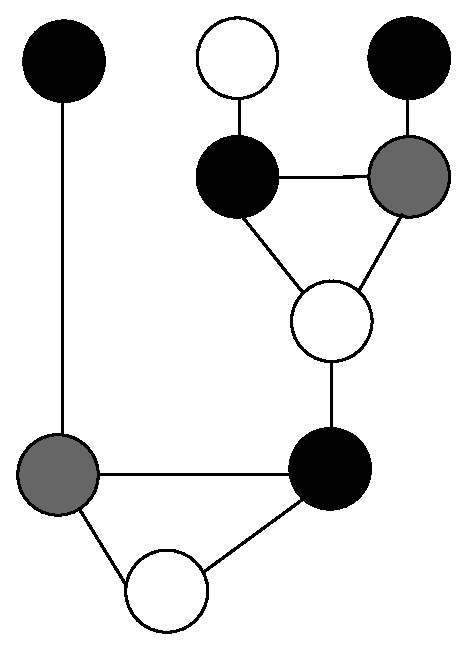
\includegraphics[width=0.1\textwidth]{informatika/teoreticka_informatika/obrazky/3COL1}

Kdy� do v��e uveden�ho konstruktu jakoby \uv{vlo��m} do horn� ��dky barvy, odpov�daj�c� t�� pravdivostn�m hodnot�m, nem��u spodn� vrchol obarvit jinak, ne� jako logick� or t�� barev. Tyto konstrukty mi budou slou�it pro reprezentaci $(a \vee b \vee c)$.

Ud�l�m si te� jeden st�edn� bod ($C$ jako centrum), k~n�mu p�id�m nejd��v dva body $T$ a $F$ a potom pro ka�dou prom�nnou p�id�m dva body, reprezentuj�c� $x$ a $\not x$ a spoj�m je dohromady a s~$C$. Ne� za�nu p�id�vat \uv{konstrukty} na vyhodnocov�n� trojic, pod�v�m se na vlastnosti. Mus� platit:

\begin{itemize}
\item $C$, $T$ a $F$ mus� m�t ka�d� jinou barvu
\item pro v�echny body mus� b�t bu� $x$ nebo $\not x$ $T$ barva a ta druh� $F$ barva
\end{itemize}

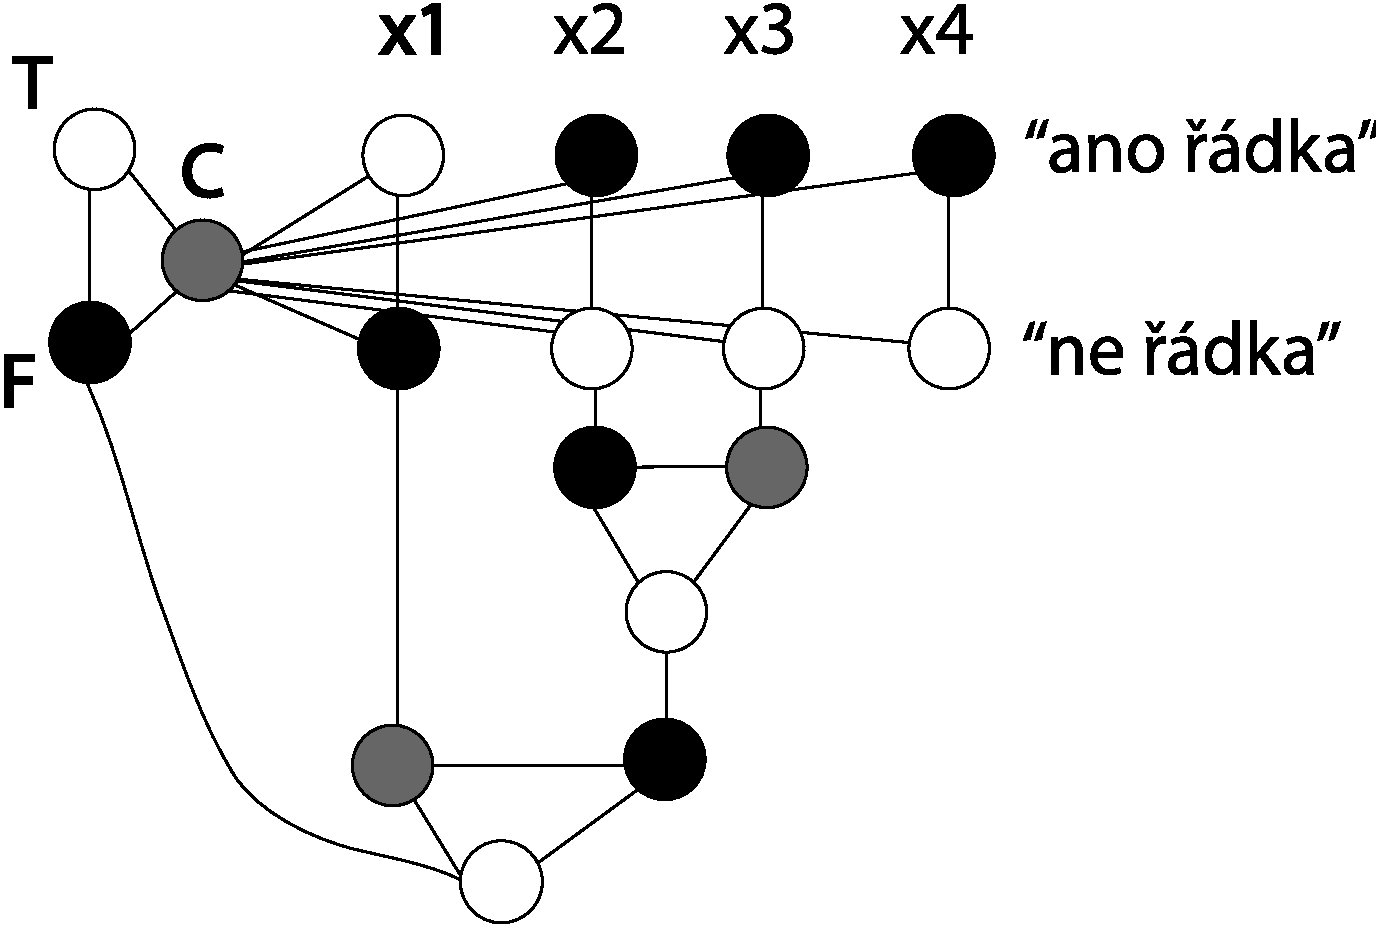
\includegraphics[width=0.8\textwidth]{informatika/teoreticka_informatika/obrazky/3COL2}

B�NO m��u ��ct, �e $C$ je �ediv�, $T$ b�l� a $F$ �ern�, �ern� mi vyjad�uje nepravdu, b�l� pravdu. Potom za n� \uv{nav�s�m} ty konstrukty -- bu� na $x$, nebo na $\not x$, podle toho, kter� z nich ve trojici zrovna je --  a jejich spodn� vrchol p�ipoj�m $F$�vrchol (to \uv{vynucuje}, aby vrchol byl $T$). Na obr�zku je formule $(\not x_1 \vee \not x_2 \vee \not x_3)$.

Tento graf je obarviteln� pr�v� tehdy, kdy� je formule splniteln�, a je sestaviteln� v~polynomi�ln�m �ase.

\end{e}
\end{e}

\begin{e}{Definice}{0}{t��da P}
 \textbf{T��du slo�itosti P} (n�kdy t� PTIME) tvo�� probl�my �e�iteln�
 sekven�n�mi deterministick�mi algoritmy v polynomi�ln�m �ase, tj. jejich �asov�
 slo�itost je $O(n^k)$. O algoritmech ve t��d� P tak� ��k�me, �e jsou
 \textbf{efektivn� �e�iteln�.}
\end{e}

\begin{e}{Definice}{0}{t��da NP}
 \textbf{T��da NP} (NPTIME) je t��da probl�m� �e�iteln�ch v polynomi�ln�m �ase
 sekven�n�mi nedeterministick�mi algoritmy. 
\end{e}

\begin{e}{Pozn�mka}{0}{0}
  V� se, �e $P \subseteq NP$. Nev� se v�ak, zda $P \neq NP$. P�edpokl�d� se to,
  ale je�t� to nikdo nedok�zal.
\end{e}

\begin{obecne}{P��klady probl�m� ze t��dy NP}
  \begin{pitemize}
    \item \textbf{KLIKA}(�pln� podgraf)~-- Je d�n neorientovan� graf $G$ a ��slo
    $k$. Existuje v $G$ �pln� podgraf velikosti aspo� $k$?
    \item \textbf{HK}(Hamiltonovsk� kru�nice)~-- Je d�n neorientovan� graf $G$.
    Existuje v $G$ Hamiltonovsk� kru�nice?
    \item \textbf{SP}(Sou�et podmno�iny)~-- Jsou d�na p�irozen� ��sla $a_1,
    \dots, a_n,b$. Existuje podmno�ina ��sel $a_1,\dots,a_n$, jej� sou�et je
    p�esn� $b$?
  \end{pitemize}
\end{obecne}

\begin{e}{Definice}{0}{NP-t�k� probl�m}
  Probl�m $B$ je \textbf{NP-t�k�}, pokud pro libovoln� probl�m $A$ ze t��dy NP
  plat�, �e $A$ je polynomi�ln� redukovateln� na $B$.
\end{e}

\begin{e}{Definice}{0}{NP-�pln� probl�m}
  Probl�m je \textbf{NP-�pln�}, pokud pat�� do t��dy NP a je NP-t�k�.
\end{e}

\begin{obecne}{D�sledky}
  \begin{pitemize}
    \item Pokud je $A$ NP-t�k� a nav�c je $A$ polynomi�ln� redukovateln� na $B$, tak je
      $B$ taky NP-t�k�.
    \item Pokud existuje polynomi�ln� algoritmus pro n�jak� NP-t�k� probl�m, pak
      existuj� polynomi�ln� algoritmy pro v�echny probl�my ve t��d� NP.
  \end{pitemize}
\end{obecne}

\begin{e}{V�ta}{0}{Cook-Levin 1971}
 Existuje NP-�pln� probl�m. (Dok�z�no pro SAT)
\end{e}

\def\b#1{\mathbf{#1}}


\subsection{Bin�rn� vyhled�vac� stromy, vyva�ov�n�, haldy}

\subsubsection*{Bin�rn� strom}

\begin{e}{Definice}{0}{0}
\emph{Dynamick� mno�ina} je mno�ina prvk� (datov� struktura), m�n�c� se v �ase. Ka�d� jej� prvek je p��stupn� p�es ukazatel a obsahuje:
\begin{pitemize}
    \item \emph{kl��} (jednu polo�ku, typicky hodnotu z lin. uspo��dan� mno�iny), 
    \item \emph{ukazatel(e)} na dal�� prvky, 
    \item p��padn� \emph{dal�� data}.
\end{pitemize}
Na takov� mno�in� jsou definov�ny tyto operace:
\begin{pitemize}
    \item \emph{find} - nalezen� prvku podle kl��e
    \item \emph{insert} - p�id�n� dal��ho prvku
    \item \emph{delete} - odstran�n� prvku
    \item \emph{min}, \emph{max} - nalezen� nejv�t��ho / nejmen��ho prvku
    \item \emph{succ}, \emph{pred} - nalezen� n�sleduj�c�ho / p�edch�zej�c�ho prvku k n�jak�mu p�edem dan�mu
\end{pitemize}
\end{e}


\begin{e}{Definice}{0}{0}
\emph{Bin�rn� strom} je dynamick� mno�ina, kde ka�d� prvek (uzel, node) m� krom� kl��e a p��p. dal��ch dat t�i ukazatele na \emph{lev�ho} a \emph{prav�ho} syna a rodi�e. Speci�ln� uzel je \emph{ko�en}, kter� m� NULLov� ukazatel na rodi�e. Ten je v bin�rn�m strom� jeden. Uzly, kter� maj� NULLov� ukazatele na prav�ho i lev�ho syna, se naz�vaj� \emph{listy}.

\emph{Podstrom} je ��st stromu (vybran� prvky), kter� je sama stromem - nap�. pokud se jako ko�en ur�� jeden z prvk�. \emph{Lev�(prav�)} podstrom n�jak�ho prvku je strom, ve kter�m je ko�enem lev�(prav�) syn tohoto prvku. \emph{V��ka stromu} je d�lka nejdel�� cesty od ko�enu k listu.
\end{e}

Bin�rn� strom je \emph{vyv�en�}, pokud max. 1 uzel m� jednoho syna (tj. v�echny vnit�n� uzly krom� a� na jeden maj� oba syny, listy z definice nemaj� ��dn�ho). V��ka vyv�en�ho stromu roste logaritmicky vzhledem k po�tu uzl�. V��ka nevyv�en�ho stromu m��e r�st a� line�rn� vzhledem k po�tu prvk� (i \uv{spojov� seznam} je platn� bin. strom).


\subsubsection*{Bin�rn� vyhled�vac� strom}

\begin{e}{Definice}{0}{0}
\emph{Bin�rn� vyhled�vac� strom} je takov� bin�rn� strom, ve kter�m je jeho struktura ur�en� podle kl��u jeho uzl�: pro ka�d� uzel s kl��em hodnoty $k$ plat�, �e jeho lev� podstrom obsahuje jen uzly s men�� hodnotou kl��e ne� $k$ a jeho prav� podstrom jen uzly s hodnotou kl��e v�t�� nebo rovnou $k$.
\end{e}

\begin{e}{Algoritmus}{0}{Vyhled�v�n� v bin. strom�}
\begin{verbatim}
Find( x - ko�en, k - hledan� hodnota kl��e ){
  while( x != NULL && k != x->kl�� ){
    if ( k < x->kl�� )
      x = x->lev�_syn;
    else
      x = x->prav�_syn;
  }
  return x;
}
\end{verbatim}

Slo�itost je $O(h)$ v nejhor��m p��pad�, kde $h$ je v��ka stromu (tj. pro nevyv�en� stromy a� $O(n)$ kde $n$ je po�et prvk�). Asymptotick� �asov� slo�itost ostatn�ch operac� je stejn�.

Vlo�en� a vymaz�n� prvku se prov�d� prost�m nalezen�m m�sta, kam by se prvek m�l vlo�it (nebo kde u� je), a p�epojen�m pointer�.
\end{e}

\subsubsection*{Vyva�ovan� vyhled�vac� stromy}

Kv�li zaji�t�n� v�t�� rychlosti (men�� asymptotick� �asov� slo�itosti) operac� byly vytvo�eny speci�ln� druhy bin�rn�ch vyhled�vac�ch strom�, kter� jsou pr�b�n� vyva�ov�ny, aby m�ly max. v��ku men�� ne� $c\cdot\log n$, kde $n$ je po�et uzl� a $c$ n�jak� konstanta.

\begin{e}{Definice}{0}{Pomocn� operace na stromech}
Pro vyva�ov�n� strom� p�i vkl�d�n� a odeb�r�n� uzl� se definuj� pomocn� operace: \emph{prav�} a \emph{lev� rotace}. Zachov�vaj� vlastnosti bin. vyhled�vac�ch strom� a jsou provediteln� v konstatn�m �ase - jde jen o p�epojen� uzl� n�sl. zp�sobem (pro pravou rotaci na uzlu $Q$ a levou na $P$):

\begin{center}
\includegraphics[width=12cm]{informatika/algoritmy_a_ds/obrazky/tree_rotation.png}

(Zdroj obr�zku: Wikipedia)
\end{center}
\end{e}


\begin{e}{Definice}{0}{�erveno-�ern� stromy}
�erveno-�ern� stromy jsou bin�rn� vyhled�vac� stromy s garantovanou max. v��kou $O(\log n)$, kde $n$ je po�et uzl�, tj. operace na nich mohou m�t asymptotickou �asovou slo�itost $O(\log n)$. Pro jejich popis je nutn� definovat \emph{intern� uzly} - v�echny uzly stromu a \emph{extern� uzly} - na (intern�ch) listech (a uzlech s jedn�m potomkem) um�le p�idan� NULLov� ukazatele (de facto \uv{listy} �erveno-�ern�ho stromu). Extern� uzly slou�� jenom jako abstrakce pro popis strom�, p�i implementaci se s nimi neoperuje. �erveno-�ern� strom m� tyto �ty�i povinn� vlastnosti:
\begin{penumerate}
    \item Ka�d� uzel (extern� i intern�) m� definovanou barvu, a to �ernou nebo �ervenou.
    \item Ka�d� extern� uzel je �ern�.
    \item Ka�d� �erven� vrchol mus� m�t oba syny �ern�.
    \item Ka�d� cesta od libovoln�ho vrcholu k list�m v jeho podstrom� mus� obsahovat stejn� po�et �ern�ch uzl�.
\end{penumerate}

Pro �erveno-�ern� stromy se definuje \emph{v��ka uzlu} $x$ ($\b{h}(x)$) jako po�et uzl� na nedel�� mo�n� cest� k listu v jeho podstrom�. \emph{�ern� v��ka uzlu} ($\b{bh}(x)$) je po�et �ern�ch uzl� na takov� cest�.
\end{e}

\begin{e}{V�ta}{0}{Vlastnosti �erveno-�ern�ch strom�}
Podstrom libovoln�ho uzlu $x$ obsahuje alespo� $2^{\b{bh}(x)}-1$ intern�ch uzl�. D�ky tomu m� �erveno-�ern� strom v��ku v�dy nejv��e $2\log(n+1)$ (kde $n$ je po�et uzl�). (D�kaz prvn�ho tvrzen� indukc� podle $\b{h}(x)$, druh�ho z prvn�ho a t�et� vlastnosti �erveno-�ern�ch strom�)
    \end{e}

\begin{e}{D�sledek}{0}{0}
Operace hled�n� (minima, maxima, n�sledn�ka, \dots), kter� jsou stejn� jako u obecn�ch bin�rn�ch vyhled�vac�ch strom�, maj� garantovanou �asovou slo�itost $O(\log n)$.
\end{e}

\begin{e}{Algoritmus}{0}{Vkl�d�n� a odeb�r�n� uzl� v �erveno �ern�ch stromech}
Ob� operace maj� podle garantovan� max. v��ky garantovanou �as. slo�itost $O(\log n)$ pro $n$ po�et uzl�. Proto�e bez poru�en� vlastnost� �erveno-�ern�ch strom� lze ko�en v�dy p�ebarvit na�erno, m��eme pro n� p�edpokl�dat, �e \emph{ko�en stromu} je \emph{v�dy �ern�}.

\emph{Vkl�d�n�} vypad� n�sledovn�:
\begin{pitemize}
    \item Nalezen� m�sta pro vlo�en� a p�id�n� nov�ho prvku jako v obecn�ch bin. vyhl. stromech, nov� prvek se p�ebarv� na�erveno.
    \item Pokud je jeho otec �ern�, m��eme skon�it -- vlastnosti strom� jsou spln�n�. Pokud je �erven�, mus�me strom upravovat (tady p�edpokl�d�m, �e otec p�id�van�ho uzlu je lev�m synem, opa�n� p�ipad je symetrick�):
    \item Je-li i str�c �erven�, p�ebarvit otce a str�ce na�erno a p�en�st chybu o patro v�� (je-li d�d �ern�, kon��m, jinak m��u pokra�ovat a� do ko�ene, kter� u� lze p�ebarvovat beztrestn�).
    \item Je-li str�c �ern� a p�idan� uzel je lev�m synem, ud�lat pravou rotaci na d�dovi a p�ebarvit uzly tak, aby odpov�daly vlastnostem strom�.
    \item Je-li str�c �ern� a p�idan� uzel je prav�m synem, ud�lat levou rotaci na otci a p�ev�st tak na p�edchoz� p��pad.
\end{pitemize}

\emph{Odeb�r�n�} se prov�d� takto:
\begin{pitemize}
    \item Odstran�m uzel stejn� jako v p�edchoz�m p��pad�. Opravdu odstran�n� uzel (z p�epojov�n�) m� max. jednoho syna. Pokud odstra�ovan� uzel byl �erven�, neporu��m vlastnosti strom�, stejn� tak pokud jeho syn byl �erven� -- to �e��m jeho p�ebarven�m na�erno.
    \item V opa�n�m p��pad� (tj. syn odeb�ran�ho -- $x$ -- je �ern�) mus�m ud�lat n�sl. �pravy (p�ep. �e $x$ je lev�m synem sv�ho nov�ho otce, v op. p��pad� postupuji symetricky):
    \item $x$ prohl�s�m za \uv{dvojit� �ern�} a t�to vlastnosti se pokou��m zbavit.
    \item Pokud je bratr $x$ (bu� $w$) �erven�, pak m� 2 �ern� syny -- provedu levou rotaci na rodi�i $x$, prohod�m barvy rodi�e $x$ a uzlu $w$ a p�evedu tak situaci na jeden z n�sl. p��pad�:
    \item Je-li $w$ �ern� a m�-li 2 �ern� syny, prohl�s�m $x$ za �ern� a p�ebarv�m $w$ na�erveno, rodi�e p�ebarv�m bu� na �erno (a kon��m) nebo na \uv{dvojit� �ernou} a propaguji chybu (mohu doj�t a� do ko�ene, kter� lze p�ebarovat beztrestn�).
    \item Je-li $w$ �ern�, jeho lev� syn �erven� a prav� �ern�, vym�n�m barvy $w$ s jeho lev�m synem a na $w$ pou�iji pravou rotaci, ��m� dostanu posledn� p��pad:
    \item Je-li $w$ �ern� a jeho prav� syn �erven�, p�ebarv�m prav�ho syna na�erno, odstran�m dvojit� �ernou z $x$, provedu levou rotaci na $w$ a pokud m�l p�vodn� $w$ (a $x$) �erven�ho otce, p�ebarv�m $w$ na�erveno a tohoto (te� u� lev�ho syna $w$) p�ebarv�m na�erno.
\end{pitemize}
\end{e}


\begin{e}{Definice}{0}{AVL stromy (Adelson-Velsky \& Landis)}
\emph{AVL stromy} jsou, podobn� jako �erveno-�ern� stromy, bin. vyhled�vac� stromy, kter� zaru�uj� max. logaritmick� n�r�st v��ky vzhledem k po�tu prvk�. Pro ka�d� uzel $x$ se v AVL stromu definuje \emph{faktor vyv�en�} jako rozd�l v��ky jeho lev�ho a prav�ho podstromu: $\b{bf}(x) = h(\texttt{x->lev�}) - h(\texttt{x->prav�})$. Pro v�echny uzly v AVL stromu plat�, �e $|\b{bf}(x)|\leq 1$.
\end{e}

\begin{e}{V�ta}{0}{Zaru�en� v��ky AVL strom�}
V��ka AVL stromu s $n$ vrcholy je $O(\log n)$. (D�kaz: bu� $T_n$ AVL strom v��ky $n$ s minim�ln�m po�tem uzl�. Ten m� podstromy $T_{n-1}$ a $T_{n-2}$ atd., tj. velikost minim�ln�ho AVL stromu roste jako Fibonacciho posloupnost, tedy $|T_n|\geq (\frac{1+\sqrt{5}}{2})^{n-1}$. D�kaz tohoto indukc�.)
\end{e}

\begin{e}{Algoritmus}{0}{Operace na AVL stromech}
Vyhled�vac� operace se prov�d� stejn� jako na obecn�ch bin. vyhled�vac�ch stromech, vkl�d�n� a odeb�r�n� prvk� taky, ale pokud tyto operace poru�� z�kl. vlastnost AVL strom� ($|\b{bf}(x)=2|$), je nutn� prov�st vyva�ov�n� -- pomoc� rotac� (kter� mohou b�t propagov�ny a� ke ko�eni). P�i vkl�d�n� a odeb�r�n� je nav�c nutn� pr�b�n� (nejh��e a� ke ko�eni) upravovat indikaci faktoru vyv�en� jednotliv�ch uzl�.
\end{e}

\subsubsection*{Halda}

\begin{e}{Definice}{0}{0}
\emph{Halda(heap)} je dynamick� mno�ina se stromovou strukturou (bin�rn� halda je bin�rn� strom), pro kterou plat� tzv. \uv{vlastnost haldy}: $$\text{ Je-li }x\text{ potomek }y\text{, pak }x\texttt{->kl��}\geq y\texttt{->kl��}$$ Haldy s touto nerovnost� jsou tzv. \emph{min-heap}y, pokud je nerovnost opa�n�, jde o \emph{max-heap}.
\end{e}

\begin{obecne}{(Bin�rn�) haldy}
Bin�rn� haldy jsou nej�ast�j��m typem haldy. Zaji��uj� nalezen� minim�ln�ho prvku v konstantn�m �ase a odebr�n� a p�id�n� minima v �ase $O(\log n)$. V ka�d� hladin� od prvn� a� do p�edposledn� je max. mo�n� po�et uzl�, v posledn� jsou uzly co nejv�ce \uv{vlevo} -- tedy max. v��ka haldy s $n$ prvky je $(\log n) + 1$. Proto je pro bin�rn� haldy jednodu�e provediteln� jejich datov� reprezentace polem (bez pointer�), kde p�i indexov�n� od 0 m� uzel na indexu $k$:
\begin{pitemize}
    \item Lev�ho a prav�ho syna na indexu $2k+1$, resp. $2k+2$ (pokud to nen� v�c ne� celk. po�et prvk�, potom syny nem�).
    \item Rodi�e na indexu $\lceil\frac{k}{2}\rceil-1$. 
\end{pitemize}

\emph{P�id�n� uzlu} do haldy znamen� p�id�n� prvku na konec haldy a dokud m� jeho rodi� v�t�� kl��, jeho prohazov�n� s rodi�em (tedy posouv�n� o vrstvu v��). P�i \emph{odeb�r�n� uzlu} z haldy tento nahrad�m posledn�m prvkem v hald� a potom dokud neplat� vlastnost haldy (nejm�n� jeden z potomk� m� men�� kl��), prohazuji ho s potomkem s men��m kl��em (a posouv�m o vrstvu n�).

Vytvo�en� haldy je mo�n� v �ase $O(n)$, kde $n$ je po�et prvk� v hald� -- p�id�n� 1 prvku do haldy trv� $O(h)$, kde $h$ je aktu�ln� v��ka (a $h$ roste od $0$ a� k $\lceil\log n\rceil$, po�et prvk� ve v��ce $k$ je $\frac{n}{2^{k+1}}$, bereme-li v��ku list� rovnou nule) - v sou�tu za v�echny prvky jde o $O(n\cdot\sum_{h=0}^{\lceil\log n\rceil}\frac{h}{2^h})$.

Bin�rn� halda se pou��v� nap�. k \emph{t��d�n� haldou} (heapsortu), kdy se z dat, kter� je pot�eba ut��dit, nejd��ve postav� halda, a potom se opakuje operace odebr�n� ko�ene (tj. minim�ln�ho prvku).
\end{obecne}

\begin{obecne}{Fibonacciho haldy}
Fibonacciho haldy maj� n�zkou �asovou slo�itost b�n�ch operac� -- amortizovan� $O(1)$ pro vlo�en�, hled�n� minima apod.; odebr�n� prvku a odebr�n� minima m� slo�itost $O(\log n)$ pro $n$ prvk� v hald�. Tvo�� ji skupina strom�, vyhovuj�c�ch \uv{vlastnosti haldy}. Ka�d� uzel haldy s $n$ prvky m� max. $\log n$ potomk� a ve sv�m podstrom� minim�ln� $F_{k+2}$ uzl�, kde $F_k$ je $k$-t� Fibonacciho ��slo. To je zaji�t�no pravidlem, �e p�i odeb�r�n� prvk� lze z neko�enov�ho uzlu odd�lit max. 1 syna, jinak je nutn� odd�lit i tento uzel a ten se pak stane ko�enem dal��ho stromu. Po�et strom� se sni�uje p�i odeb�r�n� minima, kdy jsou spojov�ny dohromady.

Fibonacciho haldy se pou��vaj� pro efektivn� implementaci slo�it�j��ch operac�, jako nap�. Jarn�kova nebo Dijkstrova algoritmu.
\end{obecne}

\newcommand{\nadpis}[1]{\pagebreak[2]\ramcek{\subsubsection*{#1}}}

\subsection{Hašování}

\begin{definiceN}{slovníkový problém} Dáno univerzum $U$, máme reprezentovat
$S \subseteq U$ a navrhnout algoritmy pro operace
\begin{pitemize}
\item MEMBER(x) - zjistí zda $x \in S$ a pokud ano nalezne kde,
\item INSERT(x) - pokud $x \notin S$, vloží $x$ do struktury reprezentující $S$,
\item DELETE(x) - když $x \in S$, smaže $x$ ze struktury reprezentující $S$.
\end{pitemize}
\end{definiceN}

Například pomocí pole můžeme tyto operace implementovat rychle, ale nevýhodou
je prostorová náročnost. Pro velké množiny je to někdy dokonce nemožné.
\emph{Hašování} se snaží zachovat rychlost operací a odstranit prostorovou
náročnost.

Podívejme se nyní na \emph{základní ideu} hašování. Mějme univerzum $U$ a
množinu $S \subseteq U$ takovou, že $|S| << |U|$. Dále mějme funkci
$h:U\rightarrow\{0,1,\dots,m-1\}$. Množinu $S$ potom reprezentujeme tabulkou
(polem) o velikosti $m$ tak, že prvek $x \in S$ je uložen na řádku $h(x)$.

\begin{definiceN}{Hašovací funkce, kolize} Funkci
$h:U\rightarrow\{0,1,\dots,m-1\}$ potom nazýváme \textbf{hašovací funkcí}.
Situaci $h(s)=h(t)$, pro $s \neq t; s,t \in S$  nazveme \textbf{kolize}.
\end{definiceN}

Jelikož mohutnost univerza $U$ je větší než velikost hašovací tabulky, nelze se
kolizím úplně vyhnout. Existuje spousta různých metod, jak kolize řešit.
Podívejme se tedy na některé podrobněji.

\begin{definice}
Ještě si zavedeme některé značení. Velikost $S$ (hašované množiny) označme
\textbf{n}, velikost tabulky (pole) označme \textbf{m}, a faktor naplnění
\textbf{$\alpha=\frac{n}{m}$}.
\end{definice}

\subsubsection*{Hašování se separovanými řetězci}

Použijeme pole velikosti $m$, jehož $i$-tá položka bude spojový seznam $S_i$
takový, že $s\in S_i \Leftrightarrow h(s)=i$, pro $s\in S$. Čili každý řádek
pole obsahuje spojový seznam všech (kolidujících) prvků, které jsou hašovány na
tento řádek. Seznamy nemusí být uspořádané, vznikají tak, jak jsou vkládány
jednotlivé prvky do struktury.

\begin{algoritmusN}{Hašování se separovanými řetězci}
\begin{pitemize}
\item \textbf{MEMBER} -- Spočteme hodnotu hašovací funkce $h(x)$, prohledáme
řetězec začínající na pozici $h(x)$ a zjistíme zda se prvek nachází, či
nenachází ve struktuře. Pokud se prvek v databázi nachází, tak musí nutně ležet
v tomto řetězci.
\item \textbf{INSERT} -- Zjistíme zda $x$ je v řetězci $h(x)$, pokud ne, přidáme
ho nakonec, v opačném případě neděláme nic.
\item \textbf{DELETE} -- Vyhledá $x$ v řetězci $h(x)$ a smaže ho. Pokud se tam
$x$ nenachází, neudělá nic.
\end{pitemize}
\end{algoritmusN}

\paragraph{Očekávaný počet testů} v neúspěšném případě je přibližně
$e^{-\alpha} + \alpha$ a při úspěšném vyhledávání přibližně
$1+\frac{\alpha}{2}$.

\subsubsection*{Hašování s uspořádanými řetězci}

Jak již je zřejmé z názvu je tato metoda téměř stejná jako předchozí. Jediný
rozdíl je, že jednotlivé seznamy jsou uspořádány vzestupně dle velikosti
prvků.

\begin{algoritmusN}{Hašování s uspořádanými řetězci}
Rozdíly jsou pouze pro operaci \textbf{MEMBER}, kde skončíme prohledávání, když
dojdeme na konec, nebo když nalezneme prvek, který je větší než hledaný a
operaci \textbf{INSERT}, které vkládá prvek na místo kde jsme ukončili
vyhledávání (před prvek, který ho ukončil).
\end{algoritmusN}

\paragraph{Očekávaný počet testů} v neúspěšném případě je přibližně roven
$e^{-\alpha}+1+\frac{\alpha}{2}-\frac{1}{\alpha}(1-e^{-\alpha})$ a v úspěšném
případě je přibližně $1+\frac{\alpha}{2}$.

Nevýhodou předchozích dvou metod je nerovnoměrné využití paměti. Zatímco
některé seznamy mohou být dlouhé, v některých není prvek žádný. Řešením je najít
způsob, jak kolidující prvky ukládat na jiné (prázdné) řádky tabulky. Potom je
ale nutné každý prvek tabulky rozšířit a položky pro práci s tabulkou. 

Čím použijeme sofistikovanější metodu ukládání dat do tabulky, tím více budeme
potřebovat položek pro práci s tabulkou a tedy vzroste paměťová náročnost. Naším
cílem je tedy najít rozumný kompromis mezi sofistikovaností (rychlostí)
strategie a její paměťovou náročností. Podívejme se na další algoritmy,
které se o to pokoušejí.

\subsubsection*{Hašování s přemísťováním}

Seznamy jsou tentokrát ukládány do tabulky a implementovány jako dvousměrné.
Potřebujeme tedy dvě položky pro práci s tabulkou: \emph{next} -- číslo řádku
obsahující další prvek seznamu a \emph{previous} -- číslo řádku obsahující
předchozí prvek seznamu. Když dojde ke kolizi, tj. chceme vložit prvek a jeho
místo je obsazené prvkem z jiného řetězce, pak tento prvek z jiného řetězce
přemístíme na jiný prázdný řádek v tabulce (proto hašování s přemísťováním).

\begin{algoritmusN}{Hašování s přemísťováním}
Algoritmus \textbf{MEMBER} funguje stejně jako u hašování se separovanými
řetězci, jen místo ukazatele na další prvek použije hodnotu \emph{next} z
tabulky. Při operaci \textbf{INSERT} vložíme prvek kam patří pokud je tam místo,
pokud již je místo obsazeno prvkem který tam patří, čili zde začíná seznam
kolidujících prvků (\emph{previous} = prázdné), pak postupujeme po položkách
\emph{next} až na konec seznamu, vložíme prvek na některý volný řádek
tabulky a vyplníme správně hodnoty \emph{next} a \emph{previous}. Pokud je místo
obsazeno prvkem z jiného seznamu (\emph{previous} $\neq$ prázdné), tak tento
prvek přemístíme na některý volný řádek, správně přepíšeme položky \emph{next} a
\emph{previous} v měněném seznamu a vkládaný prvek uložíme na jeho místo.
Operace \textbf{DELETE} je vcelku přímočará, jenom je třeba, pokud mažeme první
prvek seznamu na jeho místo přesunout ten druhý v pořadí (pokud existuje).
\end{algoritmusN}

\paragraph{Očekávaný počet testů} je v neúspěšném případě roven přibližně
$(1-\frac{1}{m})^n+\frac{n}{m}\approx e^{-\alpha}+\alpha$ a v úspěšném je stejný
jako pro hašování se separovanými řetězci a tedy $\frac{n-1}{2m}+1 \approx 1 +
\frac{1}{\alpha}$.

\subsubsection*{Hašování se dvěma ukazateli}

Hašování s přemísťováním má tu nevýhodu, že díky přemisťování prvků jsou operace
INSERT a DELETE časově náročné. Tato metoda tedy implementuje řetězce jako
jednosměrné seznamy, ale takové které nemusejí začínat na svém místě, tj.
řetězec $S_j$ obsahující prvky $s \in S$ takové, že $h(s)=j$, nemusí začínat na
$j$-tém řádku. Místo ukazatele na předchozí prvek tak do položek pro práci s
tabulkou přidáme ukazatel na místo, kde začíná řetězec příslušný danému řádku.
Položky pro práci s tabulkou tedy budou: \emph{next} -- číslo řádku tabulky kde
je další prvek seznamu, \emph{begin} -- číslo řádku tabulky obsahující první
prvek seznamu příslušného tomuto místu.

\begin{algoritmusN}{Hašování se dvěma ukazateli}
Položka \emph{begin} v $j$-tém řádku je vyplněna právě tehdy, když
reprezentovaná množina $S$ obsahuje prvek $s \in S$ takový, že $h(s)=j$.
Algoritmy jsou potom podobné těm u hašování s přemísťováním, ale přemísťování
prvků je nahrazeno odpovídajícími změnami v položce \emph{begin} daných řádků.
\end{algoritmusN}

Díky práci s položkami jsou operace INSERT a DELETE rychlejší než při hašování s
přemísťováním, ale začátek řetězce v jiném řádku tabulky přidá navíc jeden test,
což změní složitost operace MEMBER.

\paragraph{Očekávaný počet testů} v neúspěšném případě je přibližně
$1+\frac{\alpha^2}{2}+\alpha+e^{-\alpha}(2+\alpha)-2$ a při úspěšném vyhledávání
je roven $1+\frac{(n-1)(n-2)}{6m^2}+\frac{n-1}{2m} \approx 1 +
\frac{\alpha^2}{6}+\frac{\alpha}{2}$

\subsubsection*{Srůstající hašování}

Nyní se podíváme na několik verzí metody, která se nazývá srůstající hašování.
Budeme potřebovat jedinou položku pro práci s tabulkou a to ukazatel
jednosměrného spojového seznamu. Na rozdíl od předchozích metod zde nejsou
řetězce separované, v jednom řetězci mohou být prvky s různou hodnotou hašovací
funkce. Když máme přidat prvek $s$, tak ho zařadíme do řetězce, který se nachází
na $h(s)$-tém řádku tabulky. Řetězce tedy v této metodě \emph{srůstají}. Různé
verze této metody se liší tím, kam přidáváme nový prvek a podle práce s pamětí.
Dělí se na \emph{standardní srůstající hašování} bez pomocné paměti a na hašování
používající pomocnou paměť, kterému se říká jen \emph{srůstající hašování}.

Nejdříve se budeme věnovat metodám standardního srůstajícího hašování (bez
pomocné paměti):
\begin{pitemize}
\item \textbf{LISCH} -- late-insertion standard coalesced hashing -- vkládá se
za poslední prvek řetězce,
\item \textbf{EISCH} -- early-insertion standard coalesced hashing -- vkládá se
za první prvek řetězce.
\end{pitemize}

Přirozená efektivní operace DELETE pro standardní srůstající hašování není
známa. Na druhou stranu i primitivní algoritmy mají rozumnou očekávanou časovou
složitost.

Další otázka zní, proč používat metodu EISCH, když programy pro metodu LISCH
jsou jednodušší. Odpověď je na první pohled dost překvapující. Při úspěšném
vyhledávání je metoda EISCH rychlejší než metoda LISCH. Je to proto, že je o
něco pravděpodobnější, že se bude pracovat s novým prvkem. V neúspěšném případě
jsou samozřejmě obě metody stejné, neboť řetězce jsou u obou stejně dlouhé.

Metody srůstajícího hašování (s pomocnou pamětí) mají použitou paměť rozdělenou
na dvě části. Na tu přímo adresovatelnou hašovací funkcí a na pomocnou část.
Adresovací část má $m$ řádků, pokud hašovací funkce má hodnoty z oboru
$\{0,1,\dots,m-1\}$, v pomocné části jsou řádky ke kterým nemáme přístup přes
hašovací funkci. Když při přidávání nového prvku vznikne kolize, tak se nejprve
vybere volný řádek z pomocné části a teprve když je pomocné část zaplněna
použijí se k ukládání kolidujících prvků řádky z adresovatelné části tabulky.
Tato strategie oddaluje srůstání řetězců. Srůstající hašování se tedy, aspoň
dokud není zaplněna pomocná část tabulky, podobá hašování se separovanými
řetězci. Existují základní tři varianty:
\begin{pitemize}
\item \textbf{LICH} -- late-insertion coalesced hashing -- vkládá prvek na konec
řetězce,
\item \textbf{VICH} -- early-insertion coalesced hashing -- vkládá prvek na
řádek $h(x)$ pokud je prázdný a nebo hned za prvek na řádku $h(x)$,
\item \textbf{EICH} -- varied-insertion coalesced hashing -- vkládá se za
poslední prvek řetězce, který je ještě v pomocné části. Pokud v pomocné části
žádný není, vkládá se hned za prvek na pozici $h(x)$.
\end{pitemize}

Tyto metody nepodporují přirozené efektivní algoritmy pro operaci DELETE.

\subsubsection*{Hašování s lineárním přidáváním}

Následující metoda nepoužívá žádné položky pro práci s tabulkou to znamená, že
způsob nalezení dalšího řádku řetězce je zabudován přímo do metody. Metoda
funguje tak, že pokud chceme vložit prvek do tabulky a nastane kolize, najdeme
první následující volný řádek a tam prvek vložíme. Předpokládáme, že řádky jsou
číslovány modulo \emph{m}, čili vytvářejí cyklus délky \emph{m}.

Tato metoda sice využívá minimální velikost paměti, ale v tabulce vznikají
shluky obsazených řádků a proto je při velkém zaplnění pomalá. Navíc metoda
nepodporuje efektivní operaci DELETE.

\subsubsection*{Shrnutí}

Zde uvedeme pořadí metod hašování podle očekávaného počtu testů.

\begin{obecne}{Neúspěšné vyhledávání:}
\begin{penumerate}
\item Hašování s uspořádanými separovanými řetězci,
\item Hašování se separovanými řetězci = Hašování s přemísťováním,
\item Hašování se dvěma ukazateli,
\item VICH = LICH
\item EICH,
\item LISCH = EISCH,
\item Hašování s lineárním přidáváním.
\end{penumerate}
\end{obecne}

\begin{obecne}{Úspěšné vyhledávání}
\begin{penumerate}
\item H. s uspořádanými řetězci = H. se separovanými řetězci = H. s přemísťováním,
\item Hašování se dvěma ukazateli,
\item VICH,
\item LICH,
\item EICH,
\item EISCH,
\item LISCH,
\item Hašování s lineárním přidáváním.
\end{penumerate}
\end{obecne}

\begin{poznamka} Metody se separovanými řetězci a srůstající hašování používají
více paměti. Metoda s přemísťováním vyžaduje více času -- na přemístění prvku.
Otázka která z metod je nejlepší není proto jednoznačně rozhodnutelná a je nutné
pečlivě zvážit všechny okolnosti nasazení metody a všechny naše požadavky na ní,
než se rozhodneme, kterou použijeme.
\end{poznamka}

\subsubsection*{Univerzální hašování}

Pro dobré fungování hašování potřebujeme mimo jiné, aby vstupní data byla
rovnoměrně rozdělena a toho někdy není možné dosáhnout. Odstranit tento
nedostatek se pokouší metoda \emph{univerzální hašování}. Základní idea této
metody je taková, že máme množinu \emph{H} hašovacích funkcí z univerza do
tabulky velikosti \emph{m} takových, že pro $S \subseteq U$, $|S| \leq m$ se
většina funkcí chová dobře v tom smyslu, že má malý počet kolizí. Hašovací
funkci potom zvolíme z množiny \emph{H} (takovou s rovnoměrným rozdělením).
Jelikož funkci volíme my, můžeme požadavek rovnoměrného rozdělení zajistit.

\subsubsection*{Perfektní hašování}

Jiná možnost jak vyřešit kolize, je najít takzvanou \emph{perfektní hašovací
funkci}, tj. takovou které nepřipouští kolize. Nevýhoda této metody je, že nelze
dost dobře implementovat operaci INSERT, proto se dá prakticky použít pouze tam,
kde předpokládáme hodně operací MEMBER a jen velmi málo operací INSERT. Kolize
se potom dají řešit třeba malou pomocnou tabulkou, kam se ukládají kolidující
data. 

Pro rozumné fungování metody je nutné, aby hašovací funkce byla rychle
spočitatelná a aby její zadání nevyžadovat mnoho paměti, nejvýhodnější je
analytické zadání. 

Naopak jedna z výhod je, že nalezení perfektní hašovací funkce, může trvat
dlouho, neboť ho provádíme pouze jednou na začátku algoritmu. 

\subsubsection*{Externí hašování}

Externí hašování řeší trochu jiný problém, než výše popsané metody. Chceme
uložit data na externí médium a protože přístup k externím médiím je o několik
řádů pomalejší, než práce v interní paměti, bude naším cílem minimalizovat počet
přístupů do ní. Externí paměť bývá rozdělena na stránky a ty většinou načítáme
do interní paměti celé. Tato operace je však velice pomalá. Problémem externího
hašování je tedy nalézt datovou strukturu pro uložení dat na vnější paměti a
algoritmy pro operace INSERT, DELETE a MEMBER, tak abychom použili co nejmenší
počet komunikací mezi vnější a vnitřní pamětí.

Metod externího hašování je opět mnoho. Některé používají pomocnou datovou
strukturu v interní paměti, kterou často nazýváme adresář. Pokud metody nemají
žádnou takovou pomocnou strukturu neobejdou se obvykle bez oblasti přetečení.
Některé známější metody vnějšího hašování jsou například: \uv{Litwinovo lineární
hašování}, \uv{Faginovo rozšiřitelné hašování}, \uv{Cormackovo perfektní
hašování} nebo \uv{Perfektní hašování Larsona a Kajli}. 
% to neni preklep, hasovani je opravdu od pana KAJLI z nakyho duvodu se to uci
% blbe. viz http://portal.acm.org/citation.cfm?id=358193&coll=portal&dl=ACM
% ajs

\subsection{Sekven�n� t��d�n�, porovn�vac� algoritmy, p�ihr�dkov� t��d�n�, t��d�c� s�t�}

TODO: trochu v�c formalismu by tu ne�kodilo, taky je pot�eba sjednotit ��kovou notaci (z�ejm� prost� nahrazen� symbolu $O$ symbolem $\Theta$ by sta�ilo, ale chce to ov��it).

\subsubsection*{Sekven�n� t��d�n� a porovn�vac� algoritmy}

Pojmy \uv{sekven�n� t��d�n�} a \uv{porovn�vac� algoritmy} mohou znamenat vlastn� cokoliv, tak�e uvedu p�r nejb�n�j��ch t��d�c�ch algoritm� a budu doufat, �e to bude ke zkou�ce sta�it \texttt{:-(}. Zdrojem mi budi� Wikipedie a kniha Algoritmy a programovac� techniky Doc. P. T�pfera.

\bigskip

\begin{e}{Algoritmus}{0}{Selection sort, t��d�n� v�b�rem}
Selection sort je jeden z nejjednodu���ch t��d�ch algoritm�. Jde o vnit�n� t��d�n� -- tedy cel� posloupnost prvk� by m�la b�t v pam�ti. M� �asovou slo�itost $\Theta(n^2)$ a obecn� b�v� pomalej�� ne� insertion sort. Pracuje n�sledovn�:

Udr�uje si mno�inu set��d�n�ch prvk� na za��tku posloupnosti (pole), kter� je na za��tku pr�zdn� a na konci p�edstavuje cel� pole. Zbytek pole za set��d�nou mno�inou je neuspo��dan�. V jednom kroku v�dy vybere jeden prvek a vlo�� ho do ut��d�n� ��sti (kterou t�m zv�t�� o 1 a z�rove� zmen�� neset��d�nou). Jeden krok algoritmu (kter�ch je $n$ pro $n$ prvk� v ka�d�m p��pad�) vypad� takto: 
\begin{penumerate}
    \item Najdi nejmen�� prvek z neset��d�n�ho �seku.
    \item Vlo� ho p�esn� za konec set��d�n�ho �seku (a prvek co tam byl p�vodn� si s n�m vym�n� m�sto)
\end{penumerate}

Heapsort, kter� pop�u pozd�ji, m��e b�t pova�ovan� za variantu selection sortu, proto�e tak� vyb�r� minimum a za�le�uje do set��d�n� ��sti.
\end{e}

\begin{e}{Algoritmus}{0}{Insertion sort, t��d�n� vkl�d�n�m}
Insertion sort je tak� relativn� jednoduch� a na velk� datov� soubory neefektivn�, ale jednoduch� na implementaci a rychlej�� ne� nejprimitivn�j�� algoritmy bubble sort a selection sort. Nav�c je efektivn� pro data, kter� jsou u� ��ste�n� p�edt��d�n� -- v nejhor��m p��pad� sice b�� v �ase $O(n^2)$, ale v nejlep��m p��pad� (�pln� set��d�n� dat) je line�rn� -- obecn� b�� v �ase $O(n+d)$, kde $d$ je po�et inverz� ve t��d�n� posloupnosti. Nav�c je stabiln� (zachov�v� po�ad� prvk� se stejn�m kl��em) a \uv{in-place}, tedy nepot�ebuje ��dn� pomocn� datov� struktury. Proti selection sortu ale v�t�inou pot�ebuje v�ce p�episov�n� (a to m��e u velk�ch datov�ch struktur vadit).

V jednom kroku v�dy vezme n�jak� prvek (berou se po �ad� od za��tku pole), zapamatuje si jeho hodnotu, a dokud p�ed n�m jsou prvky s v�t��m kl��em, posouv� je na pozici o 1 v�t�� (��m� v�dy p�ep�e n�sleduj�c�, tak�e p�vodn� prvek se ztrat�) a pokud naraz� na prvek s men��m kl��em, do za n�j nap�e onen zapamatovan� prvek (a m�sto tam je, proto�e celou cestu k n�mu posouval prvky). Algoritmus vypad� takto:
\begin{verbatim}
insert sort( array a ){
  for( i = 1; i < a.length - 1; ++i ){
    value = a[i];
    j = i-1;
    while( j >= 0 && a[j] > value ){ 
      a[j + 1] = a[j];
      j = j-1;
    }
    a[j+1] = value;
  }
}
\end{verbatim}

Jednou z variant insertion sortu je \emph{Shell sort}, kter� porovn�v� prvky ne vedle sebe, ale vzd�len� o n�jak� po�et pol�, kter� se postupn� zmen�uje. M��e dosahovat slo�itost $O(n^{3/2})$ a� $O(n^{4/3})$. S jist�mi �pravami se u n�j d� dos�hnout a� $O(n\log^2 n)$. Jin� vylep�en� je \emph{library sort}, kter� si p�i vkl�d�n� nech�v� mezery pro dal�� prvky (podobn� jako v knihovn� nejsou poli�ky �pln� pln�) -- ten m��e s velkou pravd�podobnost� b�et v �ase $O(n\log n)$, ale zase pot�ebuje v�t�� pam�ov� prostor.
\end{e}

\begin{e}{Algoritmus}{0}{Bubble sort, bublinkov� t��d�n�}
Bubble sort je velmi jednoduch� t��d�c� algoritmus (asi nejjednodu��� na implementaci), s �asovou slo�itost� $O(n^2)$. V nejlep��m p��pad� (pro �pln� set��d�n� data) mu ale sta�� jen jeden pr�chod, tak�e $O(n)$. V�t�inou ale b�v� pomalej�� i ne� insertion sort, tak�e se na velk� mno�iny dat nehod�.

Algoritmus proch�z� v jednom kroku cel� pole a hled� pozice, kde se prvek s men��m kl��em nach�z� bezprost�edn� za prvkem s v�t��m kl��em. Takov�to dva prvky pak vym�n�. Kroky opakuje, dokud neprojde cel� pole bez jedin�ho prohozen� prvk� (nebo v \uv{tup�j��} variant� $n$-kr�t pro $n$ prvk�, proto�e pak je zaru�eno, �e posloupnost bude pro libovoln� po�ad� prvk� set��d�n� -- ta m� ale pak slo�itost $O(n^2)$ v ka�d�m p��pad�!).

Vylep�en� algoritmu lze dos�hnout jednoduchou �vahou: nejv�t�� prvek je u� p�i prvn�m pr�chodu polem odsunut� a� na konec. To se samoz�ejm� opakuje pro ka�d� pr�chod (ve druh�m je p�edposledn� na druh�m m�st� od konce atp.), tak�e lze pr�chody postupn� zkracovat a konec pole u� netestovat -- dos�hneme t�m v pr�m�ru dvojn�sobn� rychlosti.

Variantou bubble sortu je \emph{shake sort} neboli \emph{cocktail sort}, kter� st��dav� proch�z� posloupnost prvk� nejd��v od za��tku a pak od konce (a p�itom prov�d� to sam� jako bubble sort). T�m m��e v n�kter�ch p��padech o trochu t��d�n� zrychlit -- p��kladem budi� posloupnost prvk� $(2,3,4,5,1)$, kter� pot�ebuje jen 1 pr�chod cocktail-sortem tam a jeden zp�t, ale pro bubble-sort by pot�ebovala 4.

Dal��m vylep�en�m bubble sortu je \emph{Comb sort}, kter� o n�co zvy�uje rychlost. Je zalo�en na stejn� my�lence jako shell sort -- tedy nejsou porovn�v�ny prvky bezprost�edn� za sebou, ale prvky posunut� o n�jak� ofset -- ten je na za��tku roven d�lce posloupnosti, a postupn� se d�l� \uv{zkracovac�m faktorem} (b�n� hodnota $1.3$) a� dos�hne jedn�. Slo�itost se pohybuje mezi $O(n^2)$ v nejhor��m p��pad� a $O(n\log n)$ v nejlep��m. V pr�m�rn�m p��pad� jde st�le o $O(n^2)$, ale s men�� konstantou ne� u bubble-sortu (TODO: tohle je pot�eba set-sakra ov��it ... opsan� z n�meck� wiki a \uv{talk:Comb sort} na anglick�, tak�e fakt \uv{d�v�ryhodn�}).
\end{e}

\begin{e}{Algoritmus}{0}{Heap sort, t��d�n� haldou}
Heapsort je tak� t��d�c� algoritmus zalo�en� na porovn�v�n� a my�lenkov� vych�z� ze selection sortu, ke kter�mu p�id�v� pr�ci s haldou. V�t�inou b�v� pro typick� vstupn� data pomalej�� ne� quicksort, ale zaru�uje �asovou slo�itost $O(n\log n)$ i v nejhor��m p��pad�. Jde o \uv{in-place} algoritmus (halda se m��e nach�zet p��mo v neset��d�n� ��sti pole), ale nen� \uv{stabiln�}.

Algoritmus s�m, m�me-li vy�e�en� operace na hald�, je velice jednoduch� -- nejd��ve pro ka�d� prvek opakuje jeho vlo�en� do haldy (tak�e postupn� vytvo�� $n$-prvkovou haldu, kter� se s ka�d�m krokem zv�t�uje o 1), pro implementaci haldy na za��tku pole je vhodn� \uv{max-heap}, a potom opakuje odebr�n� maxima a jeho p�esun na voln� m�sto hned za konci zmen�iv�� se haldy -- tak�e od konce pole postupn� roste sm�rem k za��tku set��d�n� posloupnost.

Upraven� heapsort s pou�it�m tern�rn� haldy dosahuje o multiplikativn� konstantu lep�� v�sledky, existuje i (pr� :-)) slo�it� varianta \emph{smoothsort}, kter� se bl�� �asov� slo�itosti $O(n)$, pokud jsou data ��ste�n� p�edt��d�n� -- heapsort toti� pracuje pro libovolnou posloupnost v �ase $O(n\log n)$.
\end{e}

\begin{e}{Algoritmus}{0}{Merge sort, t��d�n� sl�v�n�m}
Dal��m t��d�c�m algoritmem zalo�en�m na porovn�v�n� prvk� je mergesort. Je stabiln�, tak�e zachov�v� po�ad� dat se stejn�m kl��em. Jde o p��klad algoritmu typu \uv{rozd�l a panuj}, stejn� jako u n�e popsan�ho quicksortu. Byl vynalezen Johnem Von Neumannem. Je zalo�en na rozd�len� posloupnosti na dv� zhruba stejn� poloviny, rekurzivn�m set��d�n� a potom \uv{sl�v�n�} dvou ji� set��d�n�ch posloupnost�. Jeho �asov� slo�itost je $O(n\log n)$ i v nejhor��m p��pad�, prov�d� v�t�inou m�n� porovn�n� ne� quicksort, m� v�t�� n�roky na pam� v p��pad� rekurzivn�ho vol�n� (existuje ale i nerekurzivn� verze), ale v�t�inou nepracuje na m�st� a pot�ebuje alokovat pam� pro v�stup set��d�n�ch posloupnost� (i toto se d� odstranit, ale je to zbyte�n� slo�it� a p��li�n� zrychlen� oproti pou�it� jin�ho algoritmu nep�inese). Jeho p��stup ho ale �in� ide�ln�m k pou�it� na m�di�ch se sekven�n�m p��stupem k dat�m (nap�. p�sky). Jde tedy pou��t i ke t��d�n� na vn�j�� pam�ti -- detaily viz sekce o datab�z�ch.

Postup pr�ce je n�sleduj�c�:
\begin{penumerate}
    \item Rozd�l neset��d�nou posloupnost na dv� (zhruba) polovi�n� ��sti    
    \item Pokud maj� v�ce ne� jeden prvek, set�i� je rekurzivn�m zavol�n�m mergesortu (tj. pro ka�dou z nich pokra�uj od kroku 1 do konce algoritmu), jinak pokra�uj n�sleduj�c�m krokem.
    \item Slij dv� set��d�n� posloupnosti do jedn� -- vyber z obou posloupnost� prvn� prvek, a pak opakovan� prvky porovn�vej, zapisuj do set��d�n� posloupnosti men�� z nich a dopl�uj dvojici z t� polovi�n� posloupnosti, odkud poch�zel zapsan� prvek.
\end{penumerate}
\end{e}

\begin{e}{Algoritmus}{0}{Quicksort}
Quicksort je jedn�m z nejrychlej��ch algoritm� pro t��d�n� na vnit�n� pam�ti, p�esto�e v nejhor��m p��pad� m��e jeho �asov� slo�itost dos�hnout a� $\Theta(n^2)$. Pro ide�ln� i pr�m�rn� data dosahuje $\Theta(n\log n)$. Je tak� zalo�en na principu \uv{rozd�l a panuj}, i kdy� pon�kud jin�m zp�sobem ne� p�edchoz� zmi�ovan�, od n�ho� se li�� i t�m, �e nen� stabiln�.

Algoritmus nejd��v vybere n�jak� prvek, tzv. \emph{pivot}, a prvky s kl��em v�t�� ne� pivot p�esune do jin� ��sti pole ne� ty s kl��em men��m. Pak rekurzivn� t��d� ob� ��sti pole -- kdy� se dostane k pol�m d�lky 1, probl�m je vy�e�en. Postup vypad� takto:
\begin{penumerate}
    \item Vyber pivot (jeden prvek ze seznamu). Tady jde o nejv�t�� magii, proto�e k dosa�en� nejlep�� rychlosti by se m�l poka�d� vyb�rat medi�n. Nejjednodu��� je vybrat prvn�, ale tento v�b�r ovliv�uje v�slednou rychlost pr�ce, tak�e se vyplat� nap� vz�t t�i prvky, porovnat je a vz�t si z nich ten prost�edn�.
    \item Postupuj od za��tku pole a hledej prvn� prvek v�t�� nebo rovn� ne� pivot. A� ho najde�, postupuj od konce a najdi prvn� prvek men�� ne� pivot. 
    \item Prvky proho� a opakuj krok 2 a 3, dokud se hled�n� od za��tku a od konce nepotk� na n�jak� pozici -- tu pojmenujeme t�eba $k$.
    \item Rekurzivn�m vol�n�m set�i� prvky $(0,\dots,k)$ a $(k+1,\dots,n-1)$ (m�-li t��d�n� pole d�lku $n$) -- to znamen� pro ob� ��sti pole pokra�uj od kroku 1. Pokud je $k=0$ nebo $k=n-2$, nen� t�eba u� rekurzivn�ho vol�n�, proto�e posloupnosti d�lky 1 jsou set��d�n�.
\end{penumerate}

Pro algoritmus existuje i nerekurzivn� verze (sta�� rekurzi nahradit z�sobn�kem �sek� �ekaj�c�ch na zpracov�n�). Je vid�t, �e na volb� pivotu z�vis� v�echno -- pokud poka�d� jako pivot vol�m 1. nebo $n-1$. hodnotu v poli v po�ad� podle velikosti, d�l�m pak v�dy na ��sti o d�lce 1 a $n-1$, tak�e tento rekurzivn� krok provedu a� $n$-kr�t a dostanu se k �asu $\Theta(n^2)$. Samoz�ejm�, d�ky existenci algoritmu pro nalezen� medi�nu v �ase $\Theta(n)$ je mo�n� i tady dos�hnout zaru�en� slo�itosti $\Theta(n\log n)$, ale v praxi je to kv�li vysok� multiplikativn� konstant� nepou�iteln� -- k v�b�ru pivotu se v�t�inou s �sp�chem u��v� n�jak� jednoduch� heuristika, jak je nast�n�no v popisu algoritmu samotn�ho.

Heapsort b�v� pomalej�� ne� quicksort, ale zaru�uje n�zkou �asovou slo�itost i pro nejhor�� p��pad a nav�c pot�ebuje m�n� pam�ti -- n�roky quicksortu nav�c (krom� t��d�n� posloupnosti) jsou $O(\log n)$ minim�ln�, kv�li nutnosti pou�it� rekurzivn�ho vol�n� nebo z�sobn�ku. Oproti mergesortu ho nelze pou��t na data se sekven�n�m p��stupem, tyto nev�hody ale vyva�uje relativn� jednoduchost� implementace a rychlost� v pr�m�rn�m p��pad�.

Variantou quicksortu je \emph{introsort}, kter� ho kombinuje s heapsortem, pokud hloubka rekurze dos�hne n�jak�ch nep�ijateln�ch hodnot -- tak je zaru�ena �asov� slo�itost $\Theta(n\log n)$ i v nejhor��m p��pad� (samoz�ejm� je to ale v nejhor��m p��pad� po��d pomalej�� ne� pou�it� jen heapsortu). Jedna z variant tohoto algoritmu se d� pou��t k hled�n� $k$-t�ho nejmen��ho prvku (tedy i medi�nu), kdy dosahuje slo�itosti $O(n)$ pr�m�rn� a� $O(n^2)$ nejh��e.
\end{e}


\subsubsection*{P�ihr�dkov� t��d�n�}

\begin{e}{Algoritmus}{0}{Bucket sort, Radix sort, p�ihr�dkov� t��d�n�}
Radix sort je zvl�tn� t��d�c� algoritmus -- jeho slo�itost je toti� line�rn�. Dosahuje to t�m, �e neporovn�v� v�echny t��d�n� prvky (slo�itost probl�mu t��d�n� pomoc� porovn�v�n� je $\Theta(n\log n)$, tak�e by to jinak nebylo mo�n�), je ho ale mo�n� pou��t jen pro t��d�n� dat podle kl��e z n�jak� ne p��li� velk� mno�iny -- max. rozsah t��d�n�ch hodnot z�vis� na tom, jak velk� pole si m��eme dovolit vymezit v pam�ti pro tento ��el.

Nejjednodu��� varianta (tzv. \emph{pigeonhole sort}, nebo-li \emph{counting sort}) opravdu po��t� s kl��i ze zadan�ho rozmez� $[l,h]$. Pro n�j si p�iprav� c�lov� pole velikosti $h-l+1$, tj. \uv{p�ihr�dky}. Do nich pak p��mo podle kl��e p�ehazuje �ten� prvky (jestli�e p�ihr�dky realizujeme jako seznamy, bude t��d�n� dokonce stabiln�). Nakonec projde p�ihr�dky od za��tku do konce a co v nich najde, to vyp�e (a v�stup bude set��d�n�). Variantou counting sortu je \emph{bucket sort}, kdy se do jedn� p�ihr�dky ned�vaj� jen prvky se stejn�m kl��em, ale prvky s kl��em v n�jak�m mal�m rozmez� -- ty pak lze set��dit rychle, proto�e jich z�ejm� nebude mnoho, a nav�c se u�et�� pam�.


Proto�e ale kl��e velikosti max. tis�c� hodnot jsou v�t�inou trochu m�lo, v praxi se b�n� pou��vaj� slo�it�j�� varianty -- ty zahrnuj� n�kolik pr�chod� naho�e popsan�ho algoritmu, p�i nich� se t��d� jenom podle ��sti kl��e. Ty se d�l� na ty, kter� za��naj� od nejm�n� v�znamn� ��sti kl��e (\emph{least significant digit radix sort}) a ty, kter� jdou od nejv�znamn�j�� ��sti (\emph{most significant digit}). Prvn� z nich maj� tu v�hodu, �e lze zachovat stabilitu t��d�n�, druh� zase m��e t��dit i podle kl��� r�zn� d�lky a zastavovat se po nalezen� unik�tn�ch prefix�, tak�e se hod� nap�. pro lexikografick� t��d�n� podle �et�zcov�ch kl���.

T��d�n� typu least significant digit vypad� n�sledovn�:
\begin{penumerate}
    \item Vezmi nejm�n� v�znamnou ��st kl��e (ur�it� po�et bit�).
    \item Rozd�l podle t�to ��sti kl��e data do p�ihr�dek, ale v nich zachovej jejich po�ad� (to je nutn� kv�li n�sledn�mu pr�chodu, z�rove� to d�l� z tohoto algoritmu stabiln� t��d�n�).
    \item Opakuj toto pro dal�� (v�znamn�j��) ��st kl��e.
\end{penumerate}

Most significant digit varianta (rekurzivn� verze, je zalo�en� na bucket sortu) b�h� takto:
\begin{penumerate}
    \item Vezmi nejv�znamn�j�� ��st kl��e (prvn� p�smeno, nap��klad).
    \item Rozd�l prvky podle t�to ��sti do p�ihr�dek (tak�e v jedn� se jich octne docela hodn�)
    \item Rekurzivn� set�i� ka�dou z p�ihr�dek (za�ni podle dal�� ��sti kl��e), pokud je v n� v�ce ne� jeden prvek (tohle zaru�� zastaven� za rozli�uj�c�m prefixem).
    \item Slep p�ihr�dky do jedn� (set��d�n�) posloupnosti.
\end{penumerate}

Popisovan� algoritmy v�t�inou pot�ebuj� $O(n+(h-l))$ �asu k t��d�n�, je-li $h-l$ (zhruba) po�et p�ihr�dek -- to znamen�, �e sice jde o slo�itost line�rn�, ale line�rn� i v po�tu p�ihr�dek, co� se nemus� v�dy oproti konven�n�mu t��d�n� vyplatit. Nav�c jsou probl�mem vysok� n�roky na pam� (nelze t��d�n� prov�st \uv{na m�st�} v jedin�m poli). Pro malou mno�inu hodnot kl��� (nebo u most significant digit varianty kr�tk� odli�uj�c� prefixy) jsou ale �asov� efektivn�j��.
\end{e}



\subsubsection*{T��d�c� s�t�}

Zdrojem t�to sekce jsou z�pisky z p�edn�ek Prof. L. Ku�ery Algoritmy a datov� struktury II.
\bigskip

\begin{e}{Definice}{0}{Bitonick� posloupnost}
�ekneme, �e posloupnost prvk� je \emph{bitonick�}, pokud po spojen� do cyklu (tedy nult� prvek za $n$-t�) obsahuje dva monot�nn� �seky. Nebo-li obsahuje a� na f�zov� posuv dva monot�nn� �seky.
\end{e}

\begin{e}{Definice}{0}{Kompar�tor}
\emph{Kompar�tor} je speci�ln� typ hradla (p�edstavme si pod t�m ned�litelnou elektronickou sou��stku, p��padn� jen virtu�ln�), kter� m� dva v�stupy a dva vstupy. Pokud na vstupy p�ivedeme dva prvky (kl��e, ��sla), z lev�ho v�stupu vyd� men�� z nich a z prav�ho v�stupu v�t�� (tak�e vlastn� porovn� dva prvky a na v�stup je vyplivne ve spr�vn�m po�ad�). Pracuje v konstantn�m �ase.
\end{e}

\begin{e}{Definice}{0}{T��d�c� s�}
T��d�c� s� je spr�vn� sestaven� mno�ina kompar�tor� dohromady spojen� vstupy a v�stupy tak, �e p�i p�iveden� posloupnosti d�lky $n$ na vstup ji vyd� set��d�nou na v�stupu. Kompar�tory v n� jsou roz�len�n� do hladin, jejich� po�et pak ud�v� celkovou dobu v�po�tu -- p�edpokl�d� se tam, �e kompar�tory v jednotliv�ch vrstv�ch pracuj� paraleln�, tak�e t��d�c� s�t� mohou dosahovat �asov� slo�itosti pouh�ch $O(\log n)$. Algoritmus s takovou �asovou slo�itost� sice existuje, ale m� velmi vysokou multiplikativn� konstantu, tak�e se v praxi nepou��v�. P��kladem t��d�c� s�t� je i bitonick� t��d�n�.
\end{e}

\begin{e}{Algoritmus}{0}{Bitonick� t��d�n�}
Bitonick� t��d�c� s� je zalo�ena na pou�it� bitonick�ch posloupnost� a rekurze. Obvod (pro t��d�n� dat d�lky $n$) se d�l� na dv� ��sti:
\begin{pitemize}
    \item Prvn� ��st set��d� (rekurzivn�) $1/2$ vstupu vzestupn�, druhou polovinu sestupn� a t�m vytvo�� bitonickou posloupnost. Obsahuje tedy dv� t��d�c� s�t� pro t��d�n� posloupnost� d�lky $\frac{n}{2}$.
    \item Druh� ��st t��d� jen bitonick� posloupnosti -- prvn� jej� vrstva rozd�l� bitonickou posloupnost na vstupu na dv� bitonick� posloupnosti (z v�t��ch a men��ch ��sel). Dal�� vrstvy u� jsou op�t implementov�ny rekurzivn� -- tedy druh� vrstva dostane dv� posloupnosti a vyrob� z nich �ty�i atd., a� nakonec dojde k \uv{bitonick�m posloupnostem} d�lky 1.
\end{pitemize}

K rozd�len� jedn� bitonick� posloupnosti d�lky $k$ na dv� sta�� jen $\frac{k}{2}$ kompar�tor�, kter� porovn�vaj� v�dy $i$-t� a $k+i$-t� prvek. Dojde sice k n�jak�mu f�zov�mu posuvu, ale to ni�emu nevad�. Dob�e je to vid�t p�i zn�zorn�n� na kru�nici, doporu�uji prohl�dnout si postup v programu Algovision Prof. Ku�ery (\texttt{http://kam.mff.cuni.cz/\~{}ludek/AlgovisionPage.html}).

Je vid�t, �e po�et vrstev pot�ebn�ch k d�len� bitonick�ch posloupnost� d�lky $N$ je $log_2 N$ ($B(N)=\log N$). Pro celkov� po�et vrstev, a tedy dobu zpracov�n� -- $T(n)$ n�m vych�z� n�sleduj�c� vzorec
$$T(N) = T(\frac{n}{2}) + B(N) = \log N + \log(N/2) + \dots + 1$$
z �eho� d�ky vzorci pro sou�et aritmetick� posloupnosti $1+2+\dots+k=\frac{k(k+1)}{2}$ vyjde
$$T(N) = O(\frac{1}{2} \log^2 N)$$
\end{e}


\begin{e}{Report}{0}{Skopal} T��d�c� algoritmy (d�ky d�ky! takhle dobrou ot�zku jsem si ani snad nep�edstavoval)
\end{e}

\begin{e}{Report}{0}{Skopal} Tak to jsem si myslel, �e si ze m� d�l� srandu, takovou jednodcuhou v�c, kde bude h��ek...nebyl asi skoro nikde. Akor�t na m� cel� komise koukala, tak jsem nec�til upln� ko�er, kdy� je kolem m� asi 6 lid� a kouk� na m�, co ��k�. (zn�mku nev�m)
\end{e}

\begin{e}{Report}{0}{Hn�tynka} t��d�c� algoritmy, tak�e levou zadn� za 1
\end{e}

\begin{e}{Report}{0}{Hippies} a j� to ch�pu takto:

porovn�vac� alg. - heap, quick, bubble, insert, ...

p�ihr�dkov� t��d�n� - bucket, counting, redix sort (\url{http://hippies.matfyz.info/poznamky/predmet_ads1/gallery.php?ID=2})

t��d�c� s�t� - nap�. to bitonick� (\url{http://hippies.matfyz.info/poznamky/predmet_ads2/gallery.php?ID=23})

sekven�n� t��d�n� - tud� p�edpokl�d�m je n�co jin�ho, dle m�ho n�zoru to znamen�, �e t��d� data sekven�n�, tj. jak mu p�ijdou do ruky, tedy nap�. merge sort
\end{e}

\begin{e}{Report}{0}{IOI 8.9.2011}
- popiste algoritmus insersort, proc je vhodne pouzivat ho na predtridene pole?
\\- popiste algoritmus quicksort, jak zavisi jeho slozitost na vyberu pivota?

Tak insertsort jsem se pokousel vycucat z prstu coz mi vubec neslo, takze jsem po 20 ztracenych minutach rezignoval a cesky ho okecal ze se tam vkladaji prvky do pole a ty vetsi se posouvaji doprava (doted nevim jak to je), ale komise byla moc hodna a presla to jako ze to mam spravne. Na ustni se zajmali i o pametovou slozitost, kterou jsem na papire vubec neresil, ale to jsem uhadl ze oba algoritmy se daji resit v jednom poli, takze n.
\end{e}


\def\Real{ \mathbb{R} }

\subsection{Grafov� algoritmy}

TODO: nejake vyuziti tech algoritmu (staci priklad plusminus ke kazdemu druhu ulohy)

\subsubsection*{Graf}

\begin{e}{Definice}{0}{0}
\emph{Graf} $G$ je dvojice $(V,E)$, kde $V$ je mno�ina bod� (\emph{vrchol�}) a $E$ mno�ina jejich dvojic (\emph{hran}). Je-li $E$ mno�inou neuspo�adan�ch dvojic, jde o \emph{neorientovan�} graf. Jsou-li dvojice uspo��dan�, jedn� se o \emph{orientovan�} graf. Velikost mno�iny $V$ se zna�� $n$, velikost $E$ je $m$ - $|V|=n$, $|E|=m$.

Graf je mo�n� strojov� reprezentovat nap�. pomoc� \emph{matice sousednosti} -- matice, kde je na sou�adnic�ch $(u,v)$ hodnota $1$, pokud z $u$ do $v$ je hrana a $0$ jinak. Pro neorientovan� grafy je soum�rn� podle hlavn� osy. Matice zab�r� $\Theta(n^2)$ m�sta v pam�ti. Dal�� mo�nost� jsou \emph{seznamy soused�} -- dv� pole, jedno p��slu�n� vrchol�m, druh� hran�m. V prvn�m jsou ulo�en� indexy do druh�ho pole, ur�uj�c� kde za��naj� seznamy hran vedouc�ch z vrcholu (p��slu�ej�c�mu k indexu v prvn�m poli). Pam�ov� n�ro�nost je $\Theta(m+n)$.
\end{e}

\subsubsection*{Prohled�v�n� do hloubky a do ���ky}

Algoritmy, kter� postupn� projdou v�echny vrcholy dan�ho souvisl�ho neorientovan�ho grafu.

\begin{e}{Algoritmus}{0}{Prohled�v�n� do ���ky/Breadth-First Search}
Proch�z� v�echny vrcholy grafu postupn� po vrstv�ch vzd�lenost� od inici�ln�ho vrcholu. K implementaci se pou��v� fronta (FIFO).

\begin{verbatim}
BFS( V - vrcholy, E - hrany, s - startovac� vrchol ){
  obarvi vrcholy b�le, nastav jim nekone�nou vzd�lenost od s a p�edch�dce NULL;
  dej do fronty vrchol s;

  while( nepr�zdn� fronta ){
    vyber z fronty vrchol v;
    foreach( v�echny b�le obarven� sousedy v = u ){
       obarvi u �ed� a nastav mu vzd�lenost d(v) + 1 a p�edch�dce v;
       dej vrchol u do fronty;
    }
    v p�ebarvi na �erno a vyho� z fronty.
  }
}
\end{verbatim}


B�� v �ase $\Theta(m+n)$, proto�e ka�d� vrchol testuje 2x pro ka�dou hranu, do fronty ho d�v� 1x a obarven� mu m�n� 2x. Tento algoritmus je z�kladem n�kolika dal��ch, nap�. pro testov�n� souvislosti grafu, hled�n� minim�ln� kostry nebo nejkrat�� cesty.
\end{e}

\begin{e}{Algoritmus}{0}{Prohled�v�n� do hloubky/Depth-First Search}
Proch�z� postupn� v�echny vrcholy - do hloubky (pro ka�d� vrchol nejd��v nav�t�v� prvn� jeho nenav�t�ven� sousedn� vrchol, pak prvn� sousedn� tohoto vrcholu atp. a� dojde k vrcholu bez nenav�t�ven�ch soused�, pak se vrac� a proch�z� dal�� je�t� nenav�t�ven� sousedy). Pro implementaci se pou��v� bu� z�sobn�k, nebo rekurze. Z�sobn�kov� verze vypad� stejn� jako prohled�v�n� do ���ky (m�sto fronty je z�sobn�k).

Rekurzivn� verze - p�i zavol�n� na startovn� vrchol projde cel� graf:
\begin{verbatim}
DFS(v - vrchol){

  ozna� v jako nav�t�ven�;
  foreach( v�echny nenav�t�ven� sousedy v = u )
     DFS( u );
}
\end{verbatim}

�asov� slo�itost je $\Theta(m+n)$, stejn� jako u prohled�v�n� do ���ky.
\end{e}


\subsubsection*{Souvislost}

\begin{e}{Definice}{0}{0}
\emph{Cesta} v grafu $G=(V,E)$ z vrcholu $a$ do vrcholu $b$ je posloupnost $v_0,v_1,\dots,v_n$ takov�, �e $v_0=a$, $v_n=b$ a pro v�echna $v_i$, $i\in\{1,\dots,n\}$ je $(v_{i-1},v_i)\in E$. Graf $G=(V,E)$ je \emph{souvisl�}, pokud pro ka�d� dva vrcholy $u,v\in V$ existuje v $G$ cesta z $u$ do $v$. Toto plat� pro orientovan� i neorientovan� grafy.
\end{e}

\begin{e}{Algoritmus}{0}{Testov�n� souvislosti grafu/po��t�n� komponent souvislosti}
Algoritmus vyu��v� prohled�v�n� do ���ky (nebo do hloubky) - v 1 kroku v�dy najde dosud nenav�t�ven� vrchol, za�ne z n�j proch�zet graf a takto projde(odd�l�) jednu komponentu souvislosti. Pokud skon�� po prvn�m kroku, graf je souvisl�. Po�et krok�, pot�ebn�ch k nav�t�ven� v�ech vrchol� grafu, je z�rove� po�tem komponent souvislosti.

�asov� slo�itost je $\Theta(m+n)$, proto�e o algoritmu plat� to sam� co o prohled�v�n� do ���ky -- ��dn� vrchol nebude p�id�n do fronty v�ce ne� jednou a testov�n v�ce ne� 2x pro ka�dou hranu.
\end{e}


\subsubsection*{Topologick� t��d�n�}

\begin{e}{Definice}{0}{0}
\emph{Topologick� uspo��d�n�} vrchol� orientovan�ho grafu $G=(V,\overrightarrow{E})$ je funkce $t:V\to \{1,\dots,n\}$ takov�, �e pro ka�dou hranu $(i,j)\in E$ je $t(i)<t(j)$. Lze prov�st pouze pro acyklick� orientovan� grafy.
\end{e}

\begin{e}{Algoritmus}{0}{Primitivn� algoritmus}
V ka�d�m kroku najde vrchol, z n�ho� nevedou ��dn� hrany. P�i�ad� mu nejvy��� voln� ��slo (za��n� od $n$) a odstran� ho ze seznamu vrchol�. Uspo��d�n� takto vytvo�en� je topologick�, slo�itost algoritmu je $\Theta(n(m+n))$.
\end{e}

\begin{e}{Algoritmus}{0}{Rychl� algoritmus}
K topologick�mu uspo��d�n� se d� pou��t modifikace prohled�v�n� do hloubky. Nen� t�eba ani graf p�edem testovat na p��tomnost cykl�, algoritmus toto objev�. Pro ka�d� nav�t�ven� vrchol si poznamen� �as jeho opu�t�n�, uspo��d�n� podle klesaj�c�ch �as� opu�t�n� je topologick�.
\begin{verbatim}
topologick�_t��d�n�( v - vrchol ) {

  global t; // �as opu�t�n�, inici�ln� hodnota 0

  ozna� v jako nav�t�ven�;
  foreach ( u in sousedn� vrcholy v ) {
    if ( u je nav�t�ven�, ale ne opu�t�n� ) {
      chyba - cyklus;
      return;
    }
    else if ( u nen� nav�t�ven� )
      topologick�_t��d�n�( u );
  }
  ozna� v jako opu�t�n� v �ase t;
  t = t + 1;
}
\end{verbatim}
�asov� slo�itost z�st�v� stejn� jako u prohled�v�n� do ���ky, tedy $\Theta(m+n)$, proto�e v�echny kroky prov�d�n� v r�mci nav�t�ven� 1 vrcholu vy�aduj� jen konstatn� po�et operac�.
\end{e}

\begin{e}{Pozn�mka}{0}{0}
Topologick� t��d�n� se pou��v� nap�. k zji�t�n� nejvhodn�j��ho po�ad� proveden� navz�jem z�visl�ch �innost�.
\end{e}

\subsubsection*{Hled�n� nejkrat�� cesty v grafu}

\begin{e}{Definice}{0}{0}
\emph{Ohodnocen� hran - v�hov� funkce} je funkce, kter� ka�d� (orientovan�) hran� p�i�azuje jej� \uv{d�lku} nebo \uv{cenu} jej�ho projit�. Definuje se jako $w:E\to\Real$. \emph{D�lka} (orientovan�) \emph{cesty} $p=v_0,v_1\dots,v_n$ v ohodnocen�m grafu (grafu s v�hovou funkc�) je potom $w(p)=\sum_{i=1}^n w(v_{i-1},v_i)$.

\emph{Vzd�lenost} dvou vrchol� $u,v$ (\emph{v�ha nejkr. cesty} z $u$ do $v$) je $\delta(u,v) = \min\{ w(p)| p$ je cesta z $u \mbox{ do } v \}$, pokud n�jak� cesta z $u$ do $v$ existuje, jinak $\delta(u,v)=\infty$. \emph{Nejkrat�� cesta} $p$ z $u$ do $v$ je takov�, pro kterou $w(p)=\delta(u,v)$.
\end{e}

\begin{e}{Pozn�mka}{0}{0}
Pro hled�n� nejkrat�� cesty v obecn�m grafu bez ohodnocen� hran (tj. d�lka cesty je po�et hran na n�) sta�� prohled�v�n� do ���ky.
\end{e}

\begin{e}{Algoritmus}{0}{Algoritmus kritick� cesty (pro DAG)}
Pro hled�n� nejkrat�� cesty do v�ech bod� z jednoho zdroje v orientovan�m acyklick�m grafu (DAG) pou��v� topologick� t��d�n�, kter� je pro takov�to graf provediteln�; spolu se zp�es�ov�n�m horn�ch odhad� vzd�lenost� vrchol�.

M�m dan� startovac� vrchol $s$. Definuji $d(s,v)$ jako horn� odhad vzd�lenosti $s$ a $v$, tj. v�dy $d(s,v)\geq\delta(s,v)$ pro lib. vrchol $v$. Hodnoty $d(s,v)$ p�ed zapo�et�m v�po�tu inicializuji na $+\infty$.

V algoritmu se prov�d� operace \uv{Relax}, znamenaj�c� zp�esn�n� odhadu $d(s,v)$ za pou�it� cesty vedouc� z $s$ do $v$, kon��c� hranou $(u,v)$ -- pokud m� takov� cesta ni��� v�hu ne� byl p�edchoz� odhad $d(s,v)$, polo��m $d(s,v)=d(s,u)+w(u,v)$. Tato operace zachov�v� invariant $d(s,v)\geq\delta(s,v)$.

\begin{verbatim}
Relax (u, v) { //u = source, v = destination
  if (v.distance > u.distance + uv.weight) {
    v.distance := u.distance + uv.weight
    v.predecessor := u
  }
}
\end{verbatim}

\begin{verbatim}
kritick� cesta( V - vrcholy, E - hrany, s - startovac� vrchol ){

  topologicky set�i� V;
  inicializace - nastav d(s,v) = nekone�no pro v�echny vrcholy;
  foreach( vrchol v, v po�ad� podle top. t��d�n� ){
    prove� operaci Relax za pou�it� cest
        vedouc�ch do v p�es v�echna mo�n� u;
  }
}
\end{verbatim}

V�sledek d�v� nejkrat�� cesty d�ky topologick�mu set��d�n� grafu -- pro nejkr. cestu $p$ z $s$ do $v$ plat� $t(v_i)<t(v_{i+1})$ a pokud m�m $d(s,u)=\delta(s,u)$ a provedu Relax na $v$ podle $(u,v)$, pak dostanu $d(s,v)=\delta(s,v)$, z �eho� se korektnost d� dok�zat indukc� podle po�tu hran na cest�.

Slo�itost algoritmu je $\Theta(n+m)$, proto�e takov� je slo�itost topologick�ho t��d�n� a zbytek algoritmu ka�dou hranu i ka�d� vrchol testuje pr�v� 1x.
\end{e}

\begin{e}{Algoritmus}{0}{Dijkstr�v algoritmus}
Pracuje na libovoln�m orientovan�m grafu s nez�porn�m ohodnocen�m hran.
\begin{verbatim}
Dijkstra( V - vrcholy, E - hrany, s - startovac� vrchol ){

   inicializace - nastav d(s,v) = nekone�no pro v�echny vrcholy;
   S = pr�zdn�; // mno�ina "vy��zen�ch" vrchol�
   Q = V; // mno�ina "nevy��zen�ch" vrchol�

   while( Q nen� pr�zdn� ){
      vyber u, vrchol s nejmen��m d z mno�iny Q;
      vlo� vrchol u do S;
      foreach( v, z u do v vede hrana )
        prove� operaci Relax pro v p�es u;
   }
}
\end{verbatim}
�asov� slo�itost p�i implementaci mno�in $S$ a $Q$ pomoc� haldy je: $\Theta(n\cdot\log n)$ pro inicializaci ($n$ vlo�en� do haldy), $\Theta(n\cdot\log n)$ celkem pro vyb�r�n� prvk� s nejmen��m $d$, jedno proveden� Relax p�i zm�n� $d$ trv� $\Theta(\log n)$ (�prava haldy) a provede se max. $m$-kr�t; tedy celkem $\Theta((m+n)\cdot\log n$).
\end{e}

\begin{e}{Algoritmus}{0}{Bellman-Ford}
Bellman-Ford�v algoritmus lze pou��t nejobecn�ji, ale je nejpomalej��. Funguje na libovoln�m grafu (pokud najde cyklus, jeho� celkov� v�ha je z�porn�, a tedy nejkrat�� cesty nemaj� smysl, vrac� chybu).

\begin{verbatim}
Bellman-Ford( V - vrcholy, E - hrany, s - startovac� vrchol ){

  inicializace - nastav d(s,v) = nekone�no pro v�echny vrcholy;
  d(s,s) = 0;
  
  // n-1 iterac�, ka�d� projde v�echny hrany
  for( i = 1; i < |V|; ++i ) {
    foreach( hrana (u,v) z E )
      prove� operaci Relax pro v p�es u;
  }

  // hled�n� z�porn�ho cyklu
  foreach( hrana (u,v) z E ){
    if ( d(v) > d(u) + w(u,v) ){
      chyba - z�porn� cyklus;
      return;
    }
  }
}
\end{verbatim}

Slo�itost algoritmu je $\Theta(m\cdot n)$. V�dy najde nejkrat�� cestu, proto�e v grafu bez z�porn�ch cykl� m��e m�t cesta max. $n-1$ vrchol�. D�kaz nalezen� z�porn�ho cyklu sporem, se sumou vah v�ech hran na n�m (polo��m $<$ 0)).
\end{e}

\begin{e}{Pozn�mka}{0}{Nejkrat�� cesty pro v�echny dvojice vrchol�}
Pro hled�n� nejkrat��ch cest pro v�echny dvojice vrchol� lze bu� pou��t $n$-kr�t b�h n�kter�ho z p�edchoz�ch algoritm�, nebo \emph{Algoritmus \uv{n�soben� matic}} �i \emph{Floyd-Warshall�v algoritmus}. Ty oba pou��vaj� matice sousednosti $W_G$ a po��taj� matici vzd�lenost� $D_G$.

Prvn� z nich postupuje indukc� podle po�tu hran na nejkr. cest�, vyr�b� matice $D_G(x)$ pro $x$ hran na nejkrat�� cest�. $D_G(1)$ je $W_G$, pro v�po�et kroku $i$ v�dy $D_G(i-1)$ \uv{vyn�sob�} $D_G(1)$ pou�it�m zvl�tn�ho \uv{n�soben�}, kde n�soben� hodnot je nahrazeno s��t�n�m a s��t�n� v�b�rem minima. Slo�itost je s vyu�it�m asociativity takto definovan�ho \uv{n�soben�} $\Theta(n^3\log n)$.

Floyd-Warshall�v algoritmus jde indukc� podle velikosti mno�iny vrchol�, povolen�ch jako vnit�n� vrcholy na cest�ch. Pou��v� $d_{u,v}(k)$ jako min. v�hu cesty z $u$ do $v$ s vnit�. vrcholy z mno�iny $\{1,\dots,k\}$. V inici�ln�m kroku je taky $D_G(1)=W(G)$. Pro $i$-t� krok je $d_{u,v}(i)=\min\{d_{u,v}(i-1),d_{u,i}(i-1)+d_{i,v}(i-1)\}$. Slo�itost je $\Theta(n^3)$, nav�c jeden krok je velice rychl� -- celkov� je algoritmus v�t�inou rychlej�� ne� Bellman-Ford�v a pro z�porn� cykly se �asem na diagon�le objev� z�p. ��slo, proto je nen� t�eba testovat p�edem.
\end{e}

\subsubsection*{Minim�ln� kostra grafu}

�kolem v t�to �loze je naj�t kostru $T$ (acyklick� souvisl� podgraf) grafu $(V,E)$ s celkovou minim�ln� vahou hran. V�dy plat� $|T|=|V|-1$. Bez �jmy na obecnosti lze p�edpokl�dat, �e ohodnocen� hran jsou nez�porn� (lze ke v�em p�i��st konstantu a v�sledek se nezm�n�).

\begin{e}{Algoritmus}{0}{Bor�vk�v / Kruskal�v algoritmus}
\begin{verbatim}
Bor�vka( V - vrcholy, E - hrany ){

  S = set��d�n� hrany podle jejich v�hy;
  p�i�a� vrchol�m ��sla komponent souvislosti;
  F = {}; // tj. (V,F) je "les", kde ka�d� vrchol je
               // jedna komponenta souvislosti
  
  while( S nen� pr�zdn� ){
    vyber z S dal�� hranu (x,y);
    if ( ��slo komponenty x != ��slo komponenty y ){
      F += (x,y);
      slij komponenty p��slu�n� k x a y;
    }
  }
  return ( (V,F) jako minim�ln� kostru (v,E) );
}
\end{verbatim}

Celkov� slo�itost je $\Theta(m\log m)$ p�i pou�it� spojov�ch seznam�: Set��d�n� hran podle v�hy $\Theta(m\log m)$, nalezen� ��sla komponenty konstantn� �as, max. po�et p�e��slov�n� komponent p�i sl�v�n� (p�e��slov�v�m-li v�dy men�� ze sl�van�ch komponent) pro 1 vrchol je $\Theta(\log n)$, tj. celkem $\Theta(n\log n)$.

Algoritmus je korektn� - v�dy nalezne kostru, proto�e p�id� pr�v� $|V|-1 $ hran a nevytvo�� nikdy cyklus. Minimalita kostry se dok�e sporem -- m�m-li $F$ vr�cenou algoritmem a $H$ n�jakou min. kostru, tak pokud je $w(F)>w(H)$, najdu hranu $e\in F\setminus H$, vezmu kostru $H_1=H\cup e\setminus f$ (a $w(e)\leq w(f)$). Pokud m�m $\forall e$ nalezen� $f$ takov�, �e $w(e)=w(f)$, jsou $F$ i $H$ minim�ln�, jinak $H$ taky nebylo minim�ln�, proto�e $H_1 $ je men��.
\end{e}

\begin{e}{Algoritmus}{0}{Jarn�k�v / Prim�v algoritmus }
\begin{verbatim}
Jarn�k( V - vrcholy, E - hrany, r - startovn� vrchol ){

  Q = V; // mno�ina pou��van�ch vrchol�, dosud nep�ipojen�ch
          // ke kost�e
  F = {}; // vznikaj�c� kostra, v ka�d�m okam�iku
          // je strom

  inicializace - nastav kl��(v) na nekone�no
      pro v�echny vrcholy;
  kl��(r) = 0;
  soused(r) = NULL;

  while( Q je nepr�zdn� ){
    vyber u, prvek s nejmen��m kl��em z Q;
    F += ( soused(u),u );
    foreach( vrchol v, z u do v vede hrana ){
      if ( v je v Q a kl��(v) > w(u,v) ){
         kl��(v) = w(u,v);
         soused(v) = u;
      }
    }
  }
  return ( (V,F) jako min. kostru (V,E) );
}
\end{verbatim}

Slo�itost algoritmu je $\Theta(m\log n)$, pokud je $Q$ reprezentov�no jako bin. halda - nejv��e $m$-kr�t upravuji kl�� n�jak�ho vrcholu, co� m� v hald� slo�itost $\Theta(\log n)$, v�b�r minima max. $n$-kr�t $\Theta(\log n)$ a inicializace jen $\Theta(n)$.

Vytvo�en� graf je kostra, proto�e nikdy nevznik� cyklus (p�ipojuji pr�v� vrcholy z $Q$, kter� je na konci pr�zdn�). D�kaz minimality podle konstrukce -- najdu prvn� hranu $e$ v min. kost�e $H$, kter� nen� ve v�sledku alg. $F$, pak najdu $f\in H$, t.�. $F\setminus e\cup f$ je kostra, z algoritmu je $w(f)\geq w(e)$. Vezmu $H_1=H\setminus f\cup e$, v�m, �e $w(H_1)\leq w(H)$ a tedy $H_1$ je min. kostra, iterac� tohoto postupn� dostanu, �e $H_k=F$ je min. kostra.
\end{e}


\subsubsection*{Toky v s�t�ch}

\emph{nen� po�adav�no v IP a ISPS}

\begin{e}{Definice}{0}{S�, tok}
\emph{S�} je �tve�ice $(G,z,s,c)$, kde $G$ je (orientovan�) graf, $z$ zdrojov� a $s$ c�lov� vrchol (stok, spot�ebi�) a $c:E\to\Real^{+}$ funkce kapacity hran. \emph{Tok} s�t� je takov� funkce $t:E\to\Real^{+}$, �e pro ka�dou hranu $(u,v)$ je 0K� ($ 0)\leq t((u,v))\leq c((u,v))$ a nav�c pro ka�d� vrchol $v$ krom� $z$ a $s$ (\emph{uzel s�t�}) plat� $\sum_{e=(u,v)}t(e) = \sum_{e=(v,w)}t(e)$ (tj. \emph{p�ebytek toku} - rozd�l toho co do vrcholu vte�e a co z n�j odte�e $\delta(t,v)$ je pro uzly s�t� nulov�). \emph{Velikost toku} se definuje jako $|t|=\delta(t,s)$.
\end{e}

\begin{e}{Algoritmus}{0}{Ford-Fulkerson�v algoritmus}
Algoritmus pou��v� my�lenku zlep�iteln� cesty - tj. pokud existuje v grafu neorientovan� cesta ze $z$ do $s$ takov�, �e pro hrany ve sm�ru od zdroje je $t<c$ a pro hrany ve sm�ru ke zdroji $t>0 $), pak mohu tok zlep�it (o minimum rezerv). Algoritmus opakuje takov�to krok, dokud je mo�n� ho prov�st. Ne�e�� v�b�r cesty, proto je dost pomal� a pokud nejsou hodnoty $t$ racion�ln� ��sla, m��e se i zacyklit.

Ve chv�li zastaven� algoritmu z�sk�m max. tok, nebo� mno�ina $A=\{ v|$ ze $z$ do $v$ vede zlep�iteln� cesta $\}$ je v tom okam�iku \emph{�ez} (mno�ina $A\subset V$ takov�, �e $z\in V$, $s\notin V$) a jeho \emph{velikost} ($\sum_{e\in E}c(e),e=(u,v),u\in A,v\notin A$) je stejn� jako velikost z�skan�ho toku.
\end{e}


\begin{e}{Algoritmus}{0}{Dinitz�v algoritmus}
�e�� v�b�r zlep�iteln� cesty -- vyb�r� v�dy nejkrat�� cestu (co� obecn� popisuje \emph{Edmunds-Karp�v algoritmus}). Dinitzova varianta pou��v� \emph{s� rezerv}, co� je graf $(V,R)$, kde hrana $e=(v,w)\in R$, pokud m� tok hranou kladnou \emph{rezervu}, tj. $r = c(v,w)-t(v,w)+t(w,v) > 0 $). Zlep�uj�c� cesta odpov�d� norm�ln� orientovan� cest� v s�ti rezerv. P�evod na p�v. graf ze s�t� rezerv je jednoduch�, mohu p�edpokl�dat, �e jedn�m ze sm�r� mezi dv�ma vrcholy nete�e nic.

Pr�b�h algoritmu: na za��tku nastav� v�em hran�m rezervu $r(v,w)=c(v,w)$. Potom postupuje po \emph{f�z�ch} - v 1 f�zi:
\begin{pitemize}
\item Vyhod� ze s�t� rezerv v�echny hrany, kter� nejsou na nejkrat�� cest� $z\to s$ (2x prohled�v�n� do ���ky).
\item Vezme jednu z nejkr. cest v s�ti rezerv a zlep�� podle n� tok.
\item Vyhod� vznikl� slep� cesty v s�ti rezerv (testuji jen hrany, co vyhazuji, a jejich konc. vrcholy)
\item Toto opakuje, dokud jsou v s�ti rezerv cesty $z\to s$ dan� nejkrat�� d�lky.
\end{pitemize}
Dal�� f�z� algoritmus pokra�uje, dokud existuje v�bec n�jak� cesta $z\to s$ v s�ti rezerv. F�z� je t�m p�dem max. $n$ (max. d�lka cesty ze $z$ do $s$), v 1 f�zi se proch�z� max. $m$ cest (kles� po�et pou�iteln�ch hran), nalezen� 1 cesty je $O(n)$ (jdu p��mo) a vyhazov�n� slep�ch cest max $O(m)$ celkem za f�zi (ka�dou hranu vyhod�m jen jednou). Celkov� slo�itost je tedy $O(n^2 m)$.
\end{e}


\begin{e}{Algoritmus}{0}{Goldberg�v algoritmus (preflow-push, algoritmus vlny)}
Nehled� v grafu zlep�uj�c� cesty, v pr�b�hu v�po�tu v grafu nen� tok, ale vlna (ze zdroje te�e v�dy v�ce nebo rovno ne� max. tok). \emph{Preflow} -- \uv{vlna} -- je funkce $t:E\to\Real^{+}$ takov�, �e $\forall e\in E: 0\leq t(e)\leq c(e)$, tedy p�ebytky toku ve vrcholech ($\delta$) jsou povolen�. Ve chv�li, kdy ��dn� vrchol nem� p�ebytek toku ($\delta$), dost�v�m (maxim�ln�) tok. Pro ka�d� vrchol $v$ si algoritmus pamatuje \uv{v��ku} $h(v)$. Tak� pracuje se s�t� rezerv.
\begin{pitemize}
    \item \emph{Inicializace}: $h(z)=n$, $h(v,v\neq z)=0 $, $t(e)=0\ \forall e$, $\delta(v)=0\ \forall v$.
    \item \emph{�vodn� preflow}: p�evede ze zdroje maximum mo�n�ho ($t(e)=c(e)$ po sm�ru) do sousedn�ch vrchol�.
    \item \emph{Hlavn� cyklus}: opakuje se, dokud existuje vnit�n� vrchol $v$ s kladn�m $\delta$. pro vrchol $v$:
    \begin{pitemize}
        \item pokud existuje hrana $(v,w)$ nebo $(w,v)$, t.�. $r(e) > 0 $) (v dan�m sm�ru) a $h(v)\geq h(w)$, potom se p�evede $\min(\delta(v),r(e))$ z $v$ do $w$.
\item jinak se zv��� $h(v)$ o 1.
    \end{pitemize}
\end{pitemize}

Po celou dobu b�hu algoritmu plat� invariant $e=(v,w),r(e)>0\ \Rightarrow\ h(v)\leq 1+h(w)$. To zaru�uje, �e nalezen� tok po zastaven� je maxim�ln� (zdroj je ve v��ce $n$, stok $0$, tedy ka�d� cesta p�ekon�v� n�kde rozd�l $-2 $). Vrcholy nejde zvedat donekone�na, tak�e se algoritmus zastav�: pro ka�d� vnit�n� vrchol $v$ plat�, �e je-li $\delta(v)>0 $, pak existuje v s�ti rezerv cesta $v\to z$. To zaru�uje, �e $h(v)\leq 2n-1$ - pokud m�m vrchol $v$ tak, �e $h(v)=2n-1 $ a $\delta(v)>0 $, potom existuje cesta $v\to z$ s kladn�mi rezervami a podle invariantu jde ka�d� hrana na n� max. o 1 nahoru (tedy max. o $n-1 $ celkem).

Slo�itost Goldbergova algoritmu je $O(n^2\cdot m)$.
\end{e}
\begin{e}{Report}{0}{Kopeck�} Grafove algoritmy - testovani souvislosti, topologicke trideni a pak hledani nejkratsi cesty (Dijkstra, Bellman-Ford a Floyd-Warshall)
\end{e}

\begin{e}{Report}{0}{?} Grafove algoritmy - prehladavanie do sirky, hlbky, kostra, cesta
\end{e}

\begin{e}{Report}{0}{Ml�nkov�} Grafov� algoritmy: obecn� z�klady, pak speci�ln� souvislost, nejkrat�� cesta (Ml�nkov�): Obecn� v�ci a v��et algoritm� mi zabrali na pap��e dost m�sta, tak jsem uk�zal, co m�m. Kupodivu byl z�jem o p�esn� definice (tah, sled, cesta, souvislost v or./neor. grafu, nejkrat�� cesta, z�p. cyklus, k-souvislost). Algoritmus na k-souvislost jsem nev�d�l (v�te n�kdo?), z�ejm� nevadilo. Mohl jsem si vybrat, kter� z algoritm� na cesty pop�u podrobn�ji. Vybral jsem si "n�soben�" matic, vysv�tlil jsem, pro� funguje spr�vn�, co se stane pro z�p. cyklus, �asovou slo�itost (pro chytr� n�soben� d�ky asociativit�).
\end{e}

\begin{e}{Report}{0}{Kofron} grafov� algoritmy - kostra, tok, h�bka, ��rka, topologick� triedenie, defin�cia probl�mu, �o je rie�en�m, kedy existuje, algoritmy, ktor� to rie�ia s popisom implement�cie vr�tane �asovej zlo�itosti, porovnanie h�bky a ��rky...
\end{e}

\begin{e}{Report}{0}{�epek} Grafov� algoritmy - tok v s�ti, topologick� t��d�n�, vzd�lenosti, kostry
\end{e}

\begin{e}{Report}{0}{Yaghob} grafove algoritmy (akorat jsem nevedel k cemu ze to slouzi minimalni kostry, hlavne ze vim jakou maj slozitost :oops: ) \end{e}


\subsection{Tranzitivn� uz�v�r}

\begin{e}{Definice}{0}{0}
  \textbf{Tranzitivn� uz�v�r} orientovan�ho grafu je orientovan� graf s
  p�vodn�mi vrcholy a plat�, �e existuje hrana z uzlu \emph{u} do uzlu \emph{v}
  pr�v� tehdy, kdy� v p�vodn�m orientovan�m grafu existuje libovoln� orientovan�
  cesta z uzlu \emph{u} do uzlu \emph{v}.
\end{e}

\begin{figure}[!ht]
  \begin{center}
    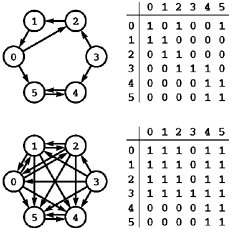
\includegraphics[scale=.7]{informatika/teoreticka_informatika/obrazky/tranzuzaver.png}
    \caption{Tranzitivn� uz�v�r grafu (zdroj: http://zorro.fme.vutbr.cz/graphs/foil36.html)}
  \end{center}
\end{figure}

\begin{e}{Pozn�mka}{0}{0}
  Plat�, �e matice dosa�itelnosti v grafu $G$ = matice sousednosti tranzitivn�ho
  uz�v�ru grafu $G$.
\end{e}

\begin{obecne}{Algoritmus}
Z ka�d�ho vrcholu vypustit DFS (Depth-first search~-- prohled�v�n� do hloubky), do spole�n� matice zaznamen�vat dosa�en� vrcholy (��dek odpov�d� vrcholu, sloupce vrchol�m, kter� jsou z n�ho dosa�iteln�) -- slo�itost $O(n(n+m))$.
\end{obecne}

\begin{obecne}{Warshall�v algoritmus}
Iterativn� konstrukce matice dosa�itelnosti, postupn� po��t� matice $W_k$, kde $w^{[k]}_{i, j} = 1$, pokud mezi vrcholy $i$ a $j$ existuje cesta, jej� v�echny vnit�n� vrcholy jsou mezi vrcholy $1\dots k$.

Z matice $W_k$ lze spo��tat matici $W^{[k+1]}: W^{[k+1]}_{i,j} = W^{[k]}_{i,j}  || (W^{[k]}_{i,k+1} \&\& W^{[k]}_{k+1,j})$ -- bu� vede mezi vrcholy $i, j$ cesta, kter� nepou�ije vrchol $k+1$, nebo takov�, kter� ho pou�ije -- v tom p��pad� ale mus� v�st cesty mezi vrcholy $i,k+1$ a $k+1,j$, kter� pou��vaj� pouze vrcholy $1\dots k$, jejich spojen�m je cesta mezi vrcholy $i,j$

Matice $W^1$ je matice incidence p�vodn�ho grafu.

Pseudok�d (vstup: I -- matice incidence, $[0,1]^{n\times n}$):
\begin{verbatim}
Procedure Warshall(I)
W:= I;
for k:=1 to n
begin
  for i:=1 to n
  begin
    for j:=1 to n
\end{verbatim}
      $w_{i,j} = w_{i,j} || (w_{i,k} \&\& w_{k,j})$
\begin{verbatim}
  end
end 
return W;
\end{verbatim}

Slo�itost algoritmu je jasn� $O(n^3)$ (pot�ebuje $2n^3$ bitov�ch operac�), co� m��e b�t lep�� pro grafy s hodn� hranami (po�et hran se bl�� $n^2$), ne� slo�itost $n*DFS$ ( $n*(n + m) \approx n * (n + n^2) = n^2 + n^3$ )

\end{obecne}

TODO: je�t� n�co?

\subsection{Algoritmy vyhled�v�n� v textu}
Toto s� len ve�mi stru�n� v��ahy z wikipedie. Aktu�lne s� tu len preto, aby si �lovek r�chlo vybavil, o �om tie algoritmy s� :-)

\subsubsection*{Rabin-Karp}
Umo��uje vyh�ad�vanie viacer�ch re�azcov v texte naraz - u�ito�n� napr. na h�adanie plagi�tov. Z�kladnou my�lienkou je vyh�ad�vanie v texte pomocou hashov (rolling hashes - idea je \texttt{s[i+1..i+m] = s[i..i+m-1] - s[i] + s[i+m]})...

Algoritmus pre vyh�ad�vanie jedn�ho re�azca:
\begin{verbatim}
 1 function RabinKarp(string s[1..n], string sub[1..m])
 2     hsub := hash(sub[1..m])
 3     hs := hash(s[1..m])
 4     for i from 1 to n-m+1
 5         if hs = hsub
 6             if s[i..i+m-1] = sub
 7                 return i
 8         hs := hash(s[i+1..i+m])
 9     return not found
\end{verbatim}

Najhor�ia zlo�itos� je $\Omega(mn)$. Pri vyh�ad�van� viacer�ch re�azcov len spo��tame hashe v�ek�ch h�adan�ch stringov a pri n�jden� niektor�ho z hashov pr�slu�n� re�azec porovn�me s textom... Ostatn� algoritmy spotrebuj� �as $O(n)$ na n�jdenie 1 re�azca a teda $O(nk)$ na vyh�adanie $k$ re�azcov. Naproti tomu tento algoritmus m� o�ak�van� zlo�itos� $O(n+k)$ - preto�e vyh�ad�vanie v hashovacej tabu�ke, �i je hash podre�azca textu rovn� hashu niektor�ho z h�adan�ho re�azcov, trv� $O(1)$.

\subsubsection*{Aho-Corasick}

Dok�e vyh�ad�va� viacero re�azcov naraz - pou��va na to trie-like �trukt�ru (kone�n� automat), ktor� obsahuje nasleduj�ce \uv{prvky}:
\begin{penumerate}
	\item kone�n� mno�ina $Q$ - stavy
	\item kone�n� abeceda $A$
	\item transition funkcia $g$: $Q \times A \rightarrow Q + \{fail\}$
	\item failure funkcia $h$: $Q \rightarrow Q + \{fail\}$. $h(q)=q'$ pr�ve vtedy ke� spomedzi v�etk�ch stavov Q d�va $q'$ najdlh�� suffix z $path(q)$.
	\item kone�n� mno�ina $F$ - koncov� stavy
\end{penumerate}

Pr�klad \uv{hotov�ho} automatu pre slov� P=\{ab, ba, babb, bb\}:

\par\begin{center}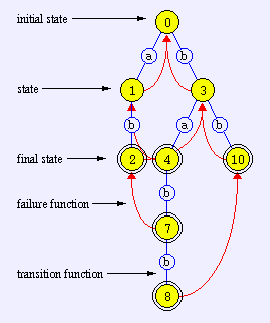
\includegraphics[width=8cm]{informatika/algoritmy_a_ds/obrazky/ahocorasick-automatron.png}\end{center}

Zlo�itos� vyh�ad�vania je line�rna vzh�adom k d�ke textu a po�tu n�jden�ch \uv{slov} (pozn.: ten m��e by� a� kvadradick� - slovn�k a, aa, aaa, aaaa; re�azec aaaa). Trie �trukt�ru je mo�n� vyrobi� raz a potom pou��va� po�as vyh�ad�vania - uchov�vame si najdl�� match a pou��vame suffix odkazy (aby sme udr�ali linearitu v�po�tu).

V�stavba stromu se provede prost�m za�azov�n�m slov do trie-stromu podle prefix�. Na t�to struktu�e je potom mo�n� v line�rn�m �ase (vzhledem k po�tu znak� hledan�ch slov) p�edpo��tat hodnoty failure funkce: automat v�dy pust�me na sufix aktu�ln� zkou�en�ho slova, bez prvn�ho znaku. D�ky tomu, �e pr�b�n� ukl�d�me hodnoty nalezen�ch slov, pro ka�d� p�smeno provede max. 2 kroky (postup vp�ed a ulo�en� hodnoty, kam bych spadnul).


\subsubsection*{Knuth-Morris-Pratt}

Obdoba Aho-Corasick, ale h�ad� len jedno slovo. Samozrejme nie je potrebn� dopredn� funkcia (v�dy iba nasleduj�ci znak), pou��va sa \uv{partial match} tabu�ka (failure funkcia).

\begin{verbatim}
algorithm kmp_search:
    input:
        S (the text to be searched)
        W (the word sought)

    m = 0 (the beginning of the current match in S)
    i = 0 (the position of the current character in W)
    an array of integers, T (the table, computed elsewhere)

    while m + i is less than the length of S, do:
        if W[i] = S[m + i],
            i = i + 1
            if i equals the length of W,
                return m
        otherwise,
            m = m + i - T[i],
            if i is greater than 0,
                i = T[i]

    (if we reach here, we have searched all of S unsuccessfully)
    return the length of S
\end{verbatim}

Zlo�itos� algoritmu je je $O(k)$ (k je d�ka S) - cyklus je vykonan� najviac $2k$ kr�t.

Algoritmus na v�robu tabu�ky:
\begin{verbatim}
algorithm kmp_table:
    input:
        W (the word to be analyzed)
        T (the table to be filled)

    i = 2 (the current position we are computing in T)
    j = 0 (the zero-based index in W of the next
           character of the current candidate substring)

    (the first few values are fixed but different
          from what the algorithm might suggest)
    let T[0] = -1
    T[1] = 0

    while i is less than the length of W, do:
        (first case: the substring continues)
        if W[i - 1] = W[j],
            T[i] = j + 1
            i = i + 1
            j = j + 1

        (second case: it doesn't, but we can fall back)
        otherwise, if j > 0,
            j = T[j]

        (third case: we have run out of candidates. Note j = 0)
        otherwise,
            T[i] = 0
            i = i + 1
\end{verbatim}


Zlo�itos� tohoto algoritmu je $O(n)$ (n je d�ka W) - cyklus skon�� najviac po $2n$ iter�ci�ch.

\subsection{Algebraick� algoritmy}

\subsubsection*{Diskr�tn� Fourierova Transformace (DFT)}

Diskr�tn� Fourierova transformace se pou��v�, chceme-li zachytit hodnotu (p�epokl�dejme, �e $2\pi$-periodick�) funkce na intervalu $[-\pi,\pi]$ v n�jak�ch $n$ bodech. To je dobr� nap�. pro vzorkov�n� elektrick�ho nebo zvukov�ho sign�lu a jin� operace. Pro n�jakou funkci n�m tak sta�� zn�t vektor dimenze $n$ (a $n$ je po�et vzork� na $2\pi$).

Je to zalo�eno na Fourierov�ch �ad�ch -- d� se uk�zat, �e funkce $1$, $\cos kx$ a $\sin kx$ pro $k\geq 1$ tvo�� ortogon�ln� b�zi prostoru spojit�ch funkc� na intervalu $[-\pi,\pi]$. Proto�e pot�ebujeme zn�t jenom kone�n� po�et vzork�, sta�� n�m jen kone�n� podprostor s kone�nou b�z�. M�me-li rozklad n�jak� $2\pi$-periodick� funkce do Fourierovy �ady $f(x)= c + \sum_{k=1}^\infty a_k \sin k x + \sum_{k=1}^\infty b_k \cos k x$, d� se jednodu�e uk�zat, �e pro hodnoty v bodech $-\pi,-\pi + \frac{\pi}{n}, -\pi + 2\frac{\pi}{n}, \dots, -\pi + (n-1)\frac{\pi}{n}$ sta�� sumy do $\frac{n}{2}-1$ pro sinusov� �ady a $\frac{n}{2}$ pro kosinov� -- vy��� koeficienty v takov�ch bodech jsou nulov�. Tak�e $n$ hodnot funkce $f$ na intervalu $[-\pi,\pi]$ lze reprezentovat vektorem $n$ ��sel v b�zi $1,\cos x,\dots,\cos \frac{n}{2}x,\sin x,\dots,\sin(\frac{n}{2}-1)x$. 

Jednodu�eji to lze uk�zat v komplexn�ch ��slech -- je zn�mo, �e 
$$e^{ix} = \cos x+ i\cdot\sin x$$
tak�e vektor hodnot funkce lze ekvivalentn� reprezentovat v b�zi $e^{i\cdot 2\pi\frac{k}{n}},\ k\in\{0,\dots,n\}$, nebo� v�echny vektory p�vodn� b�ze lze zapsat jako line�rn� kombinace vektor� nov� b�ze. Definujeme hodnotu
$$\omega := e^{i\cdot 2\pi\frac{1}{n}} \textrm{ (a to je vlastn� \uv{n�co jako} }\sqrt[n]{1}\textrm{)}$$
vid�me, �e $\omega^k$ je $n$-periodick� funkce, tak�e nez�le�� na hranic�ch sumace ($-\frac{n}{2}+1,\dots,\frac{n}{2}$ je ekvivalentn� $0,\dots,n-1$). 
Potom se posloupnost $n$ komplexn�ch ��sel $\alpha_0, \dots, \alpha_{n-1}$ (nap�. hodnot na�� funkce v bodech $-\pi + \frac{2\pi k}{n},\ k\in\{0,\dots,n-1\}$) transformuje na posloupnost $n$ komplexn�ch ��sel $A_0, \dots, A_{n-1}$ (do b�ze $\omega^i,\ i\in\{0,\dots,n-1\}$) pou�it�m vzore�ku:
$$A_j = \sum_{k=0}^{n-1} \alpha_k \omega^{kj}  \;\;\;\;\; j = 0, \dots, n-1$$
Tento p�evod ozna�ujeme jako \emph{diskr�tn� Fourierovu transformaci}.

\emph{Inverzn� diskr�tn� Fourierova transformace} je opa�n� probl�m -- z $n$ Fourierov�ch koeficient� $A_k$ chceme zp�tn� vypo��tat hodnoty funkce $\alpha_k$ v bodech $-\pi + \frac{2\pi k}{n},\ k\in\{0,\dots,n-1$. Plat�:

$$\alpha_j = \frac{1}{n}\sum_{k=0}^{n-1} A_k \omega^{-kj}  \;\;\;\;\; j = 0, \dots, n-1$$

\medskip
\begin{e}{D�kaz}{0}{0}
Definujeme matici $W: W_{p,q}=\omega^{pq}$, potom $A = W\alpha$ (vektorov�), tak�e $a = W^{-1}A$. Definujeme $W': W'_{p,q}=\omega^{-pq}$ a dok�eme, �e $W\cdot W'= n\cdot I_n$. M�me
$$(W\cdot W')_{p,q} = \sum_{s=0}^{n-1} W_{p,s}\cdot W'_{s,q} = \sum_{s=0}^{n-1} \omega^{(p-q)\cdot s}$$
a potom pro
\begin{pitemize}
    \item $p = q$ plat� $\sum_{s=0}^{n-1}\omega^{(p-q)\cdot s} = \sum_{s=0}^{n-1}\omega^0 = \sum_{s=0}^{n-1} 1 = n$
    \item $p\neq q$ definujeme
    $$Q:= \omega^{p-q}$$
    a dostaneme geometrickou posloupnost $Q^0 + Q^1 +\dots +Q^{n-1}$, pro jej� sou�et prvn�ch $n$ �len� plat� vzorec
    $$ \sum_{s=0}^{n-1} Q^s = Q^0 \frac{Q^{n-1+1} - 1}{Q-1} = 1\frac{1-1}{Q-1}= 0 $$
\end{pitemize}
\end{e}


\begin{e}{Algoritmus}{0}{Fast Fourier transform (FFT)}
Fast Fourier transform je algoritmus pro po��t�n� diskr�tn� Fourierovy transformace vektor� rozm�ru $n=2^k$ v �ase $\Theta(n\log n)$. M�m-li matici Fourierov�ch koeficient� $W, W_{p,q} = \alpha_q \omega^{pq}$, mohu ji rozd�lit na lich� a sud� sloupce, u sud�ch vyj�d�it $\omega^q$ a pro spodn� polovinu ��dek (se sumami jdouc�mi po dvou) mohu sn�it exponent u $\omega$ o $n/2$ (d�ky periodicit�) a vyjdou stejn� ��sla:
\begin{align*}
    A_j &= \sum_{k=0}^{n-1} \alpha_k \omega^{kj}\ &j\in\{0,\dots,n-1\}\\
    \\
    A_j &= \sum_{k=0}^{\frac{n}{2}-1} \alpha_{2k}\omega^{2kj} + \omega^j \sum_{k=0}^{\frac{n}{2}-1} \alpha_{2k+1}\omega^{2kj}\ &j\in\{0,\dots,\frac{n}{2}-1\}\\    
    A_{j+\frac{n}{2}} &= \sum_{k=0}^{\frac{n}{2}-1} \alpha_{2k}\omega^{2k(j+\frac{n}{2})} + \omega^{(j+\frac{n}{2})} \sum_{k=0}^{\frac{n}{2}-1} \alpha_{2k+1}\omega^{2k(j+\frac{n}{2})}\ &j\in\{0,\dots,\frac{n}{2}-1\}\\
\end{align*}

\textit{Pozn�mka: pro rychl� a jednoduch� pochopen� t�ch blekt� co jsem tu napsal doporu�uji Ku�er�v program Algovision}\\ \texttt{http://kam.mff.cuni.cz/\~{}ludek/AlgovisionPage.html} \\ \textit{DFT je tam n�zorn� a p�ehledn� uk�zan�.}
\end{e}

TODO: Souvisej�c� obecn� \uv{v�ci} o Fourierov� transofrmaci, pou�it� p�i spektr�ln� anal�ze (Nyquist-Shannon sampling theorem), datov� kompresi (Diskr�tn� kosinov� transformace), n�soben� polynom� (+n�soben� velk�ch integer�).

\subsubsection*{Euklid�v algoritmus}

Euklid�v algoritmus je postup (algoritmus), kter�m lze ur�it nejv�t��ho spole�n�ho d�litele dvou p�irozen�ch ��sel, tzn. nejvy��� ��slo takov�, �e beze zbytku d�l� ob� ��sla.

Algoritmus (pomoc� rekurze):
\begin{verbatim}
function gcd(a, b)
    if b = 0 return a
    else return gcd(b, a mod b)
\end{verbatim}

Algoritmus (pomoc� iterace):
\begin{verbatim}
function gcd(a, b)
    while b <> 0
        t := b
        b := a mod b
        a := t
    return a
\end{verbatim}

Algoritmus (jednoduch� ale neefektivn�):
\begin{verbatim}
function gcd(a, b)
    while b <> 0
        if a > b
            a := a - b
        else
            b := b - a
    return a
\end{verbatim}

Doba prov�d�n� programu je z�visl� na po�tu pr�chod� hlavn� smy�kou. Ten je maxim�ln� tehdy, jsou-li po��te�n� hodnoty u a v rovn� dv�ma po sob� jdouc�m �len�m Fibonacciho posloupnosti. Maxim�ln� po�et proveden�ch opakov�n� je tedy $\log_\phi (3-\phi)v \approx 4{,}785 \log v + 0{,}6273 = O(\log v)$. Pr�m�rn� po�et krok� pak je o n�co ni���, p�ibli�n� $\frac{12 \ln 2}{\pi^2}\log v \approx 1{,}9405 \log v = O(\log v)$.
\\\\
\begin{e}{Report}{0}{Skopal} DFT
\end{e}

\subsection{Z�klady kryptografie, RSA\sout{, DES}}

(nejsou zde uvedeny p��klady symetrick�ch �ifer, pro z�jemce vesel� komiks o AES -- \url{http://www.moserware.com/2009/09/stick-figure-guide-to-advanced.html} :))

\subsubsection*{Z�klady kryptografie\footnote{sestaveno podle vrazedneho zkouseni Jaghobem}} 
\begin{e}{Definice}{1}{Kryptografick� syst�m}
Prostor otev�en�ch zpr�v $M$, �ifrovan�ch zpr�v $C$, �ifrovac�ch a de�ifrovac�ch kl��� $K$ a $K'$. Efektivn� generov�n� kl���
                        $G:N\to K\times K'$, �ifrov�n� $E:M\times K\to C$, de�ifrov�n� $D:C\times K'\to M$.
\begin{pitemize}
  \item \textbf{Symetrick�} (sd�len� kl�� $k_e = k_d$) rychl�, kr�tk� kl��e, potreba menit klice a bezpecne si je vymenit
  \item\textbf{Asymetrick�} (ve�ejn� kl�� $k_e \neq k_d$) delsi klice a pomalejsi nez symetrick�, neni pot�eba tajn� v�m�na, neni pot�eba tak �asto m�nit kl��e 
\end{pitemize}                  
\end{e}

\begin{e}{Definice}{0}{Nahodn� gener�tory}
Pou��vaj� se pro generov�n� kl��� pro �ifry (nap� RSA) a v proudov�ch �ifr�ch.
\begin{pitemize}
  \item\textbf{HW} za��zen� �asto zalo�en� na jevech generuj�c�ch statisticky n�hodn� "�umov�" sign�ly, nap��klad z tepeln�ho �umu polovodi�e.
  \item\textbf{SW} jsou zalo�eny na pozorov�n� jev� v po��ta�i z hlediska programu n�hodn�ch, �asto z u�ivatelsk�ho vstupu (nap�. PuTTYgen pou��v� pro generov�n� RSA kl��e p�ej�zd�n� my��). 
  \item\textbf{Pseudon�hodn�} jsou deterministick� programy generuj�c� posloupnost ��sel pokud mo�no nerozli�itelnou od n�hodn�.
        \begin{pitemize}
                \item p�. kongruen�n� gener�tor: $X_{n+1} = ( a X_n + c ) \mod m$ 
                \item pou��vaj� se v proudov�ch �ifr�ch
        \end{pitemize}  
\end{pitemize} 
\end{e}

\begin{e}{Definice}{0}{Hashovaci funkce}
Funkci $h:U\rightarrow\{0,1,\dots,m-1\}$ naz�v�me \textbf{ha�ovac� funkc�}.\footnote{viz ot�zku Ha�ov�n�}
\\\\
\textbf{Po�adavky:}
\begin{pitemize}
  \item Rovnom�rn� a n�hodn� rozlo�en� hodnot
  \item Odolnost na kolize (v�po�etn� slo�it� naj�t pro $x\neq x$ $h(x)=h(y)$) 
  \item Jednosm�rn� funkce (v�po�etn� slo�it� naj�t $y$ k $x$ pro $h(x)=y$)     
  \item Efektivn� algoritmus
\end{pitemize} 
\textbf{Vyu�it�:}
CRC (kontroln� sou�et), ukl�d�n� hesel (MD5,SHA) ...      

\end{e}

\begin{e}{Definice}{0}{Model utocnika podle Doleva a Yao}
\begin{pitemize}
  \item M��e z�skat libovolnou zpr�vu putuj�c� po s�ti
  \item Je pr�voplatn�m u�ivatelem s�t� a tud� m��e zah�jit komunikaci s jin�m u�ivatelem
  \item M��e se st�t p��jemcem zpr�v kohokoliv
  \item M��e zas�lat zpr�vy komukoliv zosobn�n�m se za jin�ho u�ivatele
  \item Neumi rozume resit NP-uplne problemy (ani slozitejsi)\footnote{tzn. i slab��: Nem��e odhadnout n�hodn� ��slo z dostate�n� velk�ho prostoru}   
  \item Bez spr�vn�ho kl��e nem��e nal�zt zpr�vu k �ifrovan� zpr�v� a nem��e vytvo�it platnou �ifrovanou zpr�vu z dan� zpr�vy, v�e vzhledem k n�jak�mu �ifrovac�mu algoritmu 
\end{pitemize}  
\end{e}

\begin{e}{Definice}{0}{Cile utoku}
        \begin{description}
                \item\textbf{d�v�rnost dat} u�ivatel m��e ur�it kdo m� data vid�t, a syst�m skute�n� dovol� pracovat s daty pouze povolen�m u�ivatel�m
                \item\textbf{celistvost dat} mo�nost podstr�en� fale�n�ch dat
                \item\textbf{dostupnost syst�mu} \emph{DoS (Denial of Service)}
        \end{description}
\end{e}

\begin{e}{P��klad}{0}{0}
Ukazku pouziti nejakeho sifrovaciho protokolu (zvolil jsem kombinace symetricka sifra sifrovani, asymetricka predani klicu k symetricke).
\\\\TODO
\end{e}
\begin{e}{Definice}{0}{protokol Diffie-Hellman}
\begin{pitemize} 
\item Diffie-Hellman v�mena kl�cu je kryptografick� protokol, kter� umo�nuje nav�zat bezpecn� spojen�. Pro bezpecn� spojen� je potreba si vymenit kl�c k symetrick� �ifre pres je�te nezabezpecen� kan�l. Pr�ve tento protokol to umo�nuje ani� by byl kl�c jednodu�e posl�n v otevren� forme.
\item Alice si vymysl� velk� prvoc�slo $p$, gener�tor $g$ kone�n� grupy $G=(Z^*_p,\cdot)$
a $a\in[1,p-1)$ vypocte A po�le Bobovi [g,p,A], Bob vypocte B a po�le ho Alici oba si vypoc�taj� K $\Rightarrow$ muzou zacit symetricky sifrovanou komunikaci
\end{pitemize}

\begin{figure}
  \begin{center}
    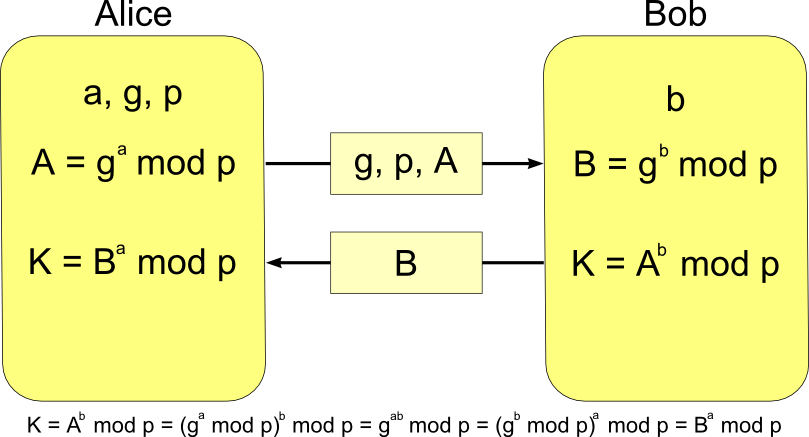
\includegraphics[width=10cm]{informatika/siete_a_bezpecnost/obrazky/dh-system.png}
    \caption{D-H protokol}
  \end{center}
\end{figure}

\begin{pitemize}
\item Puvodne nezabezpecoval autentifikaci ucastniku = nachylny k utoku man-in-the-middle. Man-in-the-middle muze vytvorit komunikaci s dvema ruznymi Diffie-Hellman klici, jeden s Alici a druhej s Bobem, a pak se tvarit jako Alice k Bobovi a obracene, treba pomoci dekodovani a rekodovani zprav mezi nimi. Nejaka metoda autentifikace mezi temito osobami je nutna.
\item Probl�mu nalezen� c�sla  a  ze znalosti ga  mod  p  se r�k� probl�m diskr�tn�ho logaritmu.  Tento probl�m je st�le pova�ov�n za velmi obt�n�. \end{pitemize} 

\end{e}

\subsubsection*{RSA (Rivest-Shamir-Adleman)}
Asymetrick� �ifra (r�zn� kl��e pro �ifrov�n� a de�ifrov�n�), pou�iteln� jako �ifra s�ve�ejn�m kl��em. Kryptosch�ma je zalo�eno na Eulerove formuli.
\\\\
Alice a Bob se verejne dohodnou na hranici $N$ a chtej� si vymenovat tajn� zpr�vy $0 \leq m<N$.
\textbf{Inicializace:}
\begin{penumerate}
        \item vybrat dv� dostate�n� velk� prvo��sla $p$, $q$ tak aby $n= p\cdot q < N$
        \item Alice spo��t� $\varphi(n) = (p-1)\cdot (q-1)$\\ 
        (Eulerova funkce $\varphi(n)$ je po�et ��sel men��ch ne� $n$, kter� jsou s $n$ nesoud�ln�)
        \item vybrat $e$ takov�, �e $1 < e < \varphi(n)$ a $e$ je nesoud�ln� s $\varphi(n)$\\ -- dvojice ($n,e$) bude \emph{ve�ejn� kl�� (public key)}
        \item vybrat $d$ tak, aby 
                $$d\cdot e \equiv 1 \mod \varphi(n)$$ 
                takov� $d$ lze naj�t roz���en�m euklidov�m algoritmem\\
                -- dvojice ($n,d$) bude \emph{de�ifrovac� kl�� (private key)}
\end{penumerate}

\textbf{�ifrov�n�:}
\begin{penumerate}
        \item Alice pos�l� public key Bobovi (��sla $n$ a $e$), nech�v� si private key
        \item Bob chce Alici poslat zpr�vu $m$ tak spo��t� :
                $$c = m^e \mod n$$
        \item Bob ode�le $c$ Alici
\end{penumerate}

\textbf{De�ifrov�n�:}
\begin{penumerate}
\item Alice p�ijala $c$
\item Spo��t�:
        $$m = c^d \mod n$$
\end{penumerate}

�ifra (to, �e to v�bec funguje, tedy, �e $m = (m^e)^d$) se op�r� o n�kolik netrivi�ln�ch v�t algebry...
\begin{pitemize}
\item Pro re�ln� pou�it� c�sla pribli�ne 100 a� 200 bitu. Kl�c e vol�me jako prvoc�slo vet�� ne� $(p - 1)$ a $(q � 1)$. Hranice bezpecnosti pro modul n je $N$ = 1024 bitu, rozumn� 1500 bitu, l�pe 2048
\item Nen� zn�ma metoda vedouc� k rozbit� tohoto algoritmu
\item Slabost� je hypotetick� mo�nost vytvorit elektronick� podpis zpr�vy bez znalosti de�ifrovac�ho kl�ce na z�klade zachycen� vhodn�ch predchoz�ch za�ifrovan�ch zpr�v.
\item nap��klad SSH protokol pou��v� RSA kl��e
\end{pitemize}

\begin{e}{Report}{0}{Skopal} RSA, DES (tady cht�l Skopal konkr�tn� vzore�ky, jak funguje symetrick� �ifra nebo �ifrov�n� s v��ejn�m kl��em ho nez�j�malo)
\end{e}

\begin{e}{Report}{0}{Yaghob}
Vedom si nebezpecnosti situace nabidl jsem p. Yaghobovi "sestaveni nakupniho kosiku". Povedel jsem, ze by se k tematu dala povedet hromada veci, tak jestli bychom se mohli domluvit na podmnozine ktera jej zajima, at zbytecne neplnim papir. Souhlasil nacez jsem mu nabidl hromadu vice ci mene souvisejicich veci, pridal par hodne vlastnich.
\\\\Nechtel: S-Box, RSA,DES ani zadnou konkretni sifru, konkretni metody utoku, obranu proti utokum, pravidla pro volbu dobreho hesla, steganografii, proudove sifry,historii...
\\\\Chtel:

    Formalne popsat kryptograficky system - bacha! tady bylo videt, ze jde o klicovy pojem, kdyz ho clovek neformuluje - tak (nejspis) konci.

    Nahodne generatory + vlastnosti, ktere od nich chceme + zhruba algoritmicky princip (an = (an-1*b+c) mod d)) + kde se pouziji (generovani klicu)
    
    Hashovaci funkce + vlastnosti, ktere od nich chceme, kde se pouziji (crc, neukladat hesla v plaintextu, ...)
    
    Model utocnika podle Doleva a Yao (pozor! v materialech napsano: neumi uhodnout nah.cislo z dost velke mnoziny, spravne je obecnejsi: Neumi rozume resit NP-uplne problemy (ani slozitejsi (: )).
    
    Cile utoku
    
    Ukazku pouziti nejakeho sifrovaciho protokolu (zvolil jsem kombinace symetricka sifra sifrovani, asymetricka predani klicu k symetricke).
    
    Vymenu klicu a-la Diffie Hellman
    
    Pokud jsem neco nevedel, dostal jsem cas na premysleni, pripadne jemne natuknuti. Veci chtel hodne formalne.
    
    Nemit Ochranu informace I a II + vlastni zajem o oblast, tak certain doom!
\end{e}



\section{Databáze}
\begin{pozadavky}
\begin{pitemize}
\item Podstata a architektury DB systémů
\item Konceptuální, logická a fyzická úroveň pohledů na data
\item Algoritmy návrhu schémat relací, normální formy, referenční integrita
\item Transakční zpracování, vlastnosti transakcí, uzamykací protokoly, zablokování
\item ER-diagramy, metody návrhů IS
\item SQL
\item Indexy, triggery, uložené procedury, uživatelé, uživatelská práva
\item Vícevrstevné architektury
\item Vazba databází na internetové technologie
\item Organizace dat na vnější paměti, B-stromy a jejich varianty.
\end{pitemize}
\end{pozadavky}
\subsection{Podstata a architektury DB system�}

Zdroje: Wikipedie, slidy Dr. T. Skopala k Datab�zov�m syst�m�m
\bigskip

\begin{e}{Definice}{0}{Datab�ze}
Datab�ze je logicky uspo��dan� (integrovan�) kolekce navz�jem souvisej�c�ch dat. Je sebevysv�tluj�c�, proto�e data jsou uchov�v�na spole�n� s�popisy, zn�m�mi jako metadata (tak� sch�ma datab�ze). Data jsou ukl�d�na tak, aby na nich bylo mo�n� prov�d�t strojov� dotazy -- z�skat pro n�jak� parametry vyhovuj�c� podmno�inu z�znam�.

N�kdy se slovem \uv{datab�ze} mysl� obecn� cel� datab�zov� syst�m.
\end{e}

\begin{e}{Definice}{0}{Syst�m ��zen� b�ze dat}
Syst�m ��zen� b�ze dat (S�BD, anglicky database management system, DBMS) je obecn� softwarov� syst�m, kter� ��d� sd�len� p��stup k�datab�zi, a poskytuje mechanismy, pom�haj�c� zajistit bezpe�nost a integritu ulo�en�ch dat. Spravuje datab�zi a zaji��uje prov�d�n� dotaz�.
\end{e}

\begin{e}{Definice}{0}{Datab�zov� syst�m}
Datab�zov�m syst�mem rozum�me trojici, sest�vaj�c� z:
\begin{pitemize}
    \item datab�ze
    \item syst�mu ��zen� b�ze dat
    \item chud�ka admina
\end{pitemize}
\end{e}

\begin{obecne}{Smysl datab�z�}
Hlavn�m smyslem datab�ze je schra�ovat datov� z�znamy a informace za ��elem:
\begin{pitemize}
    \item sd�len� dat v�ce u�ivateli,
    \item zaji�t�n� unifikovan�ho rozhran� a jazyk� definice dat a manipulace s daty,
    \item znovuvyu�itelnosti dat,
    \item bezespornosti dat a
    \item sn�en� objemu dat (odstran�n� redundance).
\end{pitemize}
\end{obecne}

\subsubsection*{Datab�zov� modely}

\begin{e}{Definice}{0}{sch�ma, model}
Typicky pro ka�dou datab�zi existuje struktur�ln� popis druh� dat v n� udr�ovan�ch, ten naz�v�me \emph{sch�ma}. Sch�ma popisuje objekty reprezentovan� v datab�zi a vztahy mezi nimi. Je n�kolik mo�n�ch zp�sob� organizace sch�mat (modelov�n� datab�zov� struktury), zn�m�ch jako \emph{modely}. V modelu jde nejen o zp�sob strukturov�n� dat, definuje se tak� sada operac� nad daty provediteln�. Rela�n� model nap��klad definuje operace jako \uv{select} nebo \uv{join}. I kdy� tyto operace se nemusej� p��mo vyskytovat v dotazovac�m jazyce, tvo�� z�klad, na kter�m je jazyk postaven. Nejd�le�it�j�� modely v t�to sekci pop�eme.
\end{e}

\begin{e}{Pozn�mka}{0}{0}
V�t�ina datab�zov�ch syst�m� je zalo�ena na jednom konkr�tn�m modelu, ale ��m d�l �ast�j�� je podpora v�ce p��stup�. Pro ka�d� logick� model existuje v�ce fyzick�ch p��stup� implementace a v�t�ina syst�m� dovol� u�ivateli n�jakou �rove� jejich kontroly a �prav, proto�e toto m� velk� vliv na v�kon syst�mu. P��kladem nech� jsou indexy, provozovan� nad rela�n�m modelem.
\end{e}

\begin{obecne}{\uv{Ploch�} model}
Toto sice nevyhovuje �pln� definici modelu, p�esto se jako trivi�ln� p��pad uv�d�. P�edstavuje jedinou dvoudimension�ln� tabulku, kde data v jednom sloupci jsou pova�ov�na za popis stejn� vlastnosti (tak�e maj� podobn� hodnoty) a data v jednom ��dku se uva�uj� jako popis jedin�ho objektu.
\end{obecne}

\begin{obecne}{Rela�n� model}
Rela�n� model je zalo�en na predik�tov� logice a teorii mno�in. V�t�ina fyzicky implementovan�ch datab�zov�ch syst�m� ve skute�nosti pou��v� jen aproximaci matematicky definovan�ho rela�n�ho modelu. Jeho z�kladem jsou \emph{relace} (dvoudimension�ln� tabulky), \emph{atributy} (jejich pojmenovan� sloupce) a \emph{dom�ny} (mno�iny hodnot, kter� se ve sloupc�ch m��ou objevit). Hlavn� datovou strukturou je tabulka, kde se nach�z� informace o n�jak� konkr�tn�  t��d� entit. Ka�d� entita t� t��dy je potom reprezentov�na ��dkem v tabulce -- $n$-tic� atribut�.

V�echny relace (tj. tabulky) mus� spl�ovat z�kladn� pravidla -- po�ad� sloupc� nesm� hr�t roli, v tabulce se nesm� vyskytovat identick� ��dky a ka�d� ��dek mus� obsahovat jen jednu hodnotu pro ka�d� sv�j atribut. Rela�n� datab�ze obsahuje v�ce tabulek, mezi kter�mi lze popisovat vztahy (v�ech r�zn�ch kardinalit, tj. $1:1$, $1:n$ apod.). Vztahy vznikaj� i implicitn� nap�. ulo�en�m stejn� hodnoty jednoho atributu do dvou ��dk� v tabulce. K tabulk�m lze p�idat informaci o tom, kter� podmno�ina atribut� funguje jako \emph{kl��}, tj. unik�tn� identifikuje ka�d� ��dek, n�kter� z kl��� m��e b�t ozna�en jako prim�rn�. N�kter� kl��e m��ou m�t n�jak� vztah k vn�j��mu sv�tu, jin� jsou jen pro vnit�n� pot�eby sch�matu datab�ze (generovan� ID).
\end{obecne}

\begin{obecne}{Hierarchick� model}
V hierarchick�m modelu jsou data organizov�na do stromov� struktury -- ka�d� uzel m� odkaz na nad��zen� (k popisu hierarchie) a set��d�n� pole z�znam� na stejn� �rovni. Tyto struktury byly pou��v�ny ve star�ch mainframeov�ch datab�z�ch, nyn� je m��eme vid�t nap� ve struktu�e XML dokument�. Dovoluj� vztahy $1:N$ mezi dv�ma druhy dat, co� je velice efektivn� k popisu r�zn�ch re�ln�ch vztah� (obsahy, �azen� odstavc� textu, t��d�n� informace). Nev�hodou je ale nutnost zn�t celou cestu k z�znamu ve struktu�e a neschopnost syst�mu reprezentovat redundance v datech (strom nem� cykly).
\end{obecne}

\begin{obecne}{S�ov� model}
S�ov� model organizuje data pomoc� dvou hlavn�ch prvk�, \emph{z�znam�} a \emph{mno�in}. Z�znamy obsahuj� pole dat, mno�iny definuj� vztahy $1:N$ mezi z�znamy (jeden \emph{vlastn�k}, mnoho \emph{prvk�}). Z�znam m��e b�t vlastn�kem i prvkem v n�kolika r�zn�ch mno�in�ch. Jde vlastn� o variantu hierarchick�ho modelu, proto�e s�ov� model je tak� zalo�en na konceptu v�ce struktur ni��� �rovn� z�visl�ch na struktur�ch �rovn� vy���. U� ale umo��uje reprezentovat i redundantn� data. Operace nad t�mto modelem prob�haj� \uv{naviga�n�m} stylem: program si uchov�v� svoji sou�asnou pozici mezi z�znamy a postupuje podle z�vislost�, ve kter�ch se dan� z�znam n�ch�z�. Z�znamy mohou b�t i vyhled�v�ny podle kl��e. 

Fyzicky jsou v�t�inou mno�iny -- vztahy -- reprezentov�ny p��mo ukazateli na um�st�n� dat na disku, co� zaji��uje vysok� v�kon p�i vyhled�v�n�, ale zvy�uje n�klady na reorganizace. Smysl s�ov� navigace mezi objekty se pou��v� i v objektov�ch modelech.
\end{obecne}

\begin{obecne}{Objektov� model}
Objektov� model je aplikac� p��stup� zn�m�ch z objektov�-orientovan�ho programov�n�. Je zalo�en na sbli�ov�n� programov� aplikace a datab�ze, hlavn� ve smyslu pou�it� datov�ch typ� (objekt�) definovan�ch na jednom m�st�; ty zp��stup�uje k pou�it� v n�jak�m b�n�m programovac�m jazyce. Odstran� se tak nutnost zbyte�n�ch konverz� dat. P�in�� do datab�z� tak� v�ci jako zapouzd�en� nebo polymorfismus. Probl�mem objektov�ch model� je neexistence standard� (nebo sp� produkt�, kter� by je implementovaly).

Kombinac� objektov�ho a rela�n�ho p��stupu vznikaj� \emph{objektov�-rela�n�} datab�ze -- rela�n� datab�ze, dovoluj�c� u�ivateli definovat vlastn� datov� typy a operace na nich. Obsahuj� pak hybrid mezi procedur�ln�m a dotazovac�m programovac�m jazykem.

\end{obecne}


\subsubsection*{Architektury datab�zov�ch syst�m�}

Zdroj: Wiki �VUT (st�tnice na FELu ;-))
\bigskip

Architektury datab�zov�ch syst�m� se obecn� d�l� na 
\begin{pitemize}
    \item \emph{centralizovan�} (kde se datab�ze p�edpokl�d� fyzicky na jednom po��ta�i) a
    \item \emph{distribuovan�},
\end{pitemize}
p��padn� na
\begin{pitemize}
    \item \emph{jednou�ivatelsk�} a
    \item \emph{v�ceu�ivatelsk�}.
\end{pitemize}

\begin{obecne}{Distribuovan� datab�zov� syst�my}
\emph{Distribuovan� syst�m ��zen� b�ze dat} je vlastn� speci�ln�m p��padem obecn�ho distribuovan�ho v�po�etn�ho syst�mu. Jeho implementace zahrnuje fyzick� rozlo�en� dat (v�etn� mo�n�ch replikac� datab�ze) na v�ce po��ta�� -- \emph{uzl�}, p�i�em� jejich popis je integrov�n v glob�ln�m datab�zov�m sch�matu. Data v uzlech mohou b�t zpracov�v�na lok�ln�mi S�BD, komunikace je organizov�na v s�ov�m provozu pomoc� speci�ln�ho softwaru, kter� um� zach�zet s distribuovan�mi daty. Fyzicky se �e�� rozlo�en� do uzl�, sv�zan�ch komunika�n�mi kan�ly, a jeho transparence (neviditelnost -- navenek se m� tv��it jako jednolit� syst�m). Ka�d� uzel v s�ti je s�m o sob� datab�zov� syst�m a z ka�d�ho uzlu lze zp��stupnit data kdekoliv v s�ti.

D�le se d�l� na dva typy:
\begin{pitemize}
    \item Federativn� datab�ze -- neexistuje glob�ln� sch�ma ani centr�ln� ��d�c� autorita, ��zen� je tak� distribuovan�.
    \item Heterogenn� datab�zov� syst�my -- jednotliv� autonomn� S�BD existuj� (vznikly nez�visle na sob�) a jsou integrov�ny, aby spolu mohly komunikovat.
\end{pitemize}

V�hodou oproti centralizovan�m syst�m�m je vy��� efektivita (data mohou b�t ulo�ena bl�zko m�sta nej�ast�j��ho pou��v�n�), zv��en� dostupnost, v�konnost a roz�i�itelnost; nev�hodou z�st�v� probl�m slo�itosti implementace, distribuce ��zen� a ni��� bezpe�nost takov�ch �e�en�.
\end{obecne}

\begin{obecne}{V�ceu�ivatelsk� datab�zov� syst�my}
\emph{V�ceu�ivatelsk�} jsou takov� syst�my, kter� umo��uj� v�cen�sobn� u�ivatelsk� p��stup k dat�m ve stejn�m okam�iku. V d�sledku mo�n�ho sou�asn�ho p��stupu v�ce u�ivatel� je nutn� syst�m zabezpe�it tak, aby i nad�le zaji��oval integritu a konzistenci ulo�en�ch dat. Existuj� obecn� dva mo�n� p��stupy:
\begin{pitemize}
    \item Uzamyk�n� -- D��ve �asto pou��van� metoda zalo�en� na uzamyk�n� aktualizovan�ch z�znam�, v p��pad� masivn�ho vyu�it� aktualiza�n�ch p��kaz� u n� ale m��e doch�zet k zna�n�m prodlev�m. 
    \item Multiversion Concurency Control -- Modern�j�� vyn�lez. Jeho princip spo��v� v tom, �e p�i po�adavku o aktualizaci z�znamu v tabulce je vytvo�ena kopie z�znamu, kter� nen� pro ostatn� u�ivatele a� do proveden�ho commitu viditeln�.
\end{pitemize}
\end{obecne}

\subsection{Konceptualn�, logick� a fyzick� �rove� pohledu na data}

TODO: sjednotit terminologii, snad to popisuje to co tu m� b�t, ale zdroje jsou pochybn� (Wikipedie tady neodv�d� zrovna ide�ln� pr�ci a �VUT Wiki se moc nerozepisuje).

\begin{e}{Definice}{0}{Datov� modelov�n�}
\emph{Datov� modelov�n�} je proces vytvo�en� konkr�tn�ho datov�ho modelu (sch�matu) datab�ze pomoc� aplikace n�jak�ho abstraktn�ho datab�zov�ho modelu. Datov� modelov�n� zahrnuje krom� definice struktury a organizace dat je�t� dal�� implictin� nebo explicitn� omezen� na data do struktury ukl�dan�. 
\end{e}

\begin{obecne}{Vrstvy modelov�n�}
Druhy datov�ch model� mohou b�t t�� typ�, podle t�� r�zn�ch pohled� na datab�ze (t�i \uv{vrstvy}, kter� se navz�jem dopl�uj�):
\begin{pitemize}
    \item konceptu�ln� sch�ma (datov� model) -- nejabstraktn�j��, popisuje v�znam organizace datab�ze -- t��dy entit a jejich vztahy.
    \item logick� sch�ma -- popisuje v�znam konceptu�ln�ho sch�matu z hlediska datab�zov� implementace -- popisy tabulek, programov�ch t��d nebo XML tag� (podle zvolen�ho datab�zov�ho modelu)
    \item fyzick� sch�ma -- nejkonkr�tn�j��, popisuje fyzick� ulo�en� dat a stroje na kter�ch syst�m pob��.
\end{pitemize}
Na tomto rozd�len� je d�le�it� nez�vislost jednotliv�ch vrstev -- tak�e se implementace jedn� z nich m��e zm�nit, ani� by bylo nutn� v�razn� upravovat ostatn� (samoz�ejm� mus� z�stat konzistetn� vzhledem k ostatn�m vrstv�m). B�hem implementace n�jak� datab�zov� aplikace se za��n� vytvo�en�m konceptu�ln�ho sch�matu, pokra�uje jeho up�esn�n� logick�m sch�matem a naknec jeho fyzickou implementac� podle fyzick�ho sch�matu (modelu).
\end{obecne}

\begin{e}{Pozn�mka}{0}{0}
V tomto pohledu (kter� je podle standardu ANSI z r. 1975) jsou datab�zov� modely, popsan� v p�edchoz� sekci, p��klady abstraktn�ch logick�ch datov�ch model�. N�kde je v�ak tato �rove� ozna�ov�na jako \uv{fyzick�} a \uv{jin� logick�} se vt�sn� je�t� mezi ni a konceptu�ln�.
\end{e}


\begin{obecne}{Konceptu�ln� sch�ma}
\emph{Konceptu�ln� sch�ma} (datov� model) popisuje podstatn� objekty (\emph{t��dy entit}, \uv{koncepty}), jejich charakteristiky (\emph{atributy}) a vztahy mezi nimi (asociace mezi dvojicemi t��d entit). Nepopisuje p��mo implementaci v datab�zi, jen v�znam n�jak�ho celku, kter� bude datab�z� p�edstavov�n. Jde o modelov�n� \uv{datov� reality}, z pohledu u�ivatele (analytika, konstrukt�ra datab�ze).

\medskip
\begin{e}{P��klady}{0}{0}
P�r p��klad� vztah� mezi t��dami entit (z Wikipedie):
\begin{pitemize}
    \item Each PERSON may be the vendor in one or more ORDERS.
    \item Each ORDER must be from one and only one PERSON.
    \item PERSON is a sub-type of PARTY. (Meaning that every instance of PERSON is also an instance of PARTY.)
\end{pitemize}
\end{e}
De-facto standardem pro konceptu�ln� datov� modelov�n� jsou \emph{ER-diagramy} (entity-relationship diagramy). Hod� se hlavn� pro \uv{ploch�} form�tovan� data (tak�e t�eba pro objektov� nebo rela�n� datab�ze, ale ne pro XML apod.). Pou��vaj� dva typy \uv{objekt�} -- \emph{entity} (t��dy entit) a \emph{vztahy}. Jde o obdobu UML z objektov�ho programov�n�. P��klad ER-diagramu se vztahem dvou entit je na n�sleduj�c�m obr�zku (popisuje i dal�� vlastnosti -- atributy entit a kardinality vztah�):
\begin{center}
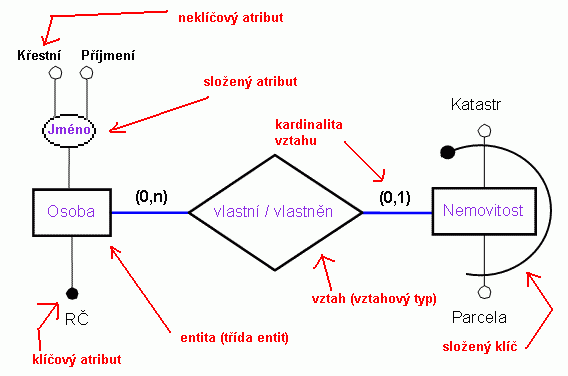
\includegraphics[width=14cm]{informatika/databazy/obrazky/er-schema.png}

(Obr�zek je upraven�, roz���en� a popsan� p��klad ze slid� Dr. T. Skopala k Datab�zov�m syst�m�m)
\end{center}
\end{obecne}

\begin{obecne}{Logick� sch�ma}
\emph{Logick� sch�ma} je datov� model organizace n�jak�ho specifick�ho celku pomoc� jednoho z datab�zov�ch model� -- podle datab�zov�ch model� popsan�ch v p�edchoz� sekci, tj. nap�. pomoc� rela�n�ch tabulek, objektov�ch t��d nebo XML. Svoj� �rovn� abstrakce se nach�z� mezi konceptu�ln�m a fyzick�m sch�matem.
\end{obecne}

\begin{obecne}{Fyzick� sch�ma}
\emph{Fyzick� datov� modely} jsou modely, ktere pou��vaj� databazov� stroje sm�rem k ni���m vrstv�m (opera�n�ho) syst�mu. V z�sad� jde o r�zn� zp�soby fyzick�ho ulo�en� dat (tedy sch�mata organizace soubor�) -- sekven�n� soubory, B-stromy apod.
\end{obecne}


\subsection{Algoritmy n�vrhu sch�mat relac�}


\subsubsection*{Norm�ln� formy}

\begin{obecne}{Normalizace, anom�lie}
Normalizace datab�z� je technika n�vrhu rela�n�ch datab�zov�ch tabulek, pri kter� se minimalizuj� duplicity informac� - a zamezuje se tak nekonzistentnosti dat. Stupn� normalizace se \uv{popisuj�} pomoc� \emph{norm�ln�ch forem} - ��m vy��� forma, t�m vy��� striktnost...

Probl�my �e�en� normalizac�:
\begin{pitemize}
	\item \emph{update anomaly} -- pokud se zm�n� jedna kopie redundantn�ch dat, je t�eba
zm�nit i ostatn� kopie, jinak se datab�ze stane nekonzistentn�, p�.: tabulka (�lov�k, adresa, skill); kdyby se nevykonal update spr�vn�, m��e tabulka z�stat v nekonzistentn�m stavu (nap�. by se mohly zm�nit jen n�kter� adresy jednoho �lov�ka)
	\item \emph{insertion anomaly} -- p�i vlo�en� dat p��slu�ej�c�ch jedn� entit� je pot�eba z�rove� vlo�it data i o jin� entit�, nap�. v tabulce (fakulta, datum zalo�en�, kurz) m��eme zaznamenat jen data pro fakulty, kter� maj� kurzy...
	\item \emph{deletion anomaly} -- P�i vymaz�n� dat p��slu�ej�c�ch jedn� entit� je pot�eba vymazat
data pat��c� jin� entit�. V p�edchoz� tabulce bude fakulta vymaz�na �pln�, kdy� se v�emi kurzy.
\end{pitemize}

Ide�ln� by rela�n� datab�ze m�la b�t navr�ena tak, aby vylu�ovala mo�nost takov�ch anomali�. Normalizace obvykle zahr�uje dekomponov�n� nenormalizovan� tabulky na dv� nebo v�ce tabulek takov�ch, �e po jejich spojen� (join) dostaneme v�echny p�vodn� informace.

Abychom mohli definovat norm�ln� formy, pot�ebujeme zn�t funk�n� z�vislosti jednotliv�ch atribut� entit rela�n� datab�ze a v�d�t, kter� atributy jsou kl��ov� a kter� ne.
\end{obecne}

\begin{definiceN}{Funk�n� z�vislosti}

\medskip\noindent
�ekneme, �e atribut \emph{B} je \textbf{funk�n� z�visl�} na atributu \emph{A}
(zna��me $A\rightarrow B$), jestli�e pro ka�dou hodnotu atributu \emph{A}
existuje pr�v� jedna hodnota atributu \emph{B}. Roz���en� funk�n� z�vislosti se definuj� pro mno�inu atribut� (pro ka�dou $n$-tici atribut� z n�jak� mno�iny existuje pr�v� jedna hodnota z�visl�ho(z�visl�ch) atributu(atribut�)).

Funk�n� z�vislosti spl�uj� tzv. \emph{Armstrongova pravidla}, co� zahrnuje pro mno�iny atribut� $X,Y,Z$:
\begin{penumerate}
    \item trivi�ln� z�vislost: $X\supseteq Y\ \Rightarrow\ X\to Y$
    \item transitivitu: $X\to Y \wedge Y\to Z\ \Rightarrow\ X\to Z$
    \item kompozici: $X\to Y \wedge X\to Z\ \Rightarrow X\to YZ$
    \item dekompozici: $X\to YZ \ \Rightarrow \ X\to Y \wedge X\to Z$
\end{penumerate}
\end{definiceN}

\begin{definiceN}{Kl��}
\textbf{Nadkl��em}, n�kdy t� \textbf{superkl��em}, sch�matu $A$ rozum�me ka�dou
podmno�inu mno�iny $A$, na n� $A$ funk�n� z�vis�. Jinak �e�eno nadkl�� je mno�ina
atribut�, kter� jednozna�n� ur�uje ��dek tabulky.

\textbf{Kl��}, nebo tak� \textbf{potenci�ln� kl��}(candidate key), sch�matu $A$
je takov� nadkl�� sch�matu $A$, jeho� ��dn� vlastn� podmno�ina nen� nadkl��em
$A$. �ili minim�ln� nadkl��.

Ka�d� atribut, kter� je obsa�en alespo� v jednom potenci�ln�m kl��i se naz�v�
\textbf{kl��ov�}, ostatn� atributy jsou \textbf{nekl��ov�}.
\end{definiceN}

\begin{definiceN}{Norm�ln� formy}
\begin{pitemize}
	\item \emph{Prvn� norm�ln� forma} \\ -- Tabulka je v prvn� norm�ln� form�, jestli�e lze do ka�d�ho pole dosadit pouze jednoduch� datov� typ (jsou d�le ned�liteln�). To zahrnuje i neexistenci v�ce sloupc� tabulky se stejn�m druhem obsahu:
$$
\left.\begin{aligned}
\textrm{(manager, pod��zen�1, pod��zen�2, pod��zen�3)} \\ 
\textrm{(manager, pod��zen�-vice\_hodnot\_v\_jednom\_sloupci)} \\
\end{aligned}\right\} \rightarrow \textrm{(manager, pod��zen�)}
$$
	\item \emph{Druh� norm�ln� forma} \\ 
-- Existuje kl�� a v�echna nekl��ov� pole jsou funkc� cel�ho kl��e (a tedy ne jen jeho ��st�). 
$$\textrm{(custID, name, address, city, state, zip)} \rightarrow
\begin{aligned}&\textrm{(custID, name, address, zip)}\\
&+ \textrm{(zip, city, state)}
\end{aligned}$$
	\item \emph{T�et� norm�ln� forma} \\ -- Tabulka je ve t�et� norm�ln� form�, jestli�e ka�d� nekl��ov� atribut nen� transitivn� z�visl� na ��dn�m kl��i sch�matu (resp. ka�d� nekl��ov� atribut je p��mo z�visl� na kl��i sch�matu) neboli je-li ve druh� norm�ln� form� a z�rove� neexistuje jedin� z�vislost nekl��ov�ch sloupc� tabulky. 
$$\textrm{(deptID, deptName, managerID, hireDate)} \rightarrow \textrm{(deptID, deptName, managerID)}$$
Atribut \uv{hireDate} je sice funk�n� z�visl� na kl��i deptID, ale jen proto, �e hireDate z�vis� na managerID, kter� z�vis� na deptID.
	\item \emph{Boyce-Coddova norm�ln� forma}\\ -- Pro ka�dou netrivi�ln� z�vislost $X \rightarrow Y$ plat�, �e $X$ obsahuje kl�� sch�matu $R$ ($X$ je nadkl��).
\end{pitemize}
\end{definiceN}

\subsubsection*{Algoritmy n�vrhu sch�mat relac�}

Sch�mata relac� by m�la b�t navrhov�na tak, aby odpov�dala p�edem p�ipraven�mu konceptu�ln�mu modelu (nap�. pomoc� ER diagram�) a z�rove� pokud mo�no spl�ovala co nejp��sn�j�� po�adavky na norm�ln� formy. Pro modelov�n� rela�n� datab�ze existuj� dva p��stupy:
\begin{penumerate}
    \item Z�sk�n� mno�iny rela�n�ch sch�mat (ru�n� nebo p�evodem z nap�. ER diagramu) a prov�d�n� normalizace pro ka�dou tabulku zvl᚝
    \item N�vrh tzv. univerz�ln�ho sch�matu datab�ze -- jedna velk� tabulka pro celou datab�zi (v�. platn�ch funk�n�ch z�vislost�) a normalizace prov�d�n� glob�ln�
\end{penumerate}
Prvn� mo�nost je relativn� intuitivn� (s ER diagramy) a jednoduch�, ale hroz� riziko p��li�n�ho rozdroben� datab�ze na velk� po�et mal�ch tabulek (a nadbyte�n� i vzhledem k po�adovan� norm�ln� form�). V druh�m zp�sobu jsou entity jednotliv�ch relac� \uv{vypozorov�ny} jako efekt funk�n�ch z�vislost�, co� nen� p��li� pr�hledn� a jednodu�e provediteln�, ale minimalizuje to �anci na rozdroben� datab�ze. Oba p��stupy lze tak� zkombinovat -- p�ev�st ER model datab�ze do sch�mat a n�kter� (nebo a� v�echna) potom p�ed normalizac� slou�it.

\begin{obecne}{Normalizace}
Jedin�m zp�sobem, jak u n�jak�ho obecn�ho rela�n�ho sch�matu dos�hnout norm�ln� formy (obecn� se po�aduje v�t�inou 3NF nebo BCNF), je rozd�len� na n�kolik podsch�mat. D� se to prov�st ru�n� nebo algoritmicky a existuje v�ce p��stup� podle po�adavku na norm�ln� formu, \emph{bezztr�tovost} (dekompozice relace $R( A, F )$ do $R_1(A_1,F_1)$ a $R_2(A_2,F_2)$ je bezeztr�tov�, kdy� $A1 \cap A2\to A1$ nebo $A1 \cap A2 \to A2$, tedy op�tovn�m spojen�m do p�vodn� relace nevzniknou dal�� ��dky) nebo \emph{pokryt� z�vislost�} (dekompozice $R(A,F)$ do $R_1(A_1,F_1)$ zachov�v� pokryt� z�vislost�, kdy� $F^{+}=F^{+}_1\cup F^{+}_2$ -- nesm� se ztratit z�vislost ani v r�mci d�l��ho sch�matu, ani jdouc� nap��� sch�maty).
\end{obecne}

\begin{algoritmusN}{Dekompozice}
Dekompozice je algoritmus, kter� rela�n� sch�ma p�evede do Boyce-Coddovy norm�ln� formy. Zaru�uje zachov�n� bezeztr�tovosti, ale u� ne pokryt� z�vislost� (bez ohledu na algoritmus toto u BCNF n�kdy nen� mo�n�). Jeho b�h vypad� n�sledovn�:
\begin{penumerate}
    \item Vyber n�jak� sch�ma, kter� nen� v BCNF.
    \item Vezmi pro n�j nekl��ovou z�vislost $X\to Y$ (tak �e $X$ nen� kl��) a dekomponuj podle n� -- vyho� ze sch�matu $Y$ a dej $XY$ do zvl�tn� tabulky.
    \item Opakuj od kroku 1, dokud existuje sch�ma, kter� nen� v BCNF.
\end{penumerate}
\end{algoritmusN}

\begin{algoritmusN}{Synt�za}
Algoritmus synt�zy obecn� dosahuje t�et� norm�ln� formy a zachov�v� pokryt� z�vislost� (ale ne bezeztr�tovost). Pro rela�n� sch�ma $R$ s mno�inou funk�n�ch z�vislost� $F$ vypad� n�sledovn�:
\begin{penumerate}
    \item Ud�lej minim�ln� pokryt� $F$ (vzhledem k tranzitivit�), nazvi ho $G$.
    \item Slu� funk�n� z�vislosti z $G$ se stejnou levou stranou a z ka�d� vytvo� jedno sch�ma. 
    \item Zaho� sch�mata, kter� jsou podmno�iny jin�ch.
\end{penumerate}
Nakonec je mo�n� slou�it sch�mata s funk�n� ekviv. kl��i ($K1 \leftrightarrow K2$), ale m��e to poru�it norm�ln� formu, kter� bylo dosa�eno! Pro zachov�n� bezeztr�tovosti lze do p�idat n�jak� sch�ma, obsahuj�c� univerz�ln� kl�� cel�ho p�vodn�ho (ned�len�ho) sch�matu.
\end{algoritmusN}

\begin{poznamka}
Pro nalezen� minim�ln�ho pokryt� atribut� se pou��v� pomocn� algoritmus, kter� se chov� takto:
\begin{penumerate} 
    \item Dekomponuj v�echny funk�n� z�vislosti na element�rn� (na prav� stran� je jen jeden sloupec)
    \item Odstra� z nich redundantn� atributy (takov� z lev� strany, kter� funk�n� z�vis� na jin�ch z lev� strany)
    \item Odstra� redundantn� funk�n� z�vislosti (tj. takov�, kter� jsou tranzitivn�m d�sledkem jin�ch -- prav� strana funk�n� z�vis� na lev�, i kdy� z mno�iny funk�n�ch z�vislost� onu redundantn� odstran�m)
\end{penumerate}
Pro druh� i t�et� krok je pot�eba z�skat \emph{atributov� uz�v�r} (mno�ina v�ech atribut� i tranzitivn� z�visl�ch na lev� stran�) -- to se opakovan� zkou��, jestli d�ky funk�n�m z�vislostem nedostanu z atribut� p�vodn� mno�iny n�jak� dal�� atributy (dokud nach�z�m dal��, p�id�v�m je do mno�iny a opakuji).
\end{poznamka}

\subsubsection*{Referen�n� integrita}

\begin{pitemize}
	\item pom�h� udr�ovat vztahy v rela�n� propojen�ch datab�zov�ch tabulk�ch, zabra�uje vzniku nekonzistentn�ch dat
	\item kontrola p��pustn�ch hodnot
	\item kontrola existence polo�ky s dan�m kl��em v druh� tabulce (podle ciz�ho kl��e) 
\end{pitemize}

Chov�n� p�i poru�en� integrity:
\begin{pitemize}
	\item ON UPDATE, ON DELETE - podm�nka spu�t�n� akce
	\item ON \dots RESTRICT - defaultn� �e�en� (hl�en� chyby)
	\item CASCADE - kask�dov� aktualizace/smaz�n� (sma�e p��slu�n� ��dky v odkazovan� tabulke)
	\item SET NULL - nastaven� odkazovan�ch ��dk� z�visl� tabulky na NULL
	\item SET DEFAULT - nastaven� pevn� ur�en� hodnoty
	\item NO ACTION 
\end{pitemize}

\subsection{Transakční zpracování, vlastnosti transakcí, uzamykací protokoly, zablokování}

\begin{definiceN}{Transakce}
\emph{Transakce} je jistá posloupnost nebo specifikace posloupnosti akcí práce s databází, jako
jsou čtení, zápis nebo výpočet, se kterou se zachází jako s jedním celkem.
\end{definiceN}

Hlavním smyslem používání transakcí, tj. \emph{transakčního zpracování}, je
udržení databáze v konzistentním stavu. Jestliže na sobě některé operace závisí,
sdružíme je do jedné transakce a tím zabezpečíme, že budou vykonány buď
všechny, nebo žádná. Databáze tak před i po vykonání transakce bude v
konzistentním stavu. Aby se uživateli transakce jevila jako jedna atomická
operace, je nutné zavést příkazy COMMIT a ROLLBACK. První z nich signalizuje
databázi úspěšnost provedení transakce, tj. veškeré změny v databázi se stanou
trvalými a jsou zviditelněny pro ostatní transakce, druhý příkaz signalizuje
opak, tj. databáze musí být uvedena do původního stavu.

Tyto příkazy většinou není nutné volat explicitně, např. příkaz COMMIT je vyvolán po
normálním ukončení programu realizujícího transakci. Příkaz ROLLBACK pro svou
funkci vyžaduje použití tzv. \emph{žurnálu} (logu) na nějakém stabilním
paměťovém médiu. Žurnál obsahuje historii všech změn databáze v jisté časové
periodě.

Jednoduchá transakce vypadá většinou takto:
\begin{penumerate}
  \item Začátek transakce,
  \item provedení několika dotazů -- čtení a zápisů (žádné změny v databázi nejsou zatím vidět pro
  okolní svět),
  \item Potvrzení (příkaz COMMIT) transakce (pokud se transakce povedla, změny
  v databázi se stanou viditelné).
\end{penumerate}
Pokud nějaký z provedených dotazů selže, systém by měl celou transakci zrušit a
vrátit databázi do stavu v jakém byla před zahájením transakce (operace ROLLBACK).

Transakční zpracování je také ochrana databáze před hardwarovými nebo
softwarovými chybami, které mohou zanechat databázi po částečném zpracování
transakce v nekonzistentním stavu. Pokud počítač selže uprostřed provádění
některé transakce, transakční zpracování zaručí, že všechny operace z
nepotvrzených (\uv{uncommitted}) transakcí budou zrušeny. 

\subsubsection*{Vlastnosti transakcí}

Podívejme se nyní na vlastnosti požadované po transakcích. Obvykle se používá
zkratka prvních písmen anglických názvů vlastností \textbf{ACID}~-- atomicity,
consistency, isolation (independence), durability. 
\begin{description}
  \item[atomicita] -- transakce se tváří jako jeden celek, musí buď proběhnout
  celá, nebo vůbec ne.
  \item[konzistence] -- transakce transformuje databázi z jednoho konzistentního
  stavu do jiného konzistentního stavu.
  \item[nezávislost] -- transakce jsou nezávislé, tj. dílčí efekty transakce
  nejsou viditelné jiným transakcím.
  \item[trvanlivost] -- efekty úspěšně ukončené (potvrzené,\uv{commited})
  transakce jsou nevratně uloženy do databáze a nemohou být zrušeny.
\end{description}

Transakce mohou být v uživatelských programech prováděny paralelně (spíše
zdánlivě paralelně, stejně jako je paralelismus multitaskingu na jednoprocesorových
strojích jen zdánlivý, zajistí to ale možnost paralelizace \uv{nedatabázových} 
akcí a pomalé transakce nebrzdí rychlé). Je
zřejmé, že posloupnost transakcí může být zpracována paralelně různým způsobem.
Každá transakce se skládá z několika akcí. Stanovené pořadí provádění akcí
více transakcí v čase nazveme \textbf{rozvrhem}.

Rozvrh, který splňuje následující podmínky, budeme nazývat \textbf{legální}:
\begin{pitemize}
  \item Objekt je nutné mít uzamknutý, pokud k němu chce transakce přistupovat.
  \item Transakce se nebude pokoušet uzamknout objekt již uzamknutý jinou
  transakcí (nebo musí počkat, než bude objekt odemknut).
\end{pitemize}

Důležitými pojmy pro paralelní zpracování jsou sériovost či uspořádatelnost.
\textbf{Sériové rozvrhy} zachovávají operace každé transakce pohromadě (a 
provádí se jen jedna transakce najednou). Pro $n$
transakcí tedy existuje $n!$ různých sériových rozvrhů. Pro získání korektního
výsledku však můžeme použít i rozvrhu, kde jsou operace různých transakcí
navzájem prokládány.
Přirozeným požadavkem na korektnost je, aby efekt paralelního zpracování
transakcí byl týž, jako kdyby transakce byly provedeny v nějakém sériovém rozvrhu.
Předpokládáme-li totiž, že každá transakce je korektní program, měl by vést
výsledek sériového zpracování ke konzistentnímu stavu. O systému zpracování
transakcí, který zaručuje dosažení konzistentního stavu nebo stejného stavu
jako sériové rozvrhy, se říká, že zaručuje \textbf{uspořádatelnost}.

Mohou se vyskytnout problémy, které uspořádatelnosti zamezují. Ty nazýváme \emph{konflikty}. Plynou z pořadí dvojic akcí různých transakcí na stejném objektu. Existují tři typy konfliktních situací:
\begin{penumerate}
    \item WRITE-WRITE -- přepsání nepotvrzených dat
    \item READ-WRITE -- neopakovatelné čtení
    \item WRITE-READ -- čtení nepotvrzených (\uv{uncommitted}) dat
\end{penumerate}

Řekneme, že rozvrh je \emph{konfliktově uspořádatelný}, je-li konfliktově ekvivalentní nějakému sériovému rozvrhu (tedy jsou v něm stejné, tj. žádné konflikty). Test na konfliktovou uspořádatelnost se dá provést jako test acykličnosti grafu, ve kterém konfliktní situace představují hrany a transakce vrcholy. Konfliktová uspořádatelnost je slabší podmínka než uspořádatelnost -- nezohledňuje ROLLBACK (\emph{zotavitelnost} -- zachování konzistence, i když kterákoliv transakce selže) a dynamickou povahu databáze (vkládání a mazání objektů). Zotavitelnosti se dá dosáhnout tak, že každá transakce $T$ je potvrzena až poté, co jsou potvrzeny všechny ostatní transakce, které změnily data čtená v $T$. Pokud v zotavitelném rozvrhu dochází ke čtení změn pouze potvrzených transakcí, nemůže dojít ani k jejich \emph{kaskádovému rušení}.

Při zpracování (i uspořádatelného) rozvrhu může dojít k situaci \emph{uváznutí} -- \emph{deadlocku}. To nastane tehdy, pokud jedna transakce $T_1$ čeká na zámek na objekt, který má přidělený $T_2$ a naopak. Situaci lze zobecnit i na více transakcí. Uváznutí lze buď přímo zamezit charakterem rozvrhu, nebo detekovat (hledáním cyklu v grafu čekajících transakcí, tzv. \uv{waits-for} grafu) a jednu z transakcí \uv{zabít} a spustit znova.

\medskip
K zajištění uspořádatelnosti a zotavitelnosti a zabezpečení proti kaskádovým rollbackům a deadlocku se používají různá schémata (požadavky na rozvrhy). Jedním z nich jsou uzamykací protokoly.

\subsubsection*{Uzamykací protokoly}

Vytváření rozvrhů a testování jejich uspořádatelnosti není pro praxi zřejmě ten
nejvhodnější způsob. Pokud ale budeme transakce konstruovat podle určitých
pravidel, tak za určitých předpokladů bude každý jejich rozvrh uspořádatelný.
Soustavě takových pravidel se říká \textbf{protokol}.

Nejznámější protokoly jsou založeny na dynamickém zamykání a odemykání objektů v
databázi. Zamykání (operace LOCK) je akce, kterou vyvolá transakce na objektu,
aby ho chránila před přístupem ostatních transakcí.

\begin{definiceN}{Dobře formovaná transakce}
Transakci nazveme \textbf{dobře formovanou} pokud podporuje přirozené požadavky
na transakce:
\begin{penumerate}
  \item transakce zamyká objekt, chce-li k němu přistupovat,
  \item transakce nezamyká objekt, který již je touto transakcí uzamčený,
  \item transakce neodmyká objekt, který není touto transakcí zamčený,
  \item po ukončení transakce jsou všechny objekty uzamčené touto transakcí
  odemčeny.
\end{penumerate}
\end{definiceN}

\paragraph{Dvoufázový protokol (2PL)} -- Dvoufázová transakce v první fázi
zamyká vše co je potřeba a od prvního odemknutí (druhá fáze) již jen odemyká co
měla zamčeno (již žádná operace LOCK). Tedy transakce musí mít všechny objekty
uzamčeny předtím, než nějaký objekt odemkne. Dá se dokázat, že pokud jsou
všechny transakce v dané množině transakcí dobře formované a dvoufázové, pak
každý jejich legální rozvrh je uspořádatelný.

Dvoufázový protokol zajišťuje uspořádatelnost, ale ne zotavitelnost ani
bezpečnost proti kaskádovému rušení transakcí nebo uváznutí.

\paragraph{Striktní dvoufázový protokol (S2PL)} -- Problémy 2PL jsou nezotavitelnost
a kaskádové rušení transakcí. Tyto nedostatky lze odstranit pomocí striktních
dvoufázových protokolů, které uvolňují zámky až po skončení transakce (COMMIT).
Zřejmá nevýhoda je omezení paralelismu. 2PL navíc stále nevylučuje možnost deadlocku.

\paragraph{Konzervativní dvoufázový protokol (C2PL)} -- Rozdíl oproti 2PL je
ten, že transakce žádá o všechny své zámky, ještě než se začne
vykonávat. To sice vede občas k zbytečnému zamykání (nevíme co přesně budeme
potřebovat, tak radši zamkneme víc), ale stačí to již k prevenci uváznutí
(deadlocku).

\subsubsection*{\uv{Vylepšení} zamykacích protokolů}

\paragraph{Sdílené a výlučné zámky} -- Nevýhodou 2PL je, že objekt může mít
uzamčený pouze jedna transakce. Abychom uzamykání provedli precizněji, je dobré
vzít na vědomí rozdíl mezi operacemi READ a WRITE. \emph{Výlučný zámek}
(W\_LOCK) může být aplikován na objekty jak pro operaci READ tak pro WRITE,
\emph{sdílený zámek} (R\_LOCK) uzamyká objekt, který chceme pouze číst. Jeden
objekt potom může být uzamčen sdíleným zámkem více transakcí a zvyšuje se tak
možnost paralelního zpracování. Budeme-li s těmito zámky zacházet stejně jako u
2PL, opět máme zaručenou uspořádatelnost rozvrhu, ovšem nikoliv absenci uváznutí.


\paragraph{Strukturované uzamykání (multiple granularity)} -- Objekty jsou v
tomto případě chápány hierarchicky dle relace \emph{obsahuje}. Například
databáze obsahuje soubory, které obsahují stránky a ty zase obsahují jednotlivé
záznamy. Na tuto hierarchii se můžeme dívat jako na strom, ve kterém každý
vrchol obsahuje své potomky. Když transakce zamyká objekt (vrchol) zamyká také
všechny jeho potomky. Protokol se tak snaží minimalizovat počet zámků, tím
snížit režii a zvýšit možnosti paralelního zpracování.


\subsubsection*{Alternativní protokoly}

\paragraph{Časová razítka} -- Další z protokolů zaručující uspořádatelnost je
využití časových razítek. Na začátku dostane transakce $T$ \emph{časové
razítko}~-- $TS(T)$ (časová razítka jsou unikátní a v čase rostou), abychom věděli
pořadí, ve kterém by měli být transakce vykonány. Každý objekt v databázi má
\emph{čtecí razítko}~-- $RTS(O)$ (read timestamp), které je aktualizováno, když je
objekt čten, a \emph{zapisovací razítko}~-- $WTS(O)$ (write timestamp), které je
aktualizováno, když nějaká transakce objekt mění.

Pokud chce transakce $T$ číst objekt $O$ mohou nastat dva případy:
\begin{pitemize}

  \item $TS(T) < WTS(O)$, tzn. někdo změnil objekt $O$ potom co byla spuštěna
  transakce $T$. V tomto případě musí být transakce zrušena a spouštěna znovu (a
  tedy s jiným časovým razítkem).

  \item $TS(T) > WTS(O)$, tzn. je bezpečné objekt číst. V tomto případě $T$
  přečte $O$ a $RTS(O)$ je nastaveno na $\max\{TS(T),\ RTS(O)\}$.

\end{pitemize}

Pokud chce transakce $T$ zapisovat do objektu $O$ rozlišujeme případy tři:
\begin{pitemize}

  \item $TS(T) < RTS(O)$, tzn. někdo četl $O$ poté co byla spuštěna $T$ a
  předpokládáme, že si pořídil lokální kopii. Nemůžeme tedy $O$ změnit, protože
  by lokální kopie přestala být platná a tedy je nutné $T$ zrušit a spustit
  znova.

  \item $TS(T) < WTS(O)$, tzn. někdo změnil $O$ po startu $T$. V tomto případě
  přeskočíme write operaci a pokračujeme dále normálně. $T$ nemusí být
  restartována.

  \item V ostatních případech $T$ změní $O$ a $WTS(O)$ je nastaveno na $TS(T)$.
\end{pitemize}

\paragraph{Optimistické protokoly} -- V situaci kdy se většina transakcí
neovlivňuje, je režie výše uvedených protokolů zbytečně velká a můžeme použít
takzvaný optimistický protokol. V protokolu můžeme rozlišit tři fáze.
\begin{penumerate}

  \item \textbf{Fáze čtení:} Čtou se objekty z databáze do lokální paměti a jsou
  na nich prováděny potřebné změny.

  \item \textbf{Fáze kontroly:} Po dokončení všech změn v lokální paměti je
  vyvolán pokus o zapsání výsledků do databáze. Algoritmus zkontroluje, zda
  nehrozí potenciální kolize s již potvrzenými transakcemi, nebo s některými
  právě probíhajícími. Pokud konflikt existuje, je třeba spustit algoritmus pro
  řešení kolizí, který se je snaží vyřešit. Pokud se mu to nepodaří, je využita
  poslední možnost a tou je zrušení a restartování transakce.

  \item \textbf{Fáze zápisu:} Pokud nehrozí žádné konflikty, jsou data z lokální
  paměti zapsány do databáze a transakce potvrzena.

\end{penumerate}



\subsection{ER-diagramy, metody n�vrhu IS}

ER-diagramy jsou de-facto standard pro konceptu�ln� datov� modelov�n�. Jsou vhodn� hlavn� pro \uv{ploch�} neform�tovan� data, tj. hlavn� pro rela�n�, objektov�-rela�n� nebo objektov� datab�ze. Nejsou vhodn� pro multimedi�ln� nebo hierarchick� data (jako nap�. XML). E-R v n�zvu znamen� \emph{entity-relationship} modelov�n�, tedy modelov�n� s pomoc� (t��d) entit a jejich vztah�. ER model datab�ze definuje jej� konceptu�ln� sch�ma. Jde vlastn� o obdobu UML sch�mat v objektov�m programov�n�.

\begin{obecne}{Entitn� typ}
\emph{Entitn� typ} (v diagramu se zna�� hranat�m r�me�kem) reprezentuje n�jakou t��du entit (nap�. \uv{Zam�stnanec}). Ka�d� entitn� typ m� n�jak� \emph{atributy} (nap�. \uv{jm�no}), z nich� n�kter� mohou b�t \emph{identifik�tory}, tj. takov�, kter� jednozna�n� ur�uj� instanci entity. Pokud nem� ��dn� identifik�tory explicitn� ozna�en�, jsou jimi v�echny atributy dohromaty (tzv. slo�en� identifik�tor). Identifik�tory mohou b�t i v�ceatributov�. 

Atributy entitn�ch typ� mohou b�t \emph{jednoduch�} nebo \emph{slo�en�}, \emph{povinn�} �i \emph{nepovinn�}, p��padn� \emph{jednohodnotov�} a \emph{v�cehodnotov�}. Jejich zobrazen� ukazuje n�sleduj�c� obr�zek:

\begin{center}
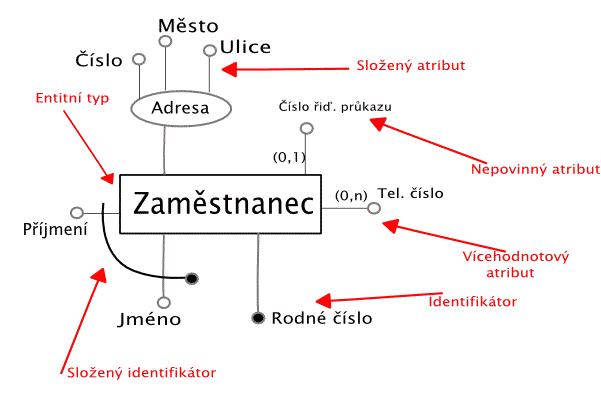
\includegraphics[width=14cm]{informatika/databazy/obrazky/er1.png}

(Entitn� typ se v�emo�n�mi druhy atribut�)
\end{center}
\end{obecne}

\begin{obecne}{Vztahov� typ}
\emph{Vztahov� typ} (v diagramu zna�en� koso�tvercem) popisuje vztahy mezi jednotliv�mi entitami -- s t�mi entitami, se kter�mi je v n�jak�m vztahu, je spojen �arou. Vztah m��e m�t danou i \emph{kardinalitu} (kolik entit z ka�d� strany do vztahu vstupuje), kter� m��e b�t typu $1:1$, $1:n$, $m:n$ a je zna�en� vedle ��ry spojuj�c� vztahov� typ s entitou. Entity ve vztahu mohou m�t nav�c \emph{povinn� �i nepovinn� �lenstv�} (vstupovat do n�j v�dy nebo jen n�kdy).

Vztahy mohou b�t bu� bin�rn� nebo obecn� $n$-�rn�, ale v�ce ne� tern�rn� vztahy se v�t�inou neobjevuj�. Vztahy mohou b�t i rekurzivn�, tj. do vztah� vstupuj� entity stejn�ho typu. Instance vztahov�ho typu je jednozna�n� ur�ena identifik�tory instanc� entit ve vztahu. N�kter� entitn� typy mohou b�t spoluidentifikov�ny (nebo p��mo identifikov�ny) vztahem -- pak se naz�vaj� \emph{slab� entitn� typy}.

\begin{center}
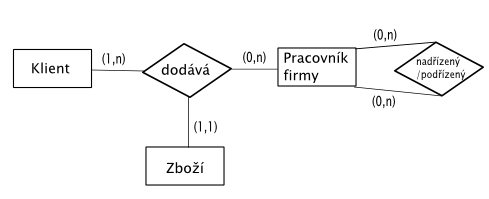
\includegraphics[width=12cm]{informatika/databazy/obrazky/er2.png}

(Vztahov� typy)
\end{center}
Obr�zek ukazuje tern�rn� vztah s r�zn�mi kardinalitami -- klientovi n�kdo dod�v� zbo�� jednou a� $n$-kr�t, pracovn�k dod�v� nula a� $n$-kr�t zbo�� (tj. jde o nepovinn� �lenstv� ve vztahu, m��ou existovat pracovn�ci, kte�� nic nedod�vaj�) a zbo�� je v�dy n�komu dod�v�no pr�v� jednou. Na zam�stnanc�ch je z�rove� uk�z�n rekurzivn� bin�rn� vztah.


\begin{center}
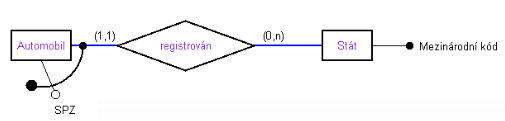
\includegraphics[width=10cm]{informatika/databazy/obrazky/er3.png}

(Slab� entitn� typ. Zdroj: slidy Dr. T. Skopala k Datab�zov�m syst�m�m)
\end{center}
Tento obr�zek ukazuje, jak vypad� slab� entitn� typ -- automobil je identifikov�n svoj� SPZ a z�rove� st�tem, ve kter�m je registrov�n.
\end{obecne}


\begin{obecne}{ISA hierarchie}
ISA hierarchie je roz���en� ER diagram� o \uv{d�di�nost} entit -- tj. rozd�len� entitn�ch typ� na subtypy (a p�id�n� dal��ch vztah� nebo atribut� pro subtypy). V ISA hierarchii se povoluje pouze jednon�sobn� d�di�nost, nav�c potomci n�jak�ho entitn�ho typu mus� b�t jednozna�n� identifikov�ni p�edkem (tj. v�echny entity v hierarchii sd�l� identifik�tor).

\begin{center}
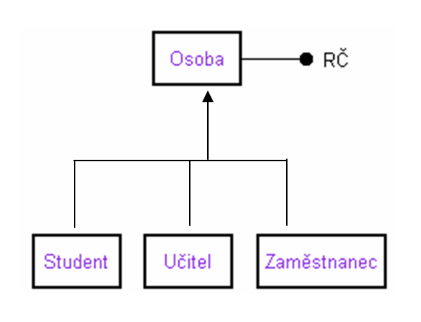
\includegraphics[width=6cm]{informatika/databazy/obrazky/er4.png}

(ISA hierarchie. Zdroj: slidy Dr. T. Skopala k Datab�zov�m syst�m�m)
\end{center}
\end{obecne}

\begin{obecne}{�pravy ER diagram�}
V ER diagramu je mo�n� prov�d�t v�cem�n� \uv{ekvivalentn�} �pravy (v�sledn� diagram reprezentuje stejn� koncept datab�ze), nap�. pro odstran�n� vztah� s kardinalitou $m:n$ (p�evod na dva vztahy kardinalitami $1:n$ a \emph{pr�nikov� entitn� typ}, kter� je vztahy ur�en�, tak�e je slab�). Dal��m d�vodem �prav m��e b�t zbaven� se ISA hierarchie. To se d� prov�st v�ce zp�soby, p�i�em� ��dn� z nich nefunguje �pln� obecn�:
\begin{pitemize}
    \item agregace atribut� a vztah� potomka do p�edka a �prava kardinalit (p�evod na nepovinn� atributy a nepovinn� �lenstv� ve vztahu)
    \item odstran�n� p�edka a duplikace v�ech jeho atribut� a vztah� v potomc�ch
    \item nahrazen� ISA vztahu klasick�m vztahem (z potomk� vzniknou slab� entitn� typy)
\end{pitemize}
Jin� �prava je odstran�n� v�cehodnotov�ho atributu -- p�evede se na vztah s kardinalitou $1:n$ a slab� entitn� typ.
\end{obecne}

\begin{obecne}{Korektn� ER sch�ma}
V \emph{korektn�m} ER sch�matu v�echny entity a vztahy spl�uj�:
\begin{pitemize}
    \item ��dn� entitn� typ nem� v�ce ne� jednoho ISA p�edka.
    \item ISA vztahy netvo�� orientovan� cyklus.
    \item Identifika�n� vztahy netvo�� orientovan� cyklus.
    \item Potomek v ISA hierarchii nen� identifika�n� z�visl� na ��dn�m entitn�m typu (je ji� identifikov�n p�edkem).
    \item Jm�na entitn�ch a vztahov�ch typ� jsou jednozna�n�.
\end{pitemize}
\end{obecne}


TODO: Co je ksakru \uv{ metody n�vrh� IS}?

\subsection{SQL}

Zdroje: slidy z p�edn�ek Datab�zov� syst�my a Datab�zov� aplikace Dr. T. Skopala a Dr. M. Kopeck�ho.

\subsubsection*{Standardy SQL}

SQL (\emph{Structured query language}) je standardn� jazyk pro p��stup k rela�n�m datab�z�m (a dotazov�n� nad nimi). Je z�rove� jazykem pro definici dat (definition data language), vytv��en� a modifikace sch�mat (tabulek), manipulaci s daty (data manipulation language), vkl�d�n�, aktualizace, maz�n� dat, ��zen� transakc�, definici integritn�ch omezen� aj. Jeho syntaxe odr�� snahu o co nejp�irozen�j�� formulace po�adavk� -- je podobn� anglick�m \uv{v�t�m}.

SQL je standard podle norem ANSI/ISO a existuje v n�kolika (zp�tn� kompatibiln�ch) verz�ch (ozna�ovan�ch podle roku uveden�):
\begin{description}
    \item[SQL 86] -- prvn� \uv{n�st�el}, pr�nik implementac� SQL firmy IBM
    \item[SQL 89] -� mal� revize motivovan� komer�n� sf�rou, mnoho detail� ponech�no implementaci
    \item[SQL 92] �- mnohem siln�j�� a obs�hlej�� jazyk. Zahrnuje u�
    \begin{pitemize}
	\item modifikace sch�mat, tabulky s metadaty, 
	\item vn�j�� spojen�, mno�inov� operace
	\item kask�dov� maz�n�/aktualizace podle ciz�ch kl���, transakce
	\item kurzory, v�jimky
    \end{pitemize}
    Standard existuje ve �ty�ech verz�ch: Entry, Transitional, Intermediate a Full.
    \item[SQL 1999] -� p�in�� mnoho nov�ch vlastnost�, nap�. 
    \begin{pitemize}	
	\item objektov�-rela�n� roz���en�
	\item nov� datov� typy -- reference, pole, full-text
	\item podpora pro extern� datov� soubory, multim�dia
	\item triggery, role, programovac� jazyk, regul�rn� v�razy, rekurzivn� dotazy ...
    \end{pitemize}
    \item[SQL 2003] -� dal�� roz���en�, nap�. XML management
\end{description}

Komer�n� syst�my implementuj� SQL podle r�zn�ch norem, n�kdy jenom SQL-92 Entry, dnes nej�ast�ji SQL-99, ale nikdy �pln� striktn�. N�kter� v�ci chyb� a naopak maj� v�echny spoustu nep�enositeln�ch roz���en� -- nap�. specifick� roz���en� pro procedur�ln�, transak�n� a dal�� funkcionalitu (T-SQL (Microsoft SQL Server), PL-SQL (Oracle) ). S nov�mi verzemi se kompatibilita zlep�uje, �asto je mo�n� pou��vat oboj� syntax. P�enos aplikace za b�hu na jinou platformu je ale st�le velice n�ro�n� -- a to t�m n�ro�n�j��, ��m v�c v�c� mimo SQL-92 Entry obsahuje. Pro otestov�n�, zda je �patn� syntax SQL, nebo zda jen dan� datab�zov� platforma nepodporuje n�kter� prvek, slou�� SQL valid�tory (kter� testuj� SQL podle norem).


\subsubsection*{Dotazy v SQL}

Hlavn�m n�strojem dotaz� v SQL je p��kaz \texttt{SELECT}. Sd�l� prvky rela�n�ho kalkulu i rela�n� algebry -- obsahuje pr�ci se sloupci, kvantifik�tory a agrega�n� funkce z rela�n�ho kalkulu a dal�� operace -- projekce, selekce, spojen�, mno�inov� operace -- z rela�n� algebry. Na rozd�l od striktn� formulace rela�n�ho modelu datab�ze povoluje duplik�tn� ��dky a NULLov� hodnoty atribut�.

Net��d�n� dotaz v SQL sest�v� z:
\begin{pitemize}
    \item p��kazu(�) \texttt{SELECT} (hlavn� logika dotazov�n�), to obsahuje v�dy
    \item m��e obsahovat i mno�inov� operace nad v�sledky p��kaz� \texttt{SELECT} -- \texttt{UNION}, \texttt{INTERSECTION} ...
\end{pitemize}
V�sledky nemaj� definovan� uspo��d�n� (resp. jejich po�ad� je ur�eno implementac� vyhodnocen� dotazu).

P��kaz \texttt{SELECT} vypad� n�sledovn� (tato verze u� zahrnuje i t��d�n� v�sledk�):
\begin{verbatim}
SELECT [DISTINCT]
 v�raz1 [[AS] c_alias1] [, ...]
FROM
 zdroj1 [[AS] t_alias1] [, ...]
[WHERE podm�nka_�]
[GROUP BY v�raz_g1 [, �]
[HAVING podm�nka_s]]
[ORDER BY v�raz_o1 [, �] ASC/DESC]
\end{verbatim}
Kde
\begin{pitemize}
    \item v�razy mohou b�t sloupce, sloupce s agrega�n�mi funkcemi, v�sledky dal��ch funkc� ...

\noindent \texttt{ v�raz = <n�zev sloupce>, <konstanta>, \\
 (DISTINCT) COUNT(~<n�zev sloupce>~),\\
{}[DISTINCT] [~SUM~|~AVG~](~<v�raz>~),\\
{}[~MIN~|~MAX~](~<v�raz>~)}\\
a nav�c lze pou��t oper�tory $+,-,*,/$.

    \item zdroje jsou tabulky nebo vno�en� selecty
    \item v�razy i zdroje b�t p�ejmenov�ny pomoc� \texttt{AS}, nap�. pro odkazov�n� uvnit� dotazu nebo jm�na na v�stupu (od SQL-92)
    \item podm�nka je logick� podm�nka (spojovan� logick�mi spojkami \texttt{AND, OR}) na hodnoty dat ve zdroj�ch:

\texttt{podm�nka = <v�raz> BETWEEN <x> AND <y>, <v�raz> LIKE "\%\_ ... ",\\
<v�raz> IS [NOT] NULL,\\
<v�raz> > = <> <= < > [<v�raz>/ ALL / ANY <dotaz>],\\
<v�raz> NOT IN [<seznam hodnot> / <dotaz>], EXIST ( <dotaz> )}

    \item \texttt{GROUP BY} znamen� agregaci podle unik�tn�ch hodnot jmenovan�ch sloupc� (v ostatn�ch sloupc�ch vznikaj� mno�iny hodnot, kter� se spolu s on�mi unik�tn�m� vyskytuj� na stejn�ch ��dk�ch
    \item \texttt{HAVING} ozna�uje podm�nku na agregaci
    \item \texttt{ORDER BY} definuje, podle hodnot ve kter�ch sloupc�ch nebo podle kter�ch jin�ch v�raz� nad nimi proveden�ch se m� v�sledek set��dit (\texttt{ASC} po�aduje vzestupn� set��d�n�, \texttt{DESC} sestupn�).
\end{pitemize}

SQL nem� p��kaz na omezen� rozsahu na n�kter� ��dky (jako nap�. \uv{pot�ebuji jen 50.-100. ��dek v�pisu}), a to lze �e�it bu� slo�it� standardn� (po��t�n� kolik hodnot je men��ch ne� vybran�, nav�c n�ro�n� na hardware) nebo pomoc� n�kter�ho nep�enositeln�ho roz���en�.

\medskip\noindent
Po�ad� vyhodnocov�n� jednoho p��kazu \texttt{SELECT} (nebereme v �vahu optimalizace):
\begin{penumerate}
    \item Nejprve se zkombinuj� data ze v�ech zdroj� (tabulek, pohled�, poddotaz�). Pokud jsou odd�leny ��rkami, provede se kart�zsk� sou�in (to sam� co \texttt{CROSS JOIN}), v SQL-92 a vy���m i slo�it�j�� spojen� -- \texttt{JOIN ON} (vnit�n� spojen� podle podm�nky), \texttt{NATURAL JOIN} (\uv{p�irozen�} spojen� podle stejn�ch hodnot stejn� pojmenovan�ch sloupc�), \texttt{OUTER JOIN} (\uv{vn�j��} spojen�, do kter�ho jsou zahrnuty i z�znamy, pro kter� v jednom ze zdroj� nen� nalezeno nic, co by odpov�dalo podm�nce, dopln�nn� NULLov�mi hodnotami) atd.
    \item Vy�ad� se vznikl� ��dky, kter� nevyhovuj� podm�nce (\texttt{WHERE})
    \item Zbyl� ��dky se seskup� do skupin se stejn�mi hodnotami uveden�ch v�raz� (\texttt{GROUP BY}), ka�d� skupina obsahuje atomick� sloupce s hodnotami uveden�ch v�raz� a mno�inov� sloupce se skupinami ostatn�ch hodnot sloupc�.
    \item Vy�ad� se skupiny, nevyhovuj�c� podm�nce (\texttt{HAVING})
    \item V�sledky se set��d� podle po�adavk�
    \item Vygeneruje se v�stup s po�adovan�mi hodnotami
    \item V p��pad� \texttt{DISTINCT} se vy�ad� duplicitn� ��dky
\end{penumerate}


\begin{e}{Pozn�mka}{0}{0}
\begin{pitemize}
    \item Klauzule \texttt{GROUP BY} set��d� p�ed vytvo�en�m skupin v�echny ��dky dle v�raz� v klauzuli. Proto by se m�l seskupovat co nejmen�� mo�n� po�et ��dek. Pokud je mo�n� ��dky odfiltrovat pomoc� WHERE, je v�sledek efektivn�j��, ne� n�sledn� odstra�ov�n� cel�ch skupin.
    \item  Klauzule \texttt{DISTINCT} t��d� v�sledn� z�znamy (p�ed operac� ORDER BY), aby na�la duplicitn� z�znamy. Pokud to jde, je vhodn� se bez n� obej�t.
    \item Klauzule \texttt{ORDER BY} by m�la b�t pou�ita jen v nutn�ch p��padech. Nen� p��li� vhodn� ji pou��vat v definic�ch pohled�, nad kter�mi se d�le d�laj� dal�� dotazy.
\end{pitemize}
\end{e}


\subsubsection*{Definice a manipulace s daty, ostatn� p��kazy}

Standard SQL podporuje n�kolik druh� datov�ch typ�:
\begin{pitemize}
    \item textov� v n�rodn� a glob�ln� (UTF) znakov� sad� (n�kolika druh� -- prom�nn� a pevn� d�lky): \texttt{CHARACTER(n)}, \texttt{NCHAR(n)},
    \texttt{CHAR VARYING(n)}
    \item ��seln� typy -- \texttt{ NUMERIC(p[,s]), INTEGER, INT, SMALLINT,\\  FLOAT(presnost), REAL, DOUBLE PRECISION}
    \item datumov� typy -- \texttt{DATE, TIME, TIMESTAMP, TIMESTAMP(presnost\_sekund) WITH TIMEZONE}
\end{pitemize}
Datab�zov� servery ne v�dy podporuj� v�echny uveden� typy. Nemus� je podporovat nativn�, n�kdy si pouze \uv{p�elo��} n�zev typu na podobn� nativn� podporovan� typ.

\medskip
\begin{obecne}{P��kaz \texttt{CREATE TABLE}}
Tento p��kaz slou�� k vytvo�en� nov� tabulky. Je nutn� definovat jej� n�zev, atributy a jejich dom�ny (datov� typy); d�le je mo�n� definovat integritn� omezen� (kl��e, ciz� kl��e, odkazy, podm�nky). P��kaz vypad� n�sledovn�:
\begin{center}
\texttt{CREATE TABLE <n�zev> <def. sloupce/i.o. tabulky, ...> }
\end{center}
A uvnit� potom
\begin{verbatim}
def. sloupce = <n�zev> <dat.typ> 
    [DEFAULT NULL|<hodnota>] [<i.o.sloupce>] 
dat.typ = [VARCHAR(n) | BIT(n) | INTEGER | FLOAT | DECIMAL ...] 
i.o.sloupce = [CONSTRAINT <jm�no>] [NOT NULL / UNIQUE / PRIMARY KEY], 
    REFERERENCES <tabulka>(<sloupec>) <akce>, CHECK <podm�nka> 
akce = [ON UPDATE / ON DELETE] 
    [CASCADE / SET NULL / SET DEFAULT / NO ACTION(hl�en� chyby) ] 
i.o.tabulky = UNIQUE, PRIMARY KEY <sloupec, ... >, 
    FOREIGN KEY <sloupec, ... >, 
    REFERENCES <tabulka>(<sloupec, ... >), 
    CHECK( <podm�nka> )
\end{verbatim}
\end{obecne}

\medskip
\begin{obecne}{P��kazy pro manipulaci se sch�matem}
\begin{pitemize}
    \item �prava tabulky:
\begin{verbatim}
ALTER TABLE <n�zev> ADD {COLUMN} <def.sloupce>, ADD <i.o.tabulky>, 
    ALTER COLUMN <sloupec> [ SET / DROP ], DROP COLUMN <sloupec>, 
    DROP CONSTRAINT <jm�no i.o.> 
\end{verbatim}
    \item Smaz�n� tabulky (nen� to sam� jako vymaz�n� v�ech dat z tabulky!):
\begin{verbatim}
DROP TABLE <tabulka> 
\end{verbatim}
    \item Vytvo�en� \uv{pohledu} -- navenek se chov� jako tabulka, ale vnit�n� se p�i ka�d�m dotazu provede vno�en� dotaz (kter� definic� pohledu zapisuji):
\begin{verbatim}
CREATE VIEW <n�zev "tabulky"> ( <sloupec, ... > ) 
    AS <dotaz> {WITH [ LOCAL / CASCADED ] CHECK OPTION }
\end{verbatim}
    N�kter� datab�zov� platformy umo��uj� do takto vytvo�en�ch pohled� i zapisovat.
\end{pitemize}
\end{obecne}

\medskip
\begin{obecne}{P��kazy pro manipulaci s daty}
\begin{pitemize}
    \item Vlo�en� nov�ch dat do tabulky
\begin{verbatim}
INSERT INTO <tabulka> ( <sloupec, ... > ) 
    [VALUES ( <v�raz, ... > ) / (<dotaz>) ] 
\end{verbatim}
    \item �prava dat (na ��dc�ch kter� vyhovuj� podm�nce se nastav� zadan� hodnoty vybran�m sloupc�m):
\begin{verbatim}
UPDATE <tabulka> SET 
    ( <sloupec> = [ NULL / <v�raz> / <dotaz> ] , ... ) 
    WHERE (<podm�nka>) 
\end{verbatim}
    \item Smaz�n� ��dk� vyhovuj�c�ch podm�nce z tabulky:
\begin{verbatim}
DELETE FROM <tabulka> ( WHERE <podm�nka> ) 
\end{verbatim}
\end{pitemize}
\end{obecne}

TODO: doplnit ?

\subsection{Indexy, triggery, ulo�en� procedury, u�ivatel�}

TODO: po��dn� definice indexu

\begin{obecne}{Index}
Index je obvykle definov�n v�b�rem tabulky a jej�ho konkr�tn�ho sloupce (nebo sloupc�), nad kter�mi si design�r datab�ze p�eje dotazov�n� urychlit; d�le pak technick�m ur�en�m typu. Chov�n� a zp�soby ulo�en� index� se mohou v�znamn� li�it podle pou�it� datab�zov� technologie.
V�jimku mohou tvo�it nap��klad full-textov� indexy, kter� jsou v n�kter�ch p��padech (nerela�n� datab�ze typu Lotus Notes) definov�ny nad celou datab�z�, nikoliv nad konkr�tn� tabulkou. 
\end{obecne}

\begin{obecne}{Pou�it� indexu}
Na prvn� pohled by se mohlo zd�t, �e ��m v�c index�, t�m lep�� chov�n� datab�ze a �e po vytvo�en� index� pro v�echny sloupce v�ech tabulk�ch dos�hneme maxim�ln�ho zrychlen�. Tento p��stup nar�� bohu�el na dva z�sadn� probl�my: 
\begin{penumerate}
    \item Ka�d� index zab�r� v pam�ti vyhrazen� pro datab�zi nezanedbateln� mno�stv� m�sta (vzhledem k pam�ti vyhrazen� pro tabulku). P�i existenci mnoha index� se m��e st�t, �e pam� zabran� pro jejich chod je skoro stejn� velk�, jako pam� zabran� jej�mi daty - zvl�t� u rozs�hl�ch tabulek (typu faktov�ch tabulek v datov�m skladu) m��e n�co takov�ho b�t nep�ijateln�. 
    \item Ka�d� index zpomaluje operace, kter� m�n� obsah indexovan�ch sloupc� (nap��klad SQL p��kazy UPDATE, INSERT). To je d�no t�m, �e datab�ze se v p��pad� takov� operace nad indexovan�m sloupcem mus� postarat nejen o zm�ny v datech tabulky, ale i o zm�ny v datech indexu. 
\end{penumerate}
\end{obecne}

\begin{obecne}{Typy index�}
Indexy mohou m�t sv�j typ, kter� bl�e ur�uje, jak�m zp�sobem m� b�t p�istupov�n� k dat�m tabulky optimalizov�no. Ozna�en� se r�zn�, ale nej�ast�ji je to:
\begin{pitemize}
    \item PRIMARY - Tento typ se v ka�d� tabulce m��e vyskytovat nejv��e jednou. Definuje sloupec tabulky, kter� svou hodnotou jednozna�n� identifikuje z�znam. Ve v�t�in� p��pad� se dodr�uje konvence takov� sloupec nazvat ID a jeho datov� typ stanovit jako cel� ��slo (nen�-li pot�eba jinak). Datab�zov� server by m�l b�t schopen nedopustit, aby byla do sloupce, k n�mu� se tento typ indexu vztahuje, byla vlo�ena hodnota, kter� ji� v tabulce existuje (v�t�inou takov� pokus kon�� chybovou hl�kou). 
    \item UNIQUE - Tento typ je podobn� PRIMARY co do jednozna�nosti z�znamu v tabulce (jak nazna�uje i jeho n�zev) a dopadu, kter� to na pr�ci s datab�z� m�; ale m��e se vyskytovat u v�ce sloupc� tabulky. Podle ��elu, ke kter�mu m� tabulka slou�it, se ob�as definuj� indexy slo�en� z v�ce sloupc� - potom op�t nelze vlo�it z�znam, kter� by ji� v t�to kombinaci n�kde v tabulce existoval. 
    \item INDEX - Definic� indexu tohoto typu je v tabulce zaji�t�na optimalizace vyhled�v�n� podle sloupce, ke kter�mu se dan� index v�e. V�t�inou si datab�zov� server vytvo�� a nad�le udr�uje vnit�n� seznam odkaz� na ��dky tabulky, se�azen� podle hodnot sloupce, k n�mu� se v�e. Udr�ov�n� takto se�azen� posloupnosti urychluje vyhled�v�n� (je mo�no pou��t n�kter� interpola�n� numerick� metody), �azen� i jin� z�sahy do tabulky, kter� jsou omezeny podm�nkou na doty�n� z�znamy. 
    \item FULL-TEXT - Vytvo�en�m tohoto indexu se datab�zov� server bude sna�it optimalizovat full-textov� vyhled�v�n� v dan�m sloupci u dan� tabulky.
\end{pitemize}
\end{obecne}

\begin{obecne}{Triggery}
  Datab�zov� trigger je programov� k�d, kter� je automaticky vykon�n jako
  reakce na n�jakou ud�lost v ur�it� datab�zov� tabulce. Triggery mohou omezit
  p��stup k ur�it�m dat�m, prov�d�t logov�n�, nebo kontrolovat zm�ny dat.

  Rozli�ujeme dv� hlavn� t��dy trigger� a to \emph{��dkov� trigger} a
  \emph{dotazov� (statement) trigger}. ��dkov� trigger m��eme definovat pro
  ka�d� ��dek tabulky, zat�mco dotazov� trigger se vykon� pouze jednou pro
  konkr�tn� datab�zov� dotaz. Ka�d� t��da trigger� m��e b�t n�kolika typ�. Jsou
  \emph{before triggers} a \emph{after triggers}, co� zna�� kdy m� b�t trigger
  vykon�n. Tak� se m��eme setkat s \emph{instead of triggers}, kter� je potom
  vykon�n \emph{m�sto} dotazu kter�m byl spu�t�n. 

  Jak� ud�losti mohou trigger spustit se pochopiteln� li�� datab�zov� syst�m od
  syst�mu, ale existuj� t�i typick� ud�losti, kter� to mohou b�t:
  \begin{penumerate}
    \item INSERT~-- nov� z�znam je vlo�en do datab�ze,
    \item UPDATE~-- z�znam je m�n�n,
    \item DELETE~-- z�znam je maz�n.
  \end{penumerate}
  Krom� t�chto typick�ch ud�lost� m��e datab�zov� syst�m umo��ovat nastavovat
  triggery tak� na maz�n�, �i vytv��en� cel�ch tabulek, �i dokonce p�ihl�en�
  nebo odhl�en� u�ivatele.

  Hlavn� vlastnosti a efekty datab�zov�ch trigger� jsou:
  \begin{pitemize}
    \item nep�ij�maj� ��dn� parametry nebo argumenty,
    \item nemohou volat operace pro ��zen� transakc� COMMIT a ROLLBACK,
    \item maj� p��stup k dat�m, kter� budou m�n�ny, je tedy mo�n� vykon�vat akce
    na z�klad� nich,
    \item nemohou vracet z�znamy,
    \item obt�n� se lad�,
    \item mnoho trigger� nebo slo�it� triggery mohou pr�ci s datab�z� velice
    zpomalit a nav�c znep�ehlednit.
  \end{pitemize}
\end{obecne}

\begin{obecne}{K �emu triggery pou��vat?}
  Triggery se v datab�z�ch pou��vaj� z n�kolika d�vod�, kter� mohou souviset s
  konzistenc� dat, jejich �dr�bou, nebo mohou b�t zp�sob, kter�m datab�ze
  komunikuje s okol�m. Pod�vejme se na n�kter� typick� sch�mata:
  \begin{pitemize}
    \item \textbf{Konzistence dat}~-- Trigger m��e prov�st v�po�et a na z�klad�
    toho povolit nebo nepovolit zm�nu dat v datab�zi. Nap��klad trigger m��e zak�zat
    smaz�n� z�kazn�ka z datab�ze v p��pad�, kdy m� u n�s n�jak� dluh a podobn�.  
    \item \textbf{Logov�n�}~-- Trigger m��e evidovat kdo, kdy a jak m�nil data.
    Lze tak dohledat pracovn�ka, kter� zadal �patn� �daje nebo zjistit, v kolik
    hodin do�lo k v�erej�� uz�v�rce.
    \item \textbf{Verzov�n� dat}~-- D�ky trigger�m lze snadno naprogramovat
    aplikaci tak, aby jedna tabulka udr�ovala historii zm�n tabulky jin�. To lze
    s �sp�chem pou��t t�eba jako bezpe�nostn� mechanismus. 
    \item \textbf{Zas�l�n� zpr�v}~-- Trigger m��e spustit n�jak� extern�
    program nebo proces. Nap��klad m��e trigger autorovi poslat e-mail,
    pokud byl k jeho �l�nku p�id�n p��sp�vek.
  \end{pitemize}
\end{obecne}

\begin{obecne}{Ulo�en� procedury}
  Ulo�en� procedura (anglicky stored procedure) je datab�zov� objekt, kter�
  neobsahuje data, ale ��st programu, kter� se nad daty v datab�zi m� vykon�vat.

  Ulo�en� procedura je p�edev��m procedura. Jedn� se o ��st programu, kter� je
  (nebo by aspo� m�l b�t) jasn� funk�n� odd�len� od sv�ho okol�, m� interface
  (seznam parametr�) pro komunikaci s jin�mi moduly programu. M��e m�t vlastn�
  lok�ln� prom�nn� neviditeln� pro ostatn� ��sti programu. 

  Ulo�en� procedura je ulo�en� (rozum�j: ulo�en� v datab�zi). To znamen�, �e se k
  n� lze chovat stejn� jako ke ka�d�mu jin�mu objektu datab�ze (indexu, pohledu,
  triggeru apod.). Lze j� zalo�it, upravovat a smazat pomoc� p��kaz� dotazovac�ho
  jazyka datab�ze (v p��pad� rela�n� datab�ze obvykle pomoc� p��kaz� DDL SQL). 

  Pro psan� ulo�en�ch procedur je obvykle pou��v�n specifick� jazyk konkr�tn�
  datab�ze, kter� je roz���en�m jej�ho dotazovac�ho jazyka (hezk�m p��kladem je
  datab�ze Oracle s procedur�ln�m jazykem PL/SQL, kter� je roz���en�m klasick�ho
  dotazovac�ho jazyka SQL).
\end{obecne}

\begin{obecne}{Pro� ukl�dat procedury?}
  \begin{pitemize}
      \item \textbf{Jednotn� rozhran�}~-- Pou�it� ulo�en�ch procedur vych�z� z
      faktu, �e v�t�ina operac� nad daty v datab�zi prob�h� stejn� bez ohledu na
      to, kdo operaci prov�d�. P��klad: Pokud je t�eba ulo�it do tabulky
      z�kazn�k� nov�ho z�kazn�ka, tak se to z pohledu datab�ze d�je stejn� pro
      z�kazn�ka internetov�ho obchodu, pro z�kazn�ka, kter�ho zad�v� pracovnice
      telefonick�ho centra p�es formul�� programu napsan�ho nap��klad v C++ ,
      nebo pro z�kazn�ky, kte�� jsou vkl�d�ni automaticky na z�klad� textov�ho
      reportu, kter� p�ijde ka�d� den z \uv{kamenn�ch} prodejn�ch m�st a je
      zpracov�v�n pomoc� programu napsan�ho v PowerBuilderu. Je tedy celkem
      dobr� d�vod, aby existovala ulo�en� procedura \uv{Zapi� nov�ho z�kazn�ka},
      kterou by mohly volat v�echny t�i v��e uveden� aplikace - alternativou bez
      ulo�en� procedury by bylo, �e bych podobnou proceduru musel napsat ve
      t�ech verz�ch - jednou v C++, jednou v Power Builderu a jednou v r�mci
      programu pro internetov� obchod (t�eba ASP nebo PHP). 
      \item \textbf{Skryt� datov�ch operac�}~-- Druhou v�hodou pou�it� ulo�en�ch
      procedur je, �e se nemus�m (v programu na \uv{klientsk�} stran�) zab�vat
      t�m, jak jsou data ulo�ena v konkr�tn�ch tabulk�ch. V na�em p��pad� je mi
      jedno, jak si datab�ze uvnit� pamatuje z�kazn�ky - prost� zad�m jako
      parametr procedury jm�no, p��jmen�, ��slo kreditky a co si z�kazn�k koupil
      - a datab�ze (resp. jej� ulo�en� procedura) si to n�jak p�ebere. Ulo�en�
      procedury se v p��pad� datab�zov�ch aplikac� staly z�kladn�m kamenem pro
      realizaci architektury klient/server, kdy je na jedn� stran� (klientsk�
      ��st) realizov�na v b�n�m procedur�ln�m programovac�m jazyku komunikace s
      u�ivatelem (formul��e nebo t�eba webov� str�nky) a na druh� stran�
      (serverov� ��st) je pomoc� ulo�en�ch procedur realizov�na spr�va dat v
      rela�n� datab�zi. Ob� ��sti (klientsk� a serverov�) mezi sebou komunikuj�
      p�es co nejjednodu��� rozhran� - vol�n�m ulo�en�ch procedur. 
  \end{pitemize}
\end{obecne}

TODO: u�ivatel�

\subsection{V�cevrstevn� architektury}

TODO: p�ed�lat, tohle je jen copy \& paste z Wiki a slajd� VUT Brno


\begin{obecne}{Multitier architecture}
Multi-tier architecture (often referred to as n-tier architecture) is a client-server architecture, originally designed by Jonathon Bolster of Hematites Corp, in which an application is executed by more than one distinct software agent. For example, an application that uses middleware to service data requests between a user and a database employs multi-tier architecture. The most widespread use of "multi-tier architecture" refers to three-tier architecture
\end{obecne}


\begin{obecne}{Z�klad kooperativn�ho zpracov�n�}
Faktory ovliv�uj�c� architekturu:
\begin{pitemize}
\item po�adavky na interoperabilitu zdroj� 
\item r�st velikosti zdroj� 
\item r�st po�tu klient� 
\end{pitemize}
Typy slu�eb v datab�zov� technologii:
\begin{pitemize}
\item prezenta�n� slu�by: p��jem vstupu, zobrazov�n� v�sledk� 
\item prezenta�n� logika: ��zen� interakce (hierarchie menu, obrazovek)
\item logika aplikace: operace realizuj�c� algoritmus aplikace
\item logika dat: podpora operac� s daty (integritn� omezen�, ...)
\item datov� slu�by: akce s datab�z� (definice a manipulace, transak�n� zpracov�n�, ...) 
\item slu�by ovl�d�n� soubor�: vlastn� V/V operace
\end{pitemize}
\end{obecne}

\begin{obecne}{Varianty architektury klient-server}
\begin{pitemize}
    \item \textbf{Klient-server se vzd�len�mi daty} \\
Na serveru jsou jen datov� slu�by a ovl�d�n� soubor�, zbytek zaji��uj� klienti. Probl�mem jsou velk� n�roky na p�enosovu kapacitu od klienta k serveru a HW zat�en� klientsk�ch stanic
    \item \textbf{Klient-server se vzd�lenou prezentac�} \\
Na klientsk� stanici jsou jen prezenta�n� slu�by a prezenta�n� logika, zbytek je na serveru. Nev�hodou je pr�v� z�t� na HW serveru.
    \item \textbf{Klient-server s rozd�lenou logikou} \\
��st logiky aplikac� i logiky dat je na serveru a ��st zpracov�v� klient. Jde o vyv�en� �e�en�, kter� m� ale hor�� roz���itelnost.
    \item \textbf{T��vrstv� architektura} \\
Zahrnuje dva servery -- aplika�n� a datab�zov�, spojen� rychlou linkou. Z hlediska z�t�e a roz���itelnosti nejv�hodn�j��.
\end{pitemize}
\end{obecne}

\begin{obecne}{P��nos architektury klient/server a t��vrstv� architektury}
\begin{pitemize}
 \item pru�n�j�� rozd�len� pr�ce \item lze pou��t horizont�ln�(v�ce server�) i vertik�ln�(v�konn�j�� server) �k�lov�n� \item aplikace mohou b�et na levn�j��ch za��zen�ch \item na klientsk�ch stanic�ch lze pou��vat obl�ben� prezenta�n� software \item standardizovan� p��stup umo��uje zp��stupnit dal�� zdroje \item centralizace dat podporuje ��inn�j�� ochranu \item u t��vrstv� architektury centralizace �dr�by aplikace, mo�nost vyu�it� sd�len�ch objekt� (business objects) n�kolika aplikacemi
\end{pitemize}
\end{obecne}

\begin{obecne}{Podpora pro rozd�len� z�t�e v architektu�e klient/server}
\begin{pitemize}
 \item deklarativn� integritn� omezen� \item datab�zov� triggery \item ulo�en� podprogramy
\end{pitemize}
\end{obecne}


\begin{obecne}{Three-tier architecture}
'Three-tier' is a client-server architecture in which the user interface, functional process logic ("business rules"), data storage and data access are developed and maintained as independent modules, most often on separate platforms. The term "three-tier" or "three-layer", as well as the concept of multitier architectures, seems to have originated within Rational Software.

The three-tier model is considered to be a software architecture and a software design pattern.

Apart from the usual advantages of modular software with well defined interfaces, the three-tier architecture is intended to allow any of the three tiers to be upgraded or replaced independently as requirements or technology change. For example, a change of operating system from Microsoft Windows to Unix would only affect the user interface code.

Typically, the user interface runs on a desktop PC or workstation and uses a standard graphical user interface, functional process logic may consist of one or more separate modules running on a workstation or application server, and an RDBMS on a database server or mainframe contains the data storage logic. The middle tier may be multi-tiered itself (in which case the overall architecture is called an "n-tier architecture").

The 3-Tier architecture has the following 3-tiers:
\begin{pitemize}
    \item Presentation Tier
    \item Application Tier/Logic Tier/Business Logic Tier
    \item Data Tier
\end{pitemize}
\end{obecne}


\begin{obecne}{Web Development usage}

In the Web development field, three-tier is often used to refer to Websites, commonly Electronic commerce websites, which are built using three tiers:
\begin{pitemize}
    \item A front end Web server serving static content
    \item A middle dynamic content processing and generation level Application server, for example Java EE platform.
    \item A back end Database, comprising both data sets and the Database management system or RDBMS software that manages and provides access to the data.
\end{pitemize}
\end{obecne}

\begin{obecne}{Other Considerations}

To further confuse issues, the particular data transfer method between the 3 tiers must also be considered. The data exchange may be file-based, client-server, event-based, etc. Protocols involved may include one or more of SNMP, CORBA, Java RMI, Sockets, UDP, or other proprietary combinations/permutations of the above types and others. Typically a single "middle-ware" implementation of a single protocol is chosen as the "standard" within a given system, such as J2EE (which is Java specific) or CORBA (which is language/OS neutral.) The importance of the decision of which protocol is chosen affects such issues as the ability to include legacy applications/libraries, performance, maintainability, etc. When choosing a "middle-ware protocol" (not to be confused with the "middle-of-the-three-tiers") engineers should not be swayed by "public opinion" about a protocol's modern-ness, but should consider the technical benefits and suitability to solve a problem. (for example CGI is very old and "out of date" but is still quite useful and powerful, so is shell scripting, and UDP for that matter)

Ideally the high-level system abstract design is based on business rules and not on the front-end/back-end technologies. The tiers should be populated with functionality in such a way as to minimize dependencies, and isolate functionalities in a coherent manner - knowing that everything is likely to change, and changes should be made in the fewest number of places, and be testable.
\end{obecne}

\subsection{Vazba datab�z� na internetov� technologie}

TODO: v�echno


\subsection{Organizace dat na vn�j�� pam�ti, B-stromy a jejich varianty}


\subsubsection*{Vn�j�� pam�}

\begin{e}{Definice}{0}{Vn�j�� pam�}
\emph{Vn�j�� pam�} je �lo�i�t� dat (pam�ov� m�dium), u kter�ho je rychlost na��t�n� dat zpravidla n�zk� a p��stup k nim ne �pln� p��m� (z�le�� na uspo��d�n� dat na m�diu), ne-li pouze sekven�n� (oproti vnit�n� pam�ti s rychl�m n�hodn�m p��stupem a men�� kapacitou). P��kladem vn�j�� pam�ti je pevn� disk nebo magnetick� p�ska.

\emph{Magnetick� p�sky} poskytuj� vysokou kapacitu, ale n�zkou rychlost a pouze sekven�n� p��stup. Pro jejich kapacitu je d�le�it� hustota z�znamu, pot�ebuj� meziblokov� mezery pro vyrovn�n� nep�esnosti p�et��en� p�sky.

\emph{Pevn� disky} umo��uj� p��m� p��stup, ale jeho rychlost nen� v�dy stejn�. Ovliv�uje ji fyzick� vzd�lenost dat -- pevn� disk m� n�kolik \emph{v�lc�}, na nich� jsou ulo�eny jednotliv� datov� \emph{stopy}. K v�lc�m p��slu�� \emph{�tec� hlavy} (je jich stejn� jako v�lc�, ale pohybuj� se v�echny sou�asn�, tak�e m��e v 1 okam�iku ��st jen jedna). Disky jsou v�t�inou rozd�leny na \emph{sektory} -- nejmen�� jednotku dat, kterou je mo�n� na��st nebo ulo�it (zpravidla jednotky KB). Pro rychlost p��stupu k dat�m jsou d�le�it� tyto veli�iny (v�robcem disk� jsou zpravidla ud�v�ny pr�m�rn� hodnoty):
\begin{pitemize}
    \item \emph{seek} ($s$) -- p�esun na jinou stopu, dnes zpravidla kolem 4-8~ms
    \item \emph{(average) rotational delay} ($r$) -- oto�en� v�lc� -- 1 p�lot��ka, pro nej�ast�j�� 7200rpm disk je to cca 4~ms
    \item \emph{block transfer time} ($btt$) -- doba p�enesen� 1 bloku po sb�rnici, na ATA/100 disku se 4~KB bloky teoreticky 0.04~ms
\end{pitemize}
Pokud jsou data um�st�na na disku za sebou sekven�n�, rychlost jejich na�ten� je mnohem vy��� ne� p�i n�hodn�m rozm�st�n�, proto�e nen� t�eba prov�d�t p�esuny mezi stopami a ot��en� v�lc� nav�c.
\end{e}

\begin{e}{P��klad}{0}{0}
\emph{Jak vypad� na�ten� 1~MB dat z pevn�ho disku?} P�edpokl�dejme, �e na 1 stopu se vejde 512~KB a 1 blok m� 4~KB. Jsou-li data um�st�na na disku sekven�n�, pot�ebuji pro na�ten� 1~MB dat naj�t prvn� blok a potom ��st dv� cel� stopy (2 ot��ky), tj. celkem $s+r+(2\cdot2r)$ (a p�enos po sb�rnici lze zanedbat, proto�e prob�h� z�rove� se �ten�m). Pokud jsou data na disku n�hodn� rozprost�ena, pot�ebuji celkem 256-kr�t naj�t blok a na��st ho: $256\cdot(s+r+btt)$, tak�e operace trv� a� 100-kr�t d�le.
\end{e}


\subsubsection*{Soubor}

\begin{e}{Definice}{0}{Z�znam, kl��}
\emph{(Logick�) z�znam} je jednotka dat (nap�. v datab�zi), m� \emph{atributy} (z nich� ka�d� m� jm�no a dom�nu -- povolenou mno�inu hodnot). Logick�mu z�znamu v reprezentaci na disku odpov�d� \emph{fyzick� z�znam} (n�jak� d�lky $R$ -- pevn� nebo prom�nn�), kter� nav�c m��e obsahovat je�t� dal�� data -- odd�lova�e, ukazatele, hlavi�ky. 

\emph{Kl��} je mno�ina atribut�, kter� jednozna�n� identifikuje z�znam; proti tomu \emph{vyhled�vac� kl��} je mno�ina atribut�, pro kterou lze nal�zt mno�inu odpov�daj�c�ch z�znam�. Vyhled�vac� kl��e jsou t�� druh�: hodnotov� (\uv{oby�ejn�} hodnoty n�kter�ch atribut�), ha�ovan� a relativn� (p��mo pozice v souboru).
\end{e}

\begin{e}{Definice}{0}{Soubor}
(Homogenn�) \emph{soubor} je multimno�ina z�znam�. Fyzicky na vn�j�� pam�ti je organizov�n do \emph{blok� (str�nek)} (velikosti $B$, typicky n�kolika KB) -- hl. jednotkou p�enosu dat mezi vnit�n� a vn�j�� pam�t�. Pom�r velikosti z�znamu k velikosti bloku ($B/R$) se naz�v� \emph{blokovac� faktor} ($\lfloor b\rfloor$). Z�znamy mohou b�t rozprost�eny i p�es n�kolik str�nek, nebo m��e b�t pouze jeden z�znam na 1 str�nku; ide�ln� (ale ne v�dy dosa�iteln�) je, pokud beze zbytku zapl�uj� str�nky. Na souboru jsou definov�ny operace se z�znamy: \emph{insert, delete, update} a \emph{fetch}.
\end{e}

\begin{e}{Definice}{0}{Dotaz}
\emph{Dotaz} je ka�d� funkce, kter� ka�d�mu sv�mu argumentu p�i�ad� odpov�daj�c� mno�inu z�znam� ze souboru (\uv{tot�ln� vy��sliteln� funkce definovan� na souboru}). Dotazy mohou b�t t�chto typ�:
\begin{pitemize}
    \item Na�ten� v�ech z�znam� ({\tt SELECT * FROM tabulka})
    \item Na �plnou shodu ({\tt SELECT * FROM tabulka WHERE sloupec1 = 'hodnota' AND sloupec2 = 'hodnota'} pro tabulku se 2 sloupci -- d�ny jsou v�echny atributy)
    \item Na ��ste�nou shodu\\({\tt SELECT * FROM tabulka WHERE sloupec1 = 'hodnota'} pro tabulku se 2 sloupci -- zadan� je jen ��st atribut�)
    \item Na intervalovou shodu (��ste�nou nebo �plnou) ({\tt SELECT * FROM tabulka WHERE sloupec1 > 'hodnota'})
\end{pitemize}
U soubor� se sleduje rychlost proveden� t�chto operac�.
\end{e}


\subsubsection*{Statick� metody organizace souboru}

\begin{e}{Definice}{0}{Sch�ma organizace souboru}
\emph{Sch�ma organizace souboru} je popis logick� pam�ov� struktury, do n� lze zobrazit logick� soubor, spolu s algoritmy operac� nad touto strukturou. Ta je obvykle tvo�ena z logick�ch str�nek (blok� pevn� d�lky) a m��e popisovat v�ce prov�zan�ch log. soubor�, z nich� \emph{prim�rn� soubor} je ten, kter� obsahuje u�ivatelsk� data. Operace definovan� nad sch�matem org. souboru jsou krom� operac� nad soubory je�t� \emph{build, reorganization, open} a \emph{close}.

Proti n�mu stoj� \emph{fyzick� sch�ma souboru} -- struktura nad fyzick�mi soubory, nejbl�e hardwaru je \emph{implementa�n� sch�ma souboru}.

Zaji�t�n� \emph{Vyv�enosti struktury} znamen� zaji�t�n� omezen� cesty p�i vyhled�v�n� n�jak�m v�razem (zaru�en� asymptotick� slo�itosti), nav�c zaru�en� rovnom�rnosti zapln�n� struktury -- \emph{faktor napln�n� str�nek}. Sch�mata, kter� spl�uj� ob� podm�nky, se naz�vaj� \emph{dynamick�}, ostatn� jsou ozna�ov�na jako \emph{statick�}.
\end{e}

\begin{e}{Pozn�mka}{0}{�asov� odhady}
Pro sch�mata organizace soubor� se po��taj� �asov� odhady proveden� jednotliv�ch operac� -- jednodu���ch, jako je p��stup k z�znamu ($T_F$), \emph{rewrite} -- p�epis b�hem 1 ot��ky disku ($T_{RW}$), p��p. sekven�n� �ten�; d�le i slo�it�j��ch jako vyhled�n� z�znamu, p�id�n�, smaz�n� a �prava z�znamu, reorganizace struktury nebo na�ten� cel�ho souboru.
\end{e}

\begin{obecne}{Hromada (neuspo��dan� sekven�n� soubor)}
\emph{Hromada(heap)} je naprosto nejjednodu��� sch�ma organizace souboru, kdy jsou z�znamy v souboru jen n�hodn� se�azeny za sebou. �asov� slo�itost vyhled�v�n� je $O(n)$, pokud $n$ je po�et z�znam�. Jde o \emph{nehomogenn� soubor}, kde z�znamy obvykle nemaj� pevnou d�lku. 
\end{obecne}

\begin{obecne}{Uspo��dan� sekven�n� soubor}
V \emph{uspo��dan�m sekven�n�m souboru} jsou z�znamy �azeny podle kl��e. Aktualizovan� z�znamy se um�st� do zvl�tn�ho souboru a a� p�i dal�� operaci \uv{reorganization} jsou p�id�ny do prim�rn�ho. Slo�itost nalezen� z�znamu je tak� $O(n)$, ale pokud se hled� podle kl��e, podle kter�ho jsou z�znamy se�azeny, a nav�c je soubor na m�diu s p��m�m p��stupem, sn�� se na $O(\log n)$.
\end{obecne}

\begin{obecne}{Index-sekven�n� soubor}
Toto sch�ma uva�uje prim�rn� soubor jako sekven�n�, uspo��dan� podle prim�rn�ho kl��e. Nad n�m je pak vytvo�en (t�eba i v�ce�rov�ov�) \emph{index}. Ten sest�v� ze seznamu ��sel str�nek a minim�ln�ch hodnot kl��e jim odpov�daj�c�ch z�znam�. Pokud m� index v�c �rovn�, prov�d� se pro vy��� �rovn� to sam� na bloc�ch index� �rovn� o 1 ni���. Nejvy��� �rove� indexu se obvykle vejde do 1 bloku, tzv. \emph{master}. 

Po�et pot�ebn�ch �rovn� pro $n$ z�znam� se d� spo��tat jako $\lceil\log_p\frac{n}{\lfloor b\rfloor}\rceil$, kde $p=\lfloor\frac{B}{V+P}\rfloor$ p�i velikosti kl��e $V$ a pointeru na str�nku $P$. Probl�mem je p�id�v�n� nov�ch z�znam�, kdy se tyto �et�z� za sebe v tzv. \emph{oblasti p�ete�en�} (ka�d� z nich m� pointer na dal�� z�znam v oblasti p�ete�en�). Pro odd�len� nutnosti vkl�d�n� do oblasti p�ete�en� lze inici�ln� bloky plnit na m�n� ne� 100\%.
\end{obecne}


\begin{obecne}{Indexovan� soubor}
\emph{Indexovan� soubor} znamen� prim�rn� soubor plus indexy pro r�zn� vyhled�vac� kl��e. Neindexuj� se u� str�nky, ale p��mo z�znamy, a proto prim�rn� soubor nemus� b�t nutn� set��d�n�. Index m��e b�t podobn� jako u index-sekven�n�ho souboru, pro z�znamy se stejn�m kl��em je ale vhodn�, aby byly na v�ech �rovn�ch indexu krom� posledn� slou�en�. P�i aktualizaci se nepou��v� oblast p�ete�en�, m�n� se pouze index.

Existuje i n�kolik dal��ch variant index�. Pro zmen�en� n�ro�nosti dotaz� na kombinovanou ��ste�nou shodu se pou��v� \emph{kombinovan� index} pro v�ce atribut�, u n�ho� je ale nutn� p�edem zjistit na kter� kombinace atribut� budou �asto pokl�d�ny dotazy, a pro takov� kombinace tento index teprve vytvo�it. \emph{Clusterovan� index} zaru�uje, �e z�znamy s podobnou hodnotou indexovan�ho atributu jsou bl�zko sebe v prim�rn�m souboru -- nap�. pokud je prim�rn� soubor podle tohoto atributu set��d�ny. Tento index lze pou��t jen pro 1 atribut. 

\emph{Bitov� mapy} se daj� pou��t jako index pro atributy s malou dom�nou (mno�inou mo�n�ch hodnot) -- pro ka�dou hodnotu t�to dom�ny se vyrob� vektor bit� stejn� d�lky, jako je po�et z�znamu v prim�rn�m souboru, kde jedni�ka na $i$-t� pozici indikuje, �e $i$-t� z�znam m� pr�v� tuto hodnotu atributu. To umo��uje jednoduch� prov�d�n� booleovsk�ch dotaz� na tento atribut. Vektory bit� nav�c lze komprimovat, tak�e nezab�raj� tolik m�sta.
\end{obecne}

\begin{obecne}{Soubor s p��m�m p��stupem}
V tomto sch�matu jsou z�znamy v prim�rn�m souboru (\uv{adresov�m prostoru} velikosti $M$) rozpt�leny pomoc� \emph{hashovac� funkce}. �asto se pou��v� funkce $h=k\mod M'$, kde $M'$ je nejbli��� prvo��slo men�� ne� velikost adresov�ho prostoru. Hashovac� funkc� se ur�uje bu� jenom ��slo str�nky, nebo i relativn� pozice v n�. P�i hashov�n� vznikaj� kolize, kter� se daj� �e�it \emph{otev�en�m adresov�n�m} (�et�zen�m kolizn�ch z�znam� za sebe), \emph{rehashov�n�m} (dal�� funkc�) nebo pou�it�m \emph{oblasti p�ete�en�}. Snaha je v�t�inou um�stit kolizn� z�znamy do stejn� str�nky. 

Pokud je hashovac� funkce prost�, jedn� se o \emph{perfektn� hashov�n�}. Toho ale v praxi vlastn� nelze dos�hnout, tak�e se tento v�raz pou��v� i pro ozna�en� stavu, kdy je pro nalezen� z�znamu pot�eba nejv�� $O(1)$ p��stup� k m�diu. O�ek�van� d�lka �et�zce koliz� p�i po�tu $N$ z�znam� v prostoru velikosti $M$ je $1/(1-\frac{N}{M})$.
\end{obecne}

\subsubsection*{T��d�n� na vn�j�� pam�ti}

\begin{e}{Algoritmus}{0}{T��d�n� sl�v�n�m (Mergesort)}
Tento algoritmus se pou��v� pro t��d�n� dat, kter� se nevejdou do vnit�n� pam�ti. D� se pou��t i p�i sekven�n�m p��stupu k datov�m soubor�m. Nejjednodu��� verze bez buffer� vypad� takto:
\begin{pitemize}
    \item inicializace: na za��tku ka�d�ho kroku data rozd�l� do 2 soubor�
    \item na�te 2 z�znamy, ka�d� z jednoho souboru a porovn� je
    \item ve spr�vn�m po�ad� je zap�e do v�stupn�ho souboru, ze vstupn�ho souboru si na�te dal�� dva
    \item v prvn�m kroku z�sk�m uspo��dan� posloupnosti d�lky 2; v dal��ch kroc�ch v�dy porovn�m na�ten� prvky, zap�u men�� z nich a ze souboru odkud tento poch�zel si na�tu dal��, tak�e z�sk�m v�dy uspo��dan� posloupnosti dvojn�sobn� d�lky ne� v p�edchoz�m kroku
    \item po $\lceil\log n\rceil$ kroc�ch je soubor s $n$ z�znamy set��d�n�.
\end{pitemize}
Vylep�en� se dos�hne nap�. p��mo st��dav�m zapisov�n�m v�stupu do 2 soubor�, kdy se zbav�m nutnosti na za��tku ka�d�ho kroku data d�lit, nebo pou�it�m v�ce soubor� najednou. Je taky mo�n� vyu��t rostouc�ch posloupnost� prvk�, kter� se v souboru nach�zej� ji� p�ed zapo�et�m t��d�n�.
\end{e}

\begin{e}{Algoritmus}{0}{T��d�n� haldou}
Pro t��d�n� ve vnit�n� pam�ti se pou��v� algoritmus \emph{t��d�n� haldou (heapsort)}, kter� se d� zakomponovat do vylep�en� t��d�n� sl�v�n�m (viz n�e). Jeho z�kladem je datov� struktura \emph{halda} (konkr�tn� maxim�ln� halda, max-heap), reprezentovan� jako pole z�znam�, na kter�m je bin�rn� stromov� struktura: z�znam $k$ m� v�dy vy��� kl�� ne� jeho dva synov�, nach�zej�c� se na pozic�ch $2k+1$ a $2k+2$ p�i ��slov�n� od $0$ (pokud tato pozice nen� v�t�� ne� velikost haldy, v opa�n�m p��pad� z�znam nem� syny). Na pozici $0$ se tak nach�z� z�znam s nejvy���m kl��em. Postup t��d�n� je n�sledovn�:
\begin{pitemize}
    \item nejv�t�� prvek (z pozice $0$) se prohod� s t�m prvkem, jeho� ��slo pozice odpov�d� aktu�ln� velikosti haldy
    \item velikost haldy se zmen�� o 1
    \item dokud neplat� podm�nka, �e kl�� prvku z�skan�ho z konce haldy je v�t�� ne� oba kl��e jeho syn�, prohazuje se tento se synem s v�t��m kl��em (a tak posouv� v hald� d�l)
    \item toto se opakuje, dokud je velikost haldy v�t�� ne� 1, odzadu tak v poli vznik� set��d�n� posloupnost
\end{pitemize}
�asov� slo�itost algoritmu je $O(n\cdot\log n)$ pro pole z�znam� velikosti $n$.
\end{e}

\begin{e}{Algoritmus}{0}{$n$-cestn� t��d�n�}
Pokud m�m k dispozici ve vnit�n� pam�ti $n+1$ str�nek, mohu postupovat n�sledovn�:
\begin{pitemize}
    \item v 1. kroku na��st do pam�ti $n$ str�nek
    \item ty set��dit pomoc� heapsortu (nebo i quicksortu apod.) a z�skat tak del�� set��d�n� �seky (\emph{b�hy})
    \item sl�vat v�dy $n$ nejkrat��ch b�h� (pomoc� mergesortu) a vytv��et tak jeden b�h
    \item toto opakovat, dokud existuje v�ce ne� 1 b�h.
\end{pitemize}
�as. slo�itost pro $M$ str�nek v souboru je $O(2M\lceil\log_n M/n\rceil)$.
\end{e}

\begin{e}{Algoritmus}{0}{Dvojit� halda}
Del�� b�hy p�i sl�v�n� se daj� vytv��et pomoc� dvojit� haldy -- v pam�ti m�m dv� haldy z celkem $n$ prvk�, opakovan� z prvn� haldy odeb�r�m a zapisuji minim�ln� prvek do v�stupn�ho b�hu a na��t�m dal�� prvek, pokud ten je v�t�� ne� minimum haldy, vlo��m ho do prv� haldy, pokud je men��, vlo��m ho do druh� haldy, kter� vznik� od konce m�ho pole. A� se prvn� halda vy�erp�, pou�iji druhou a za�nu nov� b�h. Toto v nejhor��m p��pad� d�v� stejnou velikost b�h� jako oby�ejn� halda, pr�m�rn� je 2x lep��.
\end{e}


\subsubsection*{B-stromy}

\begin{e}{Definice}{0}{B-strom}
B-strom ��du $m$ je v��kov� vyv�en� strom, kter� m� n�sl. vlastnosti:
\begin{penumerate}
    \item Ko�en m� minim�ln� 2 syny, pokud nen� s�m listem.
    \item Ka�d� jin� uzel krom� list� m� nejm�n� $\lceil\frac{m}{2}\rceil$ a nejv�ce $m$ syn� a v�dy o 1 m�n� dat. z�znam� (listy maj� jen datov� z�znamy).
    \item Kl��e v�ech z�znam� v $i$-t�m podstromu uzlu $A$ jsou v�t�� ne� kl�� $i$-t�ho z�znamu uzlu $A$ a men�� nebo rovny kl��i $i+1$-t�ho z�znamu.
    \item v�echny \emph{v�tve} (cesty od ko�ene k listu) jsou stejn� dlouh�.
\end{penumerate}
Variantou jsou \emph{redundantn� B-stromy}, kdy v�echna data jsou um�st�na v listech, vnit�n� uzly obsahuj� pouze vyhled�vac� kl��e. Jin� mo�nost je pou�it� pouze kl��e a odkazu na cel� z�znam, m�sto vkl�d�n� kompletn�ch z�znam� do stromu.
\end{e}

\begin{e}{Algoritmus}{0}{Operace na B-strom�}
\emph{Vyhled�v�n�} v B-stromech podle kl��e se prov�d� jednoduch�m pr�chodem do hloubky.

\emph{Vkl�d�n�} prob�h� tak, �e se najde m�sto, kam z�znam vlo�it, pokud nen� uzel pln�, prost� se z�znam vlo��, jinak se uzel roz�t�p�, p�lka prvk� se d� vlevo, p�lka vpravo a prost�edn� se vlo�� (�mezi n�) do otce. Pokud v otci nen� m�sto, pokra�uje se stejn�m zp�sobem a� do ko�ene, kde se p��padn� vytvo�� nov� uzel a ud�l� se z n�j ko�en.

\emph{Odeb�r�n�} prvk� je opa�n� postup, v p��pad� podte�en� uzlu (z�stane v n�m m�n� ne� $\lceil\frac{m}{2}\rceil$ syn�) mus�m p�eb�rat data od sousedn�ch uzl� nebo sl�vat. V redundantn�ch B-stromech nen� nutn� p�i maz�n� odstra�ovat vyhled�vac� kl�� z vnit�n�ch uzl� -- prvek s touto hodnotou se ve strom� u� nebude nach�zet, ale vyhled�vat podle jeho kl��e je d�l mo�n�.
\par
Lep�� napln�nosti uzl� za cenu sn�en� rychlosti se d� dos�hnout pomoc� \emph{vyva�ov�n� str�nek} -- p�i p�ete�en� str�nky nejd��v kontroluji, jestli nejsou voln� sousedn�; pokud ano, p�erozd�l�m data a uprav�m kl��e. Podobn� je mo�n� postupovat p�i maz�n� (i pokud nen� t�eba sl�vat).
\par
Dal��m vylep�en�m je odlo�en� �t�pen� -- ke ka�d�mu listu nebo skupin� list� p��slu�� str�nka p�ete�en�, kam se vkl�daj� z�znamy, kter� se u� do dan�ho m�sta nevejdou. Nov� vkl�d�n� a �t�pen� je provedeno a� tehdy, jestli�e se str�nka p�ete�en� i v�echny p��slu�n� uzly napln�. Takto upraven� strom s v�ce ne� 1 �rovn� m� v�dy v�echny listy zapln�n� (za p�edpokladu nepou�it� maz�n�). P��slu��-li str�nky p�ete�en� skupin�m list�, mus�m je p�i maz�n� a p�id�v�n� list� takt� �t�pit a sl�vat.
\end{e}

\begin{e}{Definice}{0}{B+ stromy}
\emph{B+ stromy} jsou m�rn�m vylep�en�m B-strom� pro zrychlen� intervalov�ch dotaz�: v�echny uzly ve stejn� �rovni (a nebo jenom listy) jsou spojeny do spojov�ho seznamu (mo�n� je jednosm�rn� i obousm�rn� varianta).
\end{e}

\begin{e}{Definice}{0}{B* stromy}
\emph{B* stromy} (��du $m$) jsou �pravou B-strom� na z�klad� vyva�ov�n� str�nek. Druh� podm�nka B-strom� se uprav� tak, �e ka�d� uzel krom� ko�ene a list� m� minim�ln� $\lceil(2m-1)/3\rceil$ a max. $m$ syn� a odpov�daj�c� po�et dat. z�znam�. Listy maj� op�t jen stejn� rozmez� pro po�et dat. z�znam�. P�i vkl�d�n� prvk� se st�pen� odkl�d� op�t do t� doby, dokud nejsou pln� i sourozenci dan�ho listu; potom se �t�p� bu� 2 listy do 3, nebo 3 do 4 (bu� s pomoc� jednoho nebo dvou sousedn�ch sourozenc�). Odeb�r�n� podobn� zahrnuje sl�v�n� 3 uzl� do 2 (nebo 4 do 3). P�i ob�m lze ve slo�it�j�� variant� zapojit je�t� v�ce uzl�.
\end{e}

\begin{e}{Definice}{0}{Prefixov� stromy (Trie)}
Tento druh strom� slou�� k ulo�en� dat, kl��ovan�ch �et�zci. Jde o redundantn� stromy, data jsou ulo�ena a� v listech; vyhled�vac� kl��e jsou v�dy co nejkrat�� mo�n� prefixy �et�zc�, nutn� k odli�en� uzl�. Cel� hodnoty kl��� (a dal�� data) se nach�zej� a� v listech. P�i vkl�d�n� a �t�pen� str�nek se n�jakou heuristikou hled� nejkrat�� prefix, kter� by vznikl� str�nky odd�lil. Vylep�en� varianta neukl�d� u syn� p�edponu kl��e, kterou m� rodi� -- je to pam�ov� efektivn�j��, ale zvy�uje v�po�etn� n�roky.
\end{e}

\begin{e}{Definice}{0}{Stromy s prom�nnou d�lkou z�znamu}
Jde o modifikaci B-stromu, kter� umo��uje do n�j ulo�it z�znamy prom�nn� d�lky. Listy se ne�t�p� podle po�tu z�znam�, ale zhruba na poloviny podle velikosti dat. Druh� podm�nka B-strom� se uprav� n�sledovn�: celkov� d�lka z�znam� v jednom uzlu je minim�ln� $\lceil B/2\rceil$ a maxim�ln� $B$ (kde $B$ je n�jak� zvolen� hodnota, v�t�. velikost str�nky na disku). Existuje i varianta s podm�nkou \uv{$2/3$}, jako maj� B*-stromy.

Probl�mem t�to struktury je tendence del��ch z�znam� ke stoup�n� ke ko�eni, ��m� se sni�uje arita z�znam�. To se �e�� hled�n�m d�l�c�ho z�znamu s min. d�lkou tak, aby vznikl� uzly spl�ovaly podm�nky stromu (a je to docela n�ro�n�). Nav�c �t�pen� je slo�it�j�� -- 1 str�nka se m��e �t�pit na 3 (vlo��m-li hodn� dlouh� z�znam), m��e doj�t ke zmen�en� stromu p�i vlo�en� apod., b�n� se pou��v� obecn� algoritmus nahrazov�n�, jeho� speci�ln� p��pady jsou insert a delete.
\end{e}


\begin{e}{Definice}{0}{V�cerozm�rn� B-stromy}
Pou��vaj� se, je-li pot�eba efektivn� hledat z�znamy podle v�ce atribut�. Jde o propojenou mno�inu strom�. K jednotliv�m atribut�m p��slu�ej� prvky pole odkaz� na seznamy strom�, ve kter�ch se podle dan�ch atribut� d� hledat. Pro prvn� atribut je pot�eba jen 1 strom, v n�m je pro ka�d� kl�� odkaz na cel� strom 2. atributu (pro dal�� je to podobn�). Stromy stejn�ho atributu jsou ve spojov�m seznamu. Mohu hledat v�echny z�znamy, pro kter� zn�m hodnoty v�ech atribut�, nebo jenom jejich podmno�inu -- vy�aduje to proj�t v�ce strom�, ale nen� t�eba mno�inov�ch operac�.
\end{e}


\section{Programovací jazyky a překladače}
\begin{pozadavky}
\begin{pitemize}
\item Principy a základy implementace objektově orientovaných jazyků a jazyků s blokovou strukturou, běhová podpora vyšších programovacích jazyků
\item Oddělený překlad, sestavení, řízení překladu
\item Neprocedurální programování
\item Struktura překladače, lexikální, syntaktická analýza
\item Interpretované jazyky, virtuální stroje
\item Pojmy a principy objektového návrhu
\item Generické programování a knihovny
\item Návrhové vzory
\end{pitemize}
\end{pozadavky}
\subsection{Principy a z�klady implementace objektov� orientovan�ch jazyk� a jazyk� s blokovou strukturou, b�hov� podpora vy���ch programovac�ch jazyk�}

\textsl{Z�kladn� v�domosti:} \textit{ T��da, D�di�nost, Polymorfismus, Obalen�, Virtu�ln� funkce. B�hov� podpora vy���ch programovac�ch jazyk�: Statick� podpora a dynamick� podpora, Rozd�len� pam�ti, Stav pam�ti p�ed spu�t�n�m, Konstruktory, destruktory glob�ln�ch prom�nn�ch, Volac� konvence.}

TODO: jde hlavn� o copy \& paste z Wikipedie, tak�e by to cht�lo omezit zbyte�n� kecy a p�elo�it to, co je anglicky. Ot�zkou je taky, jestli sem �vodn� �l�nek v�bec pat��. Ja mysl�m �e jo, ale jist� si nejsem.

\subsubsection*{Strukturovan� programov�n�}

Po��ta�ov� program je n�jak�m zp�sobem zaznamenan� postup po��ta�ov�ch operac�, kter� speci�ln�m zp�sobem popisuje praktickou realizaci zadan� �lohy (tedy algoritmus v�po�tu). Program z \emph{procedur�ln�ho} �hlu pohledu je vlastn� p�esn� specifikace v�ech krok�, kter� mus� po��ta� vykonat, aby do�el k c�li, a jejich po�ad�. Pro ur�ov�n� po�ad� krok� se pou��vaj� z�kladn� operace \emph{��zen� toku} -- skoky, podm�nky, cykly apod.

Jedn�m z d�le�it�ch koncept� procedur�ln�ho programov�n� je \emph{strukturovan� programov�n�} -- jeho idea je zalo�ena na rod�len� programu na \emph{procedury} (rutiny, podrutiny, metody, funkce), kter� samy obsahuj� v��et v�po�etn�ch krok� k vykon�n�, mohou b�t ale spou�t�ny opakovan� a z libovoln�ho m�sta v programu. Jejich v�hodou je mnohem n�zorn�j�� pohled na strukturu programu a snaz�� udr�ov�n� k�du, ne� v p��pad� pou�it� jen nejjednodu���ho ��zen� toku (tedy hlavn� skok�, kter� by se ve strukturovan�m programov�n� spr�vn� pou��vat nem�ly).

\medskip
Historically, several different structuring techniques or methodologies have been developed for writing structured programs. The most common are:
\begin{pitemize}
    \item \emph{Dijkstra's structured programming}, where the logic of a program is a structure composed of similar sub-structures in a limited number of ways. This reduces understanding a program to understanding each structure on its own, and in relation to that containing it, a useful separation of concerns.
    \item \emph{A view derived from Dijkstra's} which also advocates splitting programs into sub-sections with a single point of entry, but is strongly opposed to the concept of a single point of exit.
    \item \emph{Data Structured Programming}, which is based on aligning data structures with program structures. This approach applied the fundamental structures proposed by Dijkstra, but as constructs that used the high-level structure of a program to be modeled on the underlying data structures being processed.
\end{pitemize}
The two latter meanings for the term "structured programming" are more common. Years after Dijkstra (1969), object-oriented programming (OOP) was developed to handle very large or complex programs.

\medskip
\begin{definiceN}{Programovac� jazyk s blokovou strukturou}
A language is described as "block-structured" when it has a syntax for enclosing structures between bracketed keywords, such as an if-statement bracketed by \texttt{if..fi}, or a code section bracketed by \texttt{BEGIN..END}.

However, a language is described as "comb-structured" when it has a syntax for enclosing structures within an ordered series of keywords. A "comb-structured" language has multiple structure keywords to define separate sections within a block, analogous to the multiple teeth or prongs in a comb separating sections of the comb. For example, in Ada, a block is a 4-pronged comb with keywords DECLARE, BEGIN, EXCEPTION, END, and the if-statement in Ada is a 4-pronged comb with keywords IF, THEN, ELSE, END IF. Jako jazyk s \uv{h�ebenovou} strukturou by se dalo tedy br�t t�eba i PL/SQL.
\end{definiceN}

\begin{poznamka}
It is possible to do structured programming in any programming language, though it is preferable to use something like a procedural programming language. Since about 1970 when structured programming began to gain popularity as a technique, most new procedural programming languages have included features to encourage structured programming (and sometimes have left out features that would make unstructured programming easy). Some of the better known structured programming languages are Pascal, C, PL/I, and Ada.
\end{poznamka}

\begin{obecne}{V�ta o strukturovan�m programu???}
\emph{The structured program theorem} is a result in programming language theory. It states that every computable function can be implemented in a programming language that combines subprograms in only three specific ways. These three control structures are
\begin{pitemize}
    \item Executing one subprogram, and then another subprogram (\emph{sequence})
    \item Executing one of two subprograms according to the value of a boolean variable (\emph{selection})
    \item Executing a subprogram until a boolean variable is true (\emph{iteration})
\end{pitemize}

This observation did not originate with the structured programming movement; these structures are sufficient to describe the instruction cycle of a central processing unit, as well as the operation of a Turing machine. Therefore a processor is always executing a "structured program" in this sense, even if the instructions it reads from memory are not part of a structured program.
\end{obecne}


\subsubsection*{Datov� a~��d�c� struktury vy���ch programovac�ch jazyk� a~jejich implementace}

\begin{obecne}{��zen� toku}
In computer science control flow (or alternatively, flow of control) refers to the order in which the individual statements, instructions or function calls of an imperative or functional program are executed or evaluated. Within an imperative programming language, a control flow statement is an instruction that when executed can cause a change in the subsequent control flow to differ from the natural sequential order in which the instructions are listed. For non-strict functional languages, functions and language constructs exist to achieve the same ends, but they are not necessarily called control flow statements.

The kinds of control flow statements available differ by language, but can be roughly categorized by their effect:
\begin{pitemize}
    \item continuation at a different statement (jump),
    \item executing a set of statements only if some condition is met (choice -- if-then-else)
    \item executing a set of statements zero or more times, until some condition is met (loop), s~podm�nkou na za��tku, na konci, uprost�ed, nekone�n�, s~dan�m po�tem opakov�n�
    \item executing a set of distant statements, after which the flow of control may possibly return (subroutines, coroutines, and continuations),
    \item stopping the program, preventing any further execution (halt).
\end{pitemize}
Interrupts and signals are low-level mechanisms that can alter the flow of control in a way similar to a subroutine, but are usually in response to some external stimulus or event rather than a control flow statement in the language.
\end{obecne}

\begin{obecne}{V�jimky}
V�jimky jsou speci�ln�m p��kazem ��zen� toku, vyskytuj�c�m se v n�kter�ch vy���ch programovac�ch jazyc�ch. Z�kladn� my�lenkou je, �e program m��e na n�jak�m m�st� vyhodit v�jimku (p��kaz \texttt{throw}), co� zp�sob�, �e prov�d�n� programu se zastav� a bu� pokra�uje tam, kde je v�jimka \uv{o�et�ena} (tzv. \texttt{catch} blok), nebo pokud takov� m�sto nen� nalezeno, program skon�� s chybou. B�hem hled�n� m�sta o�et�en� je datov� hodnota v�jimky ulo�ena stranou a pak m��e b�t pou�ita.

P�i hled�n� m�sta o�et�en� v�jimky (\texttt{try}-bloku, n�sledovan�ho catch-blokem se spr�vn�m datov�m typem v�jimky) se postupuje zp�t po z�sobn�ku vol�n� funkc�, tato technika se naz�v� \uv{stack unwinding} (odv�jen� z�sobn�ku). V n�kter�ch jazyc�ch (Java) lze definovat i akci, kter� se provede v ka�d�m p��pad�, i pokud nastane v�jimka, je�t� p�ed odv�jen�m z�sobn�ku -- \texttt{finally} blok.
\end{obecne}

\begin{obecne}{Volac� konvence}
P�i vol�n� procedur a funkc� je nejd�le�it�j�� z�sobn�k. Ukl�d� se na n�j
\begin{pitemize}
    \item kam se vr�tit po vol�n�
    \item argumenty funkce (v p�ekladem definovan�m po�ad� -- nutn� m�t ve v�ech modulech stejn�; v�t�inou se li�� v z�vislosti na programovac�m jazyku)
    \item n�vratov� hodnota funkce
    \item ukazatel na s�manticky nad�azenou funkci (Pascal)
\end{pitemize}
Dohromady v�em t�mto dat�m se n�kdy ��k� \uv{aktiva�n� z�znam} procedury. Po skon�en� funkce je nutn� z�sobn�k op�t uklidit (vymazat zbyte�n� ulo�en� data, v�t�inou jen z�st�v� n�vratov� hodnota) a kter� ��st programu to d�l� (volan� nebo volaj�c� procedura), z�vis� op�t na p�eklada�i a konvenci jazyka.

\medskip\noindent
Volac� konvence dvou nejtypi�t�j��ch jazyk�:
\begin{pitemize}
\item \emph{Pascal} \\ ukl�z� volan� funkce, argumenty se ukl�daj� na z�sobn�k zleva doprava (nejlevej�� nejd��v, tj. nejhloub�ji)
\item \emph{C} \\ ukl�z� funkce volaj�c�, argumenty se ukl�daj� zprava doleva (tj. nejlev�j�� je na vrcholu z�sobn�ku. Je to kv�li funkc�m s prom�nn�m po�tem parametr�. Volan� funkce mus� podle prvn�ho argumentu poznat, jak� je skute�n� po�et argument�. Kdyby byl prvn� argument n�kde hluboko v~z�sobn�ku, tak v� prd.)
\end{pitemize}
\end{obecne}


\subsubsection*{Organizace pam�ti}

Pam� procesu (spu�t�n�ho programu) lze rozd�lit do n�kolika ��st�:
\begin{pitemize}
\item \emph{k�d programu (k�dov� segment)} \\
vytvo�en p�i p�ekladu, sou��st spustiteln�ho souboru, nem�nn� a m� pevnou d�lku; obvykle b�v� chr�n�n proti z�pisu
\item \emph{statick� data (datov� segment)} \\
data programu, jejich� velikost je zn�ma ji� p�i p�ekladu a jejich� pozice se b�hem programu nem�n� (je p�ipraven kompil�torem a jeho form�t je takt� zadr�tovan� ve spustiteln�m souboru, u inicializovan�ch statick�ch dat je tam cel� ulo�en�); v jazyce C jde o glob�ln� prom�nn� a lok�ln� data deklarovan� jako \texttt{static}, konstanty
\item \emph{halda (heap segment)} \\
vytv��en startovac�m modulem (C Runtime library), ukl�daj� se sem dynamicky vznikaj�c� objekty (\texttt{malloc, new}) -- neinicializovan� data, i seznam voln�ho m�sta
\item \emph{voln� pam�} \\
postupn� j� zapl�uje z jedn� strany z�sobn�k a z druh� halda
\item \emph{z�sobn�k (stack segment)} \\
informace o vol�n� procedur (\uv{aktiva�n� z�znamy}) --- n�vratov� adresy, parametry a n�vratov� hodnoty (nejsou-li p�ed�v�ny v registrech), n�kter� jazyky (Pascal, C) pou��vaj� i pro �schovu lok�ln�ch dat. Typicky roste z�sobn�k proti hald� (od \uv{konce} pam�ti k ni���m adres�m).
\end{pitemize}


\begin{poznamkaN}{Vno�en� funkce}
V Pascalu mohou b�t funkce definovan� uvnit� jin� funkce. Ta vnit�n� pot�ebuje p�istupovat k~prom�nn�m t� vn�j��. Prom�nn� jsou sice na z�sobn�ku, ale pouh� odkaz na volaj�c� funkci nesta��, proto�e se vno�en� funkce m��e volat rekurzivn�. Proto je na z�sobn�ku ukazatel na funkci s�manticky nad�azenou.
\end{poznamkaN}

\begin{obecne}{Alokace m�sta pro r�zn� typy prom�nn�ch}
\begin{pitemize}
    \item Dynamicky alokovan� prom�nn� (p�es pointer) se alokuj� na hald�. Opakovanou alokac� a~dealokac� pam�ov�ch blok� r�zn� velikosti vznikaj� v~hald� \uv{d�ry} (st��dav� �seky voln�ho a naalokovan�ho m�sta). Existuje n�kolik strategi� pro vyhled�n� voln�ho bloku po�adovan� velikosti (first-fit, next-fit, buddy syst�m) a udr�en� informac� o voln�m m�st�, kter� jsou v�t�inou implementov�ny v knihovn�ch funkc�ch jazyka (C, Pascal).
    \item Lok�ln� prom�nn� se ukl�daj� na z�sobn�k, po skon�en� funkce, kter� p��slu��, jsou zase odstran�ny.
    \item Glob�ln� a~statick� se ukl�daj� do segmentu pro statick� data. Tady se d�ry tvo�it nebudou, proto�e tyhle prom�nn� vznikaj� na za��tku a~zanikaj� na konci programu (tak�e se form�t segmentu nem�n�).
\end{pitemize}
\end{obecne}



\subsubsection*{Objektov�-orientovan� programov�n�}

\begin{obecne}{��el objektov�ho porgramov�n�}
In the 1960s, language design was often based on textbook examples of programs, which were generally small (due to the size of a textbook); however, when programs become very large, the focus changes. In small programs, the most common statement is generally the assignment statement; however, in large programs (over 10,000 lines), the most common statement is typically the procedure-call to a subprogram. Ensuring parameters are correctly passed to the correct subprogram becomes a major issue.

Many small programs can be handled by coding a hierarchy of structures; however, in large programs, the organization is more a network of structures, and insistence on hierarchical structuring for data and procedures can produce cumbersome code with large amounts of "tramp data" to handle various options across the entire program.

Although structuring a program into a hierarchy might help to clarify some times of software, even for some special types of large programs, a small change, such as requesting a user-chosen new option (text font-color) could cause a massive ripple-effect with changing multiple subprograms to propagate the new data into the program's hierarchy. The object-oriented approach is allegedly more flexible, by separating a program into a network of subsystems, with each controlling their own data, algorithms, or devices across the entire program, but only accessible by first specifying named access to the subsystem object-class, not just by accidentally coding a similar global variable name. Rather than relying on a structured-programming hierarchy chart, object-oriented programming needs a call-reference index to trace which subsystems or classes are accessed from other locations.
\end{obecne}


\begin{definiceN}{Objektov� orientovan� programov�n�}
Na objektov�-orientovan� programov�n� se d� nahl�dnout jako na kolekci spolupracuj�c�ch objekt� -- v protikladu k tradi�n�mu pohledu, kdy se za program pova�uje sled instrukc� pro po��ta�. V OOP je ka�d� objekt schopn� p�ij�mat zpr�vy, zpracov�vat data a pos�lat zpr�vy jin�m objekt�m. Na ka�d� objekt se tak d� nahl�et jako na nez�visl� \uv{mal� stroj} s vlastn� rol� a zodpov�dnost�. Zjednodu�en� �e�eno jde o~dota�en� konceptu \emph{data + algoritmy = program}. Data tvo�� s k�dem, kter� je spravuje, jeden celek.
\end{definiceN}

\begin{obecne}{Hlavn� koncepty (a form�ln�j�� definice)}
Objektov� orientovan� programov�n� (zkracov�no na OOP, z anglick�ho Object-oriented programming) je metodika v�voje softwaru, zalo�en� na n�sleduj�c�ch my�lenk�ch, koncepci:
\begin{pitemize}
\item \emph{Objekty}: jednotliv� prvky modelovan� reality (jak data, tak souvisej�c� funk�nost) jsou v programu seskupeny do entit, naz�van�ch objekty. Objekty si pamatuj� sv�j stav a navenek poskytuj� operace (p��stupn� jako metody pro vol�n�).
\item \emph{Abstrakce}: program�tor, pota�mo program, kter� vytv���, m��e abstrahovat od n�kter�ch detail� pr�ce jednotliv�ch objekt�. Ka�d� objekt pracuje jako �ern� sk���ka, kter� dok�e prov�d�t ur�en� �innosti a komunikovat s okol�m, ani� by vy�adovala znalost zp�sobu, kter�m vnit�n� pracuje.
\item \emph{Zapouzd�en�}: zaru�uje, �e objekt nem��e p��mo p�istupovat k \uv{vnit�nostem} jin�ch objekt�, co� by mohlo v�st k nekonzistenci. Ka�d� objekt navenek zp��stup�uje rozhran�, pomoc� kter�ho (a nijak jinak) se s objektem pracuje.
\item \emph{Skl�d�n�}: Objekt m��e vyu��vat slu�eb jin�ch objekt� tak, �e je po��d� o proveden� operace.
\item \emph{D�di�nost}: objekty jsou organizov�ny stromov�m zp�sobem, kdy objekty n�jak�ho druhu mohou d�dit z jin�ho druhu objekt�, ��m� p�eb�raj� jejich schopnosti, ke kter�m pouze p�id�vaj� svoje vlastn� roz���en�. Tato my�lenka se obvykle implementuje pomoc� rozd�len� objekt� do t��d, p�i�em� ka�d� objekt je instanc� n�jak� t��dy. Ka�d� t��da pak m��e d�dit od jin� t��dy (v n�kter�ch programovac�ch jazyc�ch i z n�kolika jin�ch t��d). Umo��uje zach�zet s~mno�inou t��d, jako by byly v�echny reprezentov�ny t�m sam�m objektem. Nap��klad zn�m� hierarchie: grafick� objekt, bod, kru�nice. Nav�c je to prost�edek pro �sporu pr�ce p�i k�dov�n�.
\item \emph{Polymorfismus}: odkazovan� objekt se chov� podle toho, jak� je jeho skute�n� typ. Pokud n�kolik objekt� poskytuje stejn� rozhran�, pracuje se s nimi stejn�m zp�sobem, ale jejich konkr�tn� chov�n� se li��. V praxi se tato vlastnost projevuje nap�. tak, �e na m�sto, kde je o�ek�v�na instance n�jak� t��dy, m��eme dosadit i instanci libovoln� jej� podt��dy (t��dy, kter� p��mo �i nep��mo z t�to t��dy d�d�), kter� se m��e chovat jinak, ne� by se chovala instance rodi�ovsk� t��dy, ov�em v r�mci \uv{mantinel�}, dan�ch popisem rozhran�.
\end{pitemize}
\end{obecne}

\begin{obecne}{T��da}
\emph{T��da} definuje abstraktn� vlastnosti n�jak�ho objektu, v��tan� obs�hnut�ch dat (atributy, pole (fields) a vlastnosti (properties)) a v�c�, kter� m��e d�lat (spr�van�, metody a schopnosti (features)). Nap��klad t��da \emph{Dog} by obsahovala v�ci spolo�n� pro v�echny psy - nap�. atrib�ty rasa, barba srsti a schopnosti b�echat. % tady prosim ten jazyk neopravujte, to je tak hezky :)!
 

T��dy poskytuj� v objektovo-orientovan�m programu modularitu a strukturu. T��da by typicky m�la b�t rozpoznateln� i ne-program�torovi, kter� se ale v dan� dom�n� probl�m� orientuje -- tzn. �e charakteristiky t��dy by m�li \uv{d�vat v kontextu smysl}. Podobn� i k�d t��dy by m�l b�t relativn� \uv{self-contained}. Vlastnosti a met�dy t��d se spolu naz�vaj� i \emph{members}.
\end{obecne}

\begin{obecne}{Implementace objekt�}
Z hlediska jazyka nen� velk� rozd�l mezi slo�en�mi datov�mi typy a t��dami. Deklarace t��dy obsahuje, stejn� jako u slo�en�ho dat. typu, datov� polo�ky. Nav�c ale obsahuje i deklarace funkc� (metod), kter� s nimi pracuj�. N�kter� funkce mohou m�t speci�ln� vlastnosti -- statick�, virtu�ln�, konstruktory, destruktory. Nav�c v�t�ina jazyk� p�id�v� mo�nost ozna�en� kter�chkoliv polo�ek jako ve�ejn� nebo priv�tn�. T��dy mohou n�kdy (C++, Java) obsahovat i vno�en� datov� typy (v��ty, ... ) a dokonce vno�en� t��dy.

Za b�hu je jedna instance t��dy -- objekt reprezentov�na v pam�ti pomoc�:
\begin{pitemize}
    \item datov�ch polo�ek (stejn� jako slo�en� datov� typ),
    \item skryt�ch pomocn� polo�ky umo��uj�c�ch funkci virtu�ln�ch metod, v�jimek, RTTI a d�di�nosti (identifikace typu / jeho velikosti apod.)
\end{pitemize}

\emph{Implementace d�di�nosti v C++:} Je-li t��da B (p��m�m �i nep��m�m) potomkem t��dy A, pak pam�ov� reprezentace objektu typu B obsahuje ��st, kter� m� stejn� tvar jako pam�ov� reprezentace samostatn�ho objektu typu A. Z ka�d�ho ukazatele na typ B je mo�no odvodit ukazatel na ��st typu A -- tato konverze je implicitn�, tj. nen� t�eba ji explicitn� uv�d�t ve zdrojov�m k�du. Tato konverze m��e (obvykle pouze p�i n�sobn� d�di�nosti) vy�adovat jednoduch� v�po�et (p�i�ten� posunut�).

Z ukazatele na typ A je mo�no odvodit ukazatel na typ B, jen pokud konkr�tn� objekt, do kter�ho ukazuje ukazatel na typ A, je typu B (nebo jeho potomka). Zodpov�dnost za ov��en� skute�n�ho typu objektu m� program�tor a tuto konverzi je t�eba explicitn� vynutit p�etypov�n�m. M��e to znamenat ode�ten� posunut� v pam�ti.
\end{obecne}

\begin{obecne}{Virtu�ln� funkce}
In object-oriented programming (OOP), a virtual function or virtual method is a function whose behavior, by virtue of being declared "virtual," is determined by the definition of a function with the same signature furthest in the inheritance lineage of the instantiated object on which it is called. This concept is a very important part of the polymorphism portion of object-oriented programming (OOP).

The concept of the virtual function solves the following problem:

In OOP when a derived class inherits from a base class, an object of the derived class may be referred to (or cast) as either being the base class type or the derived class type. If there are base class functions overridden by the derived class, a problem then arises when a derived object has been cast as the base class type. When a derived object is referred to as being of the base's type, the desired function call behavior is ambiguous.

The distinction between virtual and not virtual is provided to solve this issue. If the function in question is designated "virtual" then the derived class's function would be called (if it exists). If it is not virtual, the base class's function would be called.

\emph{Pozdn� vazba (late binding; virtual call):} Je-li metoda n�jak� t��dy virtu�ln� �i �ist� virtu�ln�, pak v�echny metody se stejn�m jm�nem, po�tem a typy parametr� deklarovan� v potomc�ch t��dy jsou pova�ov�ny za r�zn� implementace t�e funkce. Kter� implementace se vybere, tedy kter� t�lo bude zavol�no, se rozhoduje a� za b�hu programu podle skute�n�ho typu cel�ho objektu. Pou�ije se t�lo z posledn�ho potomka, kter� definuje tuto funkci a je sou��st� cel�ho objektu. Pozdn� vazba m� smysl pouze u vyvol�n� na objektu ur�en�m odkazem.

Pozdn� vazba je implementa�n� umo�n�n� skryt�m pointerem na \emph{tabulku virtu�ln�ch funkc�} uvnit� ka�d�ho objektu. Existuje pro ka�dou t��du jedna. P�i d�di�nosti z�st�v� v cel�m objektu odkaz jeden, ale (i pro \uv{nejvnit�n�j��} b�zovou t��du) odkazuje na tabulku odvozen� t��dy. V tabulce mus� b�t proto pointery na funkce, deklarovan� u� u b�zov� t��dy, um�st�ny na za��tku (aby bylo mo�n� volat funkce b�zov� t��dy mezi sebou bez zm�ny k�du).
\end{obecne}



\subsection{Oddělený překlad, sestavení, řízení překladu}

\subsubsection*{Struktura programu}

Program se skládá z \emph{modulů}:
\begin{pitemize}
	\item Překládány samostatně kompilátorem 
	\item Spojovány linkerem
\end{pitemize}
Modul z pohledu programátora
\begin{pitemize}
	\item Soubor s příponou .cpp (.c)
\end{pitemize}
Hlavičkové soubory
\begin{pitemize}
	\item Soubory s příponou .h
	\item Deklarují (a někdy i definují) identifikátory používané ve více modulech
	\item Vkládány do modulů direktivou include
	\begin{pitemize}
		\item Direktivu zpracovává preprocesor čistě textově
		\item Preprocesor je integrován v kompilátoru jako první fáze překladu
	\end{pitemize}
\end{pitemize}
Modul z pohledu kompilátoru
\begin{pitemize}
	\item Samostatná jednotka překladu
	\item Výsledek práce preprocesoru
\end{pitemize}

\subsubsection*{Oddělený překlad}

\par\begin{center}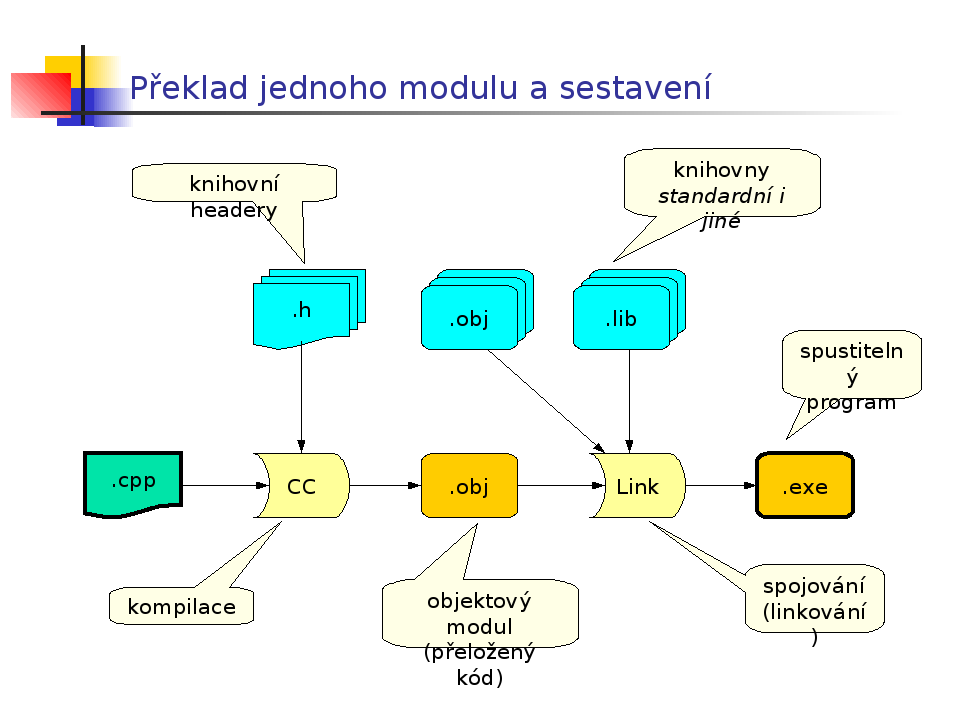
\includegraphics[width=10cm]{informatika/programovanie/obrazky/oddelenypreklad01.png}
\end{center}
\par\begin{center}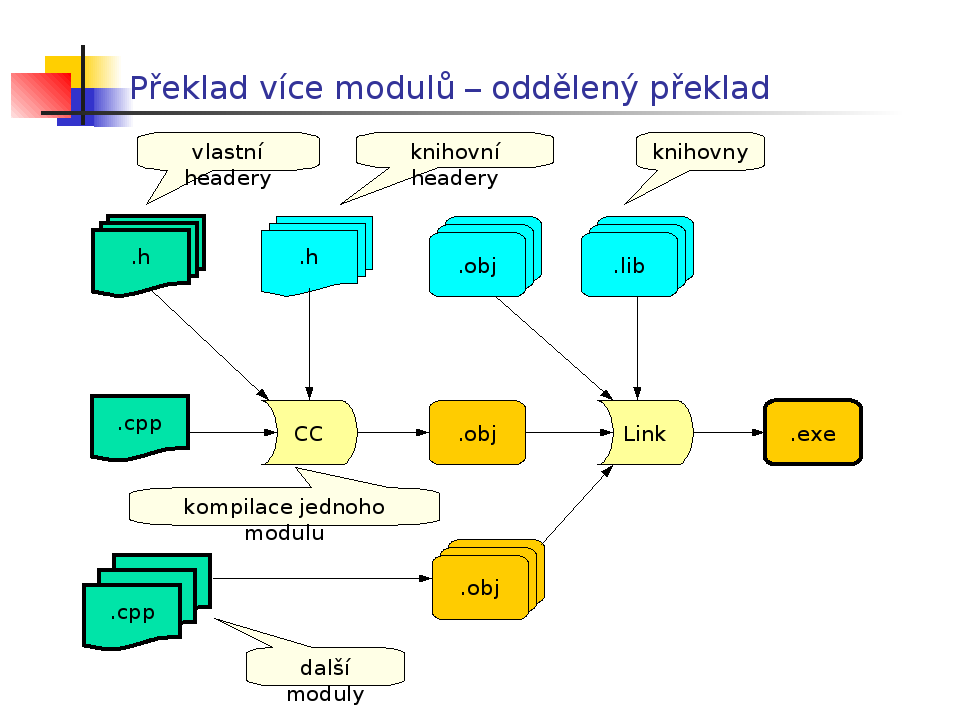
\includegraphics[width=10cm]{informatika/programovanie/obrazky/oddelenypreklad02.png}\end{center}
Smysl odděleného překladu modulů je urychlení celkového překladu -- nepřekládat to, co se od minula nezměnilo. Oddělený překlad dnes díky automatizaci makefily (viz níže) a integrovanými prostředími není téměř pro programátora vidět.

...pri tomto slide je vhodné ujasniť si, ako funguje statické a dynamické linkovanie (ako, kde a kedy sa opravujú adresy objektov atď.):
\begin{pitemize}
    \item \emph{Statické linkování} \\ Po odděleném překladu jednotlivé object moduly ještě neobsahují přímo adresy všech funkcí a externích identifikátorů, jen odkazy na ně. Linker se postará o jejich spojení dohromady. Je nutné, aby jména byla unikátní, takže u přetížených a virtuálních funkcí, jako je v C++, musí bý jména zpotvořena tak, aby ukazovala i třídu, namespace, parametry a jejich typy. To má na starosti compiler a říká se tomu \emph{name mangling}.
    \item \emph{Dynamické linkování} \\ Nastává po volání operačního systému -- zavedení dynamické knihovny do paměti. Jsou dvě možnosti jeho provedení, první je právě při zavádění knihovny, kdy se odkazy na všechny funkce (a mezi nimi navzájem) naplní správnými hodnotami (podle bázové adresy, na kterou se knihovna do paměti nahraje). Druhá možnost je použití dvou pointerů při volání funkcí z knihovny -- to se vytvoří tabulka skutečných adres, na kterou se z knihovny ukazuje. První možnost trvá déle při zavádění knihovny, druhá je zase pomalejší při provádění, ale umožňuje kód knihovny beze změn sdílet více procesy.
\end{pitemize}


\par\begin{center}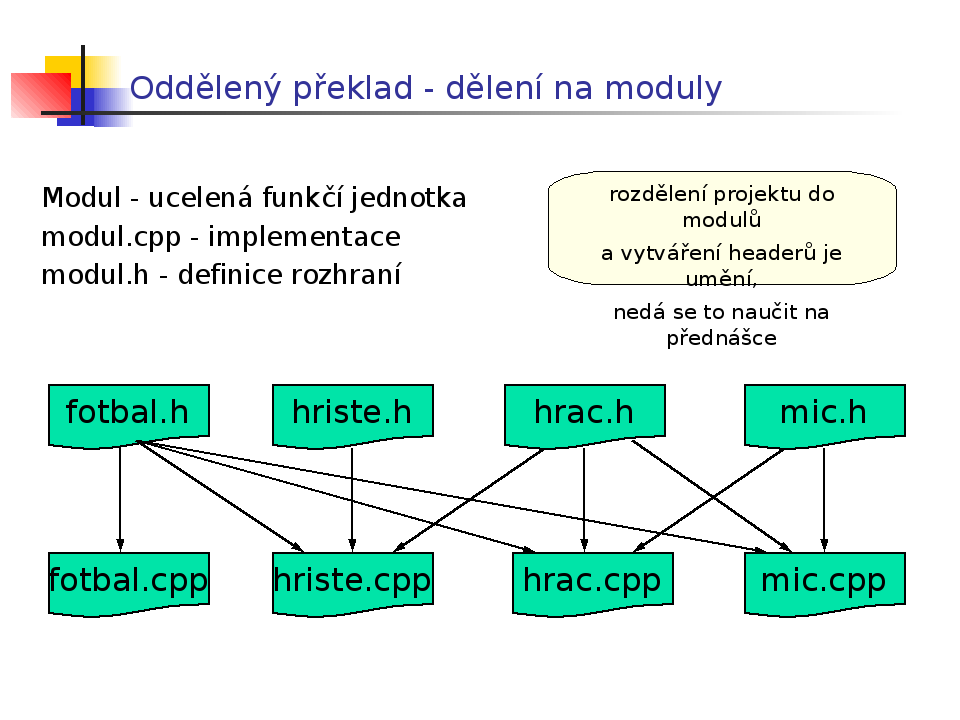
\includegraphics[width=10cm]{informatika/programovanie/obrazky/oddelenypreklad03.png}\end{center}

\emph{Linker} je program, který prijímá jeden alebo více objektů generovaných kompilátorem a složí je v jeden spustitelný program.

Objektový kód, nebo objektový soubor je reprezentace kódu, který kompilátor nebo assembler vytvoří zpracováním zdrojového kódu. Objektové soubory obsahují kompaktní kód, často nazývaný \uv{binárky} :-) Linker se typicky používá na vytvoření spustitelnýho souboru nebo knihovny spojením (slinkováním) objektových souborů. Základní častí objektového souboru je strojový kód (kód přimo vykonávaný CPU počítače).

\subsubsection*{Makefile}

Smyslem programu \emph{make} je řízení překladu a linkování. Popis závislostí jednotlivých modulů a hlavičkových na sobě je definován v 1 textovém souboru -- \emph{Makefile} (tj. které soubory je nutné mít aktuální/vytvořené pro překlad kterého souboru). Make vždy po změně souboru přeloží jen to, co na něm závisí.
Formát souboru make:
\begin{verbatim}
targets: files; 
        commands; #comment; line-begin\
        line contd.;
\end{verbatim}
Targets -- cíle činností / cílové soubory, možno definovat vic, při spuštění make bez parametrů se bere první; univ. nástroj (nejen pro překlad C/C++). Lze definovat i vlastní makra (příkazem \texttt{<název makra> = <string>}) a pak je používat (\texttt{\$\{makro\}}).

\subsection{Neprocedurální programování, logické programování}

\subsubsection*{Neprocedurální programování}
\emph{Deklarativní programování} je postaveno na paradigmatu, podle něhož je program založen na tom, co se počítá a ne jak se to počítá. Je zde deklarován vstup a výstup a celý program je chápán jako funkce vyhodnocující vstupy podávající jediný výstup. Například i webovské stránky jsou deklarativní protože popisují, jak by stránka měla vypadat -- titulek, font, text a obrázky -- ale nepopisují, jak konkrétně zobrazit stránky na obrazovce.

\emph{Logické programování} a \emph{funkcionální programování} jsou poddruhy deklarativního programování. Logické programování využívá programování založené na vyhodnocování vzorů - tvrzení a cílů. Klasickým zástupcem jazyka pro podporu tohoto stylu je Prolog.

Tento přístup patří pod deklarativní programování stejně jako funkcionální programování, neboť deklaruje, co je vstupem a co výstupem, a nezabývá se jak výpočet probíhá. Naopak program jako posloupnost příkazů je paradigma imperativní.

\emph{Funkcionální programování} patří mezi deklarativní programovací principy.

Alonzo Church vytvořil formální výpočtový model nazvaný $\lambda$-kalkul. Tento model slouží jako základ pro funkcionální jazyky. Funkcionální jazyky dělíme na:
\begin{pitemize}
	\item typované - Haskell
	\item netypované - Lisp, Scheme
\end{pitemize}

Výpočtem funkcionálního programu je posloupnost vzájemně ekvivalentních výrazů, které se postupně zjednodušují. Výsledkem výpočtu je výraz v normální formě, tedy dále nezjednodušitelný. Program je chápán jako jedna funkce obsahující vstupní parametry mající jediný výstup. Tato funkce pak může být dále rozložitelná na podfunkce.

\subsubsection*{Prolog}

Prolog je logický programovací jazyk. Název Prolog pochází z francouzského programmation en logique (\uv{logické programování}). Byl vytvořen Alainem Colmerauerem v roce 1972 jako pokus vytvořit programovací jazyk, který by umožňoval vyjadřování v logice místo psaní počítačových instrukcí. Prolog patří mezi tzv. deklarativní programovací jazyky, ve kterých programátor popisuje pouze cíl výpočtu, přičemž přesný postup, jakým se k výsledku program dostane, je ponechán na libovůli systému.

Prolog je využíván především v oboru umělé inteligence a v počítačové lingvistice (obzvláště zpracování přirozeného jazyka, pro nějž byl původně navržen). Syntaxe jazyka je velice jednoduchá a snadno použitelná pravě proto, že byl původně určen pro počítačově nepříliš gramotné lingvisty.

Prolog je založen na \emph{predikátové logice prvního řádu} (konkrétně se omezuje na Hornovy klauzule). Běh programu je pak představován aplikací dokazovacích technik na zadané klauzule. Základními využívanými přístupy jsou \emph{unifikace}, \emph{rekurze} a \emph{backtracking}.

Interpret Prologu se snaží nalézt nejobecnější substituci, která splní daný cíl - tzn. nesubstituuje zbytečně, pokud nemusí (použití interních proměnných -- \_123 atd.). Za dvě proměnné může být substituována jedna interní proměnná (např. při hledání svislé úsečky -- konstantní X souřadnice) -- tomu se říká \emph{unifikace} proměnných. Pro proměnnou, jejíž hodnota může být libovolná, se v prologu užívá znak \uv{\_}. 

Datové typy v prologu se nazývají \emph{termy}. Základním datovým typem jsou \emph{atomy} (začínají malým písmenem, nebo se skládají ze speciálních znaků (\texttt{+ - * / \dots}, nebo jsou to znakové řetězce (\texttt{'text'})). Dále \uv{jsou} v prologu čísla (v komerčních implementacích i reálná), proměnné (velké písmeno) a struktury (definované rekursivně - pomocí funktoru dané arity a příslušným počtem termů, které jsou jeho argumenty -- \texttt{okamzik(datum(1,1,1999),cas(10,10))}). Posledním typem proměnných jsou seznamy, které jsou probírány později.

\medskip\textbf{Základní principy}:

Programování v Prologu se výrazně liší od programování v běžných procedurálních jazycích jako např. C. Program v prologu je databáze faktů a pravidel (dohromady se faktům a pravidlům paradoxně říká procedury), nad kterými je možno klást dotazy formou tvrzení, u kterých Prolog zhodnocuje jejich pravdivost (dokazatelnost z údajů obsažených v databázi).

Například lze do databáze uložit fakt, že Monika je dívka:
\begin{verbatim}
dívka(monika).
\end{verbatim}

Poté lze dokazatelnost tohoto faktu prověřit otázkou, na kterou Prolog odpoví yes (ano):
\begin{verbatim}
?- dívka(monika).
     yes.
\end{verbatim}

Také se lze zeptat na všechny objekty, o kterých je známo, že jsou dívky (středníkem požadujeme další výsledky):
\begin{verbatim}
?- dívka(X).
     X = monika;
     no.
\end{verbatim}

Pravidla (závislosti) se zapisují pomocí implikací, např.
\begin{verbatim}
syn(A,B) :- rodič(B,A), muž(A).
\end{verbatim}

Tedy: pokud B je rodičem A a zároveň je A muž, pak A je synem B. První části pravidla (tj. důsledku) se říká hlava a všemu co následuje za symbolem \texttt{:-} (tedy podmínkám, nutným pro splnění hlavy) se říká tělo. Podmínky ke splnění mohou být odděleny buď čárkou (pak jde o konjunkci, musejí být splněny všechny), nebo středníkem (disjunkce), přičemž čárky mají větší prioritu.

\medskip\textbf{Příklad}:

Typickou ukázkou základů programování v Prologu jsou rodinné vztahy.
\begin{verbatim}
sourozenec(X,Y) :- rodič(Z,X), rodič(Z,Y).
rodič(X,Y) :- otec(X,Y).
rodič(X,Y) :- matka(X,Y).
muž(X) :- otec(X,_).
žena(X) :- matka(X,_).
matka(marie,monika).
otec(jiří,monika).
otec(jiří,marek).
otec(michal,tomáš).
\end{verbatim}

Prázdný seznam je označen atomem $[]$, neprázdný se tvoří pomocí funktoru \texttt{'.'} (tečka) - \texttt{.(Hlava,Tělo)}. V praxi se to (naštěstí ;-)) takhle složitě rekurzivně zapisovat nemusí, stačí napsat \texttt{[a,b,c...]}, resp \texttt{[Začátek | Tělo]}, kde začátek je výčet prvků (ne seznam) stojících na začátku definovaného seznamu, a tělo je (rekurzivně) seznam (např. \texttt{[a,b,c|[]]}).

Aritmetické výrazy se samy o sobě nevyhodnocují, dokud jim to někdo nepřikáže. Takže např. predikát \texttt{5*1 = 5} by selhal. Vyhodnocení se vynucuje pomocí operátoru \emph{is} (pomocí = by došlo jen k unifikaci) - není to ale ekvivalent \uv{\texttt{=}} z jiných jazyků. Tento operátor se musí použít na nějakou volnou proměnnou a aritmetický výraz, s jehož hodnotou bude tato proměnná dále svázaná (jako např. \texttt{X is 5*1,X=5} uspěje).

Důležitý je i \emph{operátor řezu} (značíme vykřičníkem). Tento predikát okamžitě uspěje, ale při tom zakáže backtrackování přes sebe zpět. (\texttt{prvek1(X,[X|L]):-!. prvek1(X,[\_|L]):-prvek1(X,L).} - je-li prvek nalezen, je zakázán návrat = najde jen první výskyt prvku). Dále je důležitá negace (\texttt{not(P):- P, !, fail. not(P).} -- uspěje, pokud se nepodaří cíl P splnit). Řez tedy umožňuje ovlivňovat efektivitu prologovských programů, definovat vzájemně se vylučující použití jednotlivých klauzulí procedury, definovat negaci atd.

\subsubsection*{Haskell}
Haskell je standardizovaný funkcionální programovací jazyk používající zkrácené vyhodnocování, pojmenovaný na počest logika Haskella Curryho. Byl vytvořen v 80. letech 20. století. Posledním polooficiálním standardem je Haskell 98, který definuje minimální a přenositelnou verzi jazyka využitelnou k výuce nebo jako základ dalších rozšíření. Jazyk se rychle vyvíjí, především díky svým implementacím Hugs a GHC (viz níže).

Haskell je jazyk dodržující \emph{referenční transparentnost}. To, zjednodušeně řečeno, znamená, že tentýž (pod)výraz má na jakémkoliv místě v programu stejnou hodnotu. Mezi další výhody tohoto jazyka patří přísné \emph{typování proměnných}, které programátorovi může usnadnit odhalování chyb v programu. Haskell plně podporuje práci se soubory i standardními vstupy a výstupy, která je ale poměrně složitá kvůli zachování referenční transparentnosti. Jako takový se Haskell hodí hlavně pro algoritmicky náročné úlohy minimalizující interakci s uživatelem.

\medskip\textbf{Příklady}:

Definice funkce faktoriálu:
\begin{verbatim}
fac 0 = 1
fac n = n * fac (n - 1)
\end{verbatim}

Jiná definice faktoriálu (používá funkci product ze standardní knihovny Haskellu):
\begin{verbatim}
fac n = product [1..n]
\end{verbatim}

Naivní implementace funkce vracející n-tý prvek Fibonacciho posloupnosti:
\begin{verbatim}
fib 0 = 0 
fib 1 = 1 
fib n = fib (n - 2) + fib (n - 1)
\end{verbatim}

Elegantní zápis řadícího algoritmu quicksort:
\begin{verbatim}
qsort [] = []
qsort (pivot:tail) = 
  qsort left ++ [pivot] ++ qsort right
  where
    left = [y | y <- tail, y < pivot]
    right = [y | y <- tail, y >= pivot]
\end{verbatim}

TODO: popsat stráže (případy, otherwise), seznamy, řetězení, pattern matching u parametrů funkcí, lok. definice (where, let) -- patří to sem?

\subsubsection*{Lisp}

Lisp je funkcionální programovací jazyk s dlouhou historií. Jeho název je zkratka pro List processing (zpracování seznamů). Dnes se stále používá v oboru umělé inteligence. Nic ale nebrání ho použít i pro jiné účely. Používá ho například textový editor Emacs, GIMP či konstrukční program AutoCAD.

Další jazyky od něj odvozené jsou například Tcl, Smalltalk nebo Scheme.


\medskip\textbf{Syntaxe}:
Nejzákladnějším zápisem v Lispu je seznam. Zapisujeme ho jako:
\begin{verbatim}
(1 2 "ahoj" 13.2)
\end{verbatim}

Tento seznam obsahuje čtyři prvky:
\begin{pitemize}
	\item celé číslo 1
	\item celé číslo 2
	\item text \uv{ahoj}
	\item reálné číslo 13,2
\end{pitemize}

Jde tedy o uspořádanou čtveřici. Všimněte si, že závorky nefungují tak jako v matematice, ale pouze označují začátek a konec seznamu. Seznamy jsou v Lispu implementovány jako binární strom degenerovaný na jednosměrně vázaný seznam. Co se seznamem Lisp udělá, záleží na okolnostech.

\textbf{Příkazy}: Příkazy píšeme také jako seznam, první prvek seznamu je však název příkazu. Například sčítání provádíme příkazem +, což interpreteru zadáme takto:
\begin{verbatim}
(+ 1 2 3)
\end{verbatim}
Interpretr odpoví 6.

\textbf{Ukázka kódu}:
Program hello world lze zapsat několika způsoby. Nejjednoduší vypadá takto:
\begin{verbatim}
(format t "Hello, World!")
\end{verbatim}

Funkce se v Lispu definují pomocí klíčového slova defun:
\begin{verbatim}
(defun hello ()
        (format t "Hello, World!")
)
(hello)
\end{verbatim}

Na prvních dvou řádcích je definice funkce hello, na třetím řádku je tato funkce svým jménem zavolána.
Funkcím lze předávat i argumenty. V následujícím příkladu je ukázka funkce fact, která vypočítá faktoriál zadaného čísla:
\begin{verbatim}
(defun fact (n)
        (if (= n 0)
                1
                (* n (fact (- n 1)))
        )
)
\end{verbatim}
Pro výpočet faktoriálu čísla 6 předáme tuto hodnotu jako argument funkci fact:
\begin{verbatim}
(fact 6)
\end{verbatim}
Návratovou hodnotou funkce bude hodnota 720.

\subsubsection*{Logické programování}
TODO (není součástí otázek pro obor Programování)

\subsection{Struktura překladače, lexikální, syntaktická analýza}

Zdroj: poznámky a slidy z přednášek Principy překladačů Dr. J. Yaghoba

\subsubsection*{Překladače}

\begin{definiceN}{Překladač}
Formální definice: \emph{překladač} je zobrazení $L_{in}\to L_{out}$ pro nějaké dva jazyky $L_{in},L_{out}$, vstupní generovaný gramatikou $G_{in}$, výstupní generovaný gramatikou $G_{out}$ nebo přijímaný automatem $A_{out}$. Je to takové zobrazení, kde $\forall w\in L_{in}\ \exists w'\in L_{out}$. Pro $w\notin L_{in}$ zobrazení neexistuje.

Neformálně jde o stroj, který nějaký zdrojový kód (v nějakém zdrojovém jazyce) převádí na cílový kód (v cílovém jazyce) a případně vypisuje chybová hlášení.

Definice neříká nic o třídách jazyků a gramatik, ve kterých překladač operuje. Běžné programovací jazyky jsou \uv{plus minus} bezkontextové -- nebo se na bezkontextové převádějí, aby byly rozpoznatelné něčím prakticky implementovatelným (tedy zásobníkovým automatem, Turingovy stroje jsou poněkud složité).
\end{definiceN}


\begin{priklady}
Příklady použití překladačů:
\begin{pitemize}
    \item (překvapivě) překlad programů, psaných v nějakém vyšším programovacím jazyce, do strojového kódu cílové platformy
    \item syntax-highlighting (většinou lexikálně řízený)
    \item pretty printer
    \item statické kontroly programu (hledání chyb bez spouštění programů)
    \item interpretery (např. skriptovacích jazyků, run-time moduly pro interpretované jazyky jako je Java)
    \item databázové stroje, dotazovací jazyky
\end{pitemize}
\end{priklady}


\begin{obecne}{Překlad programu}
Program (pro jednoduchost jediný modul) se 
\begin{penumerate}
    \item ze zdrojového kódu v nějakém programovacím jazyce \emph{preprocesorem} (což je taky překladač, upravující zdrojový kód na textové úrovni) převede na textový soubor (připravený pro další překlad),
    \item \emph{překladačem} se převede dál do assemblerového kódu (jde o kód v jiném jazyce, mnohem bližším cílové architektuře -- jde o textový popis instrukcí procesoru),
    \item \emph{assemblerem} se převádí na \uv{object-file} -- modul, ve kterém už jazyk odpovídá strojovému kódu cílové CPU,
    \item nakonec \emph{linker}, resp. \emph{loader} připojí další informace a vytvoří finální spustitelný kód.
\end{penumerate}
\end{obecne}

\begin{obecne}{Fáze překladu překladačem}
Tradičně se překladače dělí na dvě fáze -- \emph{front-end} a \emph{back-end}. První z nich je zaměřená hlavně na analýzu zdrojového kódu po lexikální a syntaktické stránce a její převod do nějakého mezikódu, tj. přípravu pro back-end. Úkolem back-endu je pak z předpřipravené formy vygenerovat finální kód v cílovém jazyce.

První fáze se dále dělí na tyto části:
\begin{penumerate}
    \item \emph{lexikální analýza} -- převádí vstupní text do binární formy, na sled identifikátorů a konstant; hodnoty objektů ukládá do spec. tabulek 
    \item \emph{syntaktická analýza} -- abstraktní část, nezajímá se o hodnoty a význam elementů jazyka, úkolem je rozpoznat, zda vstupní slovo (vstup) patří do jazyka; v dnešních překladačích staví tzv. \uv{syntaktický strom} kódu
    \item \emph{sémantická analýza} -- zkoumá sémantiku (význam, smysl) elementů jazyka (např. u sčítání proměnných kontrola typů, používání definovaných proměnných atd.)
    \item \emph{generování mezikódu} -- úzce svázané se sémantickou analýzou, načítá hodnoty lexikálních elementů z tabulek a vytváří binární formu kódu, v ideálním případě nezávislou na vstupním ani výstupním jazyce
    \item \emph{optimalizace nad mezikódem} -- díky překladu do nějakého abstraktního mezikódu lze nad ním potom provádět různé obecné (teoreticky dokázané) optimalizace, aby byl výsledný kód ekvivalentní s původním, ale rychlejší při provádění cílovým strojem
\end{penumerate}

Backend má na starosti hlavně
\begin{penumerate}
    \item \emph{generování kódu} -- vytváří už kód pro konkrétní cílový stroj / architekturu / CPU. 
    \item \emph{optimalizace nízkoúrovňového kódu} -- optimalizace, zaměřené na vlastnosti konkrétních CPU a cílový jazyk (tj. takové, které nad obecným mezikódem s vysokou abstrakcí provést nejde)
\end{penumerate}

Všechny fáze překladače (většinou, když se pominou třeba staší verze GCC a podobně) sdílejí jednotné \emph{tabulky symbolů} -- hodnot lexikálních elementů a jiných věcí a obsluhu chyb. Překladač musí rozpoznat všechny chyby, ale bez velké časové režie, navíc nesmí mít falešné poplachy. Taky by neměl vyrábět chyby sám ;-).

V dřívějších překladačích se vstupní kód procházel několikrát, protože nebylo technicky možné ho udržet celý v paměti. Dnes je potřeba většinou jen jeden přechod, ale někdy je nutných víc (např. dopředné skoky v assembleru -- nevím ještě jak daleko skáču).
\end{obecne}

\begin{poznamkaN}{Syntax-driven compilation}
Nejdůležitější částí dnešních překladačů bývá syntaktická analýza; provádí se často najednou se sémantickou analýzou a generováním mezikódu -- vše mívá na starosti jediný zásobníkový automat. Navíc si často sám vyvolává lexikální analýzu, ta je jím tedy řízená, takže se taková technika označuje \emph{syntaxí řízený překlad}.
\end{poznamkaN}

\begin{obecne}{Automatické generování (částí) překladače}
Protože dnešní programovací jazyky jsou relativně složité (gramatiky které je generují mají řádově stovky přepisovacích pravidel), konstrukce automatů přijímajících takové jazyky \uv{ručně} je příliš náročná. Proto existují nástroje, které generují některé části překladače -- generátor lexikálních analyzátorů -- \uv{scannerů} -- (popíšu lexikální elementy a struktury a co s nimi dělá a vypadne mi analyzátor jako kód v jazyce C) je např. \emph{Flex}, pro výrobu parserů (syntaktických analyzátorů) z popisu gramatiky slouží např. \emph{Bison}, \emph{Coco/R} nebo \emph{ANTLR}. Některé známé překladače mají ale i tak ručně generované parsery (GCC).

Existují i generátory generátorů kódu (ale jejich méně, protože to je dost složité) -- pro popis výstupního CPU dostanu z instrukčního mezikódu kód přímo pro něj. Instrukční mezikód může být pro více architektur úplně stejný. Příkladem tohoto je \emph{Mono JIT Compiler}.
\end{obecne}


\begin{obecne}{Mezikód}
(Vysokoúrovňový) \emph{mezikód} je vlastně jakési rozhraní pro přechod (rozdělení i spolupráci) mezi front-endem a back-endem. Jde o binární reprezentaci zdrojového kódu, má být nezávislý na vstupním i výstupním jazyce. Pokud tomu tak je, je možné např. kombinovat různé back-endy a front-endy, jako tomu je u GCC (více back-endů pro 1 front-end) nebo .NET (více front-endů). Většinou ale je mezikód o něco posunutý buď více k závislosti na back-endu nebo na front-endu.

Mezikód je možné reprezentovat několika způsoby -- např. syntaktickým stromem (vhodné v paměti), postfixovým zápisem (linearizace stromu) nebo tříadresovým kódem (lineární, sekvence příkazů $x:= y\ \mathrm{op}\ z$).
\end{obecne}

\begin{obecne}{Graf toku řízení}
Graf toku řízení je graf, vytvářený překladači (větš. pro 1 funkci) za účelem optimalizací a také generování výsledného kódu. Uzly -- \emph{základní bloky} -- jsou nepřerušované výpočty (bez instrukcí skoků a bez cílů skoků uvnitř bloků), z nichž první instrukce bývá cílem skoku nebo vstupním bodem funkce. Hrany pak reprezentují skoky -- pro podmíněné skoky a case příkazy pak z uzlů vede více hran.
\end{obecne}

\subsubsection*{Lexikální analýza}

\begin{definiceN}{Lexikální analýza}
Lexikální analýza je část překladače, zodpovědná za rozpoznávání jednotlivých nedělitelných elementů zdrojového jazyka (např. klíčová slova, identifikátory, závorky atd.) a jejich převod na nějakou binární reprezentaci, vhodnou pro syntaktickou analýzu (např. uložení názvů identifikátorů do tabulek symbolů). V zásadě jde o rozpoznávání regulárních výrazů. Historicky šlo o provedení analýzy na celém zdrojáku a přeposlání do další fáze, dnes je většinou ovládaná ze syntaktické analýzy (opakované volání \uv{vrať další element}). Slouží také ke zvětšení \uv{výhledu} dalších fází (jedním elementem přestává být jeden znak, je jím jeden element vstupního jazyka).
\end{definiceN}

\begin{definiceN}{Token, pattern}
\emph{Token} je výstup lexikální analýzy -- jeden nedělitelný element zdrojového jazyka. Je zároveň vstupem syntaktické analýzy (tam se nazývá \emph{terminál}). Lexikální analýza uvažuje množinu řetězců, které produkují pro syntaktickou analýzu stejný token (např. díky ignore-caseovosti nebo jako důsledek sloučení všech řetězcových nebo číselných konstant pod stejný token, protože s nimi je dále nakládáno bez ohledu na hodnotu). Množina řetězců, produkujících daný token, se popisuje urč. pravidly -- \emph{patternem}, kde se obvykle užívá regulárních výrazů.
\end{definiceN}

\begin{definiceN}{Lexém}
\emph{Lexém} neboli \emph{lexikální element} je sekvence znaků ve zdrojovém kódu, která (většinou) odpovídá nějakému patternu nějakého tokenu. Např. komentáře ale jako svůj výstup žádný token nemají.
\end{definiceN}

\begin{definiceN}{Literál}
\emph{Literál} je konstanta ve vstupním jazyce -- má svoji hodnotu (atribut), ukládanou do tabulek symbolů.
\end{definiceN}

\begin{poznamkaN}{Atributy tokenů}
Je-li jeden token rozpoznáván více patterny, nebo je-li to literál, má nějaké další atributy (většinou jenom jeden), které jeho význam upřesňují -- např. token \uv{relační operátor} má zpřesnění \uv{menší nebo rovno}, token \uv{číselný literál} má zpřesnění \uv{12345}.
\end{poznamkaN}

\begin{obecne}{Problémy lex. analýzy}
Mezi některé problémy, které syntaktická analýza musí řešit, patří
\begin{pitemize}
    \item Počítání zarovnání -- některé jazyky (Python) mají zarovnání na řádce jako svoji syntaktickou konstrukci
    \item Identifikátory s mezerami (rozlišit identifikátor od jiné konstrukce, i víceslovné)
    \item Klíčová slova jako identifikátory (někdy se mohou překrývat)
    \item Kontextově závislé tokeny -- token závisí na jiných informacích (např. \texttt{a*b;} v C -- jde o násobení, nebo deklaraci pointerové proměnné), tady je nutné tokeny slučovat pro oba významy ???
\end{pitemize}
\end{obecne}

\begin{obecne}{Pozadí lex. analýzy}
Na pozadí lexikálního analyzátoru většinou pracuje nějaký konečný automat (protože rozpoznávání regulárních výrazů -- hodnotou reg. výrazu je reg. jazyk -- je práce pro konečné automaty). Po každém rozpoznaném tokenu je potřeba automat uvést zpět do výchozího stavu.
\end{obecne}

\begin{obecne}{Lexikální chyby}
Chyba v lexikální analýze nastane tehdy, když konečný automat nemůže pokračovat dál a není v koncovém stavu (např. pokud nalezne neplatný znak, nebo neukončený řetězec na konci řádky apod.). Většina lexikálních analyzátorů (pomineme Turbo Pascal ;-)) by měla být schopna nějakého \uv{rozumného} zotavení z chyby -- vypsat chybu a domyslet chybějící znak nebo neplatný znak ignorovat apod., tj. nezastavit se na první chybě. I logické zotavení může ale scanner úplně rozhodit a ten pak vyhazuje nesmyslné chyby. Je také spousta chyb, které lexikální analýza nepozná a projeví se až u syntaktické analýzy, např. \texttt{beign} místo \texttt{begin}, chápané jako identifikátor. 
\end{obecne}

\begin{poznamkaN}{Bufferování vstupu}
Syntaktická analýza časově zabere cca 60-80\% překladu, takže se pro její urychlení používá bufferování -- nečte se po znacích, ale o něco napřed. Problémem pak jsou např. \texttt{\#include} direktivy (jsou-li ve vstupním jazyce) -- v okamžiku vložení jiného souboru je scanner v nějakém stavu apod.; scannery musí mít pak možnost přepínat mezi více vstupními soubory (manipulovat s několika buffery).
\end{poznamkaN}

\subsubsection*{Syntaktická analýza}

\begin{definiceN}{Syntaktická analýza}
Syntaktická analýza je část překladače, zodpovědná za:
\begin{penumerate}
    \item rozhodnutí, zda dané slovo (vstup) patří do zpracovávaného jazyka
    \item syntaxí řízený překlad
    \item stavbu derivačního stromu (nalezení přepisovacích pravidel ze startovacího neterminálu gramatiky na vstupní posloupnost tokenů -- terminálů)
\end{penumerate}

Většina programovacích jazyků je bezkontextová, proto je syntaktická analýza představována zásobníkovým automatem. Syntaktická analýza operuje s gramatikou daného jazyka (snaží se o přepis abstraktních neterminálů na terminály -- tokeny jazyka).
\end{definiceN}

\begin{definiceN}{Derivační strom}
Derivační strom je \uv{grafická} reprezentace slova vstupního jazyka, nebo spíše derivací, které bylo potřeba provést, aby se v gramatice startovací symbol přepsal na dané slovo (posloupnost terminálů). Uzly takového grafu jsou neterminály i terminály gramatiky jazyka (v listech ale jsou jen terminály, ve vnitřních uzlech neterminály). Hrany grafu představují přepsání podle pravidla gramatiky -- vedou od neterminálu který se přepisuje, ke všem neterminálům nebo terminálům na které se přepisuje (mluvíme o bezkontextových gramatikách, takže na levé straně stojí jen jeden neterminál).

Přepsání v gramatice bohužel nemusí být jednoznačné (tj. pro stejnou posloupnost neterminálů existuje více platných derivačních stromů). Přikladem je problém \uv{dangling else} z jazyků typu Pascal nebo C -- mám-li za sebou 2x \texttt{if-then} a pak jedno \texttt{else}, nemusí být (z gramatiky) jasné, ke kterému \texttt{if-then} ono \texttt{else} patří. Takové problémy lze (a je nutné) odstranit převodem na jednoznačnou gramatiku (např. přes další neterminál).
\end{definiceN}

\begin{obecne}{Levá rekurze, levá faktorizace, nebezkontextovost}
Levá rekurze v gramatice se objevuje, pokud je v ní neterminál $A$, pro který platí $A\Rightarrow^{*} A\alpha$ pro nějaké $\alpha\neq\lambda$. Tj. přes $A$ je možné projít kolikrát chci a vytvořit posloupnost $\alpha\alpha\dots$. Pokud parser začíná u startovacího neterminálu a hledá derivace na na terminály \uv{shora dolů} (to jeden z druhů scannerů dělá), neví jakou hloubku rekurze má použít. Proto je nutné i levou rekurzi, stejně jako nejednoznačnosti, z gramatiky napřed odstranit její úpravou (zde opět pomůže přechod přes nový neterminál).

Problémem je i levá faktorizace -- případ, kdy se v gramatice vyskytují pravidla jako $A\to \alpha\beta$ a zároveň $A\to \alpha\gamma$. I ten je možné řešit úpravou gramatiky (přenos rozhodnutí na pozdější dobu, kdy bude známo, který ze symbolů $\beta,\gamma$ si vybrat).

Může se také i pro běžné konstrukce z programovacích jazyků stát, že nevyhovují bezkontextovým gramatikám -- např. kontrola deklarace identifikátoru před použitím, kontrola počtu parametrů funkce apod. Zde syntaktická analýza bezkontextovým způsobem nestačí a tyto případy je třeba řešit jinak.
\end{obecne}

\begin{definiceN}{Názvosloví gramatik, FIRST a FOLLOW}
Gramatiky se v teorii překladačů označují dvěma až třemi znaky a číslem v závorce, obecně ve tvaru $PXY(k)$, kde:
\begin{pitemize}
    \item $X$ je směr čtení vstupu (V našem případě vždy $L$, tj. zleva doprava),
    \item $Y$ jsou druhy derivace ($L$ – levé, $R$ – pravé derivace),
    \item $P$ označuje prefix (ještě jemnější dělení na třídy u některých gramatik) a
    \item $k$ představuje \emph{výhled} (lookahead), každý parser totiž vidí jen na jeden nebo několik tokenů dopředu a další neuvažuje. Obvykle je to celé číslo, většinou 1, ale také 0 nebo obecně $k$.
\end{pitemize}
Příklady: $LL(1), LR(0), LR(1), LL(k), SLR(1), LALR(1)$

Množiny \emph{FIRST} a \emph{FOLLOW} představují množinu použitelných neterminálů na urč. místech (začátky řetězců derivovaných z nějakého pravidla, resp. řetězce které mohou následovat po nějakém neterminálu) a používají se pro konstrukci parserových automatů pro nějakou gramatiku.
\end{definiceN}

TODO: formalizovat FIRST a FOLLOW, neni to moc slozite?

\begin{definiceN}{Analýza shora dolů}
Analýza shora dolů je technika parserů, kdy se parser snaží najít nejlevější derivaci pro vstupní řetězec. Pokouší se tedy zkonstruovat derivační strom pro daný vstup počínaje kořenem a přidáváním uzlů do stromu -- rozhoduje se, podle kterého pravidla gramatiky přepíše. Pravidlo pro odstranění nejednoznačnosti je provádění \emph{jen levých derivací}, proto pak automatům vadí levá rekurze a musí se odstraňovat. Techniky pro nalezení přepisovacího pravidla jsou:
\begin{pitemize}
    \item \emph{Rekurzivní sestup} pomocí procedur -- pro každý neterminál existuje jedna procedura, která se rozhodne, které pravidlo použije na základě výhledu. Pro rozhodování se sestavují množiny FIRST a FOLLOW každého neterminálu. Potom musí zkontrolovat, jestli pravá strana tohoto pravidla odpovídá vstupu (přičemž výskyt neterminálu na pravé straně znamená zavolání jemu příslušné procedury).     
    \item \emph{Nerekurzivní analýza s predikcí} -- je implementováno automatem s explicitním zásobníkem: ten má \emph{parsovací tabulku}, která se liší podle gramatiky (sama práce automatu je vždy stejná) -- jsou v ní řádky odpovídající neterminálům a sloupce terminálům, v políčkách jsou přepisovací pravidla  nebo chyby. Na zásobník automatu se ukládají symboly gramatiky a ze vstupu se čtou (lineárně terminály). V každém kroku se automat rozhodne podle vstupu a vrcholu zásobníku -- je-li tam terminál, vyhodí se a ukazatel vstupu se posune (nebo se skončí); je-li na zásobníku neterminál, rozhoduje se podle tabulky (položka určená vstupem a neterminálem, buďto se použije přepisovací pravidlo nebo skončí chybou). Konstrukce tabulky je opět závislá na množinách FIRST a FOLLOW.
\end{pitemize}
Analýza shora dolů je používána v parserech jednoduchých jazyků ($LL(1)$ gramatiky s řešením konfliktů zvětšením výhledu na $k$ terminálů) -- v generátorech parserů ANTLR a Coco/R, například.
\end{definiceN}

\begin{definiceN}{Analýza zdola nahoru, LR automat}
Parsery s analýzou zdola nahoru se pokoušejí najít pozpátku nejpravější derivaci pro vstupní řetězec -- zkonstruovat derivační strom pro daný vstup počínaje listy a stavěním zespodu až po kořen stromu. V jednom redukčním kroku je tak podřetězec odpovídající pravé straně pravidla gramatiky nahrazen neterminálem z levé strany pravidla. Analýza zdola nahoru se používá ve např. v generátoru parserů Bison -– je schopná vytvořit parsery pro $LALR(1), GLR(1)$ gramatiky, které jsou oproti $LL(1)$ parserům \uv{silnější} (Třída rozpoznávaných jazyků LR(1) je vlastní nadmnožina LL(1)), všechny běžné programovací jazyky zapsatelné bezkontextovou gramatikou sem patří. Navíc se dá implementovat zhruba stejně efektivně jako metoda shora dolů.

V analýze zdola nahoru se používá nějaký zásobníkový automat (\emph{LR automat}) čtoucí ze vstupu, parametrizovaný tabulkami \emph{ACTION} a \emph{GOTO}. Na zásobníku se pak uchovávají stavy a symboly gramatiky (nebo jen stavy). Vrchol zásobníku představuje aktuální stav. V počáteční konfiguraci je pointer vstupu nastavený na začátek a na zásobníku je počáteční stav. V každém kroku podle stavu a tokenu na vstupu adresuji tabulku ACTION a získám akci k provedení:
\begin{pitemize}
    \item \emph{SHIFT} $s$ -- posune vstup o 1 terminál, který přidá na zásobník spolu s novým stavem $s$.
    \item \emph{REDUCE} $A\to\alpha$ -- zruší ze zásobníku tolik dvojic stavů a symbolů, jak dlouhé je $\alpha$, na zásobník dá $A$ a stav, který najde v tabulce GOTO na pozici odpovídající neterminálu $A$ a aktuálnímu stavu
    \item \emph{ACCEPT} -- generuje nějaký výstup, slovo je úspěšně rozpoznáno
    \item \emph{ERROR} -- zahlásí chybu
\end{pitemize}
V LR automatech v klidu projdou i gramatiky s levou rekurzí. Obecně se v nich používají nějaké $LR(k)$ gramatiky, většinou \uv{rozšířené} -- doplněné o \uv{tečky}, ukazatele pozice v pravidlech, které pomáhají s rozpoznáním konce vstupu. Ke konstrukci tabulek ACTION a GOTO jsou opět potřeba množiny FIRST a FOLLOW, nyní rozšířené na $k$ symbolů.
\end{definiceN}


TODO: přidat popis LR(1) a LALR(1) gramatik?

\subsection{Interpretované jazyky, virtuální stroje}

\subsubsection*{Interpretovaný jazyk}

Zdrojový jazyk se nepřekládá do kódu skutečného procesoru, ale do kódu nějakého abstraktního stroje... Interpret přeložený do kódu skutečného stroje simuluje zvolený abstraktní stroj.

Důvodem může být např. málo prostoru pro překladač (8-bity a BASIC), nebo přenositelnost -- stejný abstraktní stroj může běžet na různých OS i různých architekturách CPU (AS/400, Java).

Tato metoda má i problémy:

\begin{pitemize}
	\item Problém s rychlostí - dá se řešit pomocí JIT (Just-In-Time compilation): Pokud interpret narazí na kód abstraktního stroje, který ještě není přeložen, okamžitě ho přeloží na kód cílového stroje a uloží si ho vedle do své cache
	\item Problémy s přenositelností - nevhodné změny v chování abstraktního stroje mohou přivodit problémy s přenositelností (Java)
	\item Jak zvolit abstraktní stroj - aby pokryl chování všech zdrojových jazyků (např .NET)
\end{pitemize}

\begin{obecne}{Použití dynamické paměti v interpretovaných jazycích}
Pokud je dynamická paměť podporována, pak výhradně s garbage collectorem, protože:
\begin{pitemize}
	\item Ukazatele jsou pod kontrolou
	\item Snadnější programování
	\item Rychlejší práce s dynamickou pamětí (program obvykle nepotřebuje tolik paměti, aby GC vůbec musel zasahovat, takže se pouze souvisle alokuje; simulátor abstraktního ale obvykle zabere více paměti, než by musel)
\end{pitemize}
\end{obecne}

\subsubsection*{Zo \uv{starých} textov :-)}

In computer programming an emph{interpreted language} is a programming language whose implementation often takes the form of an interpreter. Theoretically, any language may be compiled or interpreted, so this designation is applied purely because of common implementation practice and not some underlying property of a language.

Many languages have been implemented using both compilers and interpreters, including Lisp, C, BASIC, and Python. While Java and C\# are translated to a form that is intended to be interpreted, just-in-time compilation is often used to generate machine code.

An \emph{interpreter} is a computer program that essentially compiles and executes (interprets) another computer program "on-the-fly" at runtime.

In computer science the term "interpreter" is sometimes used instead of the term emulator. There are software interpreters and hardware interpreters. We will denote interpreter as a software interpreter. It can also refer to a program that performs compilation as well as emulation. Most interpreters available today generally compile source code when the code is first encountered during program execution, rather than in a separate phase prior to execution.

An interpreter has a number of advantages over a compiler, including:
\begin{pitemize}
	\item because it can be tailored to a specific programming language making it simpler to implement and more compact (BASIC was supported on many early home computers for this reason).
	\item it allows program implementation to be independent of the characteristics of the host cpu (the Java interpreter is a good example of this).
\end{pitemize}

The main disadvantage of interpreters is that when a program is interpreted, it runs slower than if it had been compiled. The difference in speeds could be tiny or great; often an order of magnitude and sometimes more.

\medskip\textbf{Bytecode interpreter}

There is a spectrum of possibilities between interpreting and compiling, depending on the amount of analysis performed before the program is executed. For example, Emacs Lisp is compiled to bytecode, which is a highly compressed and optimized representation of the Lisp source, but is not machine code (and therefore not tied to any particular hardware). This "compiled" code is then interpreted by a bytecode interpreter (itself written in C). The compiled code in this case is machine code for a virtual machine, which is implemented not in hardware, but in the bytecode interpreter. The same approach is used with the Forth code used in Open Firmware systems: the source language is compiled into "F code" (a bytecode), which is then interpreted by an architecture-independent virtual machine.

\medskip\textbf{Just-in-time compilation}

Just-in-time compilation, or JIT, refers to a technique where bytecode is compiled to native machine code at runtime; giving the high execution speed of running native code at the cost of increased startup-time as the bytecode is compiled. It has gained attention in recent years, which further blurs the distinction between interpreters, byte-code interpreters and compilation. JIT is available for both the .NET and Java platforms. The JIT technique is a few decades old, appearing in languages such as Smalltalk in the 1980s.

In computer science, a \emph{virtual machine} is software that creates a virtualized environment between the computer platform and its operating system, so that the end user can operate software on an abstract machine.

The original meaning of virtual machine, sometimes called a hardware virtual machine, is that of a number of discrete identical execution environments on a single computer, each of which runs an operating system (OS).

Another meaning of virtual machine is a piece of computer software that isolates the application being used by the user from the computer.

A Java Virtual Machine (JVM) is a set of computer software programs and data structures which implements a specific virtual machine model. This model accepts a form of computer intermediate language, commonly referred to as Java bytecode, which conceptually represents the instruction set of a stack-oriented, capability architecture. This code is most often generated by Java language compilers, although the JVM can also be targeted by compilers of other languages. JVMs using the "Java" trademark may be developed by other companies as long as they adhere to the JVM standard published by Sun (and related contractual obligations).

\subsection{Pojmy a principy objektov�ho n�vrhu}

TODO: tohle je tup� copy \& paste z Wikipedie, p�ed�lat/p�elo�it

\begin{e}{Definice}{0}{Objektov� n�vrh}
Object oriented design is part of OO methodology and it forces programmers to think in terms of objects, rather than procedures, when they plan their code. An object contains encapsulated data and procedures grouped together to represent an entity. The 'object interface', how the object can be interacted, is also defined. An object oriented program is described by the interaction of these objects. Object Oriented Design is the discipline of defining the objects and their interactions to solve a business problem that was identified and documented during object oriented analysis.
\end{e}

\begin{obecne}{Uva�ovan� aspekty pro objektov� n�vrh (prerekvizity)}
\begin{pitemize}
    \item \emph{Conceptual model (must have):} Conceptual model is the result of object-oriented analysis, it captures concepts in the problem domain. The conceptual model is explicitly chosen to be independent of implementation details, such as concurrency or data storage.
    \item \emph{Use case (must have):} Use case is description of sequences of events that, taken together, lead to a system doing something useful. Each use case provides one or more scenarios that convey how the system should interact with the users called actors to achieve a specific business goal or function. Use case actors may be end users or other systems.
    \item \emph{System Sequence Diagram (should have):} System Sequence diagram (SSD) is a picture that shows, for a particular scenario of a use case, the events that external actors generate, their order, and possible inter-system events.
    \item \emph{User interface documentations (if applicable):} Document that shows and describes the look and feel of the end product's user interface. This is not mandatory to have, but helps to visualize the end-product and such helps the designer.
    \item \emph{Relational data model (if applicable):} A data model is an abstract model that describes how data is represented and used. If not object database is used, usually the relational data model should be created before the design can start. How the relational to object mapping is done is included to the OO design.
\end{pitemize}
\end{obecne}

\begin{e}{Pozn�mka}{0}{0}
Objektov� n�vrh po��t� s vlastnostmi objektov�ho programov�n�, podporovan�mi objektov�-orientovan�mi jazyky. Jsou to zejm�na:
\begin{pitemize}
    \item zapouzd�en�, objekty
    \item abstrakce, skryt� informac�
    \item d�di�nost
    \item vn�j�� interface
    \item polymorfismus
\end{pitemize}
\end{e}

\begin{obecne}{Postup p�i objektov�m n�vrhu / Designing concepts}
\begin{pitemize}
    \item Defining objects, creating class diagram from conceptual diagram: Usually map entity to class.
    \item Identifying attributes.
    \item Use design patterns (if applicable): A design pattern is not a finished design, it is a description of a solution to a common problem. The main advantage of using a design pattern is that it can be reused in multiple applications. It can also be thought of as a template for how to solve a problem that can be used in many different situations and/or applications. Object-oriented design patterns typically show relationships and interactions between classes or objects, without specifying the final application classes or objects that are involved.
    \item Define application framework (if applicable): Application framework is a term usually used to refer to a set of libraries or classes that are used to implement the standard structure of an application for a specific operating system. By bundling a large amount of reusable code into a framework, much time is saved for the developer, since he/she is saved the task of rewriting large amounts of standard code for each new application that is developed.
    \item Identify persisted objects/data (if applicable): Identify objects that have to be persisted. If relational database is used design the object relation mapping.
    \item Identify, define remote objects (if applicable)
\end{pitemize}
\end{obecne}

\begin{obecne}{V�stup, v�sledek objektov�ho n�vrhu / Output (deliverables) of object oriented design}
\begin{pitemize}
    \item Class diagram: Class diagram is a type of static structure diagram that describes the structure of a system by showing the system's classes, their attributes, and the relationships between the classes.
    \item Sequence diagram: Expend the System Sequence Diagram to add specific objects that handle the system events. Usually we create sequence diagram for important and complex system events, not for simple or trivial ones. A sequence diagram shows, as parallel vertical lines, different processes or objects that live simultaneously, and, as horizontal arrows, the messages exchanged between them, in the order in which they occur.
\end{pitemize}
\end{obecne}



\subsection{Generick� programov�n� � �ablony a generika}

Z�kladn� my�lenkou, kter� se skr�v� za pojmem generick� programov�n�, je rozd�len� k�du programu na algoritmus a datov� typy takov�m zp�sobem, aby bylo mo�n� z�pis k�du algoritmu ch�pat jako obecn�, bez ohledu na to, nad jak�mi datov�mi typy pracuje. Konkr�tn� k�d algoritmu se z n�j st�v� dosazen�m datov�ho typu.

U kompilovan�ch jazyk� doch�z� k rozvinut� k�du v dob� p�ekladu. Typick�m p��kladem jazyka, kter� podporuje tuto formu generick�ho programov�n�, je jazyk C++. Mechanismem, kter� zde generick� programov�n� umo��uje, 
jsou takzvan� �ablony (templates).

\medskip
\begin{poznamkaN}{Metaprogramov�n� a Generika}
It differs from normal programming in that it somehow invokes within the language a metaprogramming facility. Because it happens as an extension of the language, new semantics are introduced and the language is enriched in this process. It is closely related to metaprogramming, but does not involve the generation of source code (none, at least, that is visible to the user of the language). It is different from programming with macros as well, as the latter refers to textual search-and-replace and is not part of the grammar of the language but implemented by a pre-processor. One exception to this is the macro facility in Common Lisp, in which macros operate on parse trees rather than text.

Oby�ejn� fce maj� p�ednost p�ed generick�mi???
\end{poznamkaN}

\begin{definiceN}{�ablony}
Template metaprogramming is a metaprogramming technique in which templates are used by a compiler to generate temporary source code, which is merged by the compiler with the rest of the source code and then compiled. The output of these templates include compile-time constants, data structures, and complete functions. The use of templates can be thought of as compile-time execution. The technique is used by a number of languages, the best-known being C++, but also Curl, D, and XL.
\end{definiceN}

\begin{prikladN}{T��da parametrizovan� typem (kontejner)}
As an example of the benefits of generic programming, when creating containers of objects it is common to write specific implementations for each datatype contained, even if the code is virtually identical except for different datatypes. Instead, a possible declaration using generic programming could be to define a template class (using the C++ idiom):
\begin{verbatim}
  template<typename T> 
  class List 
  { 
    T x;
    List<T> *next;
  };
  
  List<Animal> list_of_animals;
  List<Car> list_of_cars;
  
  ...
  
  conductor = root;
  while ( conductor != NULL ) {
    cout<< conductor->x;
    conductor = conductor->next;
  }
\end{verbatim}
Above T represents the type to be instantiated. The list generated is then treated as a list of whichever type is specified. These "containers-of-type-T", commonly called generics, are a generic programming technique that allows the defining of a class that takes and contains different datatypes (not to be confused with polymorphism, which is the algorithmic usage of exchangeable sub-classes) as long as certain contracts such as subtypes and signature are kept. Although the example above is the most common use of generic programming, and some languages implement only this aspect of it, generic programming as a concept is not limited to generics. 
\end{prikladN}

\begin{prikladN}{Typov� nez�visl� funkce}
Another applicaton is type-independent functions as in the Swap example below:
\begin{verbatim}
  template<typename T>
  void Swap(T & a, T & b) //"&" passes parameters by reference
  {
     T temp = b;
     b = a;
     a = temp;
  }
  
  string hello = "world!", world = "Hello, ";
  Swap( world, hello );
  cout << hello << world << endl; //Output is "Hello, world!"
\end{verbatim}
\end{prikladN}

\begin{prikladN}{Faktori�l pomoc� �ablon}
\begin{verbatim}
  template <int N>
  struct Factorial 
  {
      enum { value = N * Factorial<N - 1>::value };
  };
   
  template <>
  struct Factorial<0> 
  {
      enum { value = 1 };
  };
   
  // pou�it�:
  int x = Factorial<4>::value; // == 24
  int y = Factorial<0>::value; // == 1
\end{verbatim}
\end{prikladN}


\begin{prikladN}{traits}
Programovac� paradigma vyu��vaj�c� �ablony, ze kter�ch nejsou vytv��eny objekty. Ur�eny k dopln�n� informac� o n�jak�m typu.
\\\\Obsahuj� pouze:
\begin{pitemize}
\item Definice typ�
\item Statick� funkce
\end{pitemize}

\begin{verbatim}
  template< typename T > 
  struct is_void{ 
    static const bool value = false;
  };
  
  template<> 
  struct is_void< void >{ 
    static const bool value = true; 
  };
  
  // pou�it�:
  is_void<int>::value; // false
  is_void<void>::value; // true
\end{verbatim}
\end{prikladN}
\newpage
\begin{prikladN}{policy classes}
Ur�eny k definov�n� ur�it�ho chov�n�. Jous to t��dy, ze kter�ch obvykle nejsou vytv��eny objekty a jsou p�ed�v�ny jako parametr �ablon�m. Defaultn� hodnotou parametru �asto b�v� �ablona traits. Hlavn� spojen� s C++ (v ostatn�ch jazyc�ch se zat�m neroz���ilo).
\begin{verbatim}
  template < typename output_policy, typename language_policy >
  class HelloWorld : public output_policy, public language_policy
  {
      using output_policy::Print;
      using language_policy::Message;
       
      public: void Run() //behaviour method
      {
          //two policy methods
          Print( Message() );
      }
  };
   
  class OutputPolicy_WriteToCout
  {
   protected:
      template< typename message_type >
      void Print( message_type message )
      {
          std::cout << message << std::endl;
      }
  };
   
  class LanguagePolicy_English
  {
      protected: std::string Message() { return "Hello, World!"; }
  };
   
  class LanguagePolicy_German
  {
      protected: std::string Message() { return "Hallo Welt!"; }
  };
   
  int main()
  {
      /* example 1 */
      HelloWorld<OutputPolicy_WriteToCout, LanguagePolicy_English>  hello_world;
      hello_world.Run(); // Prints "Hello, World!"
   
     /* example 2 
      * does the same but uses another policy, the language has changed
      */
      HelloWorld<OutputPolicy_WriteToCout, LanguagePolicy_German> hello_world2;
      hello_world2.Run(); // Prints "Hallo Welt!"
  }
\end{verbatim}
\end{prikladN}
\newpage
\begin{definiceN}{Dynamick� (run-time) polymorfismus}
D�d�n� + VMT = flexibilita.
P��padn� jeho varianta s �ablonami:
\begin{verbatim}
class Base
{
public:
    virtual void method() { std::cout << "Base"; }
    virtual ~Base() {}
};
 
class Derived : public Base
{
public:
    virtual void method() { std::cout << "Derived"; }
};
 
int main()
{
    Base *pBase = new Derived;
    pBase->method(); //outputs "Derived"
    delete pBase;
    return 0;
}
\end{verbatim}
\end{definiceN}

\begin{definiceN}{Statick� (compile-time) polymorfismus}
Je p�et�ov�n� fukc� a oper�tor�, �e�� se p�i kompilaci = rychlost.
P��padn� jeho varianta s �ablonami:
\begin{verbatim}
template <class Derived>
struct base
{
    void interface()
    {
         // ...
         static_cast<Derived*>(this)->implementation();
         // ...
    }
};
 
struct derived : base<derived>
{
     void implementation();
};
\end{verbatim}
Lze tak dos�hnout podobn�ch v�c� jako s VMT.
\end{definiceN}

\begin{obecne}{Pou�it� v programovac�ch jazyc�ch}
The template construct of C++ used in the examples above is widely cited as the generic programming construct that popularized the notion among programmers and language designers and provides full support for all generic programming idioms. D also offers fully generic-capable templates based on the C++ precedent but with a simplified syntax. Java has provided generic programming facilities syntactically based on C++'s since the introduction of J2SE 5.0 and implements the generics, or "containers-of-type-T", subset of generic programming.
\end{obecne}

\begin{reportN}{IP 21.6.2011} Co je to generick� programov�n�, k �emu se pou��v� a v �em spo��vaj� jeho v�hody?

Napi�te stru�nou implementaci generick� t��dy List nebo HashTable.

Popi�te implementaci v C++ a Jav� (asi by sta�il i C#, ale v zad�n� byla explicitn� napsan� java).
\end{reportN}

\begin{reportN}{IP 21.6.2011 ($<$2007)} Popiste sablony
\\Jak jsou implementovany (popiste jak jsou implementovany v C++ nebo Java) (to som teda fakt netusil)
\end{reportN}

\begin{reportN}{IOI 21.6.2011 ($<$2007)}
Co je to generick� programov�n�, k �emu se pou��v� a v �em spo��vaj� jeho v�hody?

Napi�te stru�nou implementaci generick� t��dy List nebo HashTable.
\end{reportN}

\begin{reportN}{Yaghob}
Co je to traits a policy classes, co je to statick� polymorfismus apod. Nakonec jsem to n�jak vymyslel a shodli jsme se na tom, �e to v�m, tak�e taky za 1.
\end{reportN}

\subsection{N�vrhov� vzory}

N�vrhov� vzor je pojmenovan� a popsan� �e�en� typick�ho probl�mu. Princip existuj� u� dlouho: v architektu�e -- nap�. barokn� styl, literatura -- tragick� hrdina, romantick� novela\dots

V software se mnoh� postupy \uv{vynal�zaj�} st�le znovu -- n�vrhov� vzory maj� potom pro typickou situaci popisovat:
\begin{pitemize}
	\item jak a kdy maj� b�t objekty vytv��eny
	\item jak� vztahy a struktury maj� obsahovat t��dy
	\item jak� chov�n� maj� m�t t��dy, jak maj� spolupracovat objekty
\end{pitemize}

N�vrhov� vzor (design pattern) je tedy obecn� znovupou�iteln� �e�en� probl�m� �asto se vyskytuj�c�ch p�i n�vrhu softwaru. Nejedn� se o hotov� design, kter� by se dal transformovat p��mo na k�d -- je to v�cem�n� jen popis nebo �ablona, jak �e�it n�jak� probl�m vyskytuj�c� se ve v�ce r�zn�ch situac�ch. Objektov�-orientovan� n�vrhov� vzory typicky ukazuj� vztahy a interakce mezi t��dami nebo objekty -- bez specifikace konkr�tn�ch kone�n�ch t��d nebo objekt�. Algoritmy nejsou pova�ov�ny za n�vrhov� vzory, proto�e �e�� sp�e v�po�etn� probl�my ne� designov�.

Ne v�echny softwarov� vzory (software patterns) jsou n�vrhov�. N�vrhov� vzory �e�� probl�my na �rovni n�vrhu softwaru (software desing). Jin� druhy vzor� (jako nap�. architektur�ln� vzory (architectural patterns)) popisuj� probl�my a �e�en�, kter� se zam��uj� na jin� �rovn�.

Z�kladn� prvky n�vrhov�ch vzor�:
\begin{pitemize}
	\item \emph{N�zev} -- co nejv�ce vystihuj�c� podstatu, usnadn�n� komunikace -- spole�n� slovn�k
	\item \emph{Probl�m} -- obecn� situace kterou m� NV �e�it
	\item \emph{Podm�nky} -- popis okolnost� ovliv�uj�c�ch pou�it� NV a kontextu vhodn�m pro pou�it�; n�kter� okolnosti mohou b�t vyu�ity p�i �e�en�, jin� naopak jsou v konfliktu
	\item \emph{�e�en�} -- soubor pravidel a vztah� popisuj�c�ch jak dos�hnout �e�en� probl�mu; nejen statick� struktura, ale i dynamika chov�n�
	\item \emph{Souvislosti a d�sledky} -- detailn� vysv�tlen� pou�it�, implementace a principu fungov�n�; zp�sob pr�ce s NV v praxi
	\item \emph{P��klady} -- definice konkr�tn�ho probl�mu, vstupn� podm�nky, popis implementace a v�sledek
	\item \emph{Souvisej�c� vzory} -- pou�it� jednoho NV nep�edstavuje typicky ucelen� �e�en� -- �et�zec NV
\end{pitemize}

\ramcek{14.5cm}{
\emph{Nasleduj�ce sa vyu�uje na predmete N�vrhov� vzory, ktor� je odpor��an� a� pre nmgr �t�dium}:\par
	Kategorie z�kladn�ch NV:
	\par\begin{center}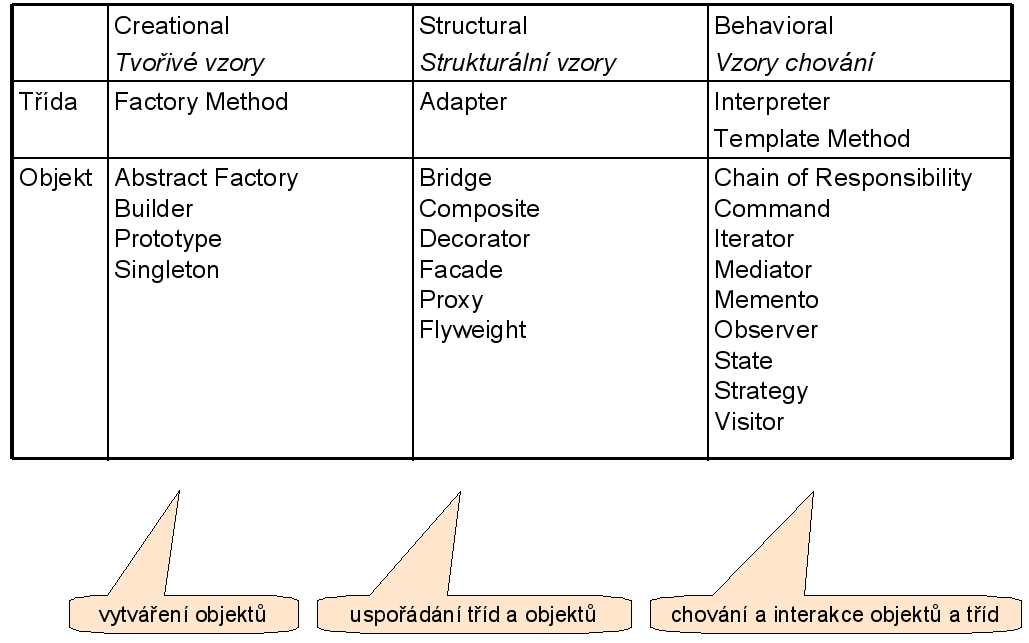
\includegraphics[width=12cm]{informatika/programovanie/obrazky/designpatterns.png}\end{center}
	
	N�vrhov� vzory je mo�no klasifikovat dle probl�m� kter� �e��. Pr�klady klasifikace vzor� podle �e�en�ch probl�m�:
	\begin{pitemize}
		\item \emph{Fundamental patterns}: ??? nevyhod�me to, je to jen na wiki a nepopsane
		\item \emph{Creation patterns}: vytv��en� objekt�
		\item \emph{Structural patterns}: jak jsou t��dy a objekty slo�en� do v�t��ch struktur
		\item \emph{Behavioral patterns}: rozd�len� funk�nosti a zodpov�dnosti mezi objekty; komunikace mezi objekty; umo��uje zam��it se p�i n�vrhu na propojen� t��d, ne na b�hov� detaily
		\item \emph{Concurrency patterns} ??? tohle taky
	\end{pitemize}
}

\begin{e}{P��klady}{0}{0}
Creational patterns:
\begin{pitemize}
    \item Factory method (zaji��uje rozhodnut� o typu vytv��en�ho objektu p�i polymorfismu)
    \item Prototype (jak klonovat objekty)
    \item Singleton (jak omezit objekt jen na 1 instanci)
\end{pitemize}

Structural patterns:
\begin{pitemize}
    \item Adapter (konverze rozhran� objekt�)
    \item Bridge (odd�len� rozhran� a implementace t��dy)
    \item Composite (jak slo�it v�ce objekt� do jednoho s jednotn�m p��stupem)
    \item Proxy (jak zajistit p��stup k jin�mu objektu p�es m�j objekt)
    \item Decorator (jak zm�nit vlastnosti t��dy nebo zajistit roz���enou funk�nost bez odd��ov�n�)
\end{pitemize}

Behavioral patterns:
\begin{pitemize}
    \item Chain of responsibility (jak ur�it kdo vykon� akci, kdy� z venku p�ijde po�adavek)
    \item Command (odst�n�n� klienta od zpracov�n� po�adavku -- klient neur�uje kdy a jak se to provede)
    \item Iterator (projit� prvk� pole bez znalosti jejich implementace)
    \item Visitor (nav�t�ven� v�ech objekt� n�jak� struktury a pr�ce s nimi, aby v�echny nemusely implementovat stejn� metody (a m�nit se p�i jejich zm�n�))
    \item Template (jak mohou odvozen� t��dy ovliv�ovat algoritmy b�zov� t��dy)
\end{pitemize}
\end{e}


TODO: roz��ri�, doplni�, opravi� :-)


\section{Architektura počítačů a operačních systémů}
\begin{pozadavky}
\begin{pitemize}
\item Architektury počítače
\item Procesory, multiprocesory
\item Sběrnice, protokoly
\item Vstupní a výstupní zařízení
\item Architektury OS
\item Vztah OS a HW, obsluha přerušení
\item Procesy, vlákna, plánování
\item Synchronizační primitiva, vzájemné vyloučení
\item Zablokování a zotavení z něj
\item Organizace paměti, alokační algoritmy
\item Principy virtuální paměti, stránkování, algoritmy pro výměnu stránek, výpadek stránky, stránkovací tabulky, segmentace
\item Systémy souborů, adresářové struktury
\item Bezpečnost, autentifikace, autorizace, přístupová práva
\item Druhy útoků a obrana proti nim
\item Kryptografické algoritmy a protokoly
\end{pitemize}
\end{pozadavky}
\subsection{Architektury po��ta�e}

\begin{e}{Definice}{0}{Architektura po��ta�a}
Architektura po��ta�a popisuje \uv{v�etko, �o by mal vedie� ten, ktor� programuje v assembleri / tvor� opera�n� syst�m}. Teda:
\begin{pitemize}
        \item z ak�ch �ast� -- �trukt�ra po��ta�a, usporadanie
        \item v�znam �ast� -- funkcia �asti, ich vn�torn� �trukt�ra
        \item ako spolu �asti komunikuj� -- riadenie komuk�cie
        \item ako sa jednotliv� �asti ovl�daj�, ak� je ich funk�nos� navonok
\end{pitemize}
\end{e}

\begin{e}{Definice}{0}{V�ce�rov�ov� organizace po��ta�e}
\begin{pitemize}
        \item Mikroprogramov� �rove� (priamo technick� vybavenie po��ta�a)
        \item Strojov� jazyk po��ta�e (virtu�lny stroj nad obvodov�m rie�en�m; vybavenie~-- popis architekt�ry a organiz�cie)
        \item �rove� opera�n�ho syst�mu (doplnenie predch�dzaj�cej �rovne o s�bor makroin�trukci� a nov� organiz�ciu pam�ti)
        \item �rove� assembleru (najni��ia �rove� �udsky orientovan�ho jazyka)
        \item �rove� vy���ch programovac�ch jazyk� (obecn� alebo probl�movo orientovan�; prv� nestrojovo orientovan� �rove�)
        \item �rove� aplika�n�ch program�
\end{pitemize}
\end{e}


\begin{obecne}{Je teda potrebn� definova�}
\begin{pitemize}
        \item In�truk�n� s�bor (defin�cia prechodovej funkcie medzi stavmi po��ta�a, form�t in�trukcie, sp�sob z�pisu, mo�nosti adresovania operandov)
        \item Registrov� model (rozli�ovanie registrov procesoru: pod�a vo�by, pomocou ur�enia registru~-- explicitn�/implicitn� register; pod�a funkcie registru~-- riadiaci~register/register~operandu)
        \item Definice specializovan�ch jednotek (jednotka na v�po�et vo floatoch;\\fetch/decode/execute jednotky)
        \item Paralelismy (rozklad na �lohy, ktor� sa daj� spracova� s��asne~-- granularita (programy, podprogramy, in�trukcie...))
        \item Stupe� predikce (schopnos� pripravi� sa na o�ak�van� udalos� (na��tanie in�trukcie, nastavenie prenosu d�t)~-- explicitn� predikcia, �tatistika, heuristiky, adapt�vna predikcia)

\bigskip
        \item Datov� struktury a reprezent�ciu d�t (sp�sob ulo�enia d�t v po��ta�i, mapovacie funkcie medzi re�lnym svetom a vn�torn�m ulo�en�m, minim�lna a maxim�lna ve�kos� adresovate�n� jednotky)
        \item Adresov� konvencie (ako sa pristupuje k d�tov�m �trukt�ram~-- \emph{segment+offset} alebo \emph{line�rna adres�cia}; ve�kos� pam�ti a jej ��rika, \uv{povolen�} miesta)

\bigskip
        \item ��zen� (spolupr�ca procesoru a ostatn�ch jednotiek, interakcia s okol�m, preru�enia~-- vn�torne/vonkaj�ie)
        \item Vstupy a v�stupy (met�dy prenosu d�t medzi procesorom a ostatn�mi jednotkami/po��ta�om a okol�m; zahr�uje defin�cie d�tov�ch �trukt�r, identifik�cia zdroja/cie�a, d�tov�ch ciest, protokoly, reakcie na chyby).
        \item ���e datov�ch cest
        \item Stupe� sd�len� (na �rovni obvodov~-- zdie�anie obvodov procesoru a IO; na �rovni jednotiek~-- zdie�anie ALU viacer�mi procesormi)
\end{pitemize}
\end{obecne}

\begin{obecne}{Z�kladn� definice}
  \begin{pitemize}
      \item \textbf{ALU} (tak� Processing Element) Aritmeticko-logick� jednotka - z�kladn� komponenta procesoru (2.z�kladn� je �adi�).  
      \item \textbf{�adi�} (Control Unit) je elektronick� ��dic� jednotka, realizovan� sekven�n�m obvodem, kter� ��d� �innost v�ech ��st� po��ta�e. Toto ��zen� je prov�d�no pomoc� ��dic�ch sign�l�, kter� jsou zas�l�ny jednotliv�m modul�m (d�l��m ��stem po��ta�e). Reakce na ��dic� sign�ly - stavy jednotliv�ch modul� - jsou naopak zas�l�ny zp�t �adi�i pomoc� stavov�ch hl�en�. D�l�� ��st� po��ta�e je nap�. hlavn� pam�, kter� rovn� obsahuje �adi�, kter� je pod��zen hlavn�mu �adi�i po��ta�e, jen� je sou��st� CPU.
      \item \textbf{Sb�rnice} (Bus) je sada dat.stream� propojuj�c� v�ce za��zen�. Instruction Stream (��zen� komunikace � po�adavky/potvrzen�, indikace typu dat na datov�ch vodi��ch) Data Stream (p�enos dat mezi zdrojov�m a c�lov�m za��zen�m, adresy, data, slo�it�j�� p��kazy     
      \end{pitemize} 
\end{obecne}

\subsubsection*{Flynn's taxonomy}

The taxonomy of computer systems proposed by M. J. Flynn in 1966 has remained the focal point in the field.
This is based on the notion of instruction and data streams that can be simultaneously manipulated by the
machine. A stream is just a sequence of items (instruction or data).

\begin{description}
\item[Single Instruction, Single Data stream (SISD)] -
    A sequential computer (Von Neumann) which exploits no parallelism in either the instruction or data streams. Single control unit (CU) fetches single Instruction Stream (IS) from memory. The CU then generates appropriate control signals to direct single processing element (PE or ALU) to operate on single Data Stream (DS) i.e. one operation at a time

Examples of SISD architecture are the traditional uniprocessor machines like a PC (currently manufactured PCs have multiple processors) or old mainframes.
  \begin{center}
    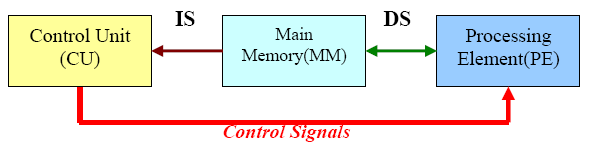
\includegraphics[width=10cm]{informatika/operacne_systemy_a_hw/obrazky/SISD.png}
  \end{center}

\item[Single Instruction, Multiple Data streams (SIMD)] -
    A computer which exploits multiple data streams against a single instruction stream to perform operations which may be naturally parallelized. For example, an array processor or GPU.
  \begin{center}
    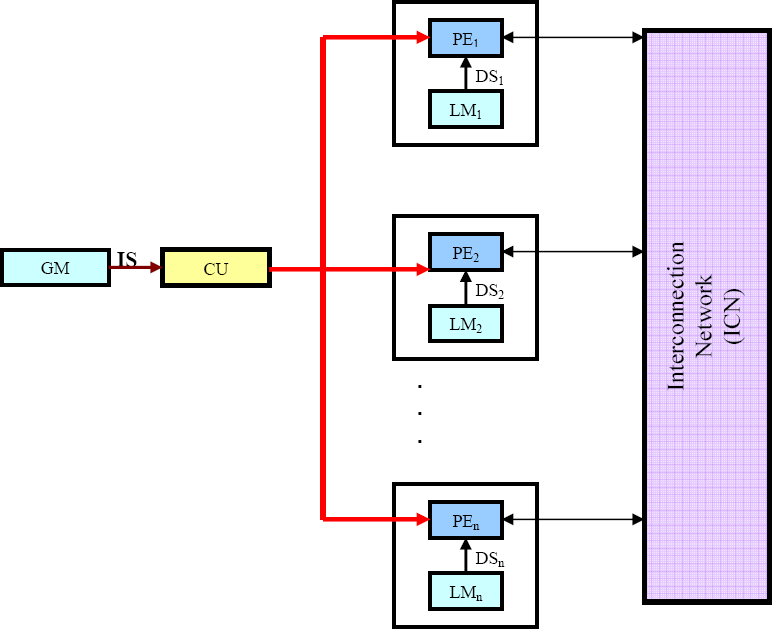
\includegraphics[width=12cm]{informatika/operacne_systemy_a_hw/obrazky/SIMD.png}
  \end{center}
  
\item[Multiple Instruction, Single Data stream (MISD)] -
    Multiple instructions operate on a single data stream. Uncommon architecture which is generally used for fault tolerance. Heterogeneous systems operate on the same data stream and must agree on the result. Examples include the Space Shuttle flight control computer.
  \begin{center}
    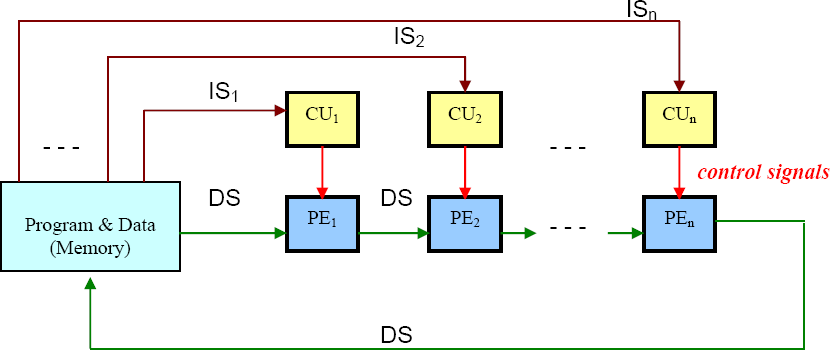
\includegraphics[width=12cm]{informatika/operacne_systemy_a_hw/obrazky/MISD.png}
  \end{center}
\item[Multiple Instruction, Multiple Data streams (MIMD)] -
    Multiple autonomous processors simultaneously executing different instructions on different data. Distributed systems are generally recognized to be MIMD architectures; either exploiting a single shared memory space or a distributed memory space. 

  \begin{center}
    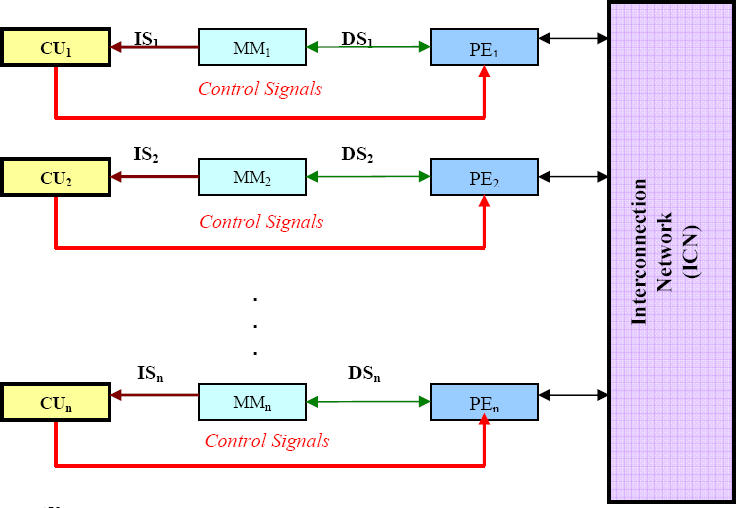
\includegraphics[width=12cm]{informatika/operacne_systemy_a_hw/obrazky/MIMD.png}
  \end{center}
\end{description}
\subsubsection*{Z�kladn� architektury po��ta��}

\begin{obecne}{Von Neumannova}
  \begin{pitemize}
      \item Po��ta� se skl�d� z ��d�c� jednotky, ALU, pam�ti a I/O jednotek
      \item �trukt�ra po��ta�a sa nemen� typom �lohy (tj. po��ta� je programovan� obsahem pam�ti). %to tuetschek sorry neumim cist... ajs
      \item Program se nejprve zavede do pam�ti, z n� se postupn� popo�ad� vyb�raj� instrukce (a n�sleduj�c� krok z�vis� na p�edchoz�m), po�ad� lze zm�nit instrukcemi skoku. 
      \item Do jedn� pam�ti, d�len� na bu�ky stejn� velikosti, se ukl�daj� i zpracov�van� data. Data jsou reprezentovan� bin�rn�. 
      \item V ka�d�m okam�iku je vykon�v�na jen jedna �innost. Je to architektura SISD (viz Flynnova taxonomie).
  \end{pitemize}

  Je pevn� dan� instruk�n� sada. Strojov� instrukce obsahuje opera�n� znak, kter� ur�uje druh operace, po�et parametr� atd., a operandov� ��st~-- um�stn�n� jednotliv�ch operand�. Vykonat jednu instrukci znamen�:
  \begin{pitemize}
          \item (fetch) na��ta� in�trukciu z pam�ti do procesoru
          \item (decode) zisti� o ak� in�trukciu ide
          \item (load) pripravi� zdrojov� operandy
          \item (execute) vykona� oper�ciu
          \item (store) ulozi� cie�ov� operandy
  \end{pitemize}

  P�i vykon�v�n� programu jsou pot�ebn� r�zn� registry~-- nejd�le�it�j�� jsou: PC (Program Counter, obsahuje adresu n�sleduj�c� instrukce), IR (Instruction Register, na�ten� instrukce pro zpracov�n� -- jm�no (typ) spolu s operandy (adresami)), SP (Stack Pointer, ukazatel na vrchol z�sobn�ku), MAR (memory access register~-- adresa do opera�n� pam�ti), MBR (memory buffer register, d�ta ��t�na/zapisov�na do pam�ti).

  Struktura jednoprocesorov�ho po��ta�e podle Von Neumanna:
  \begin{center}
    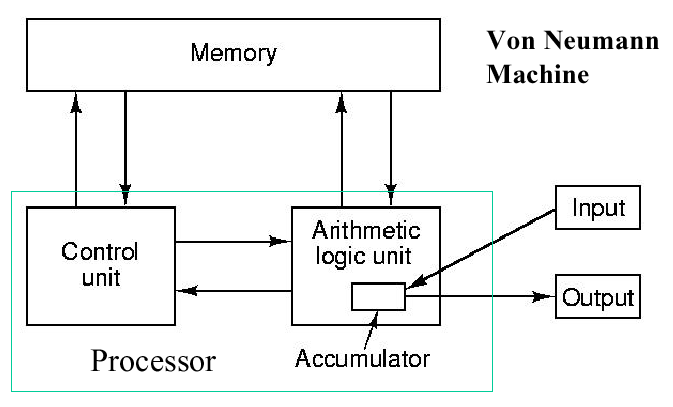
\includegraphics[width=8cm]{informatika/operacne_systemy_a_hw/obrazky/VonNeumann.png}
    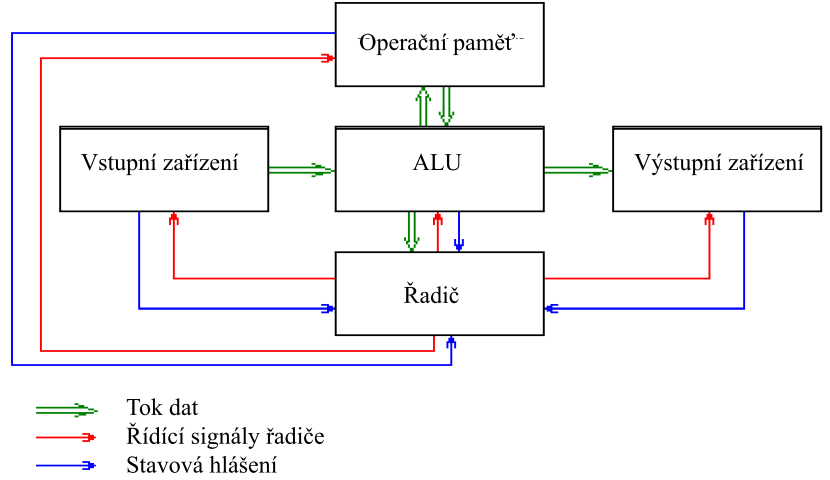
\includegraphics[width=8cm]{informatika/operacne_systemy_a_hw/obrazky/VonNeumann-Obdrzalek.png}
  \end{center}
\end{obecne}

\begin{description}
        \item[Control-flow]-- v�zna�n�m rysem von Neumannovy architektury je zp�sob prov�d�n�
programu. Strojov� instrukce, ze kter�ch se ka�d� p��mo spustiteln� program skl�d�, se prov�d�j� sekven�n�, jedna za druhou. Tedy ka�d� instrukce se provede tehdy, a� na ni dojde �ada, a nad takov�mi daty, jak� jsou pr�v� k dispozici. 
        \item[Data-flow (architektura ��zen� daty)]-- Alternativa k Control-flow. Okam�ik proveden� ur�it� akce se ��d� p�ipravenost� v�ech dat, kter� jsou k proveden� ur�it� akce zapot�eb�. V�hodou je mo�nost prov�d�t v�ce �innost� soub�n� - tedy v�t�� potenci�l paralelismu, kter� von Neumannov� koncepci naopak chyb�.
\end{description}

\begin{obecne}{Harvardsk�}
Vytvo�ena a� po Von Neumannov�, li�� se hlavn� t�m, �e program se ukl�d� do jin� pam�ti ne� data (tzn. jsou 2 \uv{druhy pam�ti}~-- instrukc� a dat). P��kladem jsou DSP procesory a mikrokontrolery. 

Nap�. AVR od Atmelu, a PIC~-- maj� pam� na program a data a RISC instruk�n� sadu; v�hoda odd�len�ch pam�t� je, �e m��ou m�t r�znou bitovou hloubku~-- 8 bitov� data, ale 12-, 14- �i 16- bitov� instrukce - nap�. ARM mus� ob�as pou��t v�ce ne� jednou instrukci na zpracov�n� obsahu pln� velikosti).

Oproti Von Neumannov� nehroz� nebezpe�� p�eps�n� programu sebou sam�m, ale kv�li v�t��mu po�tu pam�ov�ch sb�rnic je n�ro�n�j�� na v�robu. Pam� nav�c nelze d�lit podle pot�eby (rozd�len� je u� dan�).
\end{obecne}

\begin{e}{P��klad}{0}{Na�rtn�te typickou architekturu pocitace, ze kter� bude zrejm� um�st�n� a propojen� z�kladnich stavebn�ch prvku (procesor, pameti, radice a zar�zeni, sbenice). Ilustrujte na �rovni zakladnich krok� instrukcn�ho cyklu jak procesor vykon�v� program. Popi�te typy instrukci (a napi�te jejich p��klady), ze kter�ch se program z pohledu procesoru skl�d�.}
\\
  \textbf{Typick� (sb�rnicov�) architektura syst�mu:}
  \begin{center}
    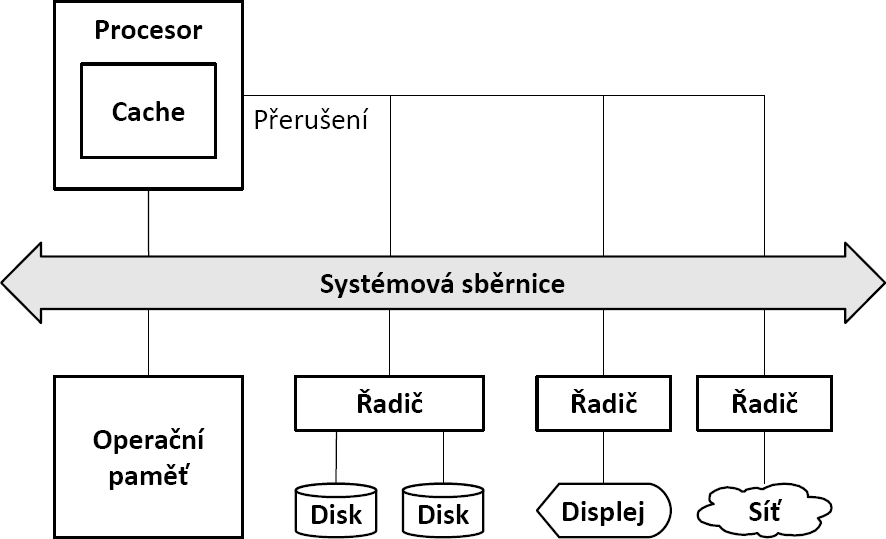
\includegraphics[width=8cm]{informatika/operacne_systemy_a_hw/obrazky/architektura.png}
  \end{center}

\textbf{Zpracov�n� instrukc�}
\begin{pitemize}
      \item \textbf{�ten�} instrukce z pam�ti na adrese v registru PC (program counter, obsahuje adresu n�sleduj�c� instrukce)
      \item \textbf{dek�dov�n�} instrukce a �ten� operand� z registr�
      \item \textbf{vykon�n�} operace odpov�daj�c� instruk�n�mu k�du (operace s obsahem registr�, v�po�et adresy a �ten�/z�pis do pam�ti, porovn�n� operand� pro podm�n�n� skok)
      \item \textbf{ulo�en�} v�sledku do registru (v�sledek operace s registry, data p�e�ten� z pam�ti)
      \item \textbf{posun} PC na n�sleduj�c� instrukci (n�sleduj�c� instrukce n�sleduje bezprost�edn� za pr�v� �tenou
instrukc�, pokud nen� �e�eno jinak - tzn. podm�n�n�/nepodm�n�n�
skok, v�jimka)       
  \end{pitemize} 

  \textbf{Typy instrukci (architektura MIPS):}
  \begin{pitemize}
      \item operace registr/registr, registr/immediate\footnote{operand (��slo) ulo�en�
      p��mo ve strojov�m k�du} (ALU operace, p�esun dat mezi registry)
      \item p�esuny dat registr/pam� (load/store architektura)
      \item podm�n�n� skoky (p�i rovnosti/nerovnosti obsahu dvou registr�)
      \item nepodm�n�n� skoky (v�etn� nep��m�ch skok� a skok� do podprogramu)
      \item speci�ln� instrukce (pr�ce se speci�ln�mi registry)
  \end{pitemize} 
\end{e}

\begin{e}{Start-up PC}{1}{zm��knu \uv{power on} a n�sleduje...}
\begin{penumerate}
    \item \emph{procesor} za�ne vykon�vat k�d (program) BIOSu (Basic Input/Output System)
    \item \emph{BIOS} zjist�, jak� HW je nainstalov�n, provede inicializaci grafick� karty a z (u�ivatelem definovan�ho) disku na�te a spust� boot sektor
    \item \emph{boot sektor} obsahuje k�d, kter� s pomoc� slu�eb BIOSu p�e�te z disku a spust� zavad�� OS
    \item \emph{zavad�� OS} p�e�te z disku k�d OS a spust� ho
    \item OS nastartuje syst�mov� slu�by a u�ivatelsk� rozhran�
\end{penumerate}
\end{e}

\begin{reportN}{Bulej}
Tenhle �lov�k se v tom vrtal hodn�, ale j� m�m tu v�hodu, �e jsem na st�edn� chodil na elektropr�myslovku, tak�e instrukc� a typ� instrukc� jsem mu tam popsal spoustu a i postup, jak procesor vykon�v� program, jsem v�d�l do detail� (a do detail� to cht�l). P�esv�d�il jsem ho asi hlavn� t�m, �e jsem odpov�dal takov�m t�m "samoz�ejm�m" zp�sobem ("a kdy� procesor vykon� instrukci, co d�l� d�l?" -"pokra�uje dal�� instrukc�" "no ale co p�esn� d�l�" -"no tenhle postup znovu, na�te dal�� instrukci..." "co to p�esn� znamen�?" -"no prost� zv�t�� instruction pointer o velikost pr�v� zpracovan� instrukce a t�m z�sk� adresu n�sleduj�c� instrukce, a opakuje tenhle postup").
\end{reportN}

\begin{reportN}{Peterka}
Peterka si narozdiel od Skopala aj precital to co som si napisal na papier. Popisal som tam Von Neumanna a Harvardsku architekturu (napisal som tam vsetko z vypiskov). K tomu nemal vyhrady. Potom vsak prisla horsia cast ked sa ma zacal vypytovat otazky typu: 

myslite si ze je dobre/zle ked moze byt prepisana ta pamat kde sa nachadza program, alebo ake su vyhody programovatelneho radica... dalej sa ma pytal na SISD,SIMD,MISD,MIMD, mal som mu nakreslit MISD ... co som moc nevedel... potom sa ma spytal na rozdiel Instruction flow control/Data flow control... dialog s Peterkom mi prisiel v niektorich castiach skor ako jeho monolog s mojim prikyvovanim hlavy...

Akorat jsem nebyl schopny si vzpomenout na architektury rizenou daty. A chtel vedet kolik radicu a ALU je potreba pri instrukcich SIMD,MIMD. Znamku nevim.

DATA FLOW + CONTROL FLOW (asi :)) podot�zka u mikroprocesor� a architektury 
\end{reportN}

\begin{reportN}{Peterka}
Von Neumannova architektura - dost temno
Harvardsk� Architektura - z�blesky
stroje ��zen� daty - brrr hr�za
tady u� ot�zky opravdu nev�m...
dod�m jen nepodce�te hardware - peterka d�v� v�dy jednu hardwarovou a jednu s�ovou ot�zku
dopl�uj�c�:
jak� jsou volac� konvence v Pascalu a C? viz zpracovan� ot�zky
co se stane kdy� zavol�me virtu�ln� fci p�ed vol�n�m konstruktoru? kone�n� jsem se chytil .)
\end{reportN}

\begin{reportN}{T�ma}
Za ferove povazujem ze vzal v uvahu ze som IOI a nedal mi konkretnu podotazku, skor tak prehladovo vsetko od architektur, cez procesory az po IO. Na druhej strane sa dost vrtal v zberniciach o ktorych som toho vedel pramalo ( myslim, ze v tych materialoch na statnice tam toho o nich moc nebolo ). Ked som zacal hovorit o preruseni, tak ma prerusil s tym, ze ak nechcem dopadnut ako kolega predo mnou ( patrne ho vyhodil ) tak nech som ticho
\end{reportN}

\subsection{Procesory, multiprocesory}

\begin{definiceN}{Procesor} 
Procesor (CPU – central processing unit) je ústřední výkonnou jednotkou počítače, která čte z paměti instrukce a na jejich základě vykonává program.

Základnými súčasťami procesora sú:
\begin{pitemize}
	\item řadič nebo řídicí jednotka, která řídí tok programu, tj. načítání instrukcí, jejich dekódování, načítání operandů instrukcí z operační paměti a ukládání výsledků zpracování instrukcí
	\item sada registrů k uchování operandů a mezivýsledků.
	\item jedna nebo více aritmeticko-logických jednotek (ALU), které provádí s daty aritmetické a logické operace.
	\item některé procesory obsahují jednu nebo několik jednotek plovoucí čárky (FPU), které provádí operace v plovoucí řádové čárce.
\end{pitemize}
\end{definiceN}

\begin{poznamka}
Súčasné procesory navyše často obsahujú ďalšie rozsiahle funkčné bloky (cache, rôzne periférie)~-- ktoré z \uv{ortodoxného hladiska} nie sú priamo súčasťou \emph{jadra procesoru}. Niektoré procesory môžu obsahovať viac jadier (+logiku slúžiacu k ich vzájomnému prepojeniu). Ďalším trendom je SoC (System on Chip), kde sa na čipe procesora nachádzajú aj ďalšie subsystémy napr. na spracovanie zvuku, grafiky alebo pripojenie externých periférií (takéto riešenia sa využívajú väčšinou v PDA, domácej elektronike, mobiloch atď.).
\end{poznamka}

\begin{obecne}{Dělení podle instruční sady}
Podľa inštrukčnej sady je možné procesory rozdeliť na:
\begin{pitemize}
	\item \textbf{CISC} (Complex Instruction Set Computer): poskytuje rozsiahlu inštrukčnú sadu spolu s rôznymi variantami inštrukcií. Jedna inštrukcia napr. môže vykonať veľa low-level operácií (načítanie z pamäti, vykonať aritmetickú operáciu a výsledok uložiť). Takéto inštrukcie zjednodušovali zápis programov (inštrukcie boli bližšie vyšším programovacím jazykom) a zmenšovali veľkosť programu a počet prístupov do pamäti~-- čo bolo v 60tych rokoch dôležité. Avšak nie vždy je vykonanie jednej zložitej operácie rýchlejšie ako vykonanie viac menej zložitých miesto toho (napr. kvôli zložitému dekódovaniu a použitiu mikrokódu na volanie jednoduchých \uv{podinštrukcií}). Príkladmi CISC architektúr procesorov sú System/360, Motorola 68000 a Intel x86. V súčasnosti napr. x86 rozkladá zložité inštrukcie na \uv{micro-operations} ktoré môžu byť pipeline-ou spracované paralelne a vyšší výkon je tak dosahovaný na väčšom rozsahu inštrukcií. Vďaka tomu sú súčasné x86 procesory minimálne rovnako výkonné ako ozajstné RISC architektúry.
	\item \textbf{RISC} (Reduced Instruction Set Computer): design CPU ktorý uprednosňuje jednoduchšiu inštrukčnú sadu a menšiu zložitosť adresovacích modelov~-- vďaka čomu je možné dosiahnuť lacnejšiu implementáciu, väčšiu úroveň paralelizmu a účinnejšie kompilátory. Dôvodom vzniku bolo aj nevyužívanie celej CISC inštrukčnej sady a upredňostňovania len obmedzenej podmnožiny (designéri procesorov potom optimalizovali len tieto podmnožiny a tak sa zvyšné inštrukcie používali ešte menej...). Kvôli väčšiemu počtu inštrukcií však musia RISC procesory častejšie pristupovať k pamäti... Príkladmi RISC procesorov sú napr. SPARC a ARM. V architekturách typu \textbf{Post-RISC} jde o spojení RISCových vlastností s technikami zvýšení výkonu, jako je out-of-order vykonávání a paralelismus.
    \item \textbf{VLIW}: Very Long Instruction Word or VLIW refers to a CPU architecture designed to take advantage of instruction level parallelism (ILP). A processor that executes every instruction one after the other (i.e. a non-pipelined scalar architecture) may use processor resources inefficiently, potentially leading to poor performance. The performance can be improved by executing different sub-steps of sequential instructions simultaneously (this is pipelining), or even executing multiple instructions entirely simultaneously as in superscalar architectures. The VLIW approach, on the other hand, executes operation in parallel based on a fixed schedule determined when programs are compiled. Since determining the order of execution of operations (including which operations can execute simultaneously) is handled by the compiler, the processor does not need the scheduling hardware that the three techniques described above require. As a result, VLIW CPUs offer significant computational power with less hardware complexity (but greater compiler complexity) than is associated with most superscalar CPUs.
    \item \textbf{EPIC}: (Někdy označován za poddruh VLIW) Explicitly Parallel Instruction Computing (EPIC) is a computing paradigm that began to be researched in the 1990s. This paradigm is also called Independence architectures. It was used by Intel and HP in the development of Intel’s IA-64 architecture, and has been implemented in Intel’s Itanium and Itanium 2 line of server processors. The goal of EPIC was to increase the ability of microprocessors to execute software instructions in parallel, by using the compiler, rather than complex on-die circuitry, to identify and leverage opportunities for parallel execution. This would allow performance to be scaled more rapidly in future processor designs, without resorting to ever-higher clock frequencies, which have since become problematic due to associated power and cooling issues.
\end{pitemize}
\medskip
TODO: asi opravit, možná zpřesnit VLIW a EPIC a určitě přeložit

\medskip
Řekneme, že procesor má \emph{ortogonální instrukční sadu}, pokud žádná instrukce nepředpokládá implicitně použití některých registrů. To umožňuje jednodušší práci algoritmům přidělování registrů v překladačích. Příkladem neortogonální instrukční sady je i x86.
\end{obecne}

\begin{obecne}{Další dělení}
Ďalej je možné procesory rozdeliť podľa dĺžky operandov v bitoch (8, 16, 32, 64...), ktorý je procesor schopný spracovať v jednom kroku. V embedded zariadeniach sa najčastejšie používajú 4- a 8-bitové procesory. V PDA, mobiloch a videohrách 8 resp. 16 bitové. 32 a viac bitov využíajú napr. osobné počítače a laserové tlačiarne.

Dôležitou vlastnosťou je aj taktovacia frekvencia jadra, MIPS (millions of instructions per second) a jeho rýchlosť. V súčasnosti je ťažké dávať do súvislosti výkon procesorov s ich frekvenciou (resp. MIPS)~-- kým Pentium zvládne na výpočet vo floatoch, jednoduchý 8-bitový PIC na to potrebuje oveľa viac taktov. Ďalším \uv{problémom} je superskalarita procesorov, ktorá im umožňuje vykonať viacero nezávislých inštrukcií počas jedného taktu.
\end{obecne}

\begin{obecne}{Techniky pro zvýšení výkonu}
Zvyšovať výkon (procesorov) je možné viacerými spôsobmi. Najjednoduchším (a najpomalším) typom je Subskalárny CPU (načíta a spracúva len jednu inštrukciu naraz~-- preto musí celý procesor čakať kým vykonávanie inštrukcie skončí; je tak zdržovaný dlhšie trvajúcimi inštrukciami). 

\begin{center}
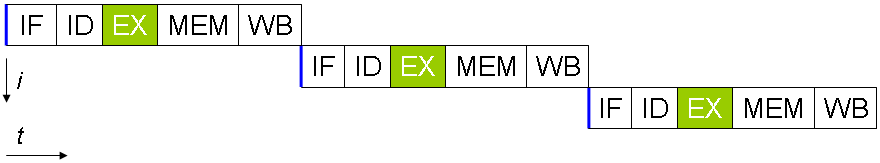
\includegraphics[width=8cm]{informatika/operacne_systemy_a_hw/obrazky/Nopipeline.png}
\end{center}

Pokusy o dosiahnutie skalárneho a lepšieho výkonu vyústili do designov ktoré sa správajú menej lineárne a viac paralelne. Čo sa týka paralelizmu v procesoroch, používajú sa dva druhy pojmov na ich klasifikáciu~-- \emph{Instruction level parallelism} (zvyšovanie rýchlosti vykonávania inštrukcií v procesore a teda zväčšovanie využitia prostriedkov na čipe) a \emph{Thread level parallelism} (zväčšovanie počtu vlákien, ktoré dokáže CPU vykonávať naraz).
\begin{pitemize}
  \item \textbf{pipeline}: 
  Zlepšenie je možné dosiahnúť pomocou \uv{instruction pipelining}-u, ktoré je použíté vo väčšine moderných procesorov. Umožňuje vykonanie viac ako jednej inštrukcie v jednom kroku vďaka rozloženiu spracovávania inštrukcie na viac menších krokov: 
  \begin{center}
  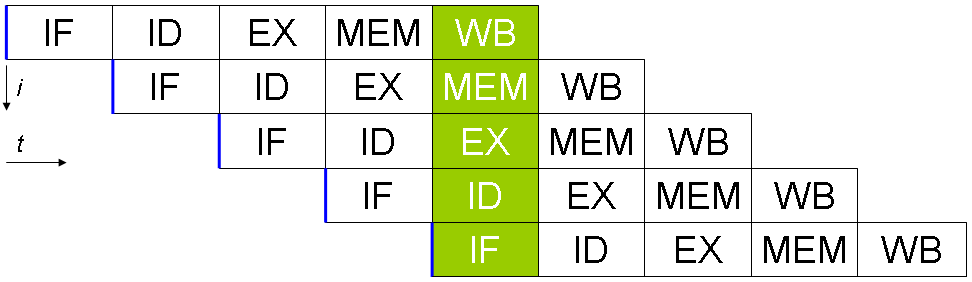
\includegraphics[width=8cm]{informatika/operacne_systemy_a_hw/obrazky/Fivestagespipeline.png}
  \end{center}

  \item \textbf{superskalarita}: Dialša možnosť je použitie superscalar designu, ktorý obsahuje dlhú inštrukčnú pipeline a viacero identických execution jednotiek.  
  \begin{center}
  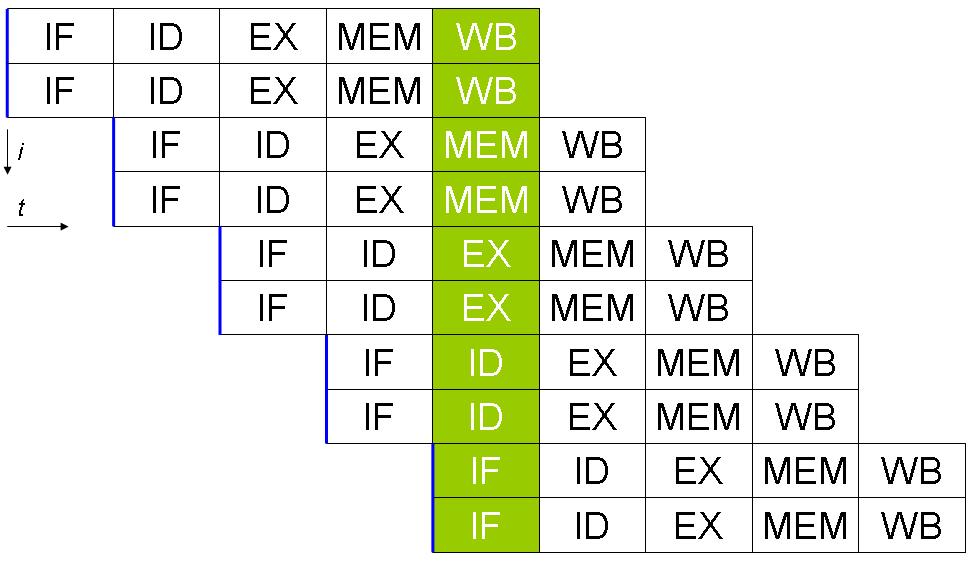
\includegraphics[width=8cm]{informatika/operacne_systemy_a_hw/obrazky/Superscalarpipeline.png}
  \end{center}	

  \item \textbf{Out of order execution}
  \begin{penumerate}
	  \item Načtení instrukce, případně její rozdrobení na mikroinstrukce
	  \item Zařazení do vyčkávací stanice (instruction pool)
	  \item Instrukce čeká na všechny svoje operandy
	  \item Instrukce se vykoná ve své výkonné jednotce (je vybírána z instruction poolu nezávisle na ostatních)
	  \item Výsledky se uchovají ve frontě (reorder buffer)
	  \item Až se všechny starší instrukce zapíší do registrů, zapíše se výsledek této instrukce (opětovné řazení)
  \end{penumerate}

  \item \textbf{Predikce skoků}~-- hluboké pipeliny mají problém, pokud podmíněný skok není proveden; dynamická predicke skoků (historie CPU~-- vzory nějaké hloubky) vs. statická (bez nápovědy~-- skok vpřed se neprovede, skok vzad se provede; s nápovědou~-- překladač odhaduje pravděpodobnost skoku)

  \item \textbf{Spekulativní vykonávaní}~-- vykonávání kódu, který nemusí být zapotřebí; významná disproporce mezi rychlostí CPU a paměti; typické využití je značné předsunutí čtecích operací; CPU provádí i odsouvání zápisových operací


  \item \textbf{Data parallelism}: SIMD inštrukcie (napr. multimediálne inštrukcie), vektorové procesory...
\end{pitemize}
\end{obecne}

\subsubsection*{Multiprocesory}

TODO: jde o copy \& paste z Wiki ... předělat česky/slovensky
\medskip

\begin{definiceN}{Multiprocesor}
  O \emph{multiprocesoru} mluvíme, pokud je použito dvou nebo více procesorů
  (CPU) v rámci jednoho počítačového systému. Termín je také používán mluvíme-li
  o schopnosti systému využívat více procesorů a/nebo schopnosti rozdělovat
  úlohy mezi jednotlivými procesory.
\end{definiceN}

\begin{obecne}{Vztah k datům a instrukcím}
In multiprocessing, the processors can be used to execute a single sequence of instructions in multiple contexts (single-instruction, multiple-data or SIMD, often used in vector processing), multiple sequences of instructions in a single context (multiple-instruction, single-data or MISD, used for redundancy in fail-safe systems and sometimes applied to describe pipelined processors or hyperthreading), or multiple sequences of instructions in multiple contexts (multiple-instruction, multiple-data or MIMD).
\end{obecne}

\begin{obecne}{Symetrie}
In a multiprocessing system, all CPUs may be equal, or some may be reserved for special purposes. A combination of hardware and operating-system software design considerations determine the symmetry (or lack thereof) in a given system. For example, hardware or software considerations may require that only one CPU respond to all hardware interrupts, whereas all other work in the system may be distributed equally among CPUs; or execution of kernel-mode code may be restricted to only one processor (either a specific processor, or only one processor at a time), whereas user-mode code may be executed in any combination of processors. Multiprocessing systems are often easier to design if such restrictions are imposed, but they tend to be less efficient than systems in which all CPUs are utilized equally.

Systems that treat all CPUs equally are called symmetric multiprocessing (SMP) systems. In systems where all CPUs are not equal, system resources may be divided in a number of ways, including asymmetric multiprocessing (ASMP), non-uniform memory access (NUMA) multiprocessing, and clustered multiprocessing (qq.v.).
\end{obecne}

\begin{obecne}{Těsnost spojení multiprocesorů}
\begin{pitemize}
    \item \textbf{Tightly-coupled} multiprocessor systems contain multiple CPUs that are connected at the bus level. These CPUs may have access to a central shared memory (SMP or UMA), or may participate in a memory hierarchy with both local and shared memory (NUMA). The IBM p690 Regatta is an example of a high end SMP system. Intel Xeon processors dominated the multiprocessor market for business PCs and were the only x86 option till the release of AMD's Opteron range of processors in 2004. Both ranges of processors had their own onboard cache but provided access to shared memory; the Xeon processors via a common pipe and the Opteron processors via independent pathways to the system RAM.

    \item \textbf{Chip multiprocessors}, also known as multi-core computing, involves more than one processor placed on a single chip and can be thought of the most extreme form of tightly-coupled multiprocessing. Mainframe systems with multiple processors are often tightly-coupled.

    \item \textbf{Loosely-coupled multiprocessor} systems (often referred to as clusters) are based on multiple standalone single or dual processor commodity computers interconnected via a high speed communication system (Gigabit Ethernet is common). A Linux Beowulf cluster is an example of a loosely-coupled system.
\end{pitemize}
Tightly-coupled systems perform better and are physically smaller than loosely-coupled systems, but have historically required greater initial investments and may depreciate rapidly; nodes in a loosely-coupled system are usually inexpensive commodity computers and can be recycled as independent machines upon retirement from the cluster.

\textbf{SMP} (Symmetric Multiprocessing): viac procesorov so zdieľanou operačnou pamäťou (nutné mechanizmy na zabránenie nesprávnych náhľadov na pamäť a migráciu procesov medzi procesormi). SMP systems allow any processor to work on any task no matter where the data for that task are located in memory; with proper operating system support, SMP systems can easily move tasks between processors to balance the workload efficiently.
\end{obecne}

\subsection{Sb�rnice, protokoly}

\begin{pitemize}
	\item \textbf{Struktura sb�rnice}: datov� linky, adresov� linky, ��d�c� linky
	\item \textbf{Synchronn� p�enos} (vznik ud�losti je d�n hodinov�m sign�lem) vs. \textbf{asynchronn� p�enos} (vznik ud�losti je ur�en p�edch�zej�c� ud�lost�~-- napr. signaliz�ciou za�iatku d�t) 
	\item \textbf{Parametry sb�rnice}: 
	\begin{pitemize}
	  \item \emph{datov� ���ka}~-- po�et p�en�en�ch bit� v jednom okam�iku,
	  \item \emph{kapacita}~-- po�et bit� p�enesen�ch za �as,
	  \item \emph{rychlost}~-- kapacita sb�rnice normovan� k jednotce informace. 
	\end{pitemize}  
	\item \textbf{��zen� po�adavk�}: 
	\begin{pitemize}
	  \item \emph{centr�ln�}~-- n�hodn�, dle po�ad� vzniku po�adavk�, prioritn�,
	  \item \emph{distribuovan�}~-- kolizn� (CSMA/CD), token bus, prioritn� linka (daisy chain).
	\end{pitemize} 
	\item \textbf{P�enos dat po sb�rnici} m��e prob�hat bu� za ��asti procesoru (zdroj $\rightarrow$ CPU $\rightarrow$ c�l), nebo bez. Bez procesoru to m��e b�t nap�.:
	\begin{pitemize}
		\item d�vkov� re�im~-- domluva mezi CPU a �adi�em na dob� obsazen� sb�rnice (napr. pomocou zdvihnutia \uv{lock flagu} na zbernici)
		\item kraden� cykl�~-- �adi� na dobu p�enosu \uv{usp�} procesor (nelze uspat na dlouho, je to technicky n�ro�n�j��)
		\item transparentn� re�im~-- �adi� rozezn�, kdy procesor nepou��v� sb�rnici, obvykle nelze v�t�� p�enosy najednou
		\item DMA (Direct Memory Access)~-- speci�ln� jednotka pro prov�d�n� p�enos� dat (mezi za��zen�mi a pam�t�)
	\end{pitemize}
	Jednou z technik, pou��van�ch k p�enosu dat po sb�rnici �adi�i DMA, je \emph{scatter-gather}. Znamen� to, �e v r�mci jednoho p�enosu se zpracov�v� v�c ne nutn� souvisl�ch blok� dat. 
	\begin{pitemize}
	    \item \emph{scatter}~-- DMA �adi� v r�mci 1 p�enosu ulo�� z 1 m�sta data na n�kolik r�zn�ch m�st (nap� hlavi�ky TCP/IP - jinak zbyte�n� kop�rov�n�)  
	    \item \emph{gather}~-- nap�. p�i str�nkov�n� pam�ti - na��t�n� str�nek, kter� fyzicky na disku nemus� b�t u sebe, slo�en� na 1 m�sto do pam�ti.
	\end{pitemize}
\end{pitemize}

P��klady sb�rnic:
\begin{pitemize}
	\item ISA, EISA
	\item ATA, ATAPI~-- UltraDMA, Serial-ATA (SATA)
	\item SCSI (Small Computer System Interface)
	\item PCI, PCI-X, PCI Express
	\item AGP (Advanced Graphics Port)
	\item USB (Universal Serial Bus)
	\item FireWire (IEEE 1394)
	\item RS485
	\item $I^{2}C$
\end{pitemize}

P��buzn� sb�rnic:
\begin{pitemize}
	\item IrDA
	\item Bluetooth
	\item Wi-Fi, WiMAX 
\end{pitemize}

\subsection{Vstupn� a v�stupn� za��zen�, ukl�d�n� a p�enos dat}

Za��zen� maj� r�zn� charakteristiky:
\begin{pitemize}
    \item \textbf{druh}~-- blokov� (disk, s�ov� karta), znakov� (kl�vesnice, my�)
    \item \textbf{p��stup}~-- sekven�n� (datov� p�ska), n�hodn� (hdd, cd)
    \item \textbf{komunikace}~-- synchronn� (pracuje s daty na ��dost~-- disk), asynchronn� (\uv{nevy��dan�} data~-- s�ov� karta)
    \item \textbf{sd�len�}~-- sd�len� (preemptivn�, lze odebrat~-- s�ov� karta (po multiplexu OS)), vyhrazen� (nepreemptivn�~-- tisk�rna, sd�len� se realizuje p�es \textbf{spooling} - frontou). Re�ln� se rozd�ly st�raj�.
    \item \textbf{rychlost} (od n�kolika Bps po GBps)
    \item \textbf{sm�r dat}~-- R/W, R/O (CD-ROM), W/O (tisk�rna) 
\end{pitemize}

\begin{e}{Propojovac� syst�my}{0}{0}
D�l� se na \textbf{dvoubodov� spoje} (vztah 1:1), jde nap�. o p��m� spojen� porty, k��ov� p�ep�na�, kde nen� nutn� ��dn� adresace. Druhou mo�nost� jsou \textbf{v�cebodov� spoje}, kde v�ce ��astn�k� sd�l� p�enosov� m�dium jako nap�. sb�rnice nebo p�i broadcastingu.
\end{e}

\textbf{Procesor} m��e p�istupovat k I/O za��zen�m dv�ma zp�soby:
\begin{pitemize}
    \item \textbf{port-mapped I/O} -- speci�ln� adresov� port CPU, kter� m� i speci�ln� instrukce pro pr�ci (IN, OUT) s I/O za��zen�m, kter� tak� maj� vlastn� adresov� prostor (bu� p��mo vlastn� sb�rnici, nebo extra I/O pinem), d�ky tomu se tak� ��k� \uv{isolated I/O},
    \item \textbf{memory-mapped I/O} -- pam�ov� mapov�n�, kter� mapuje I/O za��zen� p��mo do adresov�ho prostoru fyzick� pam�ti. Tato ��st adresov�ho prostoru m��e b�t vyhrazen� trvale nebo i jen do�asn�. Za��zen� poslouch� na adresov� sb�rnici, aby v�d�lo, kdy m� pracovat (odpov�dat, ...).
\end{pitemize}

  \begin{center}
    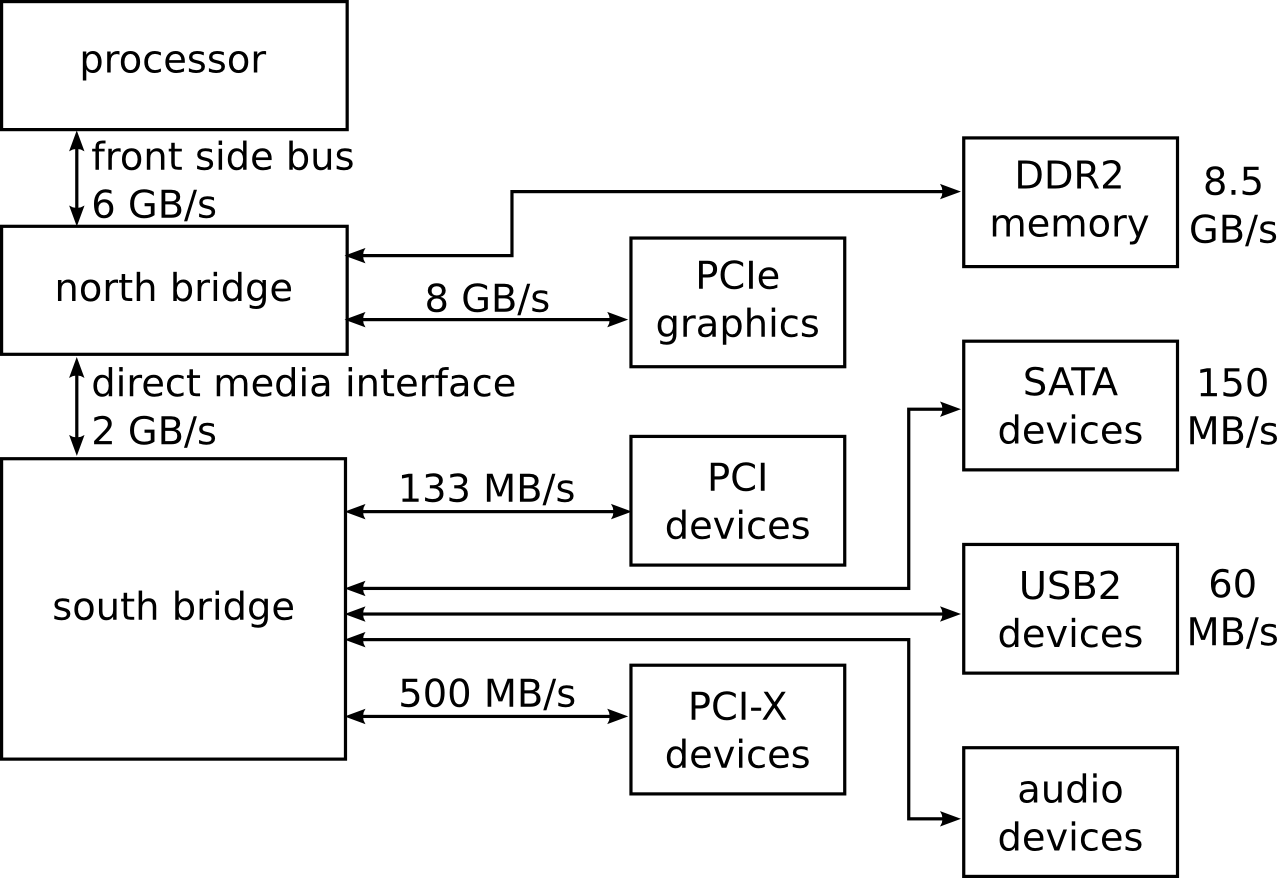
\includegraphics[width=8cm]{informatika/operacne_systemy_a_hw/obrazky/bus_north_south_bridge.png}
  \end{center}

\begin{e}{Sb�rnice}{0}{0}
Sb�rnice je sada vodi�� propojuj�c� v�ce za��zen�. Vodi�e jsou odd�len� pro ��zen� (po�adavky, potvrzen�, typ dat) a data (p�enos dat, adresov�n�). V�hodou je univerz�lnost a n�zk� cena, nev�hodami pak omezen� d�lkou a dan� v d�sledku pou��v�n� rozmanit�ch za��zen�, tak� potenci�ln� \uv{bottleneck}.\\
Transakce na sb�rnici za��n� po�adavkem (vysl�n� p��kazu a adresy c�le), na kter� mus� c�l odpov�d�t potvrzen�m, na�e� n�sleduje p�enos dat mezi ��astn�ky \textbf{master/initiator} (kte�� pos�laj� po�adavek) a \textbf{slave/target}, kte�� pos�laj�/p�ij�maj� data.\\
\textbf{��zen�} -- \textbf{synchronn�} (podle hodin, jednodu���, rychlej��, ale omezen� d�lka sb�rnice a stejn� �as v�em) vs. \textbf{asynchronn�} (obecn�j��, slo�it�j��, zato bez omezen� d�lky, ale s ni��� rychlost�, nap�. USB, FireWire)\\
\textbf{p�id�lov�n�} -- \textbf{centralizovan�} (master ��d� a �ek� na p�id�len�, kter� p�id�luje arbitr podle priority a fairness, master po proveden� operace d� arbitrovi v�d�t, �e je sb�rnice op�t voln�) vs. \textbf{distribuovan�}, kter� m��e b�t kolizn� nebo zalo�en� na \uv{samov�b�ru}.
\end{e}

\begin{figure}[h]
  \centering
  \subfloat[polling]{\label{fig:bus_polling}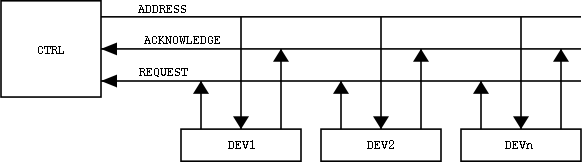
\includegraphics[width=0.49\textwidth]{informatika/operacne_systemy_a_hw/obrazky/bus_polling.png}} \hfill
  \subfloat[prioritn� z�et�zen�, daisy chain]{\label{fig:bus_daisy_chain}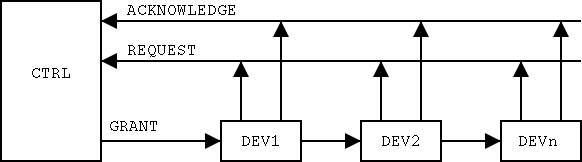
\includegraphics[width=0.49\textwidth]{informatika/operacne_systemy_a_hw/obrazky/bus_daisy_chain.png}} \hfill
  \subfloat[nez�visl� ��dosti]{\label{fig:bus_independent}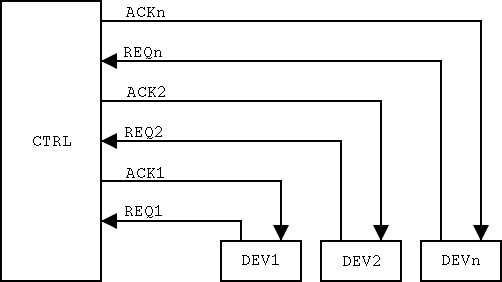
\includegraphics[width=7cm]{informatika/operacne_systemy_a_hw/obrazky/bus_independent.png}}
    \caption{centralizovan� p�id�lov�n�}
  \label{fig:bus_centralizovane_pridelovani}
\end{figure}
Informace o stavu za��zen� m��e CPU z�sk�vat:
\begin{pitemize}
    \item \textbf{polling}~-- aktivn� �ek�n� na zm�nu za��zen� (program periodicky kontroluje stav), pro pomal� za��zen� vznik� zna�n� re�ie
    \item \textbf{interrupt-driven I/O}~-- asynchronn� p�eru�en� od za��zen�, kter� samo signalizuje zm�nu stavu, na co� reaguje obslu�n� rutina. CPU ov�em nen� na p�eru�en� p�ipraven, tak mus� ulo�it stav programu $\rightarrow$ stoj� to �as. CPU mus� podporovat tuto signalizaci p�eru�en�, identifikovat zdroj p�eru�en�, vybrat spr�vnou obslu�nou rutinu. Syst�m mus� zajistit doru�en� p�eru�en� k CPU a d�le �adi� jejich podle priority ur�� jejich po�ad� (m��e jich b�t v�ce ne� m� CPU vstup�). Pr�b�h:
    \begin{penumerate}
    \item     Vn�j�� za��zen� vyvol� po�adavek o p�eru�en�
    \item			I/O rozhran� vy�le sign�l IRQ na �adi� p�eru�en� (na port IRQ 2)
    \item     �adi� p�eru�en� vygeneruje sign�l INTR � �n�kdo� ��d� o p�eru�en� a vy�le ho k procesoru.
    \item     Procesor se na z�klad� maskov�n� rozhodne obslou�it p�eru�en� a sign�lem INTA se zept�, jak� za��zen� ��d� o p�eru�en�.
    \item     �adi� p�eru�en� identifikuje za��zen�, kter� ��d� o p�eru�en� a ode�le ��slo typu p�eru�en� k procesoru
    \item     Procesor ulo�� stavov� informace o pr�v� zpracov�van�m programu do z�sobn�ku.
    \item     Podle ��sla typu p��choz�ho p�eru�en� nalezne ve vektoru p�eru�en� adresu p��slu�n�ho obslu�n�ho podprogramu.
    \item     Vyhled� obslu�n� podprogram obsluhy p�eru�en� v pam�ti a vykon� ho.
    \item     Po proveden� obslu�n�ho programu op�t obnov� ulo�en� stavov� informace ze z�sobn�ku a p�eru�en� program pokra�uje d�l.
\end{penumerate}
    
\end{pitemize}

P�enos dat mezi za��zen�m a CPU/pam�t�:
\begin{penumerate}
    \item \textbf{PIO (Programmed I/O)}~-- data p�en�ena za ��asti CPU (pln� zam�stn�n), p�enos realizov�n cyklem v programu, rychl� p�enos, ale neefektivn� vyu�it� CPU, pak p�i�lo DMA
    \item \textbf{DMA (Direct Memory Access)}~-- za��zen� si samo ��d� p��stup na sb�rnici a p�en�� data z/do pam�ti bez ��asti CPU; po skon�en� p�enosu p�eru�en� (ozn�men� o dokon�en�) nap�, p�enos dat mezi HDD a RAM
\end{penumerate}

\begin{e}{Bus mastering}{0}{0}
Slou�� pro p�enos dat mezi za��zen�m a pam�t� nebo mezi dv�ma za��zen�mi. Jde o to, �e sb�rnici m��e ��dit (za��t transakci, b�t masterem) libovoln� ��astn�k (CPU vn�m�n jako jeden z nich), st�le je nutn� p�enos \emph{nastavit} z programu.
\end{e}

\subsubsection*{DMA}
CPU nastav� p�enos a nech� DMA pracovat, a� je operace dokon�ena, po�le se p�eru�en�, tedy mezit�m m��e CPU pracovat jinde. DMA �adi� je obvod pro ��zen� p�enos� na sb�rnici mezi pam�t� a za��zen�mi nebo i pouze v pam�ti. U multiprocesor� se u��v� i k p�enosu dat mezi j�dry. D�le b�n� u pevn�ch disk�, grafick�ch, zvukov�ch a s�ov�ch karet. DMA �adi� obsahuje registry, do kter�ch m��e CPU zapisovat nastaven� p�enosu (adresa v pam�ti, po�et byt�, sm�r r/w, jak� za��zen�) -- tomu se ��k� \textbf{burst mode}, ve kter�m vysta�� jeden adresov� cyklus na cel� blok dat. D�le se vyu��v� p�i p�enosu dat do/z v�ce nesouvisl�ch buffer� (\textbf{scatter/gather}, tak� vektorov� I/O).

\begin{e}{Pr�ce �adi�e DMA}{0}{0}
\begin{pitemize}
    \item generuje adresy pam�ti a periferie, generuje ��d�c� sign�ly pro �ten�/z�pis
    \item generuje sign�ly pro procesor, aby zajistil, �e procesor nep�istupuje (nezapisuje) na sb�rnici
    \item �adi� s�m se chov� jako periferie
    \item program nastavuje parametry p�enosu, tj. odkud se bude p�en�et, kam, a kolik (2 ��ta�e, kan�l DMA)
    \item za��zen� p�ipojena na kan�l DMA, p�i p�enosu je c�lov� za��zen� aktivov�no �adi�em, nikoliv vystaven�m adresy   
\end{pitemize}
\end{e}

\begin{e}{Posloupnost ud�lost�}{0}{0}
��sla p�ed ud�lost� odpov�daj� ��sl�m na obr�zku n�e.
\begin{pitemize}
    \item program nastav� �adi� a periferii a povol� p�enos
    \item[(1)] aktivac� sign�lu DREQx periferie po��d� �adi� DMA o p�enos slova z/do pam�ti
    \item �adi� DMA zkontroluje nastaven� kan�lu vyhodnot� prioritu ��dosti
    \item[(2)] aktivac� sign�lu HOLD �adi� DMA po��d� CPU o p�id�len� sb�rnice
    \item[(3)] pokud CPU nepot�ebuje sb�rnici, odpoj� se od sb�rnice a signalizuje HLDA
      \subitem - CPU po��d testuje HOLD na za��tku strojov�ho cyklu
    \item[(4)] po p�ijet� HLDA �adi� p�iprav� sb�rnici pro p�enos
    \subitem - vystav� adresu v pam�ti a ��d�c� sign�ly pro �ten�/z�pis z/do pam�ti/periferie
    \item[(5)] �adi� DMA aktivuje sign�l DACKx, kter�m vyzve periferii k vystaven�/p�e�ten� dat na/ze sb�rnice
    \item[(7)] v z�vislosti na re�imu bu� p�enos kon��, nebo pokra�uje dal��m slovem dokud je DREQx aktivn�
    \item p�i posledn�m slov� �adi� aktivuje sign�l EOP
    \item[(8)] p�i ukon�en� p�enosu �adi� uvoln� sign�l HOLD
    \item[(9)] procesor uvoln� HLDA a p�ipoj� se ke sb�rnici
\end{pitemize}
\begin{figure}[h]
  \centering
  \label{fig:dma_block_transfer}
  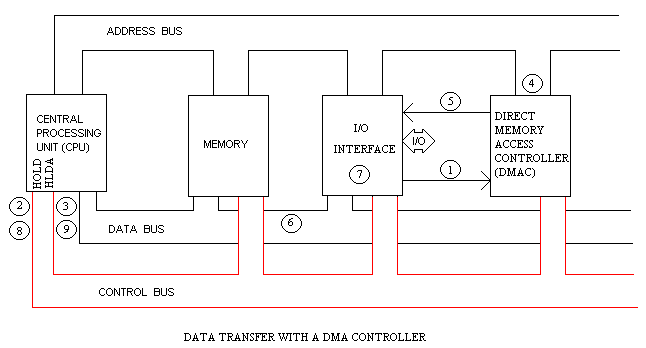
\includegraphics[width=17cm]{informatika/operacne_systemy_a_hw/obrazky/dma_block_transfer.png}
%  \caption{DMA burst mode}
\end{figure}
\end{e}

Probl�my u DMA spo��vaj� v odst�n�n� CPU od pam�ti, co� m��e vyvolat \textbf{pam�ovou koherenci}, slu�n� �e�eno pomoc� DMA obejdeme cache CPU, kde mohou b�t aktu�ln�j�� hodnoty ne� v pam�ti, a tud� m�me probl�m Houstone. �e�� se to t�m, �e procesor sleduje, na jak� adresy se p�istupuje a pokud tam padne n�jak�, kterou m� v cache, tak to za�ne �e�it.

\begin{figure}[h]
  \centering
  \label{fig:dma_memory_incoherency}
  
\includegraphics[width=12cm]{informatika/operacne_systemy_a_hw/obrazky/pametova_koherence.png}
  \caption{pam�ov� koherence}
\end{figure}

C�le I/O software:
\begin{pitemize}
    \item \textbf{Nez�vislost za��zen�}~-- programy nemus� dop�edu v�d�t, s jak�m p�esn� za��zen�m budou pracovat~-- je jedno jestli pracuji se souborem na pevn�m disku, disket� nebo na CD-ROM
    \item \textbf{Jednotn� pojmenov�n�} (na UNIXu /dev)
    \item \textbf{P�ipojen� (mount)}~-- �ast� u vym�niteln�ch za��zen� (disketa); mo�n� i u pevn�ch za��zen� (disk); nutn� pro spr�vnou funkci cache OS
    \item \textbf{Obsluha chyb}~-- v mnoha p��padech oprava bez v�dom� u�ivatele (velmi �asto zp�sobeno pr�v� u�ivatelem)
\end{pitemize}

\begin{reportN}{Bulej + Yaghob}
zapisal som vyse strany, ale to co ma yaghob na slidoch a to co je vo vypracovanom ucebnom texte ich ani trochu nezaujimalo. zaujimal ich popis DMA a preruseni, pricom sa pytali ako to presne funguje - chceli popisat instrukcie ako to moze prebiehat, ako sa to presne implementuje apod., co som bohuzial vobec nevedel
\end{reportN}

\begin{reportN}{Bulej} Prenos dat z disku do operacni pameti. P�ekvapiv� dobr� v�sledek, nicm�n� den p�edt�m jsem si �etl o DMA, tak�e bych to m�l v�d�t �ejo :-) Cht�l by prej je�t� v�d�t, �e to, co sed� na sb�rnici a ��d� ten p�enos, se ovl�d� z procesoru tak, �e v tom jsou n�jak� registry, do kterejch se hod� instrukce, a taky �e se na�tou data z disku do diskov� cache, pak se vyvol� p�eru�en�, a pak se teprva ty data n�jak dostanou do RAMky, t�ebas tim DMA nebo jinejma zp�sobama (a jakejma, pochopiteln�).
\end{reportN}

\subsection{Architektury OS}

\begin{obecne}{Klasick� struktura~-- monolitick�}
Nejstar��, u� IBM 360, Unix, Windown 95-ME, v�echny slu�by uvnit�, prov�d�ny ve chr�n�n�m m�du, j�dro pom�rn� velk�, \uv{�dajn�} nejrychlej��. Program zavol� slu�bu OS, p�es tabulku se zjist� adresa p��sl. fce, ta se zavol� a vr�t� v�sledek.  Nev�hoda: hor�� �dr�ba -- je-li v programu chyba, m��e po�kodit zb�vaj�c� ��sti syst�mu, roz�i�ov�n� za b�hu je komplikovan�. 
\end{obecne}

\begin{obecne}{Virtu�ln� stroje}
P�vodn� n�pad : Virtual Machine pro IBM360 -- odd�lit multitasking od OS jako ext. stroj. Nad HW byla dal�� vrstva -- \uv{Virtual Machine} -- m�la pl�novat, vyr�b� pro procesy iluzi hol�ho HW; dneska nap�. VMWare d�l� to sam�. Pro IBM360 se dalo pou��t v kombinaci s CMS (jedno�lohov�) i p�vodn�ho OS360 (rychlej�� ne� OS360 na hol�m HW). 

Dnes: definuji abstraktn� stroj, pro n�j p�ekl�d�m programy (.NET, Java) $\rightarrow$ p�enositelnost, kompatibilita (IBM AS400~-- des�tky let), probl�m~-- pomal�. 
\end{obecne}

\begin{obecne}{Mikroj�dro}
snaha aby ��st b��c� v kernel m�du byla co nejmen�� (t�eba jen cca 10 KB), nejnov�j��, experiment�ln�, �asto pro Distribuovan� OS (dnes u� nepou��van�), hodn� proces� \& komunikace (klient/server), mikroj�dro �e�� jenom komunikaci. 

Filesyst�m apod. jsou procesy -- aplikace jim pos�laj� p�es j�dro po�adavky.

v�hoda: kdy� n�co spadne, nepo�kod� to zbytek, moduly jdou m�nit za b�hu, komunikace jde snadno roz���it na komunikaci po s�ti. Pou��vaj� ho: Chorus (�st�edny), QNX a Symbian OS.
\end{obecne}

  \begin{center}
    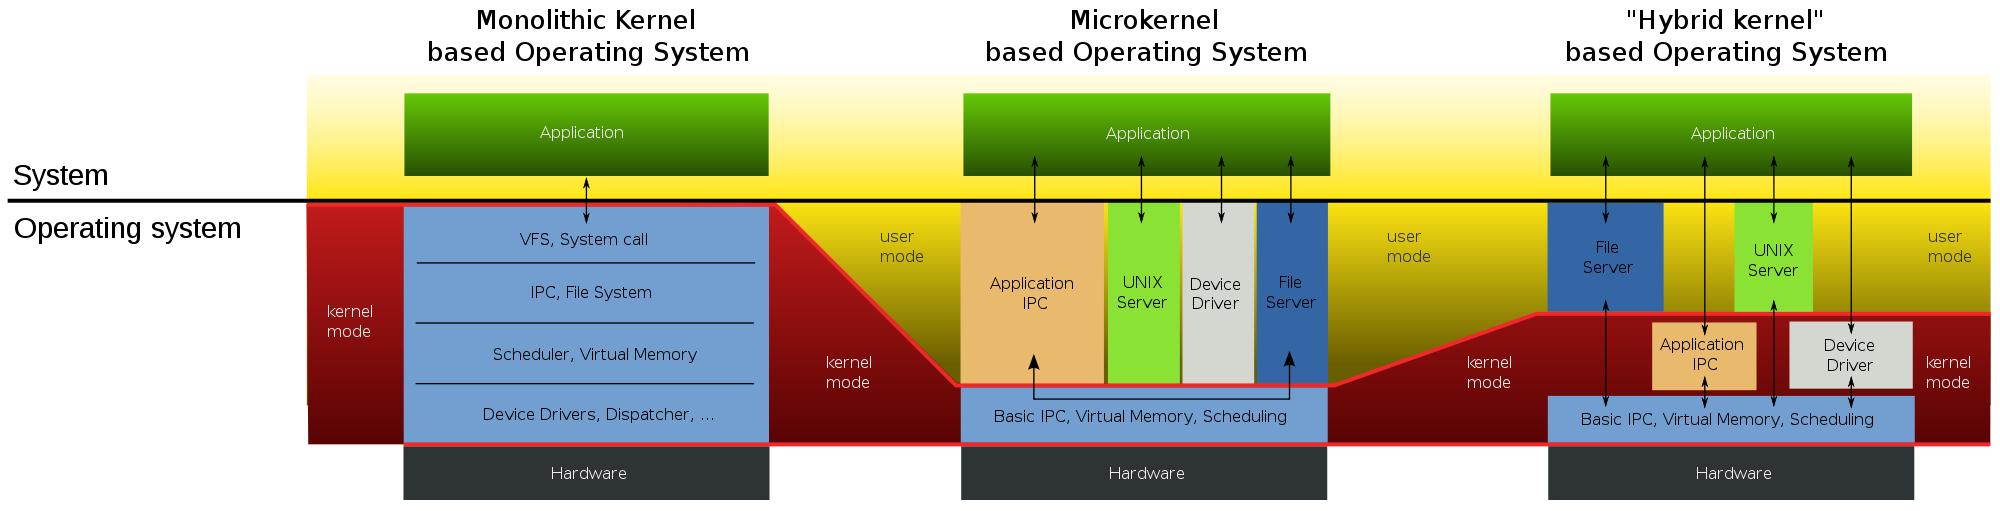
\includegraphics[width=19cm]{informatika/operacne_systemy_a_hw/obrazky/kernel.png}
  \end{center}

\begin{obecne}{Architektura WinNT}
  J�dro je pom�rn� mal� (cca 1MB), schopn� (pro vy��� vrstvy jsou n�kter� schopnosti skryt� - \textit{hybridn� j�dro}), na jeho vzniku se pod�leli schopn� Unix��i. Byla zde snaha o malou velikost, p�enositelnost. J�dro je neutr�ln� vzhledem k vy���m vrstv�m, nad n�m lze vybudovat r�zn� syst�my (Windows subsyst�m, POSIX, OS/2).

  Rozhran� OS a u�iv. program� zaji��uje WinAPI, nad n�m se nach�zej� r�zn� DLL, mezi kernelem a HW je \uv{hardware abstraction layer}, tj. kernel lze jednodu�e upravit pro jin� architektury (Alpha, IA-64).
  Grafick� drivery jedin� maj� p��m� p��stup k HW (kv�li v�konu), ��sti API (USER, GDI) jsou implementovan� v j�d�e, p�echod mezi user a kernel re�imem zaji��uje ntdll.dll (a je tedy vyu��v�n v�emi programy). Ve�ker� slu�by a aplikace b�� v user m�du nad j�drem.

  \begin{center}
    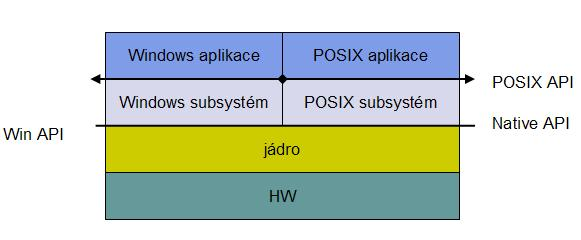
\includegraphics[width=8cm]{informatika/operacne_systemy_a_hw/obrazky/arch-windows.jpg}
  \end{center}
\end{obecne}

\begin{obecne}{Architektura Linuxu}
  \begin{pitemize}
      \item Na �rovni SW -- p�enositelnost; abstrakce HW. 
      \item nad HW~-- kernel, nad n�m syst�mov� vol�n�, hodn� podobn� Windows.
  \end{pitemize}

  \begin{center}
    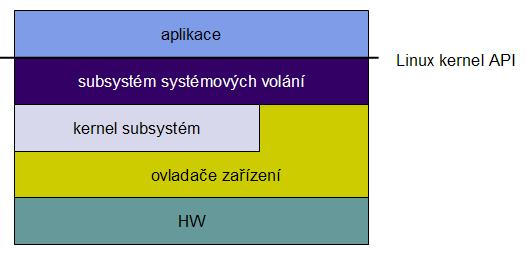
\includegraphics[width=8cm]{informatika/operacne_systemy_a_hw/obrazky/arch-linux.jpg}
  \end{center}
\end{obecne}


\subsection{Vztah OS a HW, obsluha přerušení}

\begin{obecne}{Zjištění změny stavu I/O zařízení:}
\begin{pitemize}
	\item \emph{asynchronní přerušení}~-- zašle zařízení
	\item \emph{polling}~-- peridická kontrola stavu zařízení
\end{pitemize}
\end{obecne}

\begin{obecne}{Druhy přerušení:}
\begin{pitemize}
	\item \emph{synchronní}~-- záměrně (instrukce TRAP~-- vstup do OS), výjimky (nesprávné chování procesu)~-- zpracuje se okamžitě
	\item \emph{asynchronní}~-- vnější událost (např. příchod dat)~-- zpracuje se po dokončení aktuální instrukce 
\end{pitemize}
\end{obecne}

\begin{obecne}{Obsluha přerušení:}
\begin{pitemize}
	\item OS se ujme řízení
	\item uloží se stav CPU (obsah registrů, čítač, ...)
	\item analyzuje se přerušení, vyvolá se příslušná obsluha (pokud není přerušení blokováno)
	\item obslouží se přerušení (např. se zavolá obslužná procedura)
	\item obnoví se stav CPU a aplikace pokračuje, popř. může dojít k přeplánování 
\end{pitemize}
\end{obecne}

\begin{obecne}{I/O software (vrstvy):}
\begin{pitemize}
	\item uživatelský I/O software
	\item I/O nezávislý subsystém
	\item ovladače zařízení
	\item obsluha přerušení 
\end{pitemize}
\end{obecne}

\begin{obecne}{Cíle I/O software:}
\begin{pitemize}
	\item nezávislost zařízení~-- programy nemusí vědět, s jakým přesně pracují
	\item jednotné pojmenování (/dev)
	\item připojení (mount)~-- vyměnitelná zařízení
	\item obsluha chyb
\end{pitemize}
\end{obecne}

\subsection{Procesy, vl�kna, pl�nov�n�}

\subsubsection*{Procesy a vl�kna}
Syst�mov� vol�n� je interface mezi OS (kernelspace) a u��vatelsk�mi programy (userspace).

\begin{e}{Definice}{0}{Proces}
  \emph{Proces} je in�tancia vykon�van�ho programu. Proces m� vlastn�
\textbf{pid (Process ID), pr�va (u�ivatele), adresn� prostor (pam�), vl�kna a otev�en� soubory}.
\end{e}

\obrazekvpravo{informatika/operacne_systemy_a_hw/obrazky/procesy_stavy.png}{P�echody mezi stavy procesu}{}{0.45}
\begin{e}{Stavy procesu}{0}{0}
Po�as �ivota sa m��e proces/vl�kno nach�dza� v r�znych stavoch:
\begin{pitemize}
  \item \emph{be��c�}~-- jeden proces/vl�kno na procesor,
  \item \emph{zablokovan�}~-- pri pou�it� blokuj�ceho volania~-- I/O disku at�.,
  \item \emph{p�ipraven�}~-- skon�ilo blokovanie; spotreboval v�etok pridelen� �as resp. vr�til riadenie syst�mu, �ak� na nov� pridelenie procesora,
  \item \emph{zombie}~-- po ukon�en� procesu, ke� u� nepracuje~-- ale e�te nebol vymazan�\footnote{taky stav zombie tam neni jenom kvuli vtipnosti; kdyz proces skonci
svoji cinnost, tak se treba muze cekat na to, az si navratovou hodnotu
procesu nekdo vyzvedne - a potom se proces muze oznacovat ve stavu
zombie }.
\end{pitemize}
\end{e}

\begin{e}{Organizace pam�ti procesu}{0}{0}

Pam� procesu (spu�t�n�ho programu) lze rozd�lit do n�kolika ��st�:
\begin{pitemize}
\item \emph{k�d programu (text segment)} \\
vytvo�en p�i p�ekladu, sou��st spustiteln�ho souboru, nem�nn� a m� pevnou d�lku; obvykle b�v� chr�n�n proti z�pisu
\item \emph{statick� data (data segment)} -- data programu, jejich� velikost je zn�ma ji� p�i p�ekladu a jejich� pozice se b�hem programu nem�n� (je p�ipraven kompil�torem a jeho form�t je takt� zadr�tovan� ve spustiteln�m souboru, u inicializovan�ch statick�ch dat je tam cel� ulo�en�); v jazyce C jde o glob�ln� prom�nn� a lok�ln� data deklarovan� jako \texttt{static} (prom�nn� alokovan� pouze jednou), konstanty
\item \emph{halda (heap segment)} -- vytv��en startovac�m modulem (C Runtime library), ukl�daj� se sem dynamicky vznikaj�c� objekty (\texttt{malloc, new})  neinicializovan� data, i seznam voln�ho m�sta. \\Halda zjemnuje to, co ti dovoluje spravce virtualni pameti. Ten ti dovoluje taky alokovat pamet a jinak s ni pracovat, ale protoze umi pracovat jen s celymi strankami (treba 4 KB velke), tak proste nekolikabajtove bloky od nej dostat primo nemuzes. A halda prave ty cele alokovane stranky rozdeluje do mensich bloku (postupne z nich ukrajuje, jak volas \texttt{malloc()})... pokud ji volna pamet dojde, alokuje si dalsi stranky... a tak dale.
\item \emph{voln� pam�} \\
postupn� j� zapl�uje z jedn� strany z�sobn�k a z druh� halda
\item \emph{z�sobn�k (stack segment)} \\
informace o vol�n� procedur (\uv{aktiva�n� z�znamy}) --- n�vratov� adresy, parametry a n�vratov� hodnoty (nejsou-li p�ed�v�ny v registrech), n�kter� jazyky (Pascal, C) pou��vaj� i pro �schovu lok�ln�ch prom�nn�ch. Typicky roste z�sobn�k proti hald� (od \uv{konce} pam�ti k ni���m adres�m).
\end{pitemize}
\end{e}

\begin{e}{Definice}{0}{Vl�kno (Thread)}
  \emph{Vl�kno} je mo�nos� pre program ako sa \uv{rozdeli�} na dva alebo viac
  z�rove� (resp. pseudo-z�rove�) vykon�van�ch �loh. Oproti procesu mu nie je
  pridelen� vlastn� pam�~-- je to len miesto vykon�vania in�trukci� v programe.
  Oproti procesu s� jeho \uv{atrib�tmi} len: \textbf{stav(+priorita), z�sobn�k, registrov CPU (i hodnotou PC\footnote{kdy� se vl�kno p�eru�� tak se ulo��
i to kam v n�m PC ukazoval - aby pak mohlo pokra�ovat kde zkon�ilo})}.
\end{e}
\begin{figure}[h]
  \centering
  \subfloat[Process control block]{\label{fig:pcb_process} 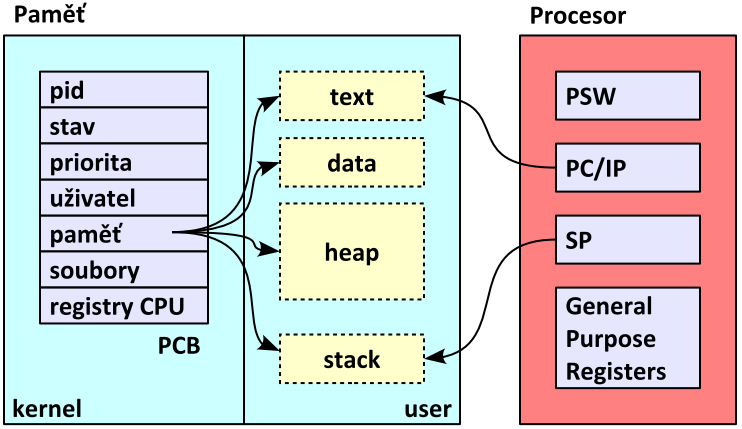
\includegraphics[width=8cm]{informatika/operacne_systemy_a_hw/obrazky/pcb_process_control_block.png}} \hfill
  \subfloat[Process control block s vl�kny]{\label{fig:pcb_thread}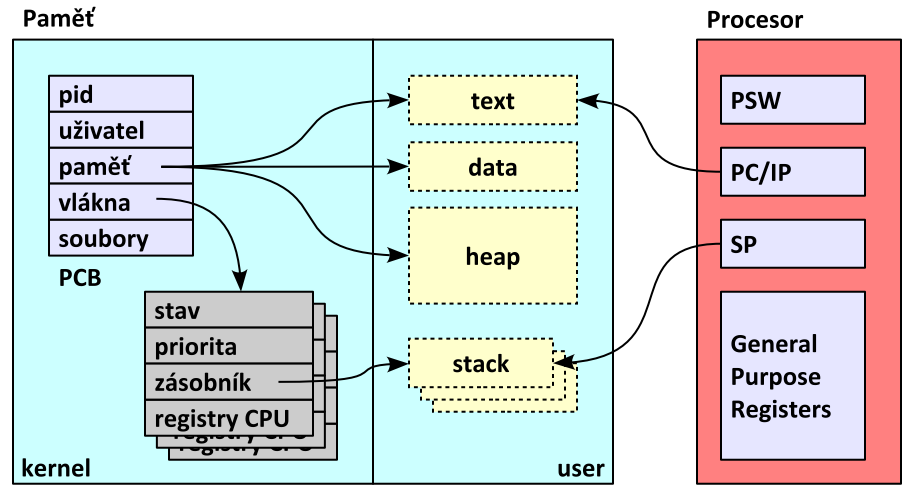
\includegraphics[width=8.5cm]{informatika/operacne_systemy_a_hw/obrazky/pcb_process_control_block_vlakna.png}}
  \caption{Process Control Block - execution context \footnotesize(v�imn�te si
  odd�len�ho kernel a user m�du)}
  \label{fig:pcb}
\end{figure}

\newpage
\textbf{Implementace:}
\begin{pitemize}
        \item \textbf{User Level Threads}(1.diagram) - thread management d�l� aplikace (nemus� b�t podporov�ny OS), ka�d� proces ma thread table, kdy� syst�m zablokuje proces zablokuj� se i v�echny jeho thready
        \item \textbf{Kernel Threads}(2.diagram) - thread management d�l� OS (mus� podporovat), thread table je glob�ln�, syst�m blokuje pouze jednotliv� thready
  \begin{center}
  \begin{center}
    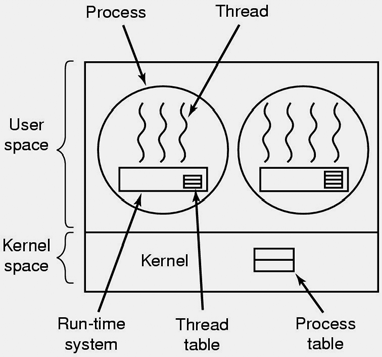
\includegraphics[height=6cm]{informatika/operacne_systemy_a_hw/obrazky/user-threads.png}
    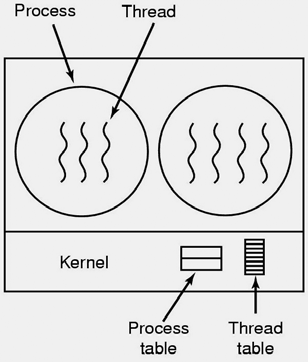
\includegraphics[height=6cm]{informatika/operacne_systemy_a_hw/obrazky/kernel-threads.png}
  \end{center}  
  \end{center}
\end{pitemize}
\emph{Multithreading} - schopnost syst�mu efektivn� pou��vat v�ce thread�, modely:
\begin{pitemize}
        \item \textbf{many-to-one (User Level Threads)} - mnoho user-level thread� je namapov�no na jednu kernel entitu, pou��v� se na syst�mech nepodporuj�c�ch kernel thready (nap�. Linux - GNU Portable Threads)
        \item \textbf{one-to-one (Kernel Threads)} - ka�d� user-level thread je namapov�n na jeden kernel thread (nap�. win2000, Linux - NGPT)
\end{pitemize}

\subsubsection*{Pl�nov�n�}

P�i pl�nov�n� procesoru se v opera�n�m syst�mu \textit{pl�nova�} (anglicky scheduler) rozhoduje, kter�mu procesu bude p�id�len procesor, a tedy kter� proces v n�sleduj�c�m �asov�m �seku bude procesor po��ta�e vyu��vat pro sv�j b�h. K pl�nov�n� procesoru doch�z� v n�sleduj�c�ch situac�ch:
\begin{pitemize}
        \item pokud n�kter� b��c� proces p�ejde do stavu blokovan�
        \item pokud n�kter� proces skon��
        \item pokud je b��c� proces p�eveden do stavu p�ipraven�
        \item pokud je n�kter� proces p�eveden ze stavu blokovan� do stavu p�ipraven�
\end{pitemize}
 Pl�novanie pritom m��e by� \textit{preempt�vn�} (v�t�inou pomoc� p�eru�en�, bez spolupr�ce s programem, pln� v re�ii OS - Windows NT, Linux) alebo \textit{nepreemptivn�} (vy�aduje spolupr�ci s programem, kooperat�vne~-- Windows 3.x).
\\\\
\begin{obecne}{Metriky OS pro pl�nov�n� proces�:}
\begin{pitemize}
 \item doba odezvy (response time, turnaround) -- do ukon�eni procesu, do prvni odezvy
 \item propustnost (throughput) -- po�et dokon�enych uloh za jednotku �asu
 \item vyu�iti procesoru (utilization)
 \item spravedlnost (fairness)
\end{pitemize}
\end{obecne}

\begin{obecne}{Algoritmy:}
\begin{pitemize}
        \item \textbf{First Come First Served (FCFS)}: nepreempt�vny, procesy pl�nov�ny v po�ad�, v jak�m p�ich�zej�, procesy b�� dokud neskon��
  \begin{center}
    \includegraphics[width=8cm]{informatika/operacne_systemy_a_hw/obrazky/fcfs.png}
  \end{center}
        \item \textbf{Round Robin}: preempt�vne roz��renie FCFS, ka�d� proces m� stejn� povolen� �asov� kvantum na b�h, po jeho uplynut� je proces p�esunut na konec fronty
  \begin{center}
    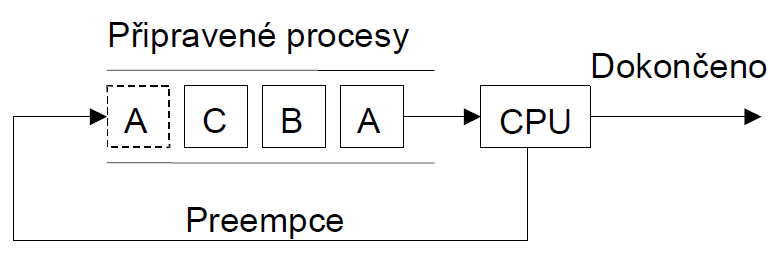
\includegraphics[width=8cm]{informatika/operacne_systemy_a_hw/obrazky/round-robin.png}
  \end{center}
        \item \textbf{Pl�novan� s n�kolika frontami}: ka�d� front� je p�i�azena
n�jak� priorita, bereme procesy s fronty s nejvy��� prioritou. Pokud vy�erp�
svoje �asov� quantum tak j� za�ad�me do fronty o �rove� n�.
  \begin{center}
    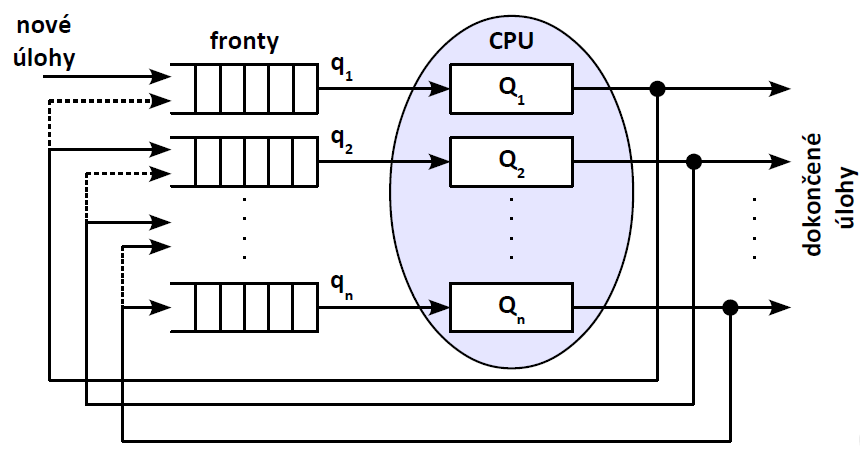
\includegraphics[width=8cm]{informatika/operacne_systemy_a_hw/obrazky/vice-front.png}
  \end{center}

        \item \textbf{Symmetric multiprocessing (SMP)}: druh v�ceprocesorov�ch syst�m�, u kter�ch jsou v�echny procesory v po��ta�i rovnocenn�,  fronta CPU �akaj�cich na pripraven� procesy (akt�vne (spotrebov�va energiu) vs. pas�vne �akanie (�peci�lne in�trukcie)), \uv{vz�ah}/afinita procesov k CPU
        \end{pitemize}
\end{obecne}

\begin{reportN}{Zavoral}
zhruba to co je vo vypiskach, diskusia dalej pokracovala o rozdieloch medzi vlaknami a procesmi - napr ako su implementovane vlakna v OS ktory ich nepodporuje (snazil som sa to nejak ukazat na JVM, ale podrobnosti som velmi nevedel, takze to bolo dost napovedy pana Zavorala a par slov odo mna :? ).
\\\\
n�kdo jiny: som letel na Vlaknach (nevedel som ze su reprezentovane hodnotou registrov, prog. citaca a zasobnikom)
\end{reportN}

\subsection{Synchroniza�n� primitiva, vz�jemn� vylou�en�}

\subsubsection*{Pojmy}

\begin{description}
  \item[�asov� z�visl� chyby (Race Conditions)] Situace kde 2 nebo v�ce proces� p�istupuje ke stejn�mu sd�len�mu prost�edku, a fin�ln� v�sledek z�le�� na kdo prob�hne kdy se jmenuje \emph{race conditions}

  P��klad na tiskov� front�:
  \begin{center}
    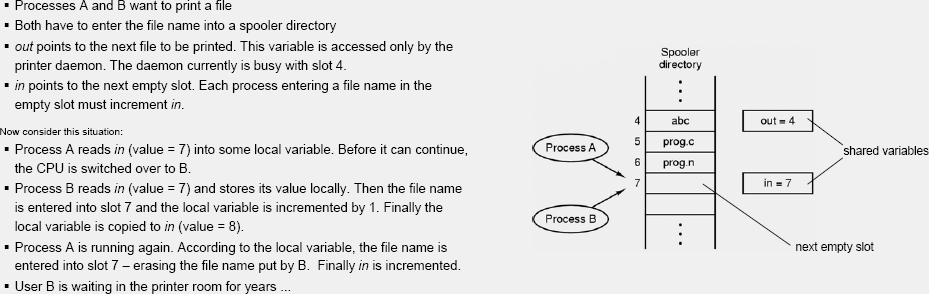
\includegraphics[width=13cm]{informatika/operacne_systemy_a_hw/obrazky/race-conditions.png}
  \end{center}

        \item[Kritick� sekce (Critical Regions)] ��st programu, kter� dokud nen� dokon�ena nen� mo�n� za��t jinou (nap�. pou��v� sd�len� prost�edky)
  \begin{center}
    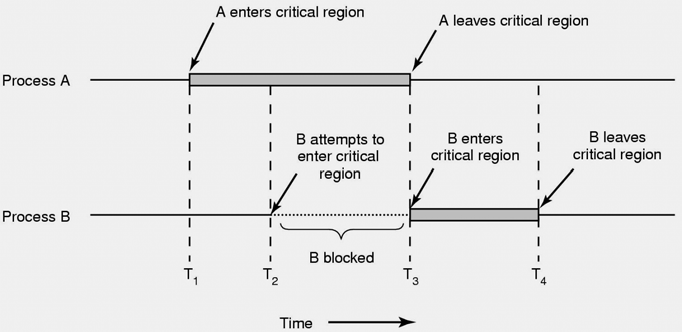
\includegraphics[width=9cm]{informatika/operacne_systemy_a_hw/obrazky/critical-region.png}
  \end{center}  
  
        \item[Vz�jemn� vylou�en� (Mutual Exclusion)] kritickou operaci prov�d� nejv��e jeden proces. Podm�nky vz�jemn�ho vylou�en�:
\begin{penumerate}
        \item ��dn� dva procesy nemohou b�t najednou ve stejn� kritick� sekci
        \item Nemohou b�t u�in�ny ��dn� p�edpoklady o rychlosti procesu (��dn� odhady rychlosti nebo priorit procesu, mus� fungovat se v�emi procesy)
        \item ��dn� proces mimo kritickou sekci nesm� blokovat jin� proces
        \item ��dn� proces nesm� �ekat nekone�n� dlouho v kritick� sekci (jinak dead-lock)
\end{penumerate}
Metody dos�hnut� vz�jemn�ho vylou�en�: aktivn� �ek�n� (busy waiting) a pasivn� �ek�n�/blokov�n�.
\end{description}

\subsubsection*{Aktivn� �ek�n� (Busy Waiting)}
\emph{Vlastnosti}: \textbf{spot�ebov�v� �as procesoru}, vhodn�j�� pro p�edpokl�dan� kr�tk� doby �ek�n�, nespot�ebov�v� prost�edky OS, rychlej��.

Navrhovan� �e�en�: 
\begin{pitemize}
  \item \textbf{Zak�z�n� p�eru�en�}] nevhodn� - proces m� plnou kontrolu nad po��ta�em 
  \item \textbf{Z�mky v prom�nn�}] nefunguj� - mezi p�e�t�n�ma nastaven�m locku m��e b�t program p�eru�en - pak by si "nev�im" lock == 1 a vesel pokra�oval, akor�t jsme p�idali novou race condition. 
\begin{verbatim}
int lock;
void proc(void) {
  for (;;) {
    nekritick�_sekce();
    while (lock != 0);
    lock = 1;
    kritick�_sekce();
    lock = 0;
  }
}
\end{verbatim}
  \item \textbf{D�sledn� st��d�n� (Strict Alternation)} funguje ale poru�uje podm�nku 3 - prom�nn� turn hl�d� kdo je na �ad�

\begin{verbatim}
int turn = 0;

void p1(void)                void p2(void)
{                            {
  for (;;) {                   for (;;) {
    while (turn != 0);           while (turn != 1);
    kritick�_sekce();            kritick�_sekce();
    turn = 1;                    turn = 0;
    nekritick�_sekce();          nekritick�_sekce();
  }                            }
}                            }
\end{verbatim}

  \begin{center}
    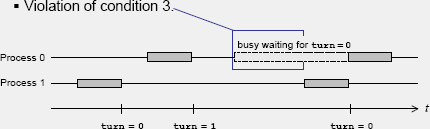
\includegraphics[width=9cm]{informatika/operacne_systemy_a_hw/obrazky/strict-alternation.png}
  \end{center}

\emph{Petersonovo �e�en�} - zobecn�n� pro N proces�:
\begin{verbatim}
#define N 2                   /* po�et proces� */
�
int turn;
int interested[N];            /* kdo m� z�jem */
�
void enter_region(int proc) { /* proc: kdo vstupuje */
int other = 1-proc;             /* ��slo opa�n�ho procesu */
    interested[proc] = TRUE;    /* m�m z�jem o vstup */
    turn = proc;                /* nastav p��znak */
    while (turn == proc && interested[other] == TRUE);
}
�
void leave_region(int proc) { /* proc: kdo vystupuje */
    interested[proc] = FALSE;   /* u� odch�z�m */
}
\end{verbatim}
 
  \item \textbf{Instrukce Test-and-Set Lock (TSL)} - atomick� operace na �rovni strojov�ho k�du, nem��e b�t p�eru�ena je nutn� aby ji podporoval HW (v�echny sou�asn� procesory n�jakou maj�):
\\
- implementace spin-locku (druh z�mku, na n�j� je t�eba aktivn� �ekat � �ekaj�c� proces p�i �ek�n� na spinlock spot�ebov�v� syst�mov� prost�edky) - po��d ale m�n� prost�edk� ne� p�edchoz� �e�en�  
\begin{verbatim}
enter_region:
    tsl   R,lock           ; na�ti z�mek do registru R a    
                           ; nastav z�mek na 1                        
    cmp   R,#0             ; byl z�mek nulov�?
    jnz   enter_region     ; byl-li nenulov�, znova
    ret                    ; n�vrat k volaj�c�mu - vstup do
                           ; kritick� sekce
�leave_region:
    mov   lock,#0          ; ulo� do z�mku 0
    ret                    ; n�vrat k volaj�c�mu
\end{verbatim}
\end{pitemize}

\subsubsection*{Pasivn� �ek�n�}
\emph{Vlastnosti}: proces je ve stavu blokov�n, vhodn� pro del�� doby �ek�n�, \textbf{spot�ebov�v� prost�edky OS}, pomalej��.

Postup pou��vaj�c� Sleep/Wakeup (implementov�ny OS, atomick� operace - sleep usp� volaj�c� proces, wakeup probud� udan� proces) nefunguje (viz Probl�m producent/konzument).
\begin{pitemize}
\item \textbf{Semafory} -- po��t� po�et probuzen�ch, reprezentace voln�ch a p�id�len�ch prost�edk�

Atomick� operace (nesm� b�t p�eru�eny):

\begin{description}
\item[down(semaphore* s)] -- zabere semafor (\verb=s--;=) pokud je voln� (\verb=s>0=), jinak �ek� na uvoln�n�

\item[up(semaphore* s)] -- uvoln� semafor (\verb=s++;=), vzbud� �ekaj�c� proces (pokud existuje)
\end{description}
-nutn� podpora OS (v�t�inou v kernelu)
 

\item \textbf{Mutex}
�peci�lny (bin�rny) typ semaforu, kde s� povolen� len hodnoty 0 a 1 (v Up sa miesto $s:=s+1$ vol� $s:=1$) sa naz�va \emph{mutex} a pou��va sa na riadenie pr�stupu k jednej premennej. V�t�inou pomoc� TSL.

\item \textbf{Monitory}
\par Implementov�ny p�eklada�em, lze si p�edstavit jako t��du C++ (v�echny prom�nn� priv�tn�, funkce mohou b�t i ve�ejn�), vz�jemn� vylou�en� v jedn� instanci (zaji�t�no synchronizac� na vstupu a v�stupu do/z ve�ejn�ch funkc�, synchronizace implementov�na blokovac�m primitivem OS). ???TODO

\item \textbf{Zpr�vy}
\par Operace SEND a RECEIVE, zablokov�n� odes�latele/p��jemce, adresace proces/mailbox, rendez-vous...

\item \textbf{RWL - read-write lock}, \textbf{bari�ry}...

Ekvivalence primitiv - pomoc� jednoho blokovac�ho primitiva lze implementovat jin� blokovac� primitivum.

Rozd�ly mezi platformami: Windows - jednotn� funkce pro pasivn� �ek�n�, �ek�n� na v�ce primitiv, timeouty. Unix - OS implementuje semafor, knihovna pthread.
\end{pitemize}
\subsubsection*{Klasick� synchroniza�n� probl�my}
\begin{pitemize}
\item \textbf{Probl�m producent/konzument}
\par Producent vyr�ba predmety, konzument ich spotreb�va. Medzi nimi je buffer pevnej ve�kosti (N). Konzument nem� �o spotreb�va� ak je buffer pr�zdny; producent prestane vyr�ba�, ak je buffer pln�. 

\begin{verbatim}
int N = 100;
int count = 0;
void producer(void) {
    int item;
    while(TRUE) {
        produce_item(&item);
        if(count==N) sleep ();
        enter_item(item);
        count++;
        if(count == 1) wake(consumer);
    }
}
void consumer(void) {
    int item;
    while(TRUE) {
        if(count==0) /*pozice A*/ sleep ();
        remove_item(&item);
        count--;
        if(count==N-1)
            wake(producer);
        consume_item(&item);
    }
}
\end{verbatim}

\begin{penumerate}
        \item Buffer je pr�zdny, a konzument pr�ve pre��tal count, aby zistil, �i je rovn� nule
        \item Prepl�novanie na producenta ("pozice A")
        \item Producent vytvo�� item a zv��� count
        \item Producent zist�, �i je count rovn� jednej. Zist� �e �no, �o znamen� �e konzument bol predt�m zablokovan� (preto�e muselo by� 0), a zavol� wakeup
        \item Teraz m��e d�js� k zablokovaniu: konzument pokra�uje na "pozici
A" a usp� se, preto�e si mysl�, �e nem� �o zobra�; producent bude chv��u produkova� a d�jde "preplneniu" $\Rightarrow$ usp� sa; sp� producent aj konzument :o) 
\\\\
�e�en� pomoc� semaforu:\\
\begin{verbatim}
#define N 10
typedef int semaphore;     //a semaphore is an integer
semaphore empty = N;       //counting empty slots
semaphore full = 0;        //counting full slots
semaphore mutex = 1;       //mutual exclusion on buffer access

void producer() {
  while (TRUE) {
    int item = produce_item();
    down(&empty);          //possibly sleep, decrement empty counter
    down(&mutex);          //possibly sleep, claim mutex (set it to 0) thereafter
    insert_item(item);
    up(&mutex);            //release mutex, wake up other process
    up(&full);             //increment full counter, possibly wake up other ...
  }
}

void consumer() {
  while(TRUE) {
    down(&full);           //possibly sleep, decrement full counter
    down(&mutex);          //possibly sleep, claim mutex (set it to 0) thereafter
    item = remove_item();
    up(&mutex);            //release mutex, wake up other process
    up(&empty);            //increment empty counter, possibly wake up other ...
    consume_item(item);
  }
}
\end{verbatim}

\end{penumerate}
\item \textbf{Probl�m ob�dvaj�c�ch filosof�}
\par P�t filosof� sed� okolo kulat�ho stolu. Ka�d� filosof m� p�ed sebou tal�� �paget a jednu vidli�ku. �pagety jsou bohu�el slizk� a je t�eba je j�st dv�ma vidli�kami. �ivot filosofa sest�v� z obdob� j�dla a obdob� p�em��len�. Kdy� dostane hlad, pokus� se vz�t dv� vidli�ky, kdy� se mu to poda��, naj� se a vidli�ky odlo��.

\item \textbf{Probl�m ospal�ho holi�e}
\par Holi� m� ve sv� ofic�n� k�eslo na holen� z�kazn�ka a pevn� po�et seda�ek pro �ekaj�c� z�kazn�ky. Pokud v ofic�n� nikdo nen�, holi� se posad� a sp�. Pokud p�ijde prvn� z�kazn�k a holi� sp�, probud� se a posad� si z�kazn�ka do k�esla. Pokud p�ijde z�kazn�k a holi� u� st�ih� a je voln� m�sto v �ek�rn�, posad� se, jinak odejde.
\end{pitemize}


\begin{reportN}{Bulej}
\begin{penumerate}
        \item priklad Producent-konzument pomoci semaforu

        \item stacilo napsat aktivni vs. pasivni, kriticka sekce, spinlock, semafor (obecne monitor) a pak nasledovalo par otazek, zda je mozne naprogramovat synch. primitivum bez podpory HW
\end{penumerate}
\end{reportN}

\begin{reportN}{Bulej}
Mysl�m, �e jsem je pochopil, a� kdy� mi to pan Skopal vysv�tlil. To, co je v materi�lech opravdu nesta��. TSL je dobr� v tom, �e m� prav� operaci Test and Set Lock jako atomickou. Pak jsem se pokou�el ud�lat semafor pro probl�m producent a konzument a d�lal jsem ho upln� �patn�
\end{reportN}

\begin{reportN}{Hn�t�nka}
na jedni�ku mus�te um�t praktick� u�it� (nap�. z v�ce mutex� postavit semafor)
\end{reportN}

\begin{reportN}{Bedn�rek}
Na tuhle jsem byl p�ipraven� ze zadan�ch ot�zek asi nejh��, kupodivu jsem toho k n� ale nakonec na pap�r vyplodil pom�rn� dost a dostal k t�matu jen m�lo dopl�uj�c�ch ot�zek (n�jak� drobn� praktick� a jak implementovat mutex bez podpory OS, tj. pomoc� test-and-set instrukce), pak se plynule a nepozorovan� p�e�lo na zablokov�n� a zotaven� z n�j. N�co jsem v�d�l, vzpomn�l jsem si na 3 ze 4 Coffmanov�ch podm�nkek a jejich o�et�en�, �tvrtou jsem pak vymyslel s Bedn�rkovou vydatnou pomoc�. ��dn� ot�zky na "klasick� synchroniza�n� probl�my" nebo Petersonovo �e�en�, tj. v�ci, o kter�ch jsem se s�m rad�i nezm�nil.

na konci sa opytal, ze aky problem okrem vyhladovania moze nastat... deadlock

Sleep/wakeup, semafory, monitory, spr�vy, polling - u ka�d�ho ako funguje a �i to rob� aplik�cia/OS/HW. Potom sme sa pobavili o mo�nosti implementova� jedno druh�m. 
\end{reportN}

\subsection{Zablokov�n� a zotaven� z n�j}

Prost�edek je cokoliv, k �emu je pot�eba hl�dat p��stup (HW za��zen�~-- tisk�rny, cpu; informace~-- z�znamy v DB). Je mo�n� je rozd�lit na \emph{odn�mateln�} (lze odejmout procesu bez n�sledk�~-- CPU, pam�) a \emph{neodn�mateln�} (nelze odejmnout bez nebezpe�� selh�n� v�po�tu~-- CD-ROM, tisk�rna... tento druh zp�sobuje probl�my).

Pr�ce s prost�edky prob�h� v n�kolika kroc�ch: \emph{��dost o prost�edek} (blokuj�c�, pr�v� tady doch�z� k zablokov�n�), \emph{pou��v�n�} (nap�. tisk), \emph{odevzd�n�} (dobrovoln�/p�i skon�en� procesu).

Mno�ina proces� je \emph{zablokov�na}, jestli�e ka�d� proces z t�to mno�iny �ek� na ud�lost, kterou m��e zp�sobit pouze jin� proces z t�to mno�iny.

\subsubsection*{Coffmanovy podm�nky}
Splnenie t�chto podmienok je nutn� pre zablokovanie:
\begin{penumerate}
	\item \textbf{V�lu�n� p��stup} � ka�d� prost�edek je bu� vlastn�n pr�v� jedn�m procesem nebo je voln�.
	\item \textbf{Dr� a �ekej} � procesy aktu�ln� vlastn�c� n�jak� prost�edky mohou ��dat o dal��.
	\item \textbf{Neodn�matelnost} � p�id�len� prost�edky nemohou b�t proces�m odebr�ny.
	\item \textbf{�ek�n� do kruhu} � existuje kruhov� �et�z proces�, kde ka�d� z nich �ek� na prost�edek vlastn�n� dal��m �l�nkem �et�zu.
\end{penumerate}

\subsubsection*{�e�en� zablokov�n�}
\begin{pitemize}
	\item \textbf{P�tros� algoritmus}~-- Zablokov�n� se ani nedetekuje, ani se mu nezabra�uje, ani se neodstra�uje, U�ivatel s�m rozhodne o �e�en� (kill). Nespot�ebov�v� prost�edky OS~-- nem� re�ii ani neomezuje podm�nky provozu. (Nej�ast�j�� �e�en�~-- Unix, Windows) 
  \item \textbf{Detekce a zotaven�}~-- Hled� kru�nici v orientovan�m grafu (hrany vedou od procesu, kter� �ek�, k procesu, kter� prost�edek vlastn�), pokud tam je kru�nice, nastalo zablokov�n� a je t�eba ho �e�it:
		\begin{pitemize}
			\item \emph{Odebr�n� prost�edku}~-- dohled oper�tora, pouze na p�echodnou dobu
			\item \emph{Zab�jen� proces� z cyklu} (resp. mimo cyklus vlastn�c� identick� prost�edek)
			\item \emph{Rollback} (OS ukl�d� stav proces�, p�i zablokov�n� se n�kter� procesy vr�t� do p�edchoz�ho stavu $\Rightarrow$ ztracena pr�ce... obdoba u DB)
		\end{pitemize}
	\item \textbf{Vyh�b�n� se}~-- Bezpe�n� stav (procesy/prost�edky nejsou zablokov�ny, existuje cesta, jak uspokojit v�echny po�adavky na prost�edky spou�t�n�m proces� v jist�m po�ad�); Vi�. bank���v algoritmus. Nutn� je p�edem zn�t v�echny prost�edky, kter� budou programy pot�ebovat; OS pak d�v� prost�edky tomu, kter� je nejbl� sv�mu maximu pot�eby a nav�c pro kter� je prost�edk� dost na dokon�en�. Dnes se moc nepou��v�.
	\item \textbf{P�edch�zen� (prevence)}~-- napaden� jedn� z Coffmanovy podm�nek
		\begin{penumerate}
			\item \emph{V�lu�n� p��stup}~-- \emph{spooling} (prostriedky spravuje jeden systemov� proces, ktory dohliada na to, aby jeho stav bol konzistentny (tiskarna)~-- pozor na m�sto na disku)
			\item \emph{Dr� a �ekej}~-- ��dat o v�echny prost�edky p�ed startem procesu. Nejprve v�echno uvolnit a pak znovu ��dat o v�echny najednou
			\item \emph{Neodn�matelnost}~-- odn�mateln� prost�edky mohou b�t odejmuty bez n�sledk� (procesor-p�epl�nov�n�, pam�-swapping), neodn�mateln� nelze bez nebezpe�� selh�n� v�po�tu
			\item \emph{�ek�n� do kruhu}~-- v�echny prost�edky jednozna�n� o��slov�ny (sta�� prost�edky v n�jak�m kontextu), procesy mohou ��dat o prost�edky jen ve vzestupn�m po�ad�

		\end{penumerate}
			\item \emph{Dvojf�zov� zamyk�n�}~-- nejprve postupn� v�echno zamyk�m (prvn� f�ze). Potom se m��e pracovat se zam�en�mi prost�edky~-- a na z�v�r se u� jen odemyk� (druh� f�ze)~-- vi� transak�n� spracov�n� u datab�z� ((striktn�/konzervativn�) dvouf�zov� zpracov�n�)
\end{pitemize}

\textbf{Bank���v algoritmus}: Bank�� m� klienty a t�m sl�bil jistou v��ku �v�ru. Bank�� v�, �e ne v�ichni klienti pot�ebuj� plnou v��i �v�ru najednou. Klienti ob�as nav�t�v� banku a ��daj� postupn� o prost�edky do maxim�ln� v��ky �v�ru. A� klient skon�� s obchodem, vr�t� bance vyp�j�en� pen�ze. Bank�� pen�ze p�j�� pouze tehdy, z�stane-li banka v bezpe�n�m stavu.
\\ Probl�my: slo�itost $O(N^2)$, po�adovan� info je typicky nedostupn�, efektivn�j�� b�v� �e�it a� vznikl� probl�my
\subsection{Organizace pam�ti, aloka�n� algoritmy}

\textbf{Hierarchie pam�ti} (sm�rem odshora dol� roste velikost, cena na bajt a rychlost kles�~-- a naopak\dots):
\begin{pitemize}
    \item \emph{registry CPU} --- 10ky-100vky bajt� (IA-32: obecn� registy p�r 10tek), IA-64~-- a� kB (extr�m), stejn� rychl� jako CPU. 
    \item \emph{cache} --- z pohledu aplikac� nen� p��mo adresovateln�; dnes ��dov� MB, rozd�len� podle ��elu, n�kolik vrstev. L1 cache (cca 10ky kB)~-- d�len� instrukce/data; L2 (cca MB) sd�len� instr\&data, b�� na rychlosti CPU (d��v b�vala pomalej��), servery~-- L3 (cca 10MB). Vyrovn�v� rozd�l rychlosti CPU a RAM. Vyu��v� lokality program� -- cyklen� na m�st�; sekven�n�ho p��stupu k dat�m. Pokud nenajdu co chci v cache -- \uv{cache-miss}, na��t� se pot�ebn� z RAM (po bloc�ch), jinak (v 95-7\% p��pad�) nastane \uv{cache-hit}, tj. po�adovan� data v cache opravdu jsou a do RAM nemus�m.
    \item \emph{hlavn� pam�} (RAM) --- p��mo adresovateln� procesorem, 100MB~-- GB; pomalej�� ne� CPU; CAS~-- doba p��stupu na ur�. m�sto~-- nejv�c zdr�uje (v 1 sloupci u� �te rychle, dat. tok dostate�n�), dal��~-- latence~-- doba ne� data dote�ou do CPU~-- hraje roli vzd�lenost (AMD- integrovan� �adi� v CPU) 
    \item \emph{pomocn� pam�} --- nen� p��mo adresovateln�, typicky HDD; n�h. p��stup, ale pomalej��. ~100GB, r�zn� druhy~-- IDE, SATA, SCSI; nejv�c zdr�uje p��stupov� doba (�as seeku) cca 2-10ms; obvykle sektor~-- 512 B; roli hraje i rychlost ot��en� (4200~-- 15000 RPM)~-- taky ��dov� ms. 
    \item \emph{z�lohovac� pam�} --- nejpomalej��, z teorie nejv�t��, dnes ale neplat�; typicky~-- p�sky; pro v�t�� kapacitu~-- autoloadery ; sekven�n� p��stup; dnes~-- kv�li rychlosti �asto z�lohov�n� RAIDem.
\end{pitemize}

\textbf{Spr�vce pam�ti}: ��st OS, kter� spravuje pam�ovou hierarchii se naz�v�\\spr�vce pam�ti (memory manager):
\begin{pitemize}
	\item udr�uje informace o voln�/pln� ��sti pam�ti
	\item star� se o p�id�lov�n� pam�ti
	\item a \uv{v�m�nu pam�ti s diskem}
\end{pitemize}

\textbf{P�i�azen� adresy}
\begin{pitemize}
	\item p�i p�ekladu (je ji� zn�mo um�st�n� procesu, generuje se absolutn� k�d, PS: statick� linkov�n�)
	\item p�i zav�d�n� (OS rozhodne o um�st�n�~-- generuje se k�d s relokacemi, PS: dynamick� linkov�n�)
	\item za b�hu (proces se m��e st�hovat i za b�hu, reloka�n� registr)
\end{pitemize}

\textbf{Overlay}~-- Proces pot�ebuje v�ce pam�ti ne� je skute�n� k dispozici.
Program�tor tedy rozd�l� program na nez�visl� ��sti (kter� s v pam�ti podle
pot�eby vym��nuj�) a ��st nezbytnou pro v�echny ��sti... Pou��v�no hlavn� v DOSu, nyn� se stejn�ho c�le dosahuje pomoc� virtu�ln� pam�ti

\textbf{V�m�na (swapping)}~-- d�l� se, proto�e proces mus� b�t v hlavn� pam�ti,
aby jeho instrukce mohly b�t vykon�v�ny procesorem... Jde o v�m�nu obsahu pam�ti
mezi hlavn� a z�lo�n�.

\textbf{P�eklad adresy}~-- nutn�, proto�e proces pracuje v logick�m (virtu�ln�m) adresov�m prostoru, ale HW pracuje s fyzick�m adresov�m prostorem...

\textbf{Spojit� p�id�lov�n� pam�ti}~-- p�id�len� jednoho bloku / v�ce pam�tov�ch odd�l� (\emph{pevn�}~-- pam� pevn� rozd�lena na ��sti pro r�zn� velikosti blok�/\emph{voln�}~-- v libovoln� ��sti voln� pam�ti m��e b�t alokov�n libovoln� velik� blok)

\textbf{Informace o obsazen� pam�ti}~-- bitov� mapa / spojov� seznam voln�ch blok� (spojov�n� uvoln�n�ho bloku se sousedy)

\textbf{Aloka�n� algoritmy}:
\begin{pitemize}
	\item \emph{First-fit}~-- prvn� voln� dostate�n� velikosti~-- rychl�, ob�as ale rozd�l� velkou d�ru
	\item \emph{Next-fit}~-- dal�� voln� dostate�n� velikosti, za��n� se na podledn� prohled�van� pozici~-- jako First-fit, ale rychlej��
	\item \emph{Best-fit}~-- nejmen�� voln� dostate�n� velikosti~-- pomal� (prohled�v� cel� seznam), zanech�v� malink� d�ry (ale nech�v� velk� d�ry vcelku)
	\item \emph{Worst-fit}~-- nejv�t�� voln�~-- pomal� (prohled�v� cel� seznam), rozd�l� velk� d�ry
	\item \emph{Buddy syst�m}~-- pam� rozd�lena na bloky o velikosti $2^n$, bloky stejn� velikosti v seznamu, p�i p�id�len� zaokrouhlit na nejbli��� $2^n$, pokud nen� voln�, roz�t�pnou se v�t�� bloky na p��slu�n� men�� velikosti, p�i uvoln�n� pam�ti se slu�uj� sousedn� bloky (buddy)
\end{pitemize}

\textbf{Fragmentace pam�ti}:
\begin{pitemize}
	\item \emph{extern�}~-- voln� prostor rozd�len na mal� kousky, pravidlo 50\% -- po n�jak� dob� b�hu programu bude cca 50\% pam�ti fragmentov�no a u toho to z�st�v� - pl�tv�n� m�stem mezi alokovan�mi oblastmi
	\item \emph{intern�}~-- nevyu�it� cel�ho p�id�len�ho prostoru (50\% velikosti posledn�ho bloku prostoru nevyu�ito) - pl�tv�n� m�stem uvnit� alokovan� oblasti
	\item \emph{sesyp�n�}~-- pouze p�i p�i�azen� adresy za b�hu, nebo segmentaci~-- nelze p�i statick�m p�id�len� adresy
\end{pitemize}

\subsection{Principy virtu�ln� pam�ti, str�nkov�n�, algoritmy pro v�m�nu str�nek, v�padek str�nky, str�nkovac� tabulky, segmentace}

\subsubsection*{Virtu�ln� pam�}

\obrazekvpravominipage{informatika/operacne_systemy_a_hw/obrazky/virtual-memory.png}{Virtu�l\-n�
pam�}{fig:virpamet}{0.15}{0.8}{

Virtu�ln� pam� zp�sob spr�vy opera�n� pam�ti po��ta�e, kter� umo��uje p�edlo�it b��c�mu procesu adresn� prostor pam�ti, kter� je uspo��d�n jinak nebo je dokonce v�t��, ne� je fyzicky p�ipojen� opera�n� pam� RAM. Z tohoto d�vodu procesor rozli�uje mezi virtu�ln�mi adresami (pracuj� s nimi strojov� instrukce, resp. b��c� proces) a fyzick�mi adresami pam�ti (odkazuj� na konkr�tn� adresov� bu�ky pam�ti RAM). P�evod mezi virtu�ln� a fyzickou adresou je zaji��ov�n samotn�m procesorem v MMU (je nutn� hardwarov� podpora) nebo samostatn�m obvodem. 
\\\\
�lo
by to bez HW podpory? Jist� �e ano VM to tak d�laj�, nicm�n� rychlost nen�
nijak os�uj�c�, proto se do novych stroj� u� p�id�v� jejich HW podpora (??
ov��it).
\begin{pitemize}
        \item Umo��uje sd�len� pam�ti (opera�n�m syst�mem)
        \item Vz�jemn� ochrana program� (v sou�asnosti je d�le�it�j�� ochrana dat ne� vyu�it�
principu lokalit), tzn. to aby jeden program nep�episoval druh�mu programu jeho
data a tak.
        \item Ka�d� b��c� program pracuje se \textbf{sv�m} virtu�ln�m adresn�m prostorem
\end{pitemize}
Existuj� dv� z�kladn� metody implementace virtu�ln� pam�ti � str�nkov�n� a segmentace.
}

\subsubsection*{Str�nkov�n�}
P�i str�nkov�n� je pam� rozd�lena na v�t�� �seky stejn� velikosti, kter� se naz�vaj� str�nky. Spr�va virtu�ln� pam�ti rozhoduje samostatn� o tom, kter� pam�ov� str�nka bude zavedena do vnit�n� pam�ti a kter� bude odlo�ena do odkl�dac�ho prostoru (swapu).
\\\\
Podporovan� v�emi velk�mi CPU a OS, jednorozm�rn� VAP (virtu�ln� adresn�
prostor).\begin{pitemize}
\item VAP rozd�len na str�nky (velikost je mocnina 2), FAP na r�mce (�seky stejn� d�lky)
\item \textbf{p�evod str�nkovac� tabulkou}  - ka�d� proces m� svoj�, p��znak existence mapov�n� (v.str�nka nen� v FAP \rightarrow$ ud�lost "v�padek str�nky" \rightarrow$ synchronn� p�eru�en�) um�st�na v fyzick� pam�ti
\par \begin{center}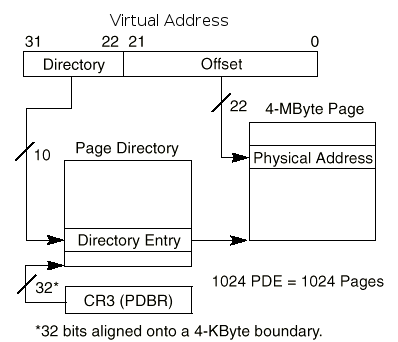
\includegraphics[width=5cm]{informatika/operacne_systemy_a_hw/obrazky/strankovani1_new.png}\end{center}
\item umo�nuje \emph{odd�len� VAP} i \emph{sd�lenou pam�} - mapov�n� virtu�ln� str�nky 2 proces� na jednu fyzickou
\item OS m�n� tabulky str�nek zm�nou PTBR (Page Table Base Register) - PTBR obsahuje
b�zovou adresu tabulky str�nek procesu
\item P��klad: polo�ka str�nkovac� tabulky Intel IA32 (= x86) $\rightarrow$ jej� struktura je z�visl� na architektu�e CPU
\par \begin{center} \includegraphics[width=6cm]{informatika/operacne_systemy_a_hw/obrazky/strankovani-polozka.png} \end{center}
\item \textbf{v�ce�rov�ov� str�nkov�n�} (nap�. kv�li velikosti - jedna tabulka
je u� moc velk� =\textgreater pomal�)
\par \begin{center} \includegraphics[width=6cm]{informatika/operacne_systemy_a_hw/obrazky/strankovani2_new.png} \end{center}
\item \textbf{TLB (Translation Lookaside Buffer)} - asociativn� pam� slou��c� na rychl�  mapov�n� virtu�ln� str�nky na fyzickou, vyhled�v� se v n� paraleln�, typicky ma 128-256 polo�ek, vyu��v� princip prostorov� lokality program� (v�t�ina program� prov�d� velk� po�et p��stup� k mal�mu
po�tu str�nek)
um�st�va v�t�inou v L1 nebo L2 cache na procesoru
\par 
\includegraphics[width=6cm]{informatika/operacne_systemy_a_hw/obrazky/strankovani-tlb-schema.png}
\caption{~~~}
\includegraphics[width=5cm]{informatika/operacne_systemy_a_hw/obrazky/strankovani-tlb.png}
 
\par ...\textbf{0-�rov�ov� str�nkov�n�} - procesor hled� pouze TLB, zbytek
�e�� OS (obl�ben� u 64-bitov�ch CPU - UltraSPARC III)
\item \textbf{inverzn� str�nkov�n�} (nap�. kdy� FAP je men�� ne� VAP, 64-bitov� CPU - IA-64 = UtraSPARC, PowerPC)
- inverzn� str�nkovac� tabulka (IPT) nad r�mci (nikoliv str�nkami) spole�n�
pro v�echny procesy, pro vyhled�v�n� se pou��v� hashovac� tabulka\par \begin{center} \includegraphics[width=10cm]{informatika/operacne_systemy_a_hw/obrazky/strankovani-inv_new.png} \end{center}
\end{pitemize}

\begin{obecne}{Akce vykon�van� p�i v�padku str�nky:}
\begin{pitemize}
\item v�jimka procesoru
\item ulo�it stav CPU (kontext)
\item zjistit VA
\item kontrola platnosti adresy a pr�v
\item nalezen� vhodn�ho r�mce
\item zru�it mapov�n� na nalezen� r�mec
\item pokud je vyhazovan� r�mec vyhazov�n, spustit ukl�d�n� na disk
\item na��st z disku po�adovanou str�nku do r�mce
\item zav�st mapov�n�
\item obnovit kontext
\end{pitemize}
\end{obecne}

\begin{obecne}{P�i implementaci str�nkov�n� je nutno brat v �vahu:}
\begin{pitemize}
    \item \emph{znovuspu�t�n� instrukce} --- je pot�eba aby procesor po v�padku zkusil p��stup do pam�ti znova. dnes um� v�echny CPU, nap�. 68xxx - probl�my (p�eru�en� v p�lce instrukce)
    \item \emph{sd�len� str�nek} --- jednomu r�mci odp. v�c str�nek $\rightarrow$ pokud s n�m n�co d�l�m, t�k� se to v�ech str�nek! mus�m v�e ost. odmapovat. mus�m si pamatovat mapov�n� pro ka�d� r�mec - obr�cen� tabulky.
\item \emph{velikost str�nek} \begin{pitemize} \item velk� str�nky $\rightarrow$ fragmentace
\item mal� str�nky $\rightarrow$ mnoho registr�, zvy�uje cenu v�po�t� a zpomaluje
chod
\item optimum 1-4kB\footnote{4kB se pou��vaj� kvuli jednoduch�mu p�evodu
na fyzickou adresu pomoc� substituce (DRAM mely temer vzdy na cipu N ��dku
x 4096 sloupcu), 64bit procesory umo��uj� pagesize a� 1GB - doporucuju precist
\url{http://www.gamedeception.net/threads/212-The-Importance-of-the-4KB-Page-Boundary}}
\end{pitemize}
    \item \emph{odstran�n� polo�ky z TLB p�i ru�en� mapov�n�} --- nesta�� zm�nit tabulky, mus� se vyhodit i z TLB (kde to m��e, ale nemus� b�t). probl�m - u multiprocesor� m� ka�d� CPU vlastn� TLB, tabulky jsou sd�len� $\rightarrow$ CPU p�i ru�en� mapov�n� mus� poslat interrupt s rozkazem ke smaz�n� v�em (i sob�), po�kat na potvrzen� akce od v�ech.
\end{pitemize}
\end{obecne}
\begin{prikladN}{
Uva�ujte procesor, kter� podporuje str�nkovani, m� dvou�rovnove str�nkovaci tabulky, velikost virtu�ln� i fyzick� adresy 32 bitu, velikost str�nky 4 kB. Nakreslete form�t strankovac� tabulky (polo�ky pot�ebn� pro p�eklad adresy i typick� dal�� p��znakov� bity,
nezadan� detaily rozumne zvolte) a v nem ilustrujte, jak se prelozi virtu�lni adresa 12345678h
(nezadan� konstanty tvoric� konkr�tn� obsah tabulky opet rozumne zvolte).}
Pozn.: h nakonci znamen� �e je ��slo v hex (assembler)
\end{prikladN}

\subsubsection*{Algoritmy pro v�m�nu str�nek (v�b�r ob�ti)}
\begin{pitemize}
\item \textbf{Optim�ln� str�nka} (v okam�iku v�padku str�nky vyb�r�m str�nku, na n� se p�istoup� za nejv�t�� po�et instrukc�) - nelze implementovat
\item \textbf{\uline{NRU}} (Not Recently Used) - ka�d� str�nka m� p��znaky Accessed a Dirty (typicky implementovateln� v HW, mo�no simulovat SW); jednou za �as se sma�ou v�echna A; p�i v�padku rozd�l�m str�nky podle A,D a vyberu str�nku z nejni��� (0,1..4) nepr�zdn� t��dy:
\par \begin{center}
\begin{tabular}{|c|c|c|}
\hline
& A & D \\
\hline
0 & 0 & 0 \\
\hline
1 & 0 & 1 \\
\hline
2 & 1 & 0 \\
\hline
3 & 1 & 1 \\
\hline
\end{tabular}
\end{center}
\item \textbf{\uline{FIFO}} - vyhodit nejd�le namapovanou str�nku - vykazuje anom�lie - Belady (zv�t�en� po�tu v�padk� str�nky, kdy� zv���me po�et str�nek v pam�ti), druh� �ance (�prava FIFO; pokud A=1, za�ad�m na konec FIFO... nevykazuje anom�lie)
\item \textbf{Hodiny} - modifikace druh� �ance: kruhov� zoznam str�nek + iter�tor na ukazuj�c� na nejstar�� str�nku v zoznamu. P�i v�padku (a neexistenci vol�ho r�mce) se zjist�, jestli m� *iterator nastaven� p��znak Accessed. Jestli ne, tato str�nka bude nahrazena - v opa�n�m p��pad� se Accessed p��znak zru�� a iterator++. Toto se opakuje, dokud nedojde k v�m�n�\dots
\item \textbf{LRU} (Least Recently Used) - �asto pou��van� str�nky v posledn�m kr�tk�m �asov�m ��eku budou znovu pou�ity, ��ta� pou�it� str�nek, mo�n� implementovat v HW
\item \textbf{NFU} (Not Frequently Used) - SW simulace LRU, SW ��ta� ke ka�d� str�nce; jednou za �as projdu v�echna A a p�i�tu je k odpov�daj�c�m ��ta��m; vyb�r�m str�nku s nejni���m ��ta�em; nezapom�n� - je mo�n� modifikace se st�rnut�m ��ta�e
\end{pitemize}

\subsubsection*{Segmentace}
dnes pouze Intel IA-32, dvojrozm�rn� VAP
\begin{pitemize}
\item rozd�len� programu na segmenty (napr. podle ��st� s r�zn�mi vlastnostmi - k�d, data, z�sobn�ky\dots), r�zn� d�lky segment�, ktor� m��ou m�nit svoji d�lku za b�hu
\item VAP dvourozm�rn� (segment, offset), FAP jednorozm�rn� (vyzer� jako p�i spojit�m prid�lov�n� pam�ti)
\item segmentov� p�evodn� tabulka (VA se skl�d� ze dvou �ast� S:D, v tabulce se najde adresa segmentu S\dots k t�to adrese se pot� p�i�te D, co je um�stn�n� adresy v FA), p��znak existence mapov�n�
\item p�i v�padku je nutn� m�nit cel� segment (ty mohou b�t velk�), je mo�n� segmenty sesypat - ale nelze m�t segment v�t�� ne� FAP
\end{pitemize}

Segmentaci je mo�n� kombinovat se str�nkov�n�m (odstra�uje nev�hody segmentace, neprov�d� se v�padky segment�):
\par \begin{center}\includegraphics[width=12cm]{informatika/operacne_systemy_a_hw/obrazky/segmentace-a-strankovani.png}\end{center}

\begin{reportN}{Bedn�rek}
T�eba m� p�ekvapila Bedn�kova ot�zka u jedno�rov�ov�ho str�nkov�n�, kdy� se zeptal, co z toho d�l� OS a co procesor (jako co je d�l�no hardwareov� a co softwareov�).
\end{reportN}
\begin{reportN}{Bulej}
Strankovaci tabulku ma kazdy proces vlastni -> ochrana pameti, nemuze pristoupit na cizi stranky (mozna ze to v materialech ke statnicim je, ale ja to z nich nepochopil...)
\end{reportN}
\begin{reportN}{Skopal}
Nejdriv jsem popsal k cemu to je a potom princip. Chtel popsat postup toho co se deje, kdyz se hleda nejaky pointer. Co dela HW, co OS. Pak se zeptal jestli by slo udelat strankovani bez HW podpory (coz rozumne nejde, muselo by se to resit i v prekladacich a bylo by to nefektivni). Pak se zeptal na algoritmy vyhazovani stranek. Popsal jsem FIFO a NRU a to mu stacilo. Na segmentaci nastesti nedoslo.
Celkove velmi prijemne zkouseni. V zasade se spokojil s principy a nestoural moc do detailu.
\end{reportN}
\begin{reportN}{Kofron}
klasika, pre�o, kde, ako ... pre�o to funguje, �o sa rob� pri v�padku str�nky, pre�o dve in�tancie jedn�ho programu nelez� do kapusty aj ke� pracuj� s rovnak�mi virtu�lnymi adresami (ka�d� m� vlastn� str. tabu�ku), tvar adresy, prevody...


ka�d� proces m� vlastn� tabulku, jej� adresa v registru
\end{reportN}
\begin{reportN}{IOI 21. 6. 2011}
Dan� procesor pou��v� 32-bitovou architekturu a dvou�rov�ov� str�nkov�n�.
Instrukce MOV[0x12345678], EAX zapisuje obsah registru EAX na adresu 0x12345678.
Popi�te, jak� operace (p��stupy do registr� a podobn�) vykon�v� p�i prov�d�n� t�to instrukce procesor a jak p�i tom spolupracuje opera�n� syst�m. Rozeberte v�echny mo�n� (z hlediska napln�n� str�nkovac�ch tabulek) p��pady, nepopisujte strategie v�m�ny str�nek.
\end{reportN}

\begin{reportN}{Yaghob} mel ruzn� dotazy, jako proc je str�nka velik� zrovna 4kB, jak je to se str�nkov�n�m na 64-bitov�ch procesorech 
\end{reportN}

\subsection{Syst�my soubor�, adres��ov� struktury}

\begin{e}{Definice}{0}{Syst�my soubor�}
  \begin{pitemize}
    \item Poskytuj� jednotn� rozhran� pro �ten� a ukl�d�n� dat z/do pomocn�ch pam�t�
(sekund�rn�, terci�ln�).
    \item Skr�vaj� povahu za��zen�, na kter�m jsou um�st�ny. Aplikace s t�mto za��zen�m mohou
pracovat pouze p�es rozhran� souborov�ho syst�mu, tedy mohou prov�d�t pouze operace
nad soubory a adres��i. Nemohou ale ��st �i zapisovat p��mo z/do za��zen� pod
souborov�m syst�mem. Pro aplikace nemus� b�t viditeln�, zda je on�m za��zen�m pevn�
disk, n�jak� vzd�len� s�ov� �lo�i�t� �i opera�n� pam� (RAM dsk).Administr�to�i
samoz�ejm� mohou ��st i p��mo ze za��zen�.
    \item Souborov� syst�my se obvykle pou��vaj� na pevn�ch disk�ch, CD/DVD a dal��ch
m�di�ch, kter� neumo��uj� p�istupovat k dat�m p��mo po bajtu (mezi n�mi, ani procesor
to p�i p��stupu do RAM ned�l�), ale po bloc�ch pevn� velikosti � sektorech. Obvykl�
velikost u dne�n�ch pevn�ch disk� je 512 B u CD/DVD jsem vid�l 2 KB. Souborov�
syst�my jsou navr�eny pr�v� tak, aby s takov�mi za��zen�mi efektivn� pracovaly.
    \item \textbf{Velikost blok�}: souborov� syst�my obvykle nepracuj� p��mo se sektory, ale definuj� si
vlastn� bloky, velk� obvykle n�kolik cluster� (4, 8, 16, 32). T�mto blok�m se na Unixu
��k� prost� blocks, na Windows clustery (�esky aloka�n� jednotky). Souborov�
syst�my um� ukl�dat data pouze s granularitou danou velikost� jednoho bloku.
  \begin{pitemize}
    \item P��li� mal� bloky jsou sice �etrn� k pl�tv�n� m�sta �na konci soubor�� (pokud data
souboru skon�� uprost�ed bloku, moc voln�ho m�sta se nevypl�tv� � mal� intern�
fragmentace). Mal�ch blok� mus� b�t ale velk� mno�stv�, aby pokryly celou oblast
m�dia, tak�e intern� datov� struktury (a tedy i �asov� re�ie) jsou v�t��.
    \item Velk� bloky znamenaj� jednodu��� datov� struktury, ale v�t�� intern� fragmentaci
(pl�tv�n� voln�ho m�sta).
  \end{pitemize}
\end{pitemize}  
\end{e}
    \begin{center}
      \includegraphics[height=7cm]{informatika/operacne_systemy_a_hw/obrazky/disc.png}
    \end{center}   
\begin{e}{Definice}{0}{soubor}
  Perzistentn� �lo�i�t� dat v pomocn� pam�ti. Ka�d� soubor je obvykle tvo�en
jedn�m nebo v�ce bloky dat, kter� obsahuje, a metadaty s r�zn�mi informacemi.
  \begin{pitemize}
    \item pojmenov�n� souboru (umo��uje u�ivateli p��stup k jeho dat�m;
    p�esn� pravidla pojmenov�n� ur�uje OS - mal� vs. velk� p�smenka,
    speci�ln� znaky, d�lka jm�na, p��pony a jejich v�znam)
    \item atributy soubor� (op�t ur�uje OS) - jm�no, typ, um�st�n�, velikost, ochrana, �asy, vlastn�k, \dots
    \item struktura soubor� - sekvence bajt� / sekvence z�znam� / strom
    \item typy soubor� - b�n� soubory, adres��e (syst�mov� soubory vytv��ej�c� strukturu souborov�ho syst�mu), speci�ln� soubory (znakov�/blokov�, soft linky)
\item \textbf{Operace} - CREATE, OPEN, CLOSE, READ, WRITE, SEEK, DELETE, MAP, UNMAP,
RENAME (nemus� b�t p��tomna, pokud je jm�no souboru ulo�eno jen v jeho
rodi�ovsk�m adres��i, jak tomu je v EXT), LOCK, UNLOCK..
    \item  \textbf{��dk� soubory (sparse files)} - Rozum� se j�m soubor obsahuj�c� velk� shluky nulov�ch bajt�, kter� je v souborov�m syst�mu ulo�en �sporn�m zp�sobem tuto jeho vlastnost vyu��vaj�c�m. To je zaji�t�no tak, �e jsou m�sto velk�ch �d�r� (tj. shluk� nul) na m�dium zaznamen�na pouze stru�n� metadata, v kter�ch je ulo�ena d�lka a pozice d�r. Nenulov� ��sti souboru jsou na m�dium zaps�ny obvykl�m zp�sobem a za pomoci metadat z nich opera�n� syst�m dok�e za b�hu zp�t konstruovat p�vodn� dlouh� soubor vypln�n� mnoha nulami. ��dk� soubory tedy mohou naj�t sv� uplatn�n� nap��klad pro
reprezentaci obraz� disk� virtu�ln�ch po��ta��.
    \begin{center}
      \includegraphics[height=7cm]{informatika/operacne_systemy_a_hw/obrazky/sparse-files.png}
    \end{center}    
  \end{pitemize}
\end{e}



\begin{obecne}{Adres��e}
  \begin{pitemize}
    \item v�t�inou zvl�tn� typ souboru
    \item operace nad adres��i - CREATE, DELETE, LIST, RENAME
    \item ko�en, aktu�ln� adres��, absolutn�/relativn� cesta
    \item hierarchick� struktura 
    \begin{pitemize}
      \item \emph{strom}~-- jednozna�n� pojmenov�n� (cesta)
      \item \emph{DAG}~-- v�cezna�n� pojmenov�n�, ale nejsou cykly
      \item \emph{obecn� graf}~-- cykly vytv��� probl�m p�i prohled�v�n�
    \end{pitemize}
    \item implementace adres��� - z�znamy pevn� velikosti, spojov� seznam, B-stromy 
  \end{pitemize}
\end{obecne}

\begin{obecne}{Co mus� filesyst�m um�t?}
mus� spl�ovat 3 v�ci: 
\begin{pitemize}
\item \emph{spr�vu soubor�} (kde jsou, jak velk�) 
\item \emph{spr�vu adres���} (p�evod jm�no $\leftrightarrow$ id) (n�kdy to d�l� jin� prost�edek, dnes v�t�. um� FS s�m), 
\item \emph{spr�vu voln�ho m�sta}. n�kdy mohou b�t i dal�� (odolnost proti v�padk�m) 
\end{pitemize}
\end{obecne}

\begin{obecne}{Linky}
  \begin{pitemize}
    \item \textbf{Hard link}~-- Na jedna data souboru se odkazuje z r�zn�ch polo�ek v adres���ch (na urovni FS) $\rightarrow$ m�n� FS ze stromu na DAG \footnote{Hard linky se obvykle nepovoluj� vytv��et na adres��e vzhledem k mo�n�mu
vzniku ne��douc�ch kru�nic. Ty jsou ne��douc�, proto�e pak mohou vznikat
entity, u kter�ch nelze po��t�n�m referenc� odhalit, �e mohou b�t smazan�. Je
nutn� pou��t garbage collection.}
\item \textbf{Soft link}~-- Speci�ln� soubor, kter� obsahuje jm�no souboru (na urovni OS)\footnote{Soft Linky mohou odkazovat jak na soubory, tak na adres��e. Proto�e se jedn� pouze o
jmenn� aliasy (nepropojuj� se samotn� objekty), ani vznik kru�nic neznamen�
��dn� probl�my.}
  \end{pitemize}
\end{obecne}

\begin{obecne}{MBR} 
A master boot record (MBR) is a type of boot sector. It consists of a sequence of 512 bytes located at the first sector of a data storage device such as a hard disk. May be used for one or more of the following:
  \begin{pitemize}
    \item Holding a partition table which describes the partitions of a storage device. In this context the boot sector may also be known as a partition sector.
    \item Bootstrapping an operating system. The BIOS built into a PC-compatible computer loads the MBR from the storage device and passes execution to machine code instructions at the beginning of the MBR.
    \item Uniquely identifying individual disk media, with a 32-bit disk signature, even though it may never be used by the operating system.
  \end{pitemize}
\end{obecne}


\begin{obecne}{FAT} 
  \begin{pitemize}
    \item System souboru FAT rozdeluje disk na dve vyznacne casti - samotnou tabulku FAT (ta je zpravidla ve dvou kopiich) a datovou oblast. Datova oblast je rozdelena na clustery (napriklad po 4096 bajtech) a FAT tabulka ma tolik polozek, kolik ma datova oblast clusteru (1:1).
    \item \textbf{FAT tabulka}~-- pole z�znam�\footnote{12 bitov�ch na FAT12, 16 bitov�ch
na FAT16, 32 bitov�ch na FAT32}, obsahuje �islo dalsiho clusteru v �ad� nebo speci�ln� z�znamy (ozna�en� end of clusterchain, bad cluster, reserved cluster a free cluster)
    \item \textbf{Alokace souboru}~-- jednosm�rn� spojov� seznam, ka�d� blok ukazuje na dal�� p�es FAT tabulku    
    \begin{center}
      \includegraphics[height=5cm]{informatika/operacne_systemy_a_hw/obrazky/FAT16.png}
    \end{center}      
    \subitem - Kdyz je nejaky cluster volny, v prislusne polozce FAT je 0. Tedy 
kdyz chci najit volne misto, tak staci najit libovolnou polozku FAT, 
ktera je 0, odpovidajici cluster pak je volny.    
    \item Adresare i soubory jsou ulozeny stejne. Rozdily mezi adresari a soubory (krom daneho atributu) neexistuji. Z hlediska ulozeni na disku je adresar proste soubor, jehoz obsahem jsou adresarove polozky. Vyjimka viz root adresar. 
    \item \textbf{Root adres��}~-- V root adresari, i ve vsech ostatnich adresarich, jsou 
proste jen za sebou ulozeny polozky. Kazda polozka obsahuje jmeno 
souboru nebo adresare, ke kteremu se vztahuje, atributy rozlisujici 
napriklad prave adresare od souboru, delku, prvni cluster, atd.
    \subitem - Root directory ma pevnou velikost ve FAT 12/16
    \subitem - Polozky root adresare, ktere nejsou pouzite, jsou oznacene jako prazdne 
(ale porad patri do root adresare, aby velikost zustala konstantni). 
Pridani pak pouzije nekterou prazdnou polozku. Pokud jsou jiz vsechny 
polozky plne, dalsi nelze pridat.
    \item \textbf{Vyhled�v�n� souboru}~--  Postupne ... v root adresari se najde prvni podadresar cesty, v nem se 
najde druhy a tak dale. (tzn. line�rn� struktura)
    \item Adresarova struktura je ulozena prave v jednotlivych adresarich. 
Napriklad, pokud je na disku soubor 
\\$C:\backslash FOO\backslash BAR\backslash SOUBOR.TXT$, tak v korenovem 
adresari bude polozka FOO s atributem indikujicim, ze se jedna o adresar 
a s cislem prvniho clusteru adresare FOO, rekneme ze 123. V clusteru 123 
pak budou polozky adresare FOO, mezi nimi bude podobne polozka BAR pro 
adresar BAR a cislem prvniho clusteru adresare BAR, rekneme 456. A v 
clusteru 456 budou polozky adresare BAR, mezi kterymi bude i polozka 
SOUBOR.TXT ...
    \item dnes se ni setkame je�t� na flashk�ch a pam�ov�ch kart�ch                
    \item \textbf{nevyhody FAT}: 
    \subitem - velikost souboru max 4 GB  
    \subitem - svazky - FAT32 re�ln� okolo 8TB (32kB clustery), nem� ale ochranu proti fragmentaci
    \subitem - pr�va - None of the various FAT-flavours has facilities for user-based access restrictions.
    \item \url{https://d3s.mff.cuni.cz/pipermail/osy/2005-June/000167.html}
    \item \url{http://en.wikipedia.org/wiki/File_Allocation_Table}
\end{pitemize}
\end{obecne}

\begin{obecne}{NTFS} 
  \begin{pitemize}
    \item Zase rozd�luje odd�l na dv� ��sti tabulka MFT (jako soubor, ma ale p�i�azenou pr�zdnou oblast aby se p�i r�stu nefragmentovala) a datovou oblast.
    \item \textbf{Metafiles} - prvn�ch cca 16 souboru jsou tzv. Metafiles, ka�d� se star� o n�co $\Rightarrow$ flexibilita nap�. pri poskozenem povrchu        
    \subitem p��klady souboru: \$MFT, \$MFTmirr (MFT a zalozni kopie uprostred disku),\$LogFile (zurnalovaci soubor),\$. (root directory),\$Bitmap (bitove pole volneho mista) atd...             
    \item \textbf{�urn�l} -- Operace s diskem se provadeji jako Transakce, tak�e nap�. pokud pri zapisu souboru FS zjisti ze cluster je fyz. vadn�, celou trasakci rollbackuje a pusti ji jinde znovu.
    \item Dal�� vlastnosti ktere ma navic: sifrovani, komprese, hardlinky (soubor je fyz. na disku jednou a ma vic zaznamu v MFT)
    \item \textbf{MFT tabulka} -- obdoba FAT, vsechna metadata o souborech (jmeno,datum,prava) jsou ulozena v MFT - omoznuje pridavat ficury, muze obsahovat primo i male soubory nebo odkazy na clustery (za��naj�c� cluster + po�et)\footnote{tzv. run listy}
    \begin{center}
      \includegraphics[height=5cm]{informatika/operacne_systemy_a_hw/obrazky/mft-entry-extent.gif}
    \end{center}     
    \item Vnit�n� struktura adres��e se realizuje B+Stromem (lexikograficky setrideny) zase pokud je malej zustane v MFT pokud je vetsi je v clusteru a v MFT je jenom ko�enov� ��st B+Stromu.     
    \begin{center}
      \includegraphics[height=5cm]{informatika/operacne_systemy_a_hw/obrazky/ntfs.png}
    \end{center}           
    \item \url{http://pages.cs.wisc.edu/~bart/537/lecturenotes/s26.html}    
    \item \url{http://www.digit-life.com/articles/ntfs/}
    \item \url{http://www.pcguide.com/ref/hdd/file/ntfs/archSector-c.html}
    \item \url{http://cs.wikipedia.org/wiki/NTFS}    
    \item \url{http://ixbtlabs.com/articles/ntfs/}
    \end{pitemize}
    
\end{obecne}

\begin{obecne}{ext2} 
  \begin{pitemize} 
    \item Prostor je u ext2 rozd�len do blok�, ty jsou rozd�leny do skupin (Block Groups) typicky jeden soubor se dr�� v jedn� skupin� (redukce fragmentace). Ka�d� skupina obsahuje kopii superbloku (obsahuje kritick� informace pro boot systemu) a Group Descriptors Table\footnote{ Early versions of the ext2 file system to make copies of the superblock at the beginning of each block group. This led to heavy losses of disk space, so that later the number of backups superblock has been reduced, and for their placement have been allocated a group of blocks 0, 1, 3, 5 and 7.}, bitmapu datov�ch blok�, bitmapu inodes, Inode tabulku a nakonec datov� bloky. 
    \begin{center}
      \includegraphics[height=13cm]{informatika/operacne_systemy_a_hw/obrazky/ext2-all.png}
    \end{center}     
    \item \textbf{inode} -- ka�d� soubor nebo slo�ka (zde tak� soubor) je reprezentov�na jako inode (v inode tabulce), obsahuje pr�va, velikost a hlavn� pointery na datov� bloky (12pointer� na p��m� odkaz a dal�� na stromovou strukturu), slo�ky
obsahuj� v datov�ch bloc�ch linked list inodes kter� obsahuj� a jejich n�zvy (samotn� inode n�zev souboru neobsahuje!)        
    \item Proc se porad pouziva - kv�li rychlosti
    \item �urn�lov�n� zavedeno u ext3              
    \item \url{http://www.nongnu.org/ext2-doc/ext2.pdf}
    \item \url{http://homepage.smc.edu/morgan_david/cs40/analyze-ext2.htm}    
    \item \url{http://www.science.unitn.it/~fiorella/guidelinux/tlk/node95.html}

    \end{pitemize}
    
\end{obecne}
\begin{obecne}{Shrnut�}
\\
\begin{tabular}{| 1 | p{4cm} | p{4cm} | p{4cm} | p{4cm} | }
\hline          
    & spr�va soubor� & spr�va adres��� & spr�va voln�ho m�sta & dal�� \\
\hline           
\hline             
  FAT & line�rn� spojov� seznam (p�es FAT) & neset��d�n� pole & v FAT, d� se ��ct bitmapa & neum� nic pokro�il�ho: linky, zabezpe�en�,relokaci po�kozen�ch cluster�...  \\
\hline            
  NTFS & runlisty (odkazy na clustery jsou v MFT) & B*strom (neredundatn�) & bitmapa & kv�ty, zabezp., transakce, linky, relokace soubor�, �ifrov�n�, ��dk� soubory \\
\hline            
  ext2 & index(12+3 pointery), ext4�runlist & linked list, ext4�2-level hashing & bitmapy & zabezpe�en�, linky, v z�kladu neum� kompresi a �ifrov�n�\\
\hline  
\end{tabular}
\end{obecne}
\begin{obecne}{Algoritmy pln�n� po�adavk� disku}
\begin{pitemize}
\item Disk o struktu�e souborov�ho syst�mu nic nev�, dost�v� pouze po�adavky na z�pis �i �ten� blok� dat z ur�it�ch m�st.
\item \textbf{Shortest seek first} (z nevy��zen�ch po�adavk� na �ten�/z�pis dat beru ty, kter� jsou
nejbl�e aktu�ln� pozici hlavy, tedy maj� nejmen�� d�lku posunu (seek), tedy nejni���
seek time. Probl�m je, �e n�kter� po�adavky tak nemus�m obslou�it v�bec (nap��klad
mi po��d p�ich�z� po�adavky �ten� n�kde uprost�ed disku, a tak se po��d pohybuju
tam... ale p�r po�adavk� na �ten� okraj� disku tedy v�bec nevy��d�m, proto�e je tam
dlouh� seek).
\item \textbf{V�tah (elevator)}. Obsluhuji po�adavky pouze v jednom �sm�ru,� t�m se nap��klad
st�le vzdaluji od st�edu disku. Jakmile v dan�m sm�ru nejsou ji� ��dn� po�adavky na
vy��zen�, obr�t�m sm�r a zase pomalu sm��uju ke st�edu disku).
\item \textbf{jednosm�rn� v�tah} (po��d jezd� jedn�m sm�rem, v�dy na konci se posune na nejni���
cylindr s po�adavkem).
  \end{pitemize}
\end{obecne}

\begin{obecne}{RAID (Redundant Array of Inexpensive Disks)}
  \begin{pitemize}
    \item JBOD (Just a Bunch of Disks)
    \item RAID 0~-- striping, ��dn� redundance
    \item RAID 1~-- mirroring, redundance
    \item RAID 0+1~-- mirroring a striping
    \item RAID 2~-- 7-bitov� paritn� Hamming�v k�d
    \item RAID 3~-- 1 paritn� disk, po bitech na disky
    \item RAID 4~-- 1 paritn� disk a striping
    \item RAID 5~-- distribuovan� parita a striping
    \item RAID 6~-- distribuovan� parita -- dvojit� P+Q, striping 
  \end{pitemize}
\end{obecne}
\begin{obecne}{Zdroje:}
  \begin{pitemize}
    \item http://www.jadro-windows.cz/
  \end{pitemize}    
\end{obecne}
\begin{reportN}{Galambo�} inode\end{reportN}
\begin{reportN}{Galambo�} Konkretni soubory system NTFS - tady jsem popletl jak vlastne pracuje FATka, o NTFS jsem mel tak jako povesechne informace, proste nic moc jsem nevedel, ale zase jsme si popovidali, byly mi vysvetleny me omyly a nakonec oka. 
Jinak je pravda, ze toho chce docela hodne a dopodrobna, ale kdyz clovek rekne, ze proste k tomuhle vic nesehnal a ze podrobnosti proste nevi, pobavi se o tom s Vami a vetsinou se to da dokupy. 
\end{reportN}
\begin{reportN}{Skopal} Zkou�el s�m p. Skopal a jeliko� jsem se FS u�il jako jednu z prvn�ch ot�zek, v n�valu dal��ch informac� jsem toho mezit�m dost zapomn�l. Popsal jsem jeden a p�l strany obecn�mi vlastnostmi FS, co to je soubor, adres�� atd. Popsal jsem FAT, NTFS a ext2, a to dost stru�n�. Obecn� vlastnosti ho nezaj�maly, hned p�e�el k FAT a jej�m nev�hod�m, ot�zky byly rychl� a dost podrobn�, bylo vid�t, �e to se mnou nebude m�t jednoduch�. Pak m�l ot�zky na NTFS, co m� za spec. soubory, kde�e je v syst�mu implementov�n B-strom atd. K ext2 jsme se nedostali a� na jedinou zm�nku, a to je alokace soubor� (ve FAT line�rn� struktura, v ext2 strom). Kdy� polo�il ot�zku na B-stromy v NTFS a po moj� t�ce nejist� odpov�di prohl�sil, �e mu to sta�� a ode�el, bylo mi jasn�, �e tohle nedopadne dob�e.
\end{reportN}
\begin{reportN}{Yaghob} Konkretni Filesystemy - no jeste pred dvema dny by to byla moje smrt, nastesti sem se na to vcera zameril a nasel si opravdu presne jak funguje FAT, NTFS a ext2. Nakonec z toho byly tri papiry, az jsem na sebe byl pysny U FAT bylo treba napsat, jak se to alokuje, jak vypada ta tabulka, jakou roli ma kor. adresar, jak jsou tam ulozeny adresare, soubory apod. U NTFS jsem popsal vlastnosti ktere to ma navic, jako zurnal, sifrovani a pak rozepsal MFT docela podrobne, zase jak se resi soubory, adresare. Veci jako jak jsou tam ulozeny jednotlivy volume, MBR atd po me nastesti nechtel U ext2 je asi dulezite pochopit jak ten inode funguje, jak je to tam ve skupinach bloku, co je to superblok. Prislo mi, ze hlavni duraz je kladeny na to, at se vi, jak jsou tam ulozeny adresare a soubory. Pak prislo par otazek typu, jake jsou omezeni FATky, (velikost souboru, partitiony, ale hlavne se po me chtelo slyset: prava), kde se s tim dnes setkame (flashky, pametove karty) - na ty jsem dosel po vyjmenovani win98, mobilu, zkusil jsem i routery a ind. pocitace a nakonec me uspesne dovedl ke spravne odpovedi U ext2 prislo, proc se to porad jeste pouziva,kdyz je to tak stary FS - jedine co me napadlo byla rychlost - spravne
\end{reportN}

\subsection{Bezpe�nost, autentizace, autorizace, p��stupov� pr�va\footnote{z
p�edn�ek ZOS(Yaghob) a OI1(Bene�)}}

\begin{e}{Definice}{0}{0}
  \begin{pitemize}
    \item \textbf{Ochrana}~-- s prost�edky OS mohou pracovat pouze autorizovan� procesy
    \item \textbf{Autorizace}~-- zji�t�n� opr�vn�nosti po�adavku
    \item \textbf{Bezpe�nost}~-- zabra�uje neautorizovan� p��stup do syst�mu
    \item \textbf{P�istupov� pr�vo}~-- povolen�/zak�z�n� vykon�vat n�jakou operaci
    \item \textbf{Dom�na ochrany}~-- uchov�n�n� autorizac�, mno�ina p�r� (objekt:pr�va)
    \begin{pitemize}
      \item \textbf{ACL (Access Control List)}~-- ke ka�d�mu objektu seznam pr�v pro u�ivatele/skupiny
      \item \textbf{C-list (Capability List)}~-- ke ka�d�mu u�ivateli/skupin� seznam pr�v pro objekty

      \item \textbf{ACM (Access Control Matrix)}~-- ��dky matice odpov�daj� u�ivatel�m, sloupce objekt�m. V pol��ku dan�m ��dkem a sloupcem je z�znam o �rovni opr�vn�n� odpov�daj�c�ho u�ivatele k p��slu�n�mu objektu. P��stupov� matice je zpravidla velmi velk� z�le�itost, zhusta ��dk�.
    \end{pitemize}
  \end{pitemize}
\end{e}

  \begin{figure}[!ht]
    \begin{center}
      \includegraphics{informatika/siete_a_bezpecnost/obrazky/domeny-ochrany.png}
      \caption{Dom�ny ochrany}
    \end{center}
  \end{figure}
\subsubsection*{Bezpe�nost}

\begin{obecne}{Bezpe�nostn� modely obecn�}
Prvn� f�z� tvorby bezpe�n�ho IS je volba vhodn�ho bezpe�nostn�ho modelu.
Z�kladn� po�adavky bezpe�nosti: utajen�, integrita, dostupnost, anonymita.
P�edpokl�dejme, �e um�me rozhodnout, zda dan�mu subjektu poskytnout
p��stup k po�adovan�mu objektu. Modely poskytuj� pouze mechanismus pro
rozhodov�n�!
  \begin{pitemize}
      \item \textbf{Jedno�rov�ov� modely} jsou vhodn� pro p��pady, kdy sta�� jednoduch�
ano/ne rozhodov�n�, zda dan�mu subjektu poskytnout p��stup k po�adovan�mu
objektu a nen� nutn� pracovat s klasifikac� dat.
      \item \textbf{V�ce�rov�ov� modely} - M��e existovat n�kolik stup�� senzitivity
a "opr�vn�nosti". Tyto stupn� senzitivity se daj� pou��t k algoritmick�mu rozhodov�n� o p��stupu dan�ho subjektu k c�lov�mu objektu,
ale tak� k ��zen� zach�zen� s objekty. V�ce�rov�ov� syst�m "rozum�"
senzitivit� dat a ch�pe, �e s nimi mus� zach�zet v souladu s po�adavky
kladen�mi na dan� stupe� senzitivity. Rozhodnut� o p��stupu pak
nezahrnuje pouze prov��en� �adatele, ale t� klasifikaci prost�ed�, ze
kter�ho je p��stup po�adov�n.
  \end{pitemize}
\end{obecne}  
\begin{obecne}{Bezpe�nost fyzick� p�enosov� vrstvy}
Bezpe�nost je do ur�it� m�ry z�visl� na pou�it�m p�enosov�m m�diu. �tok
proti komunika�n�m link�m m��e b�t pasivn� (pouze odposlech), nebo ak-
tivn� (vkl�d�n� dal��ch informac� do komunikace).
\end{obecne}

\begin{obecne}{V�ce�rov�ov� bezpe�nost v DB\footnote{zdroj: vypracovan� ot�zky
na zkou�ku z OI1}}
  \begin{pitemize}
      \item \textbf{partitioning} - Datab�ze je rozd�lena dle stupn� citlivosti
informac� na n�kolik subdatab�z�, co� vede ke zv��en� redundance s
n�slednou zt�enou aktualizac� a ne�e�� probl�m nutnosti sou�asn�ho
p��stupu k objekt�m s r�zn�m stupn�m utajen�.
      \item \textbf{�ifrov�n�} - Senzitivn� data jsou chr�n�na �ifrov�n�m p�ed n�hodn�m
vyzrazen�m. Zn�-li �to�n�k dom�nu dan�ho atributu, m��e snadno
prov�st chosen plaintext attack (utocnik muze ukladat plaintexty podle sveho
vyberu a prohlizet si ciphertexty).
T�ko toti� n�koho zbav�me znalosti �ifrovac�ho kl��e. �e�en�m je pou��vat
jin� kl�� pro ka�d� z�znam, co� je v�ak pom�rn� n�ro�n�. V ka�d�m
p��pad� nutnost neust�l�ho de�ifrov�n� sni�uje v�kon syst�mu.
      \item \textbf{Integrity lock} - Ka�d� polo�ka v datab�zi se skl�d� ze t�� ��st�: $< vlastn� data : klasifikace : checksum >$. 
Vlastn� data jsou ulo�ena v
otev�en� form�. Klasifikace mus� b�t nepad�lateln�, nep�enositeln� a
skryt�, tak aby �to�n�k nemohl vytvo�it, okop�rovat ani zjistit klasifikaci dan�ho objektu. Checksum zaji��uje sv�z�n� klasifikace s daty
a integritu vlastn�ch dat. Model byl navr�en jako dopln�k (access
controller) komer�n�ho S�BD, kter� m�l zajistit bezpe�nost cel�ho
syst�mu. �ed� oblast na obr�zku vyzna�uje bezpe�nostn� perimetr
syst�mu. Access controller nevid� na v�stup datab�ze a nen� schopen
zajistit, na v�stupu ozna�ovala data stupn�m senzitivity.

  \begin{figure}[!ht]
    \begin{center}
      \includegraphics[scale=1.5]{informatika/siete_a_bezpecnost/obrazky/access-controller.png}
      \caption{Access Controller}
    \end{center}
  \end{figure}

      \item \textbf{Spolehliv� front-end (guard)} - Syst�m je op�t zam��len jako dopln�k komer�n�ch S�BD, kter� nemaj� implementov�nu bezpe�nost.
U�ivatel se autentizuje spolehliv�mu front-endu, kter� od n�ho p�eb�r�
dotazy, prov�d� kontrolu autorizace u�ivatele pro po�adovan� data,
p�ed�v� dotazy k vy��zen� S�BD a na z�v�r prov�d� testy integrity
a klasifikace v�sledk� p�ed p�ed�n�m u�ivateli. S�BD p�istupuje k
dat�m prost�ednictv�m spolehliv�ho access controlleru.
  \begin{figure}[!ht]
    \begin{center}
      \includegraphics[scale=1.5]{informatika/siete_a_bezpecnost/obrazky/frontend.png}
      \caption{Spolehliv� front-end}
    \end{center}
  \end{figure}
      \item \textbf{Commutative Filter} -- Jde o proces, kter� p�eb�r�
�lohu rozhran� mezi u�ivatelem a S�BD. Filtr p�ij�m� u�ivatelovy
dotazy, prov�d� jejich p�eformulov�n� a upraven� dotazy pos�l� S�BD
k vy��zen�. Z v�sledk�, kter� S�BD vr�t�, odstran� data, ke kter�m
u�ivatel nem� p��stupov� pr�va a takto upraven� v�sledky p�ed�v�
u�ivateli. Filtr je mo�no pou��t k ochran� na �rovni z�znam�, atribut�
a jednotliv�ch polo�ek. V r�mci p�eformulov�n� dotazu m��e nap�.
vkl�dat dal�� podm�nky do dotazu, kter� zajist�, �e v�sledek dotazu
z�vis� jen na informac�ch, ke kter�m m� u�ivatel p��stup.
      \item \textbf{View} - Pohled je ��st datab�ze, obsahuj�c� pouze data, ke
kter�m m� dan� u�ivatel p��stup. Pohled m��e obsahovat i z�znamy
nebo atributy, kter� se v p�vodn� datab�zi nevyskytuj� a vznikly n�jakou
funkc� z informac� p�vodn� datab�ze. Pohled je generov�n dynamicky,
prom�taj� se tedy do n�ho zm�ny p�vodn� DB. U�ivatel klade dotazy
pouze proti sv�mu pohledu - nem��e doj�t ke kompromitaci informac�, ke kter�m nem� p��stup. Z�znam / atribut p�vodn� datab�ze
je sou��st� pohledu, pokud alespo� jedna polo�ka z tohoto z�znamu
/ atributu je pro u�ivatele viditeln�, ostatn� polo�ky v tomto jsou
ozna�eny za nedefinovan�. U�ivatel p�i formulov�n� dotazu m��e pou��vat
pouze omezenou sadu povolen�ch funkc�. Tato metoda je ji� n�vrhem
sm��uj�c�m k vytvo�en� bezpe�n�ho S�BD.
  \end{pitemize}
\end{obecne}

\subsubsection*{Autentizace}
  Identifikace n���m, co u�ivatel v�, m� nebo je. 
  \begin{pitemize}
    \item \textbf{Hesla}
    \begin{pitemize}
      \item slovn�kov� �tok (80--90\% hesel je jednoduch�ch), hrub� s�la
      \item vynucov�n� d�lky a slo�itosti hesla
    \end{pitemize}
    \item \textbf{Model ot�zka/odpov��} (challenge-response) -- nap�. autentizace po��ta��. Po��ta�, kter� se
chce autentizovat obdr�� n�hodn� dotaz, kter� zpracuje (nap�. za�ifruje
tajn�m kl��em) a ode�le v�sledek. V�sledek je ov��en a pokud je spr�vn�,
autentizace je uskute�n�na. 
    \item \textbf{Fyzick� objekt}~-- smartcards, USB kl��e (certifik�ty)
    \item \textbf{Biometrika}~-- otisky prst�, rohovka, hlas
  \end{pitemize}

\begin{obecne}{Autentizace v prost�ed� datab�ze}
Ka�d�, komu je povolen p��stup k datab�zi, mus� b�t pozitivn� identifikov�n.
datab�ze pot�ebuje p�esn� v�d�t, komu odpov�d�. Proto�e v�ak zpravidla b��
jako u�ivatelsk� proces, nem� spolehliv� spojen� s j�drem OS a tedy mus�
prov�d�t vlastn� autentizaci.
\end{obecne}
\begin{obecne}{Autentizace v s�ti}
Proto�e s�t'ov� prost�ed� zpravidla nen� pova�ov�no za bezpe�n�, je t�eba
vyu��vat autentiza�n� mechanismy odoln� v��i odposlechu, resp. aktivn�m utok�m. �asto b�v� ��douc� �e�it jednotn� p�ihl�en� (single sign on). S procesem integrace autentiza�n�ch mechanism� souvis� nutnost zaveden�
centr�ln� spr�vy u�ivatel� nebo alespo� synchronizace z�znam� o u�ivatel�ch.
\end{obecne}
\subsubsection*{Autorizace}
Existuj� r�zn� �rovn� ochrany objektu:
\begin{enumerate}
    \item \textbf{��dn� ochrana} - Je nutna alespon samovoln� casov� separace proces�.
    \item \textbf{Izolace} - Procesy o sobe v�bec nev� a syst�m zajis�uje ukryt� objekt�
p�ed ostatn�mi procesy.
    \item \textbf{Sd�len� vseho nebo niceho} - Vlastn�k objektu deklaruje, zda je objekt
public nebo private (tedy jen pro neho).
    \item \textbf{Sd�len� s omezen�mi pr�stupy} - OS testuje opr�vn�nost ka�d�ho pr�stupu
k objektu. U subjektu i objektu existuje z�znam, zda m� subjekt pr�vo
pr�stupu k objektu.
    \item \textbf{Sd�len� podle zp�sobilosti} - roz���en� p�edchoz�ho - Opr�vnen� dynamicky z�vis� na aktu�ln�m kontextu.
    \item \textbf{Limitovan� pouzit� objekt�} - Krome opr�vnen� pr�stupu specifikujeme,
jak� operace sm� subjekt s objektem prov�det.
\end{enumerate}

TODO: p��stupov� pr�va
???
Ochrana informace I.

\subsection{Druhy �tok� a obrana proti nim}

\subsubsection*{Vnit�n� �toky}
\begin{pitemize}
  \item \textbf{Trojsk� k��}~-- zd�nliv� ne�kodn� program obsahuje \uv{zl�} k�d
  \item \textbf{Login spoofing}~-- fale�n� \uv{logovac�} obrazovka
  \item \textbf{Logick� bomba}~-- zam�stnanec vprav� kus k�du do syst�mu, kter�
  mus� b�t pravideln� informov�n o tom, �e zam�stnanec je st�le zam�stnancem
  \item \textbf{Zadn� dv��ka (trap door, back door)}~-- k�d p�i n�jak� podm�nce
  p�esko�� norm�ln� kontroly
  \item \textbf{P�ete�en� vyrovn�vac� pam�ti (buffer overflow)}
  \begin{pitemize}
    \item ve velk�m mno�stv� k�du nejsou d�l�ny kontroly na p�ete�en� pol� pevn� velikosti
    \item p�i p�ete�en� se typicky p�ep�e ��st z�sobn�ku a lze tam um�stit adresu k�du i samotn� k�d, kter� se vykon� p�i n�vratu z funkce
  \end{pitemize}
\end{pitemize}

\subsubsection*{Vn�j�� �toky}
\begin{pitemize}
  \item \textbf{Virus}~-- vytvo�� se naka�en� \uv{��dan�} soubor
  \item \textbf{Internetov� �erv (worm)}~-- samoreplikuj�c� se program (�erv),
  vyu��v� n�jak� chyby syst�mu 
  \item \textbf{Mobiln� k�d}~-- applety, agenti\dots
\end{pitemize}

\subsubsection*{�to�n�ci}
�to�n�kem m��e b�t bu� n�hodn� u�ivatel, vnit�n� pracovn�k, zlo�inec (zven��) nebo �pion (vojensk�, komer�n�). C�le �tok� jsou na d�v�rnost -- zji�t�n� obsahu, nebo celistvost -- zm�na obsahu, p��padn� dostupnost slu�by -- Denial of service. Ke ztr�t� dat m��e doj�t i v d�sledku chyby hardware, software, lidsk� chyby nebo Bo��ho z�sahu.

\subsubsection*{Obrana}
jsou to sp� banality, ale nic v�c po n�s necht�j�???
\begin{pitemize}
    \item proti trojan�m, backdoor�m, logical bomb -- omezen� p��stupov�ch pr�v, metoda \uv{least privilege}
    \item proti login-spoofu -- \uv{secure attention key}, tj. takov� to \uv{Za�n�te stisknut�m Ctrl-Alt-Del}
    \item proti buffer overflow -- jedin� patche
    \item proti vir�m -- antivirus ;-), anti-spyware 
    \item proti �erv�m -- firewall, patche (�toky jsou v�t�inou proti zn�m�m a opraven�m chyb�m aplikac�, proti druh�mu typu, tzv. \uv{zero-day attack} je jedinou obranou firewall)
    \item proti probl�m�m s aplety a skripty -- sandboxing (b�h v omezen�m prost�ed� bez mo�nosti p��stupu k po��ta�i)
    \item proti v�emu -- backupy ;-)
\end{pitemize}

\subsection{Kryptografické algoritmy a protokoly}

\begin{obecne}{Cíle kryptografie}
  \begin{pitemize}
    \item důvěrnost dat
    \item celistvost dat
    \item autentifikace~-- od koho jsou data
    \item nepopiratelnost~-- když jednou něco potvrdím, nemohu to popřít.
  \end{pitemize}
\end{obecne}

\begin{definiceN}{Kryptografický systém}
 \textbf{ Kryptografický systém} obsahuje:
  \begin{pitemize}
    \item prostor zpráv~-- \emph{plaintext},
    \item prostor šifrovaných zpráv~-- \emph{ciphertext},
    \item prostory šifrovacích a dešifrovacích \emph{klíčů},
    \item efektivní algoritmus pro \emph{generování klíčů},
    \item efektivní algoritmus pro \emph{šifrování},
    \item efektivní algoritmus pro \emph{dešifrování}.
  \end{pitemize}
\end{definiceN}

\begin{definiceN}{označení}
  $C$~-- šifra, $P$~-- otevřený text, $K$~-- klíč,\\
  $\mathbf{E}$~-- šifrovací algoritmus, $\mathbf{D}$~-- dešifrovací algoritmus.\\[3mm]
  \emph{Šifrování:} $C = \mathbf{E}(P)$, resp. $C = \mathbf{E}(K, P)$\\
  \emph{Dešifrování:} $P = \mathbf{D}(C)$, resp. $P = \mathbf{D}(K, C)$\\
\end{definiceN}


\begin{obecne}{Kerchoffovy principy dobrého krypt. systému}
\begin{pitemize}
    \item E a D neobs. tajnou část
    \item E distribuuje rozumné zprávy rovnoměrně po C
    \item se správným klíčem jsou E \& D efektivní
    \item bez správného klíče je dešifrování minimáně NP-úplné. 
\end{pitemize}
\end{obecne}

\begin{obecne}{dělení kryptografických systémů}
\begin{pitemize}
    \item symetrické krypt. systémy : $k = k'$
    \item asymetrické : $k \neq k'$ ( veřejný a tajný klíč ). 
\end{pitemize}
\end{obecne}

\begin{obecne}{Model útočníka podle Doleva a Yao}
\begin{pitemize}
    \item může získat jakokoliv zprávu jdoucí po síti, může zahájit komunikaci s jiným uživatelem, může se stát příjemcem zpráv od kohokoliv, může zasílat zprávy komukoliv \& vydávat se za jiného uživatele, 
    \item nemůže uhádnout náh. číslo z dost velké množiny, bez klíče nemůže dešifrovat zprávu \& nemůže vytvořit platnou šifrovanou zprávu (vzhledem k šifr. alg.).
\end{pitemize}
\end{obecne}

\subsubsection*{Kryptografické protokoly}

\begin{pitemize}
   \item \textbf{Arbitrované protokoly}~-- rozhodčí dělá skoro všechno.
   \item \textbf{Rozhodované protokoly}~-- rozhodčí je dobrý jenom při sporu aby rozhodl.
   \item \textbf{Samozabezpečovací protokoly}~-- není žádná třetí strana.
\end{pitemize}

\begin{obecne}{Anonymní platby}
  Problém kreditních karet spočívá v sledovatelnosti toku peněz. Hledáme protokol
  pro tvorbu autentizovaných ale nesledovatelných zpráv.
\end{obecne}

\begin{obecne}{Časové známky}
  Nejjednodušší metodou je zasílat kopie zpráv důvěryhodnému arbitrovi, problémy s
  množstvím uchovávaných dat lze vyřešit použitím hašovacích funkcí.

  Používají se spojené (linked) aby odesílatel spolu s arbitrem nemohli podvádět.
  \begin{penumerate}
    \item Odesílatel $S$ zašle arbitrovi $A$ hashkod zprávy $H_n$.
    \item $A$ vrátí odesílateli 
    $T_n=S_K(n,S,H_n,Tm_n;Id_{n-1},H_{n-1},T_{n-1},H(Id_{n-1},H_{n-1},T_{n-1}))$
    kde $n$ je pořadí zprávy, $Tm_n$ čas podpisu zprávy, $Id_{n-1}\ldots$ jsou informace
    o předešlé zprávě, kterou arbitr vyřizoval.
    \item Po vyřízení následující zprávy arbitr zašle odesílateli identifikaci
    následujícího odesilatele
  \end{penumerate}
  Chce-li někdo ověřit časovou známku zprávy, kontaktuje odesilatele $Id_{n-1}$ a
  $Id_{n+1}$ a pomoci nich ověří platnost $T_n$
\end{obecne}

\begin{obecne}{Digitální podpisy}
  Musí být nefalšovatelné, autentické, neměnitelné, \uv{nerecyklovatelné}.
  \paragraph{Symetrické systémy:}
   Nechť odesílatel $S$ zasílá příjemci $R$ zprávu $M$
   \begin{penumerate}
      \item $S$ zašle arbitrovi $A$ zprávu $\mathbf{E}(M,K_S)$.
      \item Arbitr verifikuje odesílatele a příjemci $R$ zašle 
      $\mathbf{E}((M,S, \mathbf{E}(M,K_S)),K_R)$
      \item Příjemce uchová $M$ a $\mathbf{E}(M,K_S)$ pro účely případného dokazování přijetí.
   \end{penumerate}

   \paragraph{Asymetrické systémy:}
   Stačí provést $\mathbf{E}(\mathbf{D}(M,K_S),K_R)$

\end{obecne}

\begin{obecne}{Důkazy s nulovou znalostí}
  \begin{pitemize}
    \item dokazovatel nesmí podvádět - pokud důkaz nezná, jeho šance přesvedčit arbitra
    je mizivá
    \item ověřovatel nesmí podvádět - o důkazu smí zjistit jenom to, ze ho dokazovatel zná.
    V žádném případě nesmí být schopen důkaz zrekonstruovat a sám provést.
    \item ověřovatel se nesmí dozvědět nic, co by nebyl schopen zjistit bez pomoci 
    dokazovatele.
  \end{pitemize}
  Není-li splněna poslední podmínka mluvíme o \emph{důkazech s minimálním vyzrazením}.
  Jeden z možných důkazů je založen na problematice Hamiltonovských kružnic v grafu.
  \begin{penumerate}
    \item Nechť $A$ zná Hamiltonovskou kružnici v grafu $G$.
    \item $A$ provede náhodnou permutaci očíslování vrcholů $G$. Původní graf a vzniklý $H$ jsou izomorfní.
    \item Kopie grafu $H$ je zaslána entitě $B$.
    \item Ověřovatel $B$ položí dokazovateli $A$ jednu z následujících otázek
    \begin{penumerate}
	\item Dokázat, že $G$ a $H$ jsou izomorfní
	\item Ukázat Hamiltonovskou kružnici v grafu $H$
    \end{penumerate}
    \item Opakováním kroku 1. až 4. lze docílit potřebné jistoty. 
  \end{penumerate}
\end{obecne}

\begin{obecne}{Neurčitý obnos (Oblivious transfer)}
  Protokol umožňuje, aby si adresát vybral z několika nabízených možností aniž
  by odesílatel předem znal jeho volbu, možné doplnění o následnou vzájemnou
  kontrolu.
\end{obecne}

\begin{obecne}{Podepisování kontraktů (Contract signing)}
  V každém okamžiku musí být obě smluvní strany vázány stejně moc.
  Nejjednodušším řešením je arbitrovaný protokol, kde obě strany předají
  centrální autoritě své podepsané kopie a tato třetí strana zajistí výměnu po
  obdržení obou kopií.
\end{obecne}

\begin{obecne}{Elektronická potvrzovaná pošta (digital certified mail)}
  Chceme, aby adresát mohl přečíst naši zprávu až poté, co získáme potvrzení o
  tom, že ji obdržel (elektronický doporučený dopis).
\end{obecne}

\begin{obecne}{Bezpečné volby}
  \begin{pitemize}
    \item volit smí pouze oprávnění voliči,
    \item každý smí hlasovat nejvýše jednou,
    \item nikdo nesmí vědět, kdo jak volil,
    \item nikdo nesmí měnit volbu jiných,
    \item každý hlas musí být započítán.
  \end{pitemize}

  Nejjednodušší možnost je použít protokol se dvěmi centrálními autoritami.
  Používá registrační autoritu $RA$ provádějící registraci voličů a sčítací
  autoritu $SA$, která sčítá hlasovací lístky a zveřejňuje výsledky voleb.
  \begin{penumerate}
    \item Všichni voliči zašlou $RA$ žádost o validační číslo.
    \item $RA$ zašle každému voliči náhodně zvolené validační číslo $L$ a zároveň
    si poznamená kdo jaké číslo dostal.
    \item $RA$ zašle seznam validačních čísel $SA$.
    \item Kazdy z voličů si náhodně vybere svoje identifikační číslo $Id$ a $SA$
    zašle zprávu $(L, Id, v)$ kde v je jeho volba.
    \item $SA$ porovná $L$ se seznamem validačních čísel z kroku 3. Odpovídající
    číslo škrtne a voličovo $Id$ přidá do seznamu asociovaného s voleným kandidátem.
    \item Po skončení voleb $SA$ zveřejní výsledky a seznamy identifikačních čísel
    spojené se jmény kandidátů.
  \end{penumerate}
\end{obecne}

\begin{obecne}{Útoky na protokoly}
  \begin{pitemize}
    \item \emph{přehrání zpráv}~-- M odposlouchá všechny zprávy a pak totéž udělá sám
    \item \emph{muž uprostřed} (man-in-the-middle)
    \item \emph{paralelní spojení}~-- několik běhů protokolů prováděných současně pod
    řízením M
    \item \emph{odražení}~-- A zahájí komunikaci, M zachytí zprávu, upraví ji, aby
    nebyl poznat původní A a pošle ji zpět A
    \item \emph{prokládání}~-- Několik běhů protokolu prováděných současně pod
    řízením M, zprávy z jednoho se použijí u dalšího, atd.
    \item \emph{chyba typu}~-- Nedodržení přesného sémantického významu zprávy
    \item \emph{vypuštění jména}~-- Pokud v protokolu není poznat, kdo za to může
    \item \emph{chybné použití šifrovací služby}~-- Špatný algoritmus použitý na nevhodném místě
  \end{pitemize}
\end{obecne}

\subsubsection*{Kryptografické algoritmy}

\begin{definiceN}{Substitution-box~-- S-box}
  \begin{pitemize}
    \item krabička která z \emph{m} bitů vstupu dělá \emph{n} bitů výstupu.
    \item někdy je použita pevná tabulka. Např. u DES
    \item někdy je výstup s-boxu závislý na klíči. Např. u Blowfish, Twofish
    \item v blokových šifrách je to často s-box kdo zamlžuje vztah mezi plaintextem a šifrou.
    \item dost často na něm závisí jak je šifra napadnutelná $\Rightarrow$ musí
    se volit dost obezřetně
  \end{pitemize}
\end{definiceN}

\begin{obecne}{Symetrické}
  \begin{pitemize}
    \item vysoká datová propustnost
    \item klíče na obou koncích musí zůstat utajeny $\Rightarrow$ je třeba často
    měnit klíče
    \item potřeba ověřené TTP (Trusted Third Party)
  \end{pitemize}
\end{obecne}

\begin{obecne}{DES}
  Vyvinula firma IBM na zakázku NBS počátkem 70. let. Původní název DEA, v USA
  DEA1. Jako standard přijat 23. 11. 1976 Dodnes používán v komerční sféře, pro
  vojenské účely není certifikován ani pro ochranu neklasifikovaných informací.
  Patrně nejrozsáhleji používaný šifrovací algoritmus všech dob.

  Šifruje 64-bitové bloky otevřeného textu na 64-bitové výstupní bloky, délka
  klíče 64 bitů.

  \begin{figure}[!ht]
    \begin{center}
      \includegraphics[scale=.7, angle=90]{informatika/algoritmy_a_ds/obrazky/DES-main-network.png}
      \caption{Struktura hlavní sítě algoritmu DES (zdroj: Wikipedie)}
    \end{center}
  \end{figure}

  \paragraph{Analýza:}
  \begin{pitemize}
    \item velká slabina je 64-bitový klíč (navíc efektivně pouze 56-bitový).
    Prolomen za méně než 24 hodin.
    \item úvodní permutace nemá prakticky žádný vliv
    \item existence slabých $(\mathbf{E}(K)=\mathbf{D}(K))$ a poloslabých
    $(\mathbf{E}(K_1)\mathbf{E}(K_2)=Id.)$ klíčů
    \item komplementárnost $C=\mathbf{E}(K,P)\Leftrightarrow\lnot C= \lnot
    \mathbf{E} (\lnot K,\lnot P)$
  \end{pitemize}
\end{obecne}

\begin{obecne}{Blowfish}
  \begin{pitemize}
    \item nástupce systému DES, 
    \item opět Feistelova šifra, délka bloku je 64 bitů, proměnná délka klíče až 448 bitů
    \item algoritmus provádí 16 cyklů nad vstupem délky 64-bitů
  \end{pitemize}
\end{obecne}

\begin{obecne}{IDEA}
  \begin{pitemize}
    \item z roku 1991, vyšel pod názvem IPES. 
    \item IDEA (International Data Encryption Algorithm)
    \item bloková šifra s délkou bloku 64-bitů a délkou klíče 128-bitu
    \item algoritmus je patentován 
    \item zajímavé je že pokud bychom algoritmus upravili tak, že bychom všechny řetězce
    se kterými pracuje zvětšili na dvojnásobek, tak dojde ke ztrátě bezpečnosti.
    \item algoritmus je považován za bezpečný.
  \end{pitemize}
\end{obecne}

\begin{obecne}{RC5}
  \begin{pitemize}
    \item z roku 1994 od R. Rivesta
    \item používá rotace závislé na datech.
    \item algoritmus umožňuje nastavit spoustu parametrů:
    \begin{pitemize}
      \item délka šifrovacího klíče (0\dots255 bytů)
      \item počet kol šifrovacího procesu (0\dots255)
      \item z hodnot 16, 32, 64, ale i vyšších lze zvolit délku slova, algoritmus
      zpracovává bloky o délce dvojnásobku slova
    \end{pitemize}
  \end{pitemize}

\end{obecne}

\begin{obecne}{Kryptosystém Rijndael}
  \begin{pitemize}
    \item produkční bloková šifra
    \item proměnná délka bloku~-- 16, 24 nebo 32 bajtů
    \item proměnná délka klíče~-- 128, 192 nebo 256 bitů
  \end{pitemize}

  \paragraph{Analýza:} Po rozsáhlé analýze nenalezena žádná slabina a tak
  zvolen jako nový standard AES.
\end{obecne}

\begin{obecne}{RC4}
  \begin{pitemize}
    \item proudová šifra od R. Rivesta
    \item jednoduchý a rychlý algoritmus 

    \paragraph{Analýza:} Zatím není známý žádný způsob útoku $\Rightarrow$
    algoritmus považován za bezpečný.
  \end{pitemize}
\end{obecne}

\begin{obecne}{FISH}
  \begin{pitemize}
    \item proudová šifra založena na Fibonacciho generátoru pseudonáhodných čísel.
    \item z fibonacciho generátoru se získá posloupnost a šifrovaní se provádí
    například XORováním této posloupnosti s \emph{P}
  \end{pitemize}
\end{obecne}

\begin{obecne}{Asymetrické}
  \begin{pitemize}
    \item šifry s asymetrickým klíčem~-- RSA, DSA (ElGammal)
    \item mnohem pomalejší
    \item není potřeba TTP
    \item pouze jeden klíč tajný, nemusí se měnit tak často
    \item o žádném schématu veřejného klíče nebylo dokázáno, že je bezpečné
  \end{pitemize}
\end{obecne}

\begin{obecne}{RSA}
  Kryptoschéma je založeno na Eulerově formuli: 
  $$a^{\varphi(n)} \equiv 1(mod\ n)$$ 
  kde $\varphi(n)$ je počet čísel z intervalu $1..n$ která jsou s $n$ nesoudělná.

  \paragraph{Šifrování:} Je třeba znát číslo $n$ a malé prvočíslo $e$. Otevřený
  text převedeme do posloupnosti modulo $n$. Každý blok $P_j$ zašifrujeme dle
  vzorce: $$C_j\equiv P_j^e\ (mod\ n)$$ Spojením výsledných bloků vznikne
  zašifrovaný text.

  \paragraph{Dešifrování:} Je třeba znát číslo $n$ a číslo $d$. Každý z bloků
  potom dešifrujeme takto: $$P_j\equiv C_j^d\ (mod\ n)$$ Pro dešifrovací klíč
  $d$ musí platit: $$ed\equiv 1\,(mod\ \varphi(n))$$ Prvočíslo $e$ nesmí dělit
  $\varphi(n)$. $d$ určíme z předchozího vztahu rozšířeným eukleidovým
  algoritmem.

  Veřejný klíč tvoří pár $(n, e)$, soukromý klíč pár $(n, d)$. Číslo $n$ musí být velmi
  velké a nesmí mít malé faktory. Pro reálné použití 100 až 200 bitů. Hranice bezpečnosti
  1024 bitů modulu $n$, rozumné 1500 bitů, lépe 2048 bitů.

  Není známa žádná metoda vedoucí k rozbití algoritmu RSA. 
\end{obecne}

\begin{obecne}{Merkle-Hellman kryptosystém}
  \begin{pitemize}
    \item založen na problému batohu
    \item plaintext je chápán jako posloupnost vah (řešení)
    \item ciphertext je výsledná hmotnost batohu
    \item pro superrostoucí posloupnost je problém řešitelný v lineárním čase
    \item superrostoucí posloupnost je součást soukromého klíče a tak
    dešifrování pomocí ní je zvládnutelné lineárně, kdežto bez ní je to NP-úplný
    problém
    \item systém byl prolomen! Není tedy považován za bezpečný. Útočník je
    schopen získat superrostoucí posloupnost a pomocí ní může dešifrovat
  \end{pitemize}
\end{obecne}

\begin{obecne}{Elgamal kryptosystém}
  Založen na obtížnosti výpočtu diskrétního logaritmu nad kruhem.

  Potřebujeme společný modul $q$ a číslo $g$ co nejvyššího řádu. Každý účastník si zvolí tajný
  klíč $y_i$ a vypočítá veřejný klíč $g^{y_i}$ mod $q$.
  \paragraph{Šifrování:} Nechť uživatel \emph{A} posílá zprávu \emph{P}
  uživateli \emph{B}. Náhodně
  vybere číslo $k$ a vypočítá: $$ g^k \mod q;\ P \otimes{(g^{y_b})}^k \mod q
  $$ obě čísla zašle \emph{B}.

  \paragraph{Dešifrování:} Uživatel \emph{B} vypočítá: $$ {(g^k)}^{y_b} \mod q$$
  a najde inverzní prvek. Z druhého čísla potom snadno získá \emph{P}.

  Systém je považován za bezpečný. Nevýhodou je nutnost generovat náhodné číslo
  $k$ a zdvojnásobení dat během šifrování.
\end{obecne}


\section{Sítě a internetové technologie}
\begin{pozadavky}
\begin{pitemize}
\item Architektura ISO/OSI
\item Rodina protokolu TCP/IP (ARP, IPv4, IPv6, ICMP, UDP, TCP) - adresace, routing, fragmentace, spolehlivost, flow control, congestion control, NAT
\item Rozhraní BSD sockets
\item Spolehlivost - spojované a nespojované protokoly, typy, detekce a oprava chyb
\item Bezpečnost - IPSec, principy fungování AH, ESP, transport mode, tunnel mode, firewalls
\item Internetové a intranetové protokoly a technologie - DNS, SMTP, FTP, HTTP, NFS, HTML, XML, XSLT a jejich použití.
\end{pitemize}
\end{pozadavky}
\subsection{Architektura ISO/OSI}

\subsubsection*{�vod}
\begin{e}{Definice}{0}{0}
\textbf{S�ov� model} je ucelen� p�edstava o tom, jak maj� b�t s�t� �e�eny (obsahuje: po�et vrstev, co m� kter� vrstva na starosti; neobsahuje: konkr�tn� p�edstavu jak kter� vrstva pln� sv� �koly - tedy konkr�tn� protokoly). P��kladem je \emph{referen�n� model ISO/OSI} (konkr�tn� protokoly vznikaly samostatn� a dodate�n�).
\textbf{S�ov� architektura} nav�c obsahuje konkr�tn� protokoly - napr. \emph{rodina protokol� TCP/IP}.
\end{e}

Referen�n� model ISO/OSI (International Standards Organization / Open Systems Interconnection) bol pokusom vytvori� univerz�lnu sie�ov� architekt�ru - ale skon�il ako sie�ov� model (bez protokolov). Poch�dza zo \uv{sveta spojov} - organiz�cie ISO, a bol \uv{ofici�lnym rie�en�m}, presadzovan�m \uv{org�nmi �t�tu}; dnes u� prakticky odp�san� - prehral v s�boji s TCP/IP. ISO/OSI bol reakciou na vznik propriet�rnych a uzavret�ch siet�. P�vodne mal model popisova� chovanie otvoren�ch syst�mov vo vn�tri aj medzi sebou, ale bolo od toho upusten� a nakoniec z modelu ostal len sie�ov� model (popis funkcionality vrstiev) a konkr�tne protokoly pre RM ISO/OSI boli vyv�jan� samostatne (a dodato�ne zara�ovan� do r�mca ISO/OSI).

Model vznikal maximalistick�m sp�sobom - obsahoval v�etko �o by mohlo by� v bud�cnosti potrebn�. V�aka rozsiahlosti �tandardu sa implementovali len jeho niektor� podmno�iny - ktor� neboli (v�dy) kompatibiln�. Vznikol GOSIP (Government OSI Profile) ur�uj�ci podmno�inu modelu, ktor� malo ma� implementovan� v�etko �t�tne sie�ov� vybavenie. Naproti tomu v�etk�mu TCP/IP vzniklo naopak - najprv navrhnut�m jednoduch�ho rie�enia, potom postupn�m obohacovan�m o nov� vlastnosti (tie boli zahrnut� a� po preuk�zan� \uv{�ivotaschopnosti}).

\subsubsection*{7 vrstev}
Krit�ri� pri n�vrhu vrstiev boli napr.: rovnomern� vy�a�enos� vrstiev, �o najmen�ie d�tov� toky medzi vrstvami, mo�nos� prevzia� u� existuj�ce �tandardy (X.25), odli�n� funkcie mali patri� do odli�n�ch vrstiev, funkcie na rovnakom stupni abstrakcie mali patri� do rovnakej vrstvy. Niektor� vrstvy z fin�lneho n�vrhu sa pou��vaj� m�lo (rela�n� a prezenta�n�), niektor� zase pr�li� (linkov� - rozpadla sa na 2 podvrstvy LLC+MAC).

\begin{center}
\begin{tabular}{|c|l|}
	\hline
	aplika�n� vrstva & vrstvy orientovan� na podporu aplikac�\\
	prezenta�n� vrstva &\\
	rela�n� vrstva &\\
	\hline
	transportn� vrstva & p�isp�sobovac� vrstva \\
	\hline
	s�ov� vrstva & vrstvy orientovan� na p�enos dat\\
	linkov� vrstva & \\
	fyzick� vrstva & \\
	\hline
\end{tabular}
\end{center}

\textbf{Fyzick� vrstva} sa zaober� prenosom bitov (k�dovanie, modul�cia, synchroniz�cia...) a pon�ka teda slu�by typu po�li a pr�jmi bit (pri�om neinterpretuje v�znam t�chto d�t). Pracuje sa tu s veli�inami ako je \emph{��rka p�sma}, \emph{modula�n� a prenosov� r�chlos�}.

\textbf{Linkov� vrstva} pren�a v�dy cel� bloky d�t (r�mce/frames), pou��va pritom fyzick� vrstvu a prenos v�dy funguje len k priamym susedom. M��e pracova� spo�ahlivo �i nespo�ahlivo, pr�padne poskytova� QoS/best effort. �alej zabezpe�uje riadenie toku - zaistenie toho, aby vysielaj�ci nezahltil pr�jemcu. Del� sa na dve podvrstvy - MAC (pr�stup k zdie�an�mu m�diu - rie�i konflikty pri viacn�sobnom pr�stupe k m�diu) a LLC (ostatn� �lohy).  

\textbf{Sie�ov� vrstva} pren�a pakety (packets) - fakticky ich vklad� do linkov�ch r�mcov. Zaru�uje doru�enie paketov a� ku kone�n�mu adres�tovi (tj. zabezpe�uje smerovanie). M��e pou��va� r�zne algoritmy smerovania - ne/adapt�vne, izolovan�, distribuovan�, centralizovan�... (v architekt�re TCP/IP je to IP vrstva)

\textbf{Transportn� vrstva} zabezpe�uje komunik�ciu medzi koncov�mi ��astn�kmi (end-to-end) a m��e meni� nespo�ahliv� charakter komunik�cie na spo�ahliv�, menej spo�ahliv� na viac spo�ahliv�, nespojovan� prenos na spojovan�... Pr�kladom s� napr. TCP a UDP. �al�ou �lohou je rozli�ovanie jednotliv�ch entit (na rozdiel od napr. sie�ovej vrstvy) v r�mci uzlov - procesy, d�mony, �lohy (rozli�uje sa zv��a nepriamo - napr. v TCP/IP pomocou portov).

\textbf{Rela�n� vrstva} zais�uje vedenie rel�ci� - �ifrovanie, synchroniz�ciu, podporu transakci�. Je to najkritizovanej�ia vrstva v ISO/OSI modele, v TCP/IP �plne ch�ba.

\textbf{Prezenta�n� vrstva} sl��i na konverziu d�t, aby obe strany interpretovali d�ta rovnako (napr. re�lne ��sla, r�zne k�dovanie textov). �alej m� na starosti konverziu d�t do form�tu, ktor� je mo�n� prenies�: napr. lineariz�cia viacrozmern�ch pol�, d�tov�ch �trukt�r; konverzia viacbajtov�ch polo�iek na jednotliv� byty (little vs. big endian). \emph{Pozn�mka}: Z�pis ��sla 1234H v Big endian je [12:34:--:--] (sun, motorola), v Little endian [--:--:34:12] (intel, amd, ethernet).

\textbf{Aplika�n� vrstva} mala p�vodne obsahova� aplik�cie - ale t�ch je ve�a a nebolo mo�n� ich �tandardizova�. Teraz teda obsahuje len \uv{jadro} aplik�ci� - tie, ktor� malo zmysel �tandardizova� (email a pod.). Ostatn� �asti aplik�ci� (GUI) boli vysunut� nad aplika�n� vrstvu.

\subsubsection*{Kritika}
Model ISO/OSI:
\begin{pitemize}
	\item je pr�li� zlo�it�, �a�kop�dny a obtia�ne implementovate�n�
	\item je pr�li� maximalistick�
	\item nere�pektuje po�iadavky a realitu be�nej praxe
	\item po��tal sk�r s roz�ahl�mi sie�ami ako s lok�lnymi
	\item niektor� �innosti (funkcie) zbyto�ne opakuje na ka�dej vrstve
	\item jednozna�ne uprednost�uje spo�ahliv� a spojovan� prenosov� slu�by (ale tie s� spojen� s ve�kou r�iou $\Rightarrow$ spo�ahlivos� si efekt�vnej�ie zabezpe�ia koncov� uzly)
\end{pitemize}

Mo�nos� nespo�ahliv�ho/nespojovan�ho spojenia bolo pridan� do �tandardu a� dodato�ne, napriek tomu bol porazen� architekt�rou TCP/IP. Pou��vaj� sa v�ak niektor� prevzat� prokoly - X.400 (elektronick� po�ta), X.500 (adres�rov� slu�by - od�ah�en�m vznikol �spe�n� protokol LDAP).

\subsection{Cosi}

Soubor \url{Rodina_protokolu_TCP_IP_(AR?P,_IPv4,_IPv6,_ICMP,_UDP,_TCP)_-_adresace,_routing,_fragmentace,_spolehlivost,_?flow_control,_congestion_control,_NAT.O!PS.tex}
 uplne chybel
\subsection{Rozhraní BSD Sockets}

\subsubsection*{Úvod}
\textbf{Berkeley (BSD) sockets} je rozhranie (API) na vyvíjanie aplikácií ktoré používajú medziprocesovú komunikáciu (napr. v rámci siete). De facto je to štandardná abstrakcia pre sieťové sockety. Primárnym jazykom tohto API je C, pre väčšinu ostatných však existujú podobné rozhrania.

BSD sockets je API umožňujúce komunikáciu medzi dvomi hostmi alebo procesmi na jednom počítači, používajúc koncepciu internetových socketov. Toto rozhranie je implicitné pre TCP/IP a je teda jednou zo základných technológií internetu. Programátori môžu využívať rozhrania socketov na troch úrovniach, najzákladnejšou z nich sú RAW sockety (aj keď túto úroveň sa využijú zväčša len na počítačoch implementujúcich technológie týkajúce sa už priamo internetu).

\subsubsection*{Hlavičkové súbory}
Berkeley sockets používajú viaceré hlavičkové súbory, okrem iného:
\begin{pitemize}
\item\textbf{sys/socket.h} Core BSD socket functions and data structures.
\item\textbf{netinet/in.h} AF\_INET and AF\_INET6 address families. Widely used on the Internet, these include IP addresses and TCP and UDP port numbers.
\item\textbf{sys/un.h} AF\_UNIX address family. Used for local communication between programs running on the same computer. Not used on networks.
\item\textbf{arpa/inet.h} Functions for manipulating numeric IP addresses.
\item\textbf{netdb.h} Functions for translating protocol names and host names into numeric addresses. Searches local data as well as DNS.
\end{pitemize}

\subsubsection*{TCP}
TCP poskytuje koncept spojenia. Proces vytvorí TCP socket pomocou volania socket() s parametrom PF\_INET(6) a SOCK\_STREAM.

\begin{obecne}{Server}
Vytvorenie jednoduchého TCP servera vyžaduje nasledujúce kroky:
\begin{pitemize}
\item Vytvorenie TCP socketu (pomocou volania \emph{socket()})
\item Pripojenie socketu na port, kde bude načúvať (\emph{bind()}; parametrami je sockaddr\_in štruktúra, v ktorej sa nastavuje sin\_family (AF\_INET-IPv4,\\AF\_INET6-IPv6) a sin\_port)
\item Pripravenie socketu na načúvanie na porte (\emph{listen()}).
\item Akceptovanie príchodzích pripojení pomocou \emph{accept()}. Táto funkcia blokuje volajúceho do príchodu pripojenia a vracia identifikátor príchodzieho spojenia, ktorý sa môže ďalej použiť. accept() je hneď možné volať na pôvodný identifikátor socketu na čakanie na ďalšie spojenia.
\item Komunikácia s klientom pomocou \emph{send()}, \emph{recv()} alebo \emph{read()} a \emph{write()}
\item Keď už socket nie je potrebný, je možné ho zavrieť pomocou \emph{close()}.
\end{pitemize}
\end{obecne}

\begin{obecne}{Klient}
Vytvorenie TCP klienta vyžaduje nasledujúce kroky:
\begin{pitemize}
\item Vytvorenie TCP socketu (pomocou volania \emph{socket()})
\item Pripojenie k serveru pomocou \emph{connect()}) (znovu sa používa štruktúra sockaddr\_in, vypĺňa sa sin\_family, sin\_port (ako pri serveri) + sin\_addr (adresa servera))
\item Komunikácia so serverom pomocou \emph{send()}, \emph{recv()} alebo \emph{read()} a \emph{write()}
\item Keď už socket nie je potrebný, je možné ho zavrieť pomocou \emph{close()}.
\end{pitemize}
\end{obecne}

\subsubsection*{UDP}
UDP je protokol bez spojenia (conectionless) a bez garancie doručenia správ. UDP balíky môžu (okrem správneho počtu/poradia) doraziť mimo poradia, môžu byť duplikované alebo nedoraziť ani raz. Vďaka minimálnym garanciám má UDP oproti TCP oveľa menšiu réžiu. Keďže tento protokol nevytvára spojenia, dáta sa prenášajú v datagramoch.

Adresovací priestor UDP (porty UDP) je úplne nezávislý na priestore portov TCP.

\begin{obecne}{Server}
Keďže sa nevytvárajú spojenia, po vytvorení socketu (ako pri TCP pomocou socket()+bind()) už aplikácia (server) rovno čaká príchodzie datagramy pomocou funkcie \emph{recvfrom()}. Na konci sa socket zatvára pomocou close().
\end{obecne}

\begin{obecne}{Klient}
U klienta je tiež oproti spojovanej verzii zjednodušenie - stačí vyrobiť socket (pomocou socket()) a potom už iba posielať datagramy pomocou \emph{sendto()}. Na konci sa socket zatvára pomocou close().
\end{obecne}

\subsubsection*{Najdôležitejšie funkcie}

\begin{pitemize}

\item \textbf{int socket(int domain, int type, int protocol)}
	\begin{pitemize}
		\item \emph{domain} (PF\_INET | PF\_INET6)
		\item \emph{type} (SOCK\_STREAM, SOCK\_DGRAM,\\SOCK\_SEQPACKET (spoľahlivé zoradené balíky),\\SOCK\_RAW (raw protokoly nad sieťovou vrstvou))
		\item \emph{protocol} (väčšinou IPPROTO\_IP, ďalšie sú v netinet/in.h)
	\end{pitemize}

	\item \textbf{struct hostent *gethostbyname(const char *name)\\
	struct hostent *gethostbyaddr(const void *addr, int len, int type)}
	\begin{pitemize}
		\item Vracia pointer na hostent štruktúru, ktorá popisuje internetového hosta zadaného pomocou mena alebo adresy (obsahuje buď informácie od name servera, alebo z lokálneho /etc/hosts súboru)...
	\end{pitemize}

	\item \textbf{int connect(int sockfd, const struct sockaddr *serv\_addr, socklen\_t addrlen)}
	\item \textbf{int bind(int sockfd, struct sockaddr *my\_addr, socklen\_t addrlen)}
	\item \textbf{int listen(int sockfd, int backlog)}
	\begin{pitemize}
		\item \emph{backlog} určuje maximálne koľko pripojení môže vo fronte čakať na akceptovanie...
	\end{pitemize}

	\item \textbf{int accept(int sockfd, struct sockaddr *cliaddr, socklen\_t *addrlen)}\\
	do \emph{cliaddr} sa vyplnia informácie o klientovi...
\end{pitemize}

\subsubsection*{Blokujúce a neblokujúce volania}
BSD sockety môžu fungovať v dvoch módoch - blokujúcich a neblokujúcich. V blokujúcom móde funkcie nevrátia riadenie programu, kým nie sú spracované všetky dáta - čo môže spôsobiť rôzne problémy (program \uv{zamrzne}, keď socket načúva; alebo keď socket čaká na dáta, ktoré neprichádzajú). Typicky sa nastavuje neblokujúci mód pomocou \emph{fcntl()} alebo \emph{ioctl()}

\subsection{Spolehlivost - spojovan� a nespojovan� protokoly, typy, detekce a oprava chyb}

\subsubsection*{Spolehlivost}

\textbf{Spolehlivost}:
\begin{pitemize}
	\item m��e b�t zaji�t�na na kter�koliv vrstv� (krom� fyzick�)
	\item TCP/IP �e�� na transportn� (TCP), ISO/OSI o�ek�v� spolehlivost na v�ech (po��naje linkovou)
	\item v�t�i re�ie, zpo�d�n� p�i chyb�ch 
\end{pitemize}

\textbf{Nespolehliv� komunikace}:
\begin{pitemize}
	\item men�� re�ie, lep�� odezva
	\item v�hodn� pro audio/video p�enosy, kde lze tolerovat ztr�ty 
\end{pitemize}

\subsubsection*{Spojovan� a nespojovan� protokoly}

\textbf{Spojovan� komunikace}: stavov�, virtu�ln� okruhy, navazov�n� a ukon�en� spojen�. Viz TCP.

\textbf{Nespojovan� komunikace}: zas�l�n� zpr�v, datagramy (UDP), nestavov�, bez navazov�n� a ukon�ov�n�.  Viz UDP.

\subsubsection*{Detekce a oprava chyb}
\begin{pitemize}
	\item schopnost poznat, �e do�lo k n�jak� chyb� p�i p�enosu
	\item Hammingovy k�dy - p��li� velk� redundance, nepou��van�
	\item potvrzov�n� (ACK) - viz TCP/IP
		\begin{pitemize}
			\item p��jemce si znovu nech� zaslat po�kozen�/nedoru�en� data
			\item podm�nkou existence zp�tn�ho kan�lu (alespo� half-duplex)
			\item jednotliv� vs. kontinu�ln�
			\item kladn� (ACK) a z�porn� (NAK)
			\item samostatn� vs. nesamostatn� (piggybacking)
			\item metoda ok�nka
			\item selektivn� opakov�n� vs. opakov�n� s n�vratem 
		\end{pitemize}
	\item parita - p���n�, pod�ln�
	\item kontroln� sou�ty
	\item cyklick� redundantn� sou�y (CRC)
	\item druhy chyb: pozm�n�n� data, shluky chyb, v�padky dat
	\item p�i chyb� nutno vy��dat si cel� r�mec znovu 
\end{pitemize}

\subsection{Bezpečnost -- IPSec, principy fungování AH, ESP, transport mode, tunnel mode, firewalls}

\subsubsection*{IPSec}

\begin{pitemize}
	\item Není to pouze jeden protokol ale soustava vzájemně provázaných opatření a dílčích protokolů pro zabezpečení komunikace pomocí IP protokolu, funguje na síťové vrstvě -- není závislý na protokolech vyšších vrstev jako je TCP a UDP (např. SSL protokol pracuje na transportní vrstvě)
	\item Podporováno jak v IPv4 (podpora nepovinná) i v IPv6 (podpora povinná)
	\item Zajišťuje důvěrnost (šifruje přenášená data) a integritu (data nejsou při přenosu změněna)
	\item několik desítek RFC dokumentů
	\item autentifikace -- ověření původu dat (odesílatele)
	\item kryptování -- šifrování komunikace (mimo IP hlavičky)
	\item může být implementováno na bráně (security gateway, lokální síť je považována za bezpečnou) nebo na koncových zařízení 

	\item \textbf{SA (Security Association)}
	\begin{pitemize}
		\item point-to-point bezpečnostní spoj (návrh uvažuje i o jiných variantách)
		\item pro každý směr a každý prototokol nutné mít vlastní SA spoj
	\end{pitemize}
\end{pitemize}

IPsec módy:
\begin{pitemize}
	\item \textbf{transport mode}
	\begin{pitemize}
		\item IP hlavička nechráněná (jeden z důvodů je užívání systému NAT), tělo paketu šifrováno (data vyšších protokolů)
		\item použitelné jen na koncových stanicích 
	\end{pitemize}
	\item \textbf{tunnel mode}
	\begin{pitemize}
		\item pakety jsou celé (včetně hlavičky) zašifrovány a vloženy do dalšího paketu, na druhé straně rozbaleny
		\item povinné pro security gateways, volitelné pro koncové stanice
		\item ve vnější IP hlavičce se jako příjemce uvádí security gateway na hranici cílové sítě 
	\end{pitemize}
\end{pitemize}

IPsec protokoly:
\begin{pitemize}
	\item \textbf{AH (Authentication Header)}
	\begin{pitemize}
		\item komunikující strany se dohodnou na klíči
		\item k datům se připojuje hash
		\item chrání také před replay attack
		\item provádí autentizaci a kontrolu změny dat, neprovádí šifrování 
	\end{pitemize}
	\item \textbf{ESP (Encapsulating Security Payload)}
	\begin{pitemize}
		\item provádí autentizaci a také šifruje obsah
		\item pro šifrování používá 3DES, Blowfish aj. (původně DES, již není považováno za bezpečné) 
	\end{pitemize}
\end{pitemize}

Dohoda klíčů:
\begin{pitemize}
	\item před použitím protokolu AH či ESP si musí strany dohodnout klíče
	\item manuální konfigurace
	\item automatická konfigurace -- IKE (Internet Key Exchange) protokol 
\end{pitemize}

\subsubsection*{Firewally}
\begin{pitemize}
	\item sledování a filtrování komunikace na síti
	\begin{pitemize}
		\item blokování -- zabraňuje neoprávněnému přístupu
		\item prostupnost -- propouštění povoleného toku 
	\end{pitemize}
	\item paketové filtry -- např. na routeru
	\item stavový firewall (stateful) -- sleduje vztahy mezi pakety, ohlíží se na historii
	\item na různých vrstvách
	\begin{pitemize}
		\item síťová -- pouze dle zdrojových a cílových adres a protokolu
		\item transportní -- také podle portů
		\item aplikační -- dle obsahu (dat) 
	\end{pitemize}
	\item demilitarizovaná zóna (DMZ):
	\begin{pitemize}
		\item jiné řešení bezpečnosti
		\item přístup ven pouze přes specializovaná zařízení (proxy, brány), nelze přímo -- platí pro oba směry 
	\end{pitemize}
\end{pitemize}

\input{informatika/siete_a_bezpecnost/Internetove_a_intranetove_protokoly_a_technologie_-_DNS,_SMTP,_FTP,_HTTP,_NFS,_HTML,_XML,_XSLT_a_jejich_pouziti.PS.tex}

\end{document}
